\documentclass{book}
\usepackage[a4paper,top=2.5cm,bottom=2.5cm,left=2.5cm,right=2.5cm]{geometry}
\usepackage{makeidx}
\usepackage{natbib}
\usepackage{graphicx}
\usepackage{multicol}
\usepackage{float}
\usepackage{listings}
\usepackage{color}
\usepackage{ifthen}
\usepackage[table]{xcolor}
\usepackage{textcomp}
\usepackage{alltt}
\usepackage{ifpdf}
\ifpdf
\usepackage[pdftex,
            pagebackref=true,
            colorlinks=true,
            linkcolor=blue,
            unicode
           ]{hyperref}
\else
\usepackage[ps2pdf,
            pagebackref=true,
            colorlinks=true,
            linkcolor=blue,
            unicode
           ]{hyperref}
\usepackage{pspicture}
\fi
\usepackage[utf8]{inputenc}
\usepackage{mathptmx}
\usepackage[scaled=.90]{helvet}
\usepackage{courier}
\usepackage{sectsty}
\usepackage{amssymb}
\usepackage[titles]{tocloft}
\usepackage{doxygen}
\lstset{language=C++,inputencoding=utf8,basicstyle=\footnotesize,breaklines=true,breakatwhitespace=true,tabsize=8,numbers=left }
\makeindex
\setcounter{tocdepth}{3}
\renewcommand{\footrulewidth}{0.4pt}
\renewcommand{\familydefault}{\sfdefault}
\hfuzz=15pt
\setlength{\emergencystretch}{15pt}
\hbadness=750
\tolerance=750
\begin{document}
\hypersetup{pageanchor=false,citecolor=blue}
\begin{titlepage}
\vspace*{7cm}
\begin{center}
{\Large Educational simulator for control-\/system development \\[1ex]\large 1.\-0 }\\
\vspace*{1cm}
{\large Generated by Doxygen 1.8.2}\\
\vspace*{0.5cm}
{\small Wed Dec 12 2012 15:00:55}\\
\end{center}
\end{titlepage}
\clearemptydoublepage
\pagenumbering{roman}
\tableofcontents
\clearemptydoublepage
\pagenumbering{arabic}
\hypersetup{pageanchor=true,citecolor=blue}
\chapter{R\-E\-A\-D\-M\-E}
\label{index}\hypertarget{index}{}This software, the \char`\"{}\-Educational simulator for control-\/system development\char`\"{} is written as part of a programming-\/project in the course D\-A\-T220 at the University of Agder (Ui\-A), Norway.

The aim of the project is to create simulation-\/environments that can be used in educating students in control-\/ system development.

\subsubsection*{The project contains 3 main logical components\-:}


\begin{DoxyItemize}
\item A simulator
\item A communicator
\item An \char`\"{}\-Arduino Mega 2560\char`\"{}-\/based A\-P\-I
\end{DoxyItemize}

\paragraph*{Simulator}

For the time being the simulator contains only one \hyperlink{classSimulatorPage}{Simulator\-Page}. This \hyperlink{classSimulatorPage}{Simulator\-Page} contains a simulated \hyperlink{classPlankSortingPlant}{Plank\-Sorting\-Plant}.

The simulator component is built on top of Erin Cattos Box2\-D 2.\-2.\-1.

\paragraph*{\hyperlink{classCommunicator}{Communicator}}

The communicator is a class that is able to read and write simulated sensor and actuator data over a serial-\/ port.

The communicator component is built on top of the Boost.\-Asio-\/library.

\paragraph*{A\-P\-I}

The simulator-\/\-A\-P\-I lets students write control-\/systems for simulated environments.

Tha A\-P\-I is based on Paul Bjørn Andersens(\-Ui\-A) R\-T\-O\-S-\/kernel, T\-S\-S, and his usart-\/library.

\subsection*{File manifest}


\begin{DoxyItemize}
\item doc/ -\/ This folder contains the project documentation.
\item \hyperlink{Actuators_8cpp}{Actuators.\-cpp}
\item \hyperlink{Actuators_8h}{Actuators.\-h} -\/ Contains actuator-\/hierarchy and actuator-\/set
\item \hyperlink{CommandSequenceInterpreter_8cpp}{Command\-Sequence\-Interpreter.\-cpp}
\item \hyperlink{CommandSequenceInterpreter_8h}{Command\-Sequence\-Interpreter.\-h} -\/ Contains the Command\-Sequance\-Interpreter-\/class
\item \hyperlink{Communicator_8cpp}{Communicator.\-cpp}
\item \hyperlink{Communicator_8h}{Communicator.\-h} -\/ Contains the Communicator-\/class
\item \hyperlink{Conveyor_8cpp}{Conveyor.\-cpp}
\item \hyperlink{Conveyor_8h}{Conveyor.\-h} -\/ Contains the Conveyor-\/class and the classes needed to build it
\item \hyperlink{ConveyorSynchronizer_8cpp}{Conveyor\-Synchronizer.\-cpp}
\item \hyperlink{ConveyorSynchronizer_8h}{Conveyor\-Synchronizer.\-h} -\/ Contains the class which synchronize conveyors
\item \hyperlink{Main_8cpp}{Main.\-cpp}
\item \hyperlink{Main_8h}{Main.\-h} -\/ \hyperlink{Main_8h}{Main.\-h} and \hyperlink{Main_8cpp}{Main.\-cpp} contains the main-\/function, and code to create user-\/interface and run the simulation-\/loop
\item \hyperlink{Package_8cpp}{Package.\-cpp}
\item \hyperlink{Package_8h}{Package.\-h} -\/ Contains the classes related to planks, \char`\"{}sprinkles\char`\"{} and packages
\item \hyperlink{Packaging_8cpp}{Packaging.\-cpp}
\item \hyperlink{Packaging_8h}{Packaging.\-h} -\/ Contains the Package\-Input-\/ and Package\-Output-\/class
\item \hyperlink{PlankSortingPlant_8cpp}{Plank\-Sorting\-Plant.\-cpp}
\item \hyperlink{PlankSortingPlant_8h}{Plank\-Sorting\-Plant.\-h} -\/ Contains the Simulation\-Page to create a \char`\"{}plank sorting plant\char`\"{}
\item \hyperlink{Render_8cpp}{Render.\-cpp}
\item \hyperlink{Render_8h}{Render.\-h}
\item \hyperlink{Sensors_8cpp}{Sensors.\-cpp}
\item \hyperlink{Sensors_8h}{Sensors.\-h} -\/ Contains the sensor class-\/hierarchy and the sensor-\/set
\item \hyperlink{SimulatorPage_8cpp}{Simulator\-Page.\-cpp}
\item \hyperlink{SimulatorPage_8h}{Simulator\-Page.\-h}
\item \hyperlink{SimulatorPageEntries_8cpp}{Simulator\-Page\-Entries.\-cpp} -\/ Assign simulator-\/page entries to global array g\-\_\-simulator\-Page\-Entries
\item \hyperlink{Storages_8cpp}{Storages.\-cpp}
\item \hyperlink{Storages_8h}{Storages.\-h} -\/ Define classes to create individual storages and storage area
\item \hyperlink{Text_8cpp}{Text.\-cpp}
\item \hyperlink{Text_8h}{Text.\-h} -\/ Contains a function to draw text on \hyperlink{classSimulatorPage}{Simulator\-Page}
\item \hyperlink{UserData_8cpp}{User\-Data.\-cpp}
\item \hyperlink{UserData_8h}{User\-Data.\-h} -\/ Contains the \hyperlink{classUserData}{User\-Data} class-\/hierarchy
\end{DoxyItemize}

\subsection*{Configuration instructions}

\subsection*{Installation instructions}

\subsection*{Operating instructions}

\subsubsection*{Example\-:}

\subsection*{Copyright and licensing information}

\subsection*{Contact information for the distributor or programmer}

\subsection*{Known bugs\mbox{[}1\mbox{]}}

\subsection*{Troubleshooting\mbox{[}1\mbox{]}}

\subsection*{Credits and acknowledgments}

\subsection*{Changelog}

...

\subsection*{News}

... 
\chapter{Todo List}
\label{todo}
\hypertarget{todo}{}

\begin{DoxyRefList}
\item[\label{todo__todo000001}%
\hypertarget{todo__todo000001}{}%
Member \hyperlink{classSprinkleSource_a824b0a6fdf330e751eb41b4debb3e169}{Sprinkle\-Source\-:\-:Sprinkle\-Source} (b2\-Body $\ast$body, b2\-World $\ast$world)]Remove world parameter. Not needed. 
\end{DoxyRefList}
\chapter{Hierarchical Index}
\section{Class Hierarchy}
This inheritance list is sorted roughly, but not completely, alphabetically\-:\begin{DoxyCompactList}
\item \contentsline{section}{Actuator}{\pageref{classActuator}}{}
\begin{DoxyCompactList}
\item \contentsline{section}{Conveyor\-Actuator}{\pageref{classConveyorActuator}}{}
\begin{DoxyCompactList}
\item \contentsline{section}{Conveyor\-Actuator\-Binary}{\pageref{classConveyorActuatorBinary}}{}
\item \contentsline{section}{Conveyor\-Actuator\-Step}{\pageref{classConveyorActuatorStep}}{}
\end{DoxyCompactList}
\item \contentsline{section}{Joint\-Actuator\-Prismatic\-Binary}{\pageref{classJointActuatorPrismaticBinary}}{}
\item \contentsline{section}{Joint\-Actuator\-Prismatic\-Range}{\pageref{classJointActuatorPrismaticRange}}{}
\item \contentsline{section}{Joint\-Actuator\-Prismatic\-Step}{\pageref{classJointActuatorPrismaticStep}}{}
\item \contentsline{section}{Joint\-Actuator\-Revolute\-Step}{\pageref{classJointActuatorRevoluteStep}}{}
\item \contentsline{section}{Package\-Source\-Actuator}{\pageref{classPackageSourceActuator}}{}
\item \contentsline{section}{Sprinkle\-Source\-Actuator}{\pageref{classSprinkleSourceActuator}}{}
\end{DoxyCompactList}
\item \contentsline{section}{Actuator\-Set}{\pageref{classActuatorSet}}{}
\item b2\-Contact\-Listener\begin{DoxyCompactList}
\item \contentsline{section}{Sensor\-Set}{\pageref{classSensorSet}}{}
\item \contentsline{section}{Simulator\-Page}{\pageref{classSimulatorPage}}{}
\begin{DoxyCompactList}
\item \contentsline{section}{Plank\-Sorting\-Plant}{\pageref{classPlankSortingPlant}}{}
\end{DoxyCompactList}
\end{DoxyCompactList}
\item b2\-Destruction\-Listener\begin{DoxyCompactList}
\item \contentsline{section}{Destruction\-Listener}{\pageref{classDestructionListener}}{}
\end{DoxyCompactList}
\item b2\-Draw\begin{DoxyCompactList}
\item \contentsline{section}{Debug\-Draw}{\pageref{classDebugDraw}}{}
\end{DoxyCompactList}
\item b2\-Query\-Callback\begin{DoxyCompactList}
\item \contentsline{section}{Query\-Callback}{\pageref{classQueryCallback}}{}
\end{DoxyCompactList}
\item \contentsline{section}{Beam}{\pageref{classBeam}}{}
\item \contentsline{section}{Command\-Sequence\-Interpreter}{\pageref{classCommandSequenceInterpreter}}{}
\item \contentsline{section}{Communicator}{\pageref{classCommunicator}}{}
\item \contentsline{section}{Contact\-Point}{\pageref{structContactPoint}}{}
\item \contentsline{section}{Contact\-Sensor}{\pageref{classContactSensor}}{}
\begin{DoxyCompactList}
\item \contentsline{section}{Contact\-Sensor\-\_\-\-From\-Fixture}{\pageref{classContactSensor__FromFixture}}{}
\item \contentsline{section}{Contact\-Sensor\-\_\-\-Sync}{\pageref{classContactSensor__Sync}}{}
\begin{DoxyCompactList}
\item \contentsline{section}{Counter\-Sensor}{\pageref{classCounterSensor}}{}
\end{DoxyCompactList}
\item \contentsline{section}{Contact\-Sensor\-Binary}{\pageref{classContactSensorBinary}}{}
\begin{DoxyCompactList}
\item \contentsline{section}{Length\-Sensor}{\pageref{classLengthSensor}}{}
\item \contentsline{section}{Quality\-Sensor}{\pageref{classQualitySensor}}{}
\end{DoxyCompactList}
\end{DoxyCompactList}
\item \contentsline{section}{Conveyor}{\pageref{classConveyor}}{}
\item \contentsline{section}{Conveyor\-Belt}{\pageref{classConveyorBelt}}{}
\item \contentsline{section}{Conveyor\-Belt\-Shield}{\pageref{classConveyorBeltShield}}{}
\item \contentsline{section}{Conveyor\-Synchronizer}{\pageref{classConveyorSynchronizer}}{}
\item \contentsline{section}{Package}{\pageref{classPackage}}{}
\item \contentsline{section}{Package\-Input}{\pageref{classPackageInput}}{}
\item \contentsline{section}{Package\-Output}{\pageref{classPackageOutput}}{}
\item \contentsline{section}{Package\-Source}{\pageref{classPackageSource}}{}
\item \contentsline{section}{Plank}{\pageref{classPlank}}{}
\item \contentsline{section}{Settings}{\pageref{structSettings}}{}
\item \contentsline{section}{Simulator\-Page\-Entry}{\pageref{structSimulatorPageEntry}}{}
\item \contentsline{section}{Sprinkle}{\pageref{classSprinkle}}{}
\item \contentsline{section}{Sprinkle\-Source}{\pageref{classSprinkleSource}}{}
\item \contentsline{section}{Storage}{\pageref{classStorage}}{}
\item \contentsline{section}{Storage\-Area}{\pageref{classStorageArea}}{}
\item \contentsline{section}{User\-Data}{\pageref{classUserData}}{}
\begin{DoxyCompactList}
\item \contentsline{section}{Medbringerk\-User\-Data}{\pageref{classMedbringerkUserData}}{}
\item \contentsline{section}{Plank\-User\-Data}{\pageref{classPlankUserData}}{}
\item \contentsline{section}{Storage\-Lift\-User\-Data}{\pageref{classStorageLiftUserData}}{}
\end{DoxyCompactList}
\item \contentsline{section}{Wheel}{\pageref{classWheel}}{}
\end{DoxyCompactList}

\chapter{Class Index}
\section{Class List}
Here are the classes, structs, unions and interfaces with brief descriptions\-:\begin{DoxyCompactList}
\item\contentsline{section}{\hyperlink{classActuator}{Actuator} \\*Abstract class from which other actuator-\/classes inherit }{\pageref{classActuator}}{}
\item\contentsline{section}{\hyperlink{classActuatorSet}{Actuator\-Set} \\*Draw actuator-\/labels, run actuators and change the state of actuators by id }{\pageref{classActuatorSet}}{}
\item\contentsline{section}{\hyperlink{classBeam}{Beam} \\*The beam which the wheels are attached to and which the belt runs along }{\pageref{classBeam}}{}
\item\contentsline{section}{\hyperlink{classCommandSequenceInterpreter}{Command\-Sequence\-Interpreter} \\*Use keyboard-\/ or terminal-\/input to control the actuator-\/ and sensor-\/sets }{\pageref{classCommandSequenceInterpreter}}{}
\item\contentsline{section}{\hyperlink{classCommunicator}{Communicator} \\*Read frowm and write to an arbitrary serial-\/port }{\pageref{classCommunicator}}{}
\item\contentsline{section}{\hyperlink{structContactPoint}{Contact\-Point} }{\pageref{structContactPoint}}{}
\item\contentsline{section}{\hyperlink{classContactSensor}{Contact\-Sensor} \\*Abstract class that other sensors inherit from }{\pageref{classContactSensor}}{}
\item\contentsline{section}{\hyperlink{classContactSensor__FromFixture}{Contact\-Sensor\-\_\-\-From\-Fixture} \\*Turn arbitrary Box2\-D fixture into binary sensor }{\pageref{classContactSensor__FromFixture}}{}
\item\contentsline{section}{\hyperlink{classContactSensor__Sync}{Contact\-Sensor\-\_\-\-Sync} \\*Used by the \hyperlink{classConveyorSynchronizer}{Conveyor\-Synchronizer} }{\pageref{classContactSensor__Sync}}{}
\item\contentsline{section}{\hyperlink{classContactSensorBinary}{Contact\-Sensor\-Binary} \\*This sensor is circular shaped and has only two states, O\-N and O\-Ff }{\pageref{classContactSensorBinary}}{}
\item\contentsline{section}{\hyperlink{classConveyor}{Conveyor} \\*Assemble the conveyor and expose an interface through which controlling the conveyor is possible }{\pageref{classConveyor}}{}
\item\contentsline{section}{\hyperlink{classConveyorActuator}{Conveyor\-Actuator} \\*Abstact class from which conveyor-\/actuators inherit }{\pageref{classConveyorActuator}}{}
\item\contentsline{section}{\hyperlink{classConveyorActuatorBinary}{Conveyor\-Actuator\-Binary} \\*Turn a conveyor O\-N or O\-F\-F }{\pageref{classConveyorActuatorBinary}}{}
\item\contentsline{section}{\hyperlink{classConveyorActuatorStep}{Conveyor\-Actuator\-Step} \\*Run a conveyor an arbitrary number of steps }{\pageref{classConveyorActuatorStep}}{}
\item\contentsline{section}{\hyperlink{classConveyorBelt}{Conveyor\-Belt} \\*The conveyorbelt }{\pageref{classConveyorBelt}}{}
\item\contentsline{section}{\hyperlink{classConveyorBeltShield}{Conveyor\-Belt\-Shield} \\*Hinder the conveyorbelt in falling off }{\pageref{classConveyorBeltShield}}{}
\item\contentsline{section}{\hyperlink{classConveyorSynchronizer}{Conveyor\-Synchronizer} \\*Synchronize Conveyors }{\pageref{classConveyorSynchronizer}}{}
\item\contentsline{section}{\hyperlink{classCounterSensor}{Counter\-Sensor} \\*Count the number of collisions }{\pageref{classCounterSensor}}{}
\item\contentsline{section}{\hyperlink{classDebugDraw}{Debug\-Draw} }{\pageref{classDebugDraw}}{}
\item\contentsline{section}{\hyperlink{classDestructionListener}{Destruction\-Listener} }{\pageref{classDestructionListener}}{}
\item\contentsline{section}{\hyperlink{classJointActuatorPrismaticBinary}{Joint\-Actuator\-Prismatic\-Binary} \\*Switch a prismatic joint between the two extremal states }{\pageref{classJointActuatorPrismaticBinary}}{}
\item\contentsline{section}{\hyperlink{classJointActuatorPrismaticRange}{Joint\-Actuator\-Prismatic\-Range} \\*Run a prismatic joint at an arbitrary constant speed }{\pageref{classJointActuatorPrismaticRange}}{}
\item\contentsline{section}{\hyperlink{classJointActuatorPrismaticStep}{Joint\-Actuator\-Prismatic\-Step} \\*Run a prismatic joint an arbitrary number of steps }{\pageref{classJointActuatorPrismaticStep}}{}
\item\contentsline{section}{\hyperlink{classJointActuatorRevoluteStep}{Joint\-Actuator\-Revolute\-Step} \\*Turn a revolute joint an arbitrary angle }{\pageref{classJointActuatorRevoluteStep}}{}
\item\contentsline{section}{\hyperlink{classLengthSensor}{Length\-Sensor} \\*Measure length of a colliding Plank-\/instance }{\pageref{classLengthSensor}}{}
\item\contentsline{section}{\hyperlink{classMedbringerkUserData}{Medbringerk\-User\-Data} \\*Identify a b2\-Fixture as a \char`\"{}medbringer\char`\"{} }{\pageref{classMedbringerkUserData}}{}
\item\contentsline{section}{\hyperlink{classPackage}{Package} \\*Represent Package-\/objects }{\pageref{classPackage}}{}
\item\contentsline{section}{\hyperlink{classPackageInput}{Package\-Input} \\*Represent the package input block }{\pageref{classPackageInput}}{}
\item\contentsline{section}{\hyperlink{classPackageOutput}{Package\-Output} \\*Represent the package output block }{\pageref{classPackageOutput}}{}
\item\contentsline{section}{\hyperlink{classPackageSource}{Package\-Source} \\*Lets you create and destruct packages by id }{\pageref{classPackageSource}}{}
\item\contentsline{section}{\hyperlink{classPackageSourceActuator}{Package\-Source\-Actuator} \\*Produce packages at a specific position, by controlling a package-\/source }{\pageref{classPackageSourceActuator}}{}
\item\contentsline{section}{\hyperlink{classPlank}{Plank} \\*Represent Plank-\/objects }{\pageref{classPlank}}{}
\item\contentsline{section}{\hyperlink{classPlankSortingPlant}{Plank\-Sorting\-Plant} \\*Extend the default \hyperlink{classSimulatorPage}{Simulator\-Page} to create a simulation of a plank sorting plant }{\pageref{classPlankSortingPlant}}{}
\item\contentsline{section}{\hyperlink{classPlankUserData}{Plank\-User\-Data} \\*Carry information about planks }{\pageref{classPlankUserData}}{}
\item\contentsline{section}{\hyperlink{classQualitySensor}{Quality\-Sensor} \\*Measure quality of a colliding Plank-\/instance }{\pageref{classQualitySensor}}{}
\item\contentsline{section}{\hyperlink{classQueryCallback}{Query\-Callback} }{\pageref{classQueryCallback}}{}
\item\contentsline{section}{\hyperlink{classSensorSet}{Sensor\-Set} \\*Listen to sensors and transmit state-\/changes to the communicator }{\pageref{classSensorSet}}{}
\item\contentsline{section}{\hyperlink{structSettings}{Settings} \\*\hyperlink{classSimulatorPage}{Simulator\-Page} settings. Some can be controlled in the G\-U\-I }{\pageref{structSettings}}{}
\item\contentsline{section}{\hyperlink{classSimulatorPage}{Simulator\-Page} }{\pageref{classSimulatorPage}}{}
\item\contentsline{section}{\hyperlink{structSimulatorPageEntry}{Simulator\-Page\-Entry} }{\pageref{structSimulatorPageEntry}}{}
\item\contentsline{section}{\hyperlink{classSprinkle}{Sprinkle} \\*Represent \char`\"{}\-Sprinkle\char`\"{}-\/objects(In norwegian\-: strø) }{\pageref{classSprinkle}}{}
\item\contentsline{section}{\hyperlink{classSprinkleSource}{Sprinkle\-Source} \\*Lets you create and destruct sprinkles by id }{\pageref{classSprinkleSource}}{}
\item\contentsline{section}{\hyperlink{classSprinkleSourceActuator}{Sprinkle\-Source\-Actuator} \\*Produce \char`\"{}sprinkles\char`\"{} at a specific position, by controlling a sprinkle-\/source }{\pageref{classSprinkleSourceActuator}}{}
\item\contentsline{section}{\hyperlink{classStorage}{Storage} \\*Create an individual storage to sort planks into }{\pageref{classStorage}}{}
\item\contentsline{section}{\hyperlink{classStorageArea}{Storage\-Area} \\*Create an arbitrary number of storages side-\/by-\/side to sort planks into }{\pageref{classStorageArea}}{}
\item\contentsline{section}{\hyperlink{classStorageLiftUserData}{Storage\-Lift\-User\-Data} \\*Identify a b2\-Fixture as a storage-\/lift }{\pageref{classStorageLiftUserData}}{}
\item\contentsline{section}{\hyperlink{classUserData}{User\-Data} \\*The archtypical userdata-\/class which other userdata-\/classes inherit from }{\pageref{classUserData}}{}
\item\contentsline{section}{\hyperlink{classWheel}{Wheel} \\*The conveyors wheels }{\pageref{classWheel}}{}
\end{DoxyCompactList}

\chapter{File Index}
\section{File List}
Here is a list of all files with brief descriptions\-:\begin{DoxyCompactList}
\item\contentsline{section}{\hyperlink{Actuators_8cpp}{Actuators.\-cpp} }{\pageref{Actuators_8cpp}}{}
\item\contentsline{section}{\hyperlink{Actuators_8h}{Actuators.\-h} \\*Contains actuator-\/hierarchy and actuator-\/set }{\pageref{Actuators_8h}}{}
\item\contentsline{section}{\hyperlink{CommandSequenceInterpreter_8cpp}{Command\-Sequence\-Interpreter.\-cpp} }{\pageref{CommandSequenceInterpreter_8cpp}}{}
\item\contentsline{section}{\hyperlink{CommandSequenceInterpreter_8h}{Command\-Sequence\-Interpreter.\-h} \\*Contains the Command\-Sequance\-Interpreter-\/class }{\pageref{CommandSequenceInterpreter_8h}}{}
\item\contentsline{section}{\hyperlink{Communicator_8cpp}{Communicator.\-cpp} }{\pageref{Communicator_8cpp}}{}
\item\contentsline{section}{\hyperlink{Communicator_8h}{Communicator.\-h} \\*Contains the Communicator-\/class }{\pageref{Communicator_8h}}{}
\item\contentsline{section}{\hyperlink{Conveyor_8cpp}{Conveyor.\-cpp} }{\pageref{Conveyor_8cpp}}{}
\item\contentsline{section}{\hyperlink{Conveyor_8h}{Conveyor.\-h} \\*Contains the Conveyor-\/class and the classes needed to build it }{\pageref{Conveyor_8h}}{}
\item\contentsline{section}{\hyperlink{ConveyorSynchronizer_8cpp}{Conveyor\-Synchronizer.\-cpp} }{\pageref{ConveyorSynchronizer_8cpp}}{}
\item\contentsline{section}{\hyperlink{ConveyorSynchronizer_8h}{Conveyor\-Synchronizer.\-h} \\*Contains the class which synchronize conveyors }{\pageref{ConveyorSynchronizer_8h}}{}
\item\contentsline{section}{\hyperlink{Main_8cpp}{Main.\-cpp} }{\pageref{Main_8cpp}}{}
\item\contentsline{section}{\hyperlink{Main_8h}{Main.\-h} \\*\hyperlink{Main_8h}{Main.\-h} and \hyperlink{Main_8cpp}{Main.\-cpp} contains the main-\/function, and code to create user-\/interface and run the simulation-\/loop }{\pageref{Main_8h}}{}
\item\contentsline{section}{\hyperlink{Package_8cpp}{Package.\-cpp} }{\pageref{Package_8cpp}}{}
\item\contentsline{section}{\hyperlink{Package_8h}{Package.\-h} \\*Contains the classes related to planks, \char`\"{}sprinkles\char`\"{} and packages }{\pageref{Package_8h}}{}
\item\contentsline{section}{\hyperlink{Packaging_8cpp}{Packaging.\-cpp} }{\pageref{Packaging_8cpp}}{}
\item\contentsline{section}{\hyperlink{Packaging_8h}{Packaging.\-h} \\*Contains the Package\-Input-\/ and Package\-Output-\/class }{\pageref{Packaging_8h}}{}
\item\contentsline{section}{\hyperlink{PlankSortingPlant_8cpp}{Plank\-Sorting\-Plant.\-cpp} }{\pageref{PlankSortingPlant_8cpp}}{}
\item\contentsline{section}{\hyperlink{PlankSortingPlant_8h}{Plank\-Sorting\-Plant.\-h} \\*Contains the Simulation\-Page to create a \char`\"{}plank sorting plant\char`\"{} }{\pageref{PlankSortingPlant_8h}}{}
\item\contentsline{section}{\hyperlink{Render_8cpp}{Render.\-cpp} }{\pageref{Render_8cpp}}{}
\item\contentsline{section}{\hyperlink{Render_8h}{Render.\-h} }{\pageref{Render_8h}}{}
\item\contentsline{section}{\hyperlink{Sensors_8cpp}{Sensors.\-cpp} }{\pageref{Sensors_8cpp}}{}
\item\contentsline{section}{\hyperlink{Sensors_8h}{Sensors.\-h} \\*Contains the sensor class-\/hierarchy and the sensor-\/set }{\pageref{Sensors_8h}}{}
\item\contentsline{section}{\hyperlink{SimulatorPage_8cpp}{Simulator\-Page.\-cpp} }{\pageref{SimulatorPage_8cpp}}{}
\item\contentsline{section}{\hyperlink{SimulatorPage_8h}{Simulator\-Page.\-h} }{\pageref{SimulatorPage_8h}}{}
\item\contentsline{section}{\hyperlink{SimulatorPageEntries_8cpp}{Simulator\-Page\-Entries.\-cpp} \\*Assign simulator-\/page entries to global array g\-\_\-simulator\-Page\-Entries }{\pageref{SimulatorPageEntries_8cpp}}{}
\item\contentsline{section}{\hyperlink{Storages_8cpp}{Storages.\-cpp} }{\pageref{Storages_8cpp}}{}
\item\contentsline{section}{\hyperlink{Storages_8h}{Storages.\-h} \\*Define classes to create individual storages and storage area }{\pageref{Storages_8h}}{}
\item\contentsline{section}{\hyperlink{Text_8cpp}{Text.\-cpp} }{\pageref{Text_8cpp}}{}
\item\contentsline{section}{\hyperlink{Text_8h}{Text.\-h} \\*Contains a function to draw text on \hyperlink{classSimulatorPage}{Simulator\-Page} }{\pageref{Text_8h}}{}
\item\contentsline{section}{\hyperlink{UserData_8cpp}{User\-Data.\-cpp} }{\pageref{UserData_8cpp}}{}
\item\contentsline{section}{\hyperlink{UserData_8h}{User\-Data.\-h} \\*Contains the \hyperlink{classUserData}{User\-Data} class-\/hierarchy }{\pageref{UserData_8h}}{}
\end{DoxyCompactList}

\chapter{Class Documentation}
\hypertarget{classActuator}{\section{Actuator Class Reference}
\label{classActuator}\index{Actuator@{Actuator}}
}


Abstract class from which other actuator-\/classes inherit.  




{\ttfamily \#include $<$Actuators.\-h$>$}

Inheritance diagram for Actuator\-:\begin{figure}[H]
\begin{center}
\leavevmode
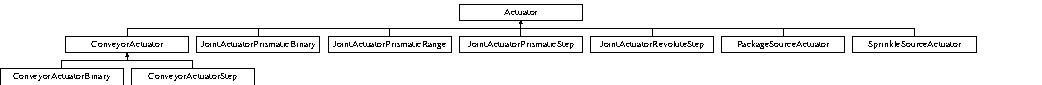
\includegraphics[height=1.147541cm]{classActuator}
\end{center}
\end{figure}
\subsection*{Public Member Functions}
\begin{DoxyCompactItemize}
\item 
\hyperlink{classActuator_a2f4022920c434cd6b3f78a749b60fbfe}{Actuator} (int id)
\item 
virtual \hyperlink{classActuator_ac9dda5313616de651431d103988f6c1b}{$\sim$\-Actuator} ()
\item 
virtual int \hyperlink{classActuator_aa97717414ddb932701fa8c882bc55773}{get\-Id} ()
\item 
virtual string \hyperlink{classActuator_a7d57e5b0684179fe527b7724897a0312}{get\-Name} ()
\item 
virtual void \hyperlink{classActuator_aaa39a438315ac34dbb1a4237bf70ff99}{draw\-Label} ()
\item 
virtual void \hyperlink{classActuator_a6281019cccd4034ab2cf7071defecf70}{set} (signed int value)
\item 
virtual void \hyperlink{classActuator_aabe48a4249a91a4cd1b964001fe754fc}{run} ()
\end{DoxyCompactItemize}
\subsection*{Public Attributes}
\begin{DoxyCompactItemize}
\item 
int \hyperlink{classActuator_aec2f761be4e82de74e986f02e5e77527}{m\-\_\-id}
\item 
b2\-Color \hyperlink{classActuator_ad534cbd18d6df7e5ab080b3628f5522d}{m\-\_\-color}
\item 
b2\-Vec2 \hyperlink{classActuator_ab7e8376ea5e795af2aad96c924253c77}{m\-\_\-position}
\item 
string \hyperlink{classActuator_a1664ca83d9352531527aa66c2f965b7b}{m\-\_\-name}
\end{DoxyCompactItemize}


\subsection{Detailed Description}
Abstract class from which other actuator-\/classes inherit. 

\subsection{Constructor \& Destructor Documentation}
\hypertarget{classActuator_a2f4022920c434cd6b3f78a749b60fbfe}{\index{Actuator@{Actuator}!Actuator@{Actuator}}
\index{Actuator@{Actuator}!Actuator@{Actuator}}
\subsubsection[{Actuator}]{\setlength{\rightskip}{0pt plus 5cm}Actuator\-::\-Actuator (
\begin{DoxyParamCaption}
\item[{int}]{id}
\end{DoxyParamCaption}
)}}\label{classActuator_a2f4022920c434cd6b3f78a749b60fbfe}
\hypertarget{classActuator_ac9dda5313616de651431d103988f6c1b}{\index{Actuator@{Actuator}!$\sim$\-Actuator@{$\sim$\-Actuator}}
\index{$\sim$\-Actuator@{$\sim$\-Actuator}!Actuator@{Actuator}}
\subsubsection[{$\sim$\-Actuator}]{\setlength{\rightskip}{0pt plus 5cm}virtual Actuator\-::$\sim$\-Actuator (
\begin{DoxyParamCaption}
{}
\end{DoxyParamCaption}
)\hspace{0.3cm}{\ttfamily [inline]}, {\ttfamily [virtual]}}}\label{classActuator_ac9dda5313616de651431d103988f6c1b}


\subsection{Member Function Documentation}
\hypertarget{classActuator_aaa39a438315ac34dbb1a4237bf70ff99}{\index{Actuator@{Actuator}!draw\-Label@{draw\-Label}}
\index{draw\-Label@{draw\-Label}!Actuator@{Actuator}}
\subsubsection[{draw\-Label}]{\setlength{\rightskip}{0pt plus 5cm}virtual void Actuator\-::draw\-Label (
\begin{DoxyParamCaption}
{}
\end{DoxyParamCaption}
)\hspace{0.3cm}{\ttfamily [inline]}, {\ttfamily [virtual]}}}\label{classActuator_aaa39a438315ac34dbb1a4237bf70ff99}


Reimplemented in \hyperlink{classSprinkleSourceActuator_ad61ef520615f3ad27964c9388da99825}{Sprinkle\-Source\-Actuator}, \hyperlink{classPackageSourceActuator_ab27c455d40d832ed4558f893f1ed3565}{Package\-Source\-Actuator}, \hyperlink{classJointActuatorRevoluteStep_ab390783e9b495488afa09e8f29aee6d9}{Joint\-Actuator\-Revolute\-Step}, \hyperlink{classJointActuatorPrismaticStep_aecbb187fd46eb1e197a34bcd54aaf4d4}{Joint\-Actuator\-Prismatic\-Step}, \hyperlink{classJointActuatorPrismaticRange_a9daa027177e5bd6c0296b3cf4a76e9ab}{Joint\-Actuator\-Prismatic\-Range}, \hyperlink{classJointActuatorPrismaticBinary_a2c4cd26a0ae47850eca1047ba078a654}{Joint\-Actuator\-Prismatic\-Binary}, and \hyperlink{classConveyorActuator_a92b62d5cb761e808337d3b9de910a543}{Conveyor\-Actuator}.

\hypertarget{classActuator_aa97717414ddb932701fa8c882bc55773}{\index{Actuator@{Actuator}!get\-Id@{get\-Id}}
\index{get\-Id@{get\-Id}!Actuator@{Actuator}}
\subsubsection[{get\-Id}]{\setlength{\rightskip}{0pt plus 5cm}virtual int Actuator\-::get\-Id (
\begin{DoxyParamCaption}
{}
\end{DoxyParamCaption}
)\hspace{0.3cm}{\ttfamily [inline]}, {\ttfamily [virtual]}}}\label{classActuator_aa97717414ddb932701fa8c882bc55773}
\hypertarget{classActuator_a7d57e5b0684179fe527b7724897a0312}{\index{Actuator@{Actuator}!get\-Name@{get\-Name}}
\index{get\-Name@{get\-Name}!Actuator@{Actuator}}
\subsubsection[{get\-Name}]{\setlength{\rightskip}{0pt plus 5cm}virtual string Actuator\-::get\-Name (
\begin{DoxyParamCaption}
{}
\end{DoxyParamCaption}
)\hspace{0.3cm}{\ttfamily [inline]}, {\ttfamily [virtual]}}}\label{classActuator_a7d57e5b0684179fe527b7724897a0312}
\hypertarget{classActuator_aabe48a4249a91a4cd1b964001fe754fc}{\index{Actuator@{Actuator}!run@{run}}
\index{run@{run}!Actuator@{Actuator}}
\subsubsection[{run}]{\setlength{\rightskip}{0pt plus 5cm}virtual void Actuator\-::run (
\begin{DoxyParamCaption}
{}
\end{DoxyParamCaption}
)\hspace{0.3cm}{\ttfamily [inline]}, {\ttfamily [virtual]}}}\label{classActuator_aabe48a4249a91a4cd1b964001fe754fc}


Reimplemented in \hyperlink{classSprinkleSourceActuator_a92ea18d960f132ec493d3b0400a0c504}{Sprinkle\-Source\-Actuator}, \hyperlink{classPackageSourceActuator_a058a225a850f0d49a79f90700ada3254}{Package\-Source\-Actuator}, \hyperlink{classJointActuatorRevoluteStep_a6445fceda983f3fd1f0b280bb03a66af}{Joint\-Actuator\-Revolute\-Step}, \hyperlink{classJointActuatorPrismaticStep_a30a61d48a3719b5d0390be85b7445883}{Joint\-Actuator\-Prismatic\-Step}, \hyperlink{classConveyorActuatorStep_a07d92edbe704485cadea21988d263201}{Conveyor\-Actuator\-Step}, and \hyperlink{classConveyorActuator_a0df274add7b944f869e9486fce8240b1}{Conveyor\-Actuator}.

\hypertarget{classActuator_a6281019cccd4034ab2cf7071defecf70}{\index{Actuator@{Actuator}!set@{set}}
\index{set@{set}!Actuator@{Actuator}}
\subsubsection[{set}]{\setlength{\rightskip}{0pt plus 5cm}virtual void Actuator\-::set (
\begin{DoxyParamCaption}
\item[{signed int}]{value}
\end{DoxyParamCaption}
)\hspace{0.3cm}{\ttfamily [inline]}, {\ttfamily [virtual]}}}\label{classActuator_a6281019cccd4034ab2cf7071defecf70}


Reimplemented in \hyperlink{classSprinkleSourceActuator_a273206caefb1bfa72320f7b096a004ed}{Sprinkle\-Source\-Actuator}, \hyperlink{classPackageSourceActuator_a67e19fb7457c9c29288d8409446756f0}{Package\-Source\-Actuator}, \hyperlink{classJointActuatorRevoluteStep_af72ade5873ae6b2816f1f7c89bf95971}{Joint\-Actuator\-Revolute\-Step}, \hyperlink{classJointActuatorPrismaticStep_ace7839e236e16848375f963697ac408a}{Joint\-Actuator\-Prismatic\-Step}, \hyperlink{classJointActuatorPrismaticRange_a6df9efdb8bf3cea3cffefa977a6f4c02}{Joint\-Actuator\-Prismatic\-Range}, \hyperlink{classJointActuatorPrismaticBinary_a78d1185c3762bb4301f31f0619cded7a}{Joint\-Actuator\-Prismatic\-Binary}, \hyperlink{classConveyorActuatorStep_a7aa64b6b41c86fe4efac32f0090f60f9}{Conveyor\-Actuator\-Step}, \hyperlink{classConveyorActuatorBinary_a7b546c90b95e289cc0b618001fc934f8}{Conveyor\-Actuator\-Binary}, and \hyperlink{classConveyorActuator_a4eeadeec24502aed450880cba04e2784}{Conveyor\-Actuator}.



\subsection{Member Data Documentation}
\hypertarget{classActuator_ad534cbd18d6df7e5ab080b3628f5522d}{\index{Actuator@{Actuator}!m\-\_\-color@{m\-\_\-color}}
\index{m\-\_\-color@{m\-\_\-color}!Actuator@{Actuator}}
\subsubsection[{m\-\_\-color}]{\setlength{\rightskip}{0pt plus 5cm}b2\-Color Actuator\-::m\-\_\-color}}\label{classActuator_ad534cbd18d6df7e5ab080b3628f5522d}
\hypertarget{classActuator_aec2f761be4e82de74e986f02e5e77527}{\index{Actuator@{Actuator}!m\-\_\-id@{m\-\_\-id}}
\index{m\-\_\-id@{m\-\_\-id}!Actuator@{Actuator}}
\subsubsection[{m\-\_\-id}]{\setlength{\rightskip}{0pt plus 5cm}int Actuator\-::m\-\_\-id}}\label{classActuator_aec2f761be4e82de74e986f02e5e77527}
\hypertarget{classActuator_a1664ca83d9352531527aa66c2f965b7b}{\index{Actuator@{Actuator}!m\-\_\-name@{m\-\_\-name}}
\index{m\-\_\-name@{m\-\_\-name}!Actuator@{Actuator}}
\subsubsection[{m\-\_\-name}]{\setlength{\rightskip}{0pt plus 5cm}string Actuator\-::m\-\_\-name}}\label{classActuator_a1664ca83d9352531527aa66c2f965b7b}
\hypertarget{classActuator_ab7e8376ea5e795af2aad96c924253c77}{\index{Actuator@{Actuator}!m\-\_\-position@{m\-\_\-position}}
\index{m\-\_\-position@{m\-\_\-position}!Actuator@{Actuator}}
\subsubsection[{m\-\_\-position}]{\setlength{\rightskip}{0pt plus 5cm}b2\-Vec2 Actuator\-::m\-\_\-position}}\label{classActuator_ab7e8376ea5e795af2aad96c924253c77}


The documentation for this class was generated from the following files\-:\begin{DoxyCompactItemize}
\item 
\hyperlink{Actuators_8h}{Actuators.\-h}\item 
\hyperlink{Actuators_8cpp}{Actuators.\-cpp}\end{DoxyCompactItemize}

\hypertarget{classActuatorSet}{\section{Actuator\-Set Class Reference}
\label{classActuatorSet}\index{Actuator\-Set@{Actuator\-Set}}
}


Draw actuator-\/labels, run actuators and change the state of actuators by id.  




{\ttfamily \#include $<$Actuators.\-h$>$}

\subsection*{Public Member Functions}
\begin{DoxyCompactItemize}
\item 
\hyperlink{classActuatorSet_ab755839440f598cbb8e0ac5a24b74c7d}{Actuator\-Set} ()
\item 
void \hyperlink{classActuatorSet_a5c2f8ee29cc0ab8ea165f24b0592ef65}{add} (\hyperlink{classActuator}{Actuator} $\ast$actuator)
\begin{DoxyCompactList}\small\item\em Add any actuator to the actuator-\/set. \end{DoxyCompactList}\item 
void \hyperlink{classActuatorSet_a55a037ecf2905802d6f89941fd73a61c}{draw\-Labels} ()
\begin{DoxyCompactList}\small\item\em Draw labels of all registered actuators. \end{DoxyCompactList}\item 
void \hyperlink{classActuatorSet_a61e2b64780d67b971cecd0f220e77af6}{write\-Actuator} (signed int id, signed int value)
\begin{DoxyCompactList}\small\item\em Change state of actuator by actuator-\/id. \end{DoxyCompactList}\item 
void \hyperlink{classActuatorSet_ab7f5bb6756d4a5f57dbb94e4f8abcf53}{run} ()
\begin{DoxyCompactList}\small\item\em Run all registered actuators. \end{DoxyCompactList}\end{DoxyCompactItemize}
\subsection*{Public Attributes}
\begin{DoxyCompactItemize}
\item 
vector$<$ \hyperlink{classActuator}{Actuator} $\ast$ $>$ \hyperlink{classActuatorSet_a2696ae7e9eeee0b062e85d68387d6d92}{m\-\_\-actuator}
\end{DoxyCompactItemize}


\subsection{Detailed Description}
Draw actuator-\/labels, run actuators and change the state of actuators by id. 

\subsection{Constructor \& Destructor Documentation}
\hypertarget{classActuatorSet_ab755839440f598cbb8e0ac5a24b74c7d}{\index{Actuator\-Set@{Actuator\-Set}!Actuator\-Set@{Actuator\-Set}}
\index{Actuator\-Set@{Actuator\-Set}!ActuatorSet@{Actuator\-Set}}
\subsubsection[{Actuator\-Set}]{\setlength{\rightskip}{0pt plus 5cm}Actuator\-Set\-::\-Actuator\-Set (
\begin{DoxyParamCaption}
{}
\end{DoxyParamCaption}
)\hspace{0.3cm}{\ttfamily [inline]}}}\label{classActuatorSet_ab755839440f598cbb8e0ac5a24b74c7d}


\subsection{Member Function Documentation}
\hypertarget{classActuatorSet_a5c2f8ee29cc0ab8ea165f24b0592ef65}{\index{Actuator\-Set@{Actuator\-Set}!add@{add}}
\index{add@{add}!ActuatorSet@{Actuator\-Set}}
\subsubsection[{add}]{\setlength{\rightskip}{0pt plus 5cm}void Actuator\-Set\-::add (
\begin{DoxyParamCaption}
\item[{{\bf Actuator} $\ast$}]{actuator}
\end{DoxyParamCaption}
)}}\label{classActuatorSet_a5c2f8ee29cc0ab8ea165f24b0592ef65}


Add any actuator to the actuator-\/set. 

\hypertarget{classActuatorSet_a55a037ecf2905802d6f89941fd73a61c}{\index{Actuator\-Set@{Actuator\-Set}!draw\-Labels@{draw\-Labels}}
\index{draw\-Labels@{draw\-Labels}!ActuatorSet@{Actuator\-Set}}
\subsubsection[{draw\-Labels}]{\setlength{\rightskip}{0pt plus 5cm}void Actuator\-Set\-::draw\-Labels (
\begin{DoxyParamCaption}
{}
\end{DoxyParamCaption}
)}}\label{classActuatorSet_a55a037ecf2905802d6f89941fd73a61c}


Draw labels of all registered actuators. 

\hypertarget{classActuatorSet_ab7f5bb6756d4a5f57dbb94e4f8abcf53}{\index{Actuator\-Set@{Actuator\-Set}!run@{run}}
\index{run@{run}!ActuatorSet@{Actuator\-Set}}
\subsubsection[{run}]{\setlength{\rightskip}{0pt plus 5cm}void Actuator\-Set\-::run (
\begin{DoxyParamCaption}
{}
\end{DoxyParamCaption}
)}}\label{classActuatorSet_ab7f5bb6756d4a5f57dbb94e4f8abcf53}


Run all registered actuators. 

\hypertarget{classActuatorSet_a61e2b64780d67b971cecd0f220e77af6}{\index{Actuator\-Set@{Actuator\-Set}!write\-Actuator@{write\-Actuator}}
\index{write\-Actuator@{write\-Actuator}!ActuatorSet@{Actuator\-Set}}
\subsubsection[{write\-Actuator}]{\setlength{\rightskip}{0pt plus 5cm}void Actuator\-Set\-::write\-Actuator (
\begin{DoxyParamCaption}
\item[{signed int}]{id, }
\item[{signed int}]{value}
\end{DoxyParamCaption}
)}}\label{classActuatorSet_a61e2b64780d67b971cecd0f220e77af6}


Change state of actuator by actuator-\/id. 



\subsection{Member Data Documentation}
\hypertarget{classActuatorSet_a2696ae7e9eeee0b062e85d68387d6d92}{\index{Actuator\-Set@{Actuator\-Set}!m\-\_\-actuator@{m\-\_\-actuator}}
\index{m\-\_\-actuator@{m\-\_\-actuator}!ActuatorSet@{Actuator\-Set}}
\subsubsection[{m\-\_\-actuator}]{\setlength{\rightskip}{0pt plus 5cm}vector$<${\bf Actuator}$\ast$$>$ Actuator\-Set\-::m\-\_\-actuator}}\label{classActuatorSet_a2696ae7e9eeee0b062e85d68387d6d92}


The documentation for this class was generated from the following files\-:\begin{DoxyCompactItemize}
\item 
\hyperlink{Actuators_8h}{Actuators.\-h}\item 
\hyperlink{Actuators_8cpp}{Actuators.\-cpp}\end{DoxyCompactItemize}

\hypertarget{classBeam}{\section{Beam Class Reference}
\label{classBeam}\index{Beam@{Beam}}
}


The beam which the wheels are attached to and which the belt runs along.  




{\ttfamily \#include $<$Conveyor.\-h$>$}

\subsection*{Public Member Functions}
\begin{DoxyCompactItemize}
\item 
\hyperlink{classBeam_a85ec52f2a4eb46b6306b3d3351be4111}{Beam} (b2\-Vec2 p1, b2\-Vec2 p2, float32 width, int cm\-Bits, b2\-World $\ast$world)
\item 
b2\-Vec2 \& \hyperlink{classBeam_a4c0de52fcd115dd4e3267ba99668a45b}{get\-Local\-Anchor1} ()
\item 
b2\-Vec2 \& \hyperlink{classBeam_af96f32192c1729ba2ba6f8762f6d714a}{get\-Local\-Anchor2} ()
\item 
b2\-Body $\ast$ \hyperlink{classBeam_acdfad0d43f2aaf67e4238129c7e4215d}{get\-Body} ()
\end{DoxyCompactItemize}
\subsection*{Private Attributes}
\begin{DoxyCompactItemize}
\item 
b2\-Body $\ast$ \hyperlink{classBeam_a282db593ede22f681dbf57729fd203b0}{m\-\_\-body}
\item 
b2\-Vec2 \hyperlink{classBeam_a4155af3bd2f382a56d5cbf275b626a22}{m\-\_\-local\-Anchor1}
\item 
b2\-Vec2 \hyperlink{classBeam_a00a74039f9b2feb4e440200cca2046b2}{m\-\_\-local\-Anchor2}
\end{DoxyCompactItemize}


\subsection{Detailed Description}
The beam which the wheels are attached to and which the belt runs along. 

\subsection{Constructor \& Destructor Documentation}
\hypertarget{classBeam_a85ec52f2a4eb46b6306b3d3351be4111}{\index{Beam@{Beam}!Beam@{Beam}}
\index{Beam@{Beam}!Beam@{Beam}}
\subsubsection[{Beam}]{\setlength{\rightskip}{0pt plus 5cm}Beam\-::\-Beam (
\begin{DoxyParamCaption}
\item[{b2\-Vec2}]{p1, }
\item[{b2\-Vec2}]{p2, }
\item[{float32}]{width, }
\item[{int}]{cm\-Bits, }
\item[{b2\-World $\ast$}]{world}
\end{DoxyParamCaption}
)}}\label{classBeam_a85ec52f2a4eb46b6306b3d3351be4111}


\subsection{Member Function Documentation}
\hypertarget{classBeam_acdfad0d43f2aaf67e4238129c7e4215d}{\index{Beam@{Beam}!get\-Body@{get\-Body}}
\index{get\-Body@{get\-Body}!Beam@{Beam}}
\subsubsection[{get\-Body}]{\setlength{\rightskip}{0pt plus 5cm}b2\-Body$\ast$ Beam\-::get\-Body (
\begin{DoxyParamCaption}
{}
\end{DoxyParamCaption}
)\hspace{0.3cm}{\ttfamily [inline]}}}\label{classBeam_acdfad0d43f2aaf67e4238129c7e4215d}
\hypertarget{classBeam_a4c0de52fcd115dd4e3267ba99668a45b}{\index{Beam@{Beam}!get\-Local\-Anchor1@{get\-Local\-Anchor1}}
\index{get\-Local\-Anchor1@{get\-Local\-Anchor1}!Beam@{Beam}}
\subsubsection[{get\-Local\-Anchor1}]{\setlength{\rightskip}{0pt plus 5cm}b2\-Vec2\& Beam\-::get\-Local\-Anchor1 (
\begin{DoxyParamCaption}
{}
\end{DoxyParamCaption}
)\hspace{0.3cm}{\ttfamily [inline]}}}\label{classBeam_a4c0de52fcd115dd4e3267ba99668a45b}
\hypertarget{classBeam_af96f32192c1729ba2ba6f8762f6d714a}{\index{Beam@{Beam}!get\-Local\-Anchor2@{get\-Local\-Anchor2}}
\index{get\-Local\-Anchor2@{get\-Local\-Anchor2}!Beam@{Beam}}
\subsubsection[{get\-Local\-Anchor2}]{\setlength{\rightskip}{0pt plus 5cm}b2\-Vec2\& Beam\-::get\-Local\-Anchor2 (
\begin{DoxyParamCaption}
{}
\end{DoxyParamCaption}
)\hspace{0.3cm}{\ttfamily [inline]}}}\label{classBeam_af96f32192c1729ba2ba6f8762f6d714a}


\subsection{Member Data Documentation}
\hypertarget{classBeam_a282db593ede22f681dbf57729fd203b0}{\index{Beam@{Beam}!m\-\_\-body@{m\-\_\-body}}
\index{m\-\_\-body@{m\-\_\-body}!Beam@{Beam}}
\subsubsection[{m\-\_\-body}]{\setlength{\rightskip}{0pt plus 5cm}b2\-Body$\ast$ Beam\-::m\-\_\-body\hspace{0.3cm}{\ttfamily [private]}}}\label{classBeam_a282db593ede22f681dbf57729fd203b0}
\hypertarget{classBeam_a4155af3bd2f382a56d5cbf275b626a22}{\index{Beam@{Beam}!m\-\_\-local\-Anchor1@{m\-\_\-local\-Anchor1}}
\index{m\-\_\-local\-Anchor1@{m\-\_\-local\-Anchor1}!Beam@{Beam}}
\subsubsection[{m\-\_\-local\-Anchor1}]{\setlength{\rightskip}{0pt plus 5cm}b2\-Vec2 Beam\-::m\-\_\-local\-Anchor1\hspace{0.3cm}{\ttfamily [private]}}}\label{classBeam_a4155af3bd2f382a56d5cbf275b626a22}
\hypertarget{classBeam_a00a74039f9b2feb4e440200cca2046b2}{\index{Beam@{Beam}!m\-\_\-local\-Anchor2@{m\-\_\-local\-Anchor2}}
\index{m\-\_\-local\-Anchor2@{m\-\_\-local\-Anchor2}!Beam@{Beam}}
\subsubsection[{m\-\_\-local\-Anchor2}]{\setlength{\rightskip}{0pt plus 5cm}b2\-Vec2 Beam\-::m\-\_\-local\-Anchor2\hspace{0.3cm}{\ttfamily [private]}}}\label{classBeam_a00a74039f9b2feb4e440200cca2046b2}


The documentation for this class was generated from the following files\-:\begin{DoxyCompactItemize}
\item 
\hyperlink{Conveyor_8h}{Conveyor.\-h}\item 
\hyperlink{Conveyor_8cpp}{Conveyor.\-cpp}\end{DoxyCompactItemize}

\hypertarget{classCommandSequenceInterpreter}{\section{Command\-Sequence\-Interpreter Class Reference}
\label{classCommandSequenceInterpreter}\index{Command\-Sequence\-Interpreter@{Command\-Sequence\-Interpreter}}
}


Use keyboard-\/ or terminal-\/input to control the actuator-\/ and sensor-\/sets.  




{\ttfamily \#include $<$Command\-Sequence\-Interpreter.\-h$>$}

\subsection*{Public Types}
\begin{DoxyCompactItemize}
\item 
enum \hyperlink{classCommandSequenceInterpreter_a651640c84d800a896ccd8291a93128a0}{t\-\_\-read\-State} \{ \hyperlink{classCommandSequenceInterpreter_a651640c84d800a896ccd8291a93128a0a658adac09e435337a98ccbe2f74cdafa}{st\-\_\-wait\-\_\-for\-\_\-new\-\_\-command}, 
\hyperlink{classCommandSequenceInterpreter_a651640c84d800a896ccd8291a93128a0a5b0174436df6e847d871f05feddc755a}{st\-\_\-read\-\_\-parameter}
 \}
\item 
enum \hyperlink{classCommandSequenceInterpreter_a96f5e5d9fa213d5e6a9bb0e3fb7fabd8}{t\-\_\-command\-Type} \{ \hyperlink{classCommandSequenceInterpreter_a96f5e5d9fa213d5e6a9bb0e3fb7fabd8ab9a8f3bd83268621ea2e2ec5ac19e900}{e\-\_\-write\-Actuator}, 
\hyperlink{classCommandSequenceInterpreter_a96f5e5d9fa213d5e6a9bb0e3fb7fabd8a6bc4cdc026336f37ebec76e878ca3718}{e\-\_\-read\-Sensor}
 \}
\end{DoxyCompactItemize}
\subsection*{Public Member Functions}
\begin{DoxyCompactItemize}
\item 
\hyperlink{classCommandSequenceInterpreter_ae14fc280499fea9ae536b6bdfb40f0f9}{Command\-Sequence\-Interpreter} (\hyperlink{classActuatorSet}{Actuator\-Set} $\ast$actuator\-Set, \hyperlink{classSensorSet}{Sensor\-Set} $\ast$sensor\-Set)
\item 
void \hyperlink{classCommandSequenceInterpreter_a50bffc4e9f2b6953ed64cc62f6c65b9d}{interpret} (unsigned char key)
\end{DoxyCompactItemize}
\subsection*{Public Attributes}
\begin{DoxyCompactItemize}
\item 
\hyperlink{classCommandSequenceInterpreter_a96f5e5d9fa213d5e6a9bb0e3fb7fabd8}{t\-\_\-command\-Type} \hyperlink{classCommandSequenceInterpreter_a67f17cd12035c3177dec4ad7199dff09}{m\-\_\-command\-Type}
\item 
\hyperlink{classCommandSequenceInterpreter_a651640c84d800a896ccd8291a93128a0}{t\-\_\-read\-State} \hyperlink{classCommandSequenceInterpreter_ac230cd37bfd33ff720a04142ba9b13fc}{m\-\_\-read\-State}
\item 
stringstream \hyperlink{classCommandSequenceInterpreter_af00adda23c01ffa7092ac6c8304de4fd}{m\-\_\-ss}
\item 
vector$<$ string $>$ \hyperlink{classCommandSequenceInterpreter_acd419ae2ac997f8b8c59003b5e2c4a32}{m\-\_\-parameter}
\item 
\hyperlink{classActuatorSet}{Actuator\-Set} $\ast$ \hyperlink{classCommandSequenceInterpreter_aab92295e940532f6175327d6a03e7d67}{m\-\_\-actuator\-Set}
\item 
\hyperlink{classSensorSet}{Sensor\-Set} $\ast$ \hyperlink{classCommandSequenceInterpreter_ad0c5aa0524c53759ec691efebcca5233}{m\-\_\-sensor\-Set}
\end{DoxyCompactItemize}


\subsection{Detailed Description}
Use keyboard-\/ or terminal-\/input to control the actuator-\/ and sensor-\/sets. 

\subsection{Member Enumeration Documentation}
\hypertarget{classCommandSequenceInterpreter_a96f5e5d9fa213d5e6a9bb0e3fb7fabd8}{\index{Command\-Sequence\-Interpreter@{Command\-Sequence\-Interpreter}!t\-\_\-command\-Type@{t\-\_\-command\-Type}}
\index{t\-\_\-command\-Type@{t\-\_\-command\-Type}!CommandSequenceInterpreter@{Command\-Sequence\-Interpreter}}
\subsubsection[{t\-\_\-command\-Type}]{\setlength{\rightskip}{0pt plus 5cm}enum {\bf Command\-Sequence\-Interpreter\-::t\-\_\-command\-Type}}}\label{classCommandSequenceInterpreter_a96f5e5d9fa213d5e6a9bb0e3fb7fabd8}
\begin{Desc}
\item[Enumerator\-: ]\par
\begin{description}
\index{e\-\_\-write\-Actuator@{e\-\_\-write\-Actuator}!Command\-Sequence\-Interpreter@{Command\-Sequence\-Interpreter}}\index{Command\-Sequence\-Interpreter@{Command\-Sequence\-Interpreter}!e\-\_\-write\-Actuator@{e\-\_\-write\-Actuator}}\item[{\em 
\hypertarget{classCommandSequenceInterpreter_a96f5e5d9fa213d5e6a9bb0e3fb7fabd8ab9a8f3bd83268621ea2e2ec5ac19e900}{e\-\_\-write\-Actuator}\label{classCommandSequenceInterpreter_a96f5e5d9fa213d5e6a9bb0e3fb7fabd8ab9a8f3bd83268621ea2e2ec5ac19e900}
}]\index{e\-\_\-read\-Sensor@{e\-\_\-read\-Sensor}!Command\-Sequence\-Interpreter@{Command\-Sequence\-Interpreter}}\index{Command\-Sequence\-Interpreter@{Command\-Sequence\-Interpreter}!e\-\_\-read\-Sensor@{e\-\_\-read\-Sensor}}\item[{\em 
\hypertarget{classCommandSequenceInterpreter_a96f5e5d9fa213d5e6a9bb0e3fb7fabd8a6bc4cdc026336f37ebec76e878ca3718}{e\-\_\-read\-Sensor}\label{classCommandSequenceInterpreter_a96f5e5d9fa213d5e6a9bb0e3fb7fabd8a6bc4cdc026336f37ebec76e878ca3718}
}]\end{description}
\end{Desc}

\hypertarget{classCommandSequenceInterpreter_a651640c84d800a896ccd8291a93128a0}{\index{Command\-Sequence\-Interpreter@{Command\-Sequence\-Interpreter}!t\-\_\-read\-State@{t\-\_\-read\-State}}
\index{t\-\_\-read\-State@{t\-\_\-read\-State}!CommandSequenceInterpreter@{Command\-Sequence\-Interpreter}}
\subsubsection[{t\-\_\-read\-State}]{\setlength{\rightskip}{0pt plus 5cm}enum {\bf Command\-Sequence\-Interpreter\-::t\-\_\-read\-State}}}\label{classCommandSequenceInterpreter_a651640c84d800a896ccd8291a93128a0}
\begin{Desc}
\item[Enumerator\-: ]\par
\begin{description}
\index{st\-\_\-wait\-\_\-for\-\_\-new\-\_\-command@{st\-\_\-wait\-\_\-for\-\_\-new\-\_\-command}!Command\-Sequence\-Interpreter@{Command\-Sequence\-Interpreter}}\index{Command\-Sequence\-Interpreter@{Command\-Sequence\-Interpreter}!st\-\_\-wait\-\_\-for\-\_\-new\-\_\-command@{st\-\_\-wait\-\_\-for\-\_\-new\-\_\-command}}\item[{\em 
\hypertarget{classCommandSequenceInterpreter_a651640c84d800a896ccd8291a93128a0a658adac09e435337a98ccbe2f74cdafa}{st\-\_\-wait\-\_\-for\-\_\-new\-\_\-command}\label{classCommandSequenceInterpreter_a651640c84d800a896ccd8291a93128a0a658adac09e435337a98ccbe2f74cdafa}
}]\index{st\-\_\-read\-\_\-parameter@{st\-\_\-read\-\_\-parameter}!Command\-Sequence\-Interpreter@{Command\-Sequence\-Interpreter}}\index{Command\-Sequence\-Interpreter@{Command\-Sequence\-Interpreter}!st\-\_\-read\-\_\-parameter@{st\-\_\-read\-\_\-parameter}}\item[{\em 
\hypertarget{classCommandSequenceInterpreter_a651640c84d800a896ccd8291a93128a0a5b0174436df6e847d871f05feddc755a}{st\-\_\-read\-\_\-parameter}\label{classCommandSequenceInterpreter_a651640c84d800a896ccd8291a93128a0a5b0174436df6e847d871f05feddc755a}
}]\end{description}
\end{Desc}



\subsection{Constructor \& Destructor Documentation}
\hypertarget{classCommandSequenceInterpreter_ae14fc280499fea9ae536b6bdfb40f0f9}{\index{Command\-Sequence\-Interpreter@{Command\-Sequence\-Interpreter}!Command\-Sequence\-Interpreter@{Command\-Sequence\-Interpreter}}
\index{Command\-Sequence\-Interpreter@{Command\-Sequence\-Interpreter}!CommandSequenceInterpreter@{Command\-Sequence\-Interpreter}}
\subsubsection[{Command\-Sequence\-Interpreter}]{\setlength{\rightskip}{0pt plus 5cm}Command\-Sequence\-Interpreter\-::\-Command\-Sequence\-Interpreter (
\begin{DoxyParamCaption}
\item[{{\bf Actuator\-Set} $\ast$}]{actuator\-Set, }
\item[{{\bf Sensor\-Set} $\ast$}]{sensor\-Set}
\end{DoxyParamCaption}
)}}\label{classCommandSequenceInterpreter_ae14fc280499fea9ae536b6bdfb40f0f9}


\subsection{Member Function Documentation}
\hypertarget{classCommandSequenceInterpreter_a50bffc4e9f2b6953ed64cc62f6c65b9d}{\index{Command\-Sequence\-Interpreter@{Command\-Sequence\-Interpreter}!interpret@{interpret}}
\index{interpret@{interpret}!CommandSequenceInterpreter@{Command\-Sequence\-Interpreter}}
\subsubsection[{interpret}]{\setlength{\rightskip}{0pt plus 5cm}void Command\-Sequence\-Interpreter\-::interpret (
\begin{DoxyParamCaption}
\item[{unsigned char}]{key}
\end{DoxyParamCaption}
)}}\label{classCommandSequenceInterpreter_a50bffc4e9f2b6953ed64cc62f6c65b9d}


\subsection{Member Data Documentation}
\hypertarget{classCommandSequenceInterpreter_aab92295e940532f6175327d6a03e7d67}{\index{Command\-Sequence\-Interpreter@{Command\-Sequence\-Interpreter}!m\-\_\-actuator\-Set@{m\-\_\-actuator\-Set}}
\index{m\-\_\-actuator\-Set@{m\-\_\-actuator\-Set}!CommandSequenceInterpreter@{Command\-Sequence\-Interpreter}}
\subsubsection[{m\-\_\-actuator\-Set}]{\setlength{\rightskip}{0pt plus 5cm}{\bf Actuator\-Set}$\ast$ Command\-Sequence\-Interpreter\-::m\-\_\-actuator\-Set}}\label{classCommandSequenceInterpreter_aab92295e940532f6175327d6a03e7d67}
\hypertarget{classCommandSequenceInterpreter_a67f17cd12035c3177dec4ad7199dff09}{\index{Command\-Sequence\-Interpreter@{Command\-Sequence\-Interpreter}!m\-\_\-command\-Type@{m\-\_\-command\-Type}}
\index{m\-\_\-command\-Type@{m\-\_\-command\-Type}!CommandSequenceInterpreter@{Command\-Sequence\-Interpreter}}
\subsubsection[{m\-\_\-command\-Type}]{\setlength{\rightskip}{0pt plus 5cm}{\bf t\-\_\-command\-Type} Command\-Sequence\-Interpreter\-::m\-\_\-command\-Type}}\label{classCommandSequenceInterpreter_a67f17cd12035c3177dec4ad7199dff09}
\hypertarget{classCommandSequenceInterpreter_acd419ae2ac997f8b8c59003b5e2c4a32}{\index{Command\-Sequence\-Interpreter@{Command\-Sequence\-Interpreter}!m\-\_\-parameter@{m\-\_\-parameter}}
\index{m\-\_\-parameter@{m\-\_\-parameter}!CommandSequenceInterpreter@{Command\-Sequence\-Interpreter}}
\subsubsection[{m\-\_\-parameter}]{\setlength{\rightskip}{0pt plus 5cm}vector$<$string$>$ Command\-Sequence\-Interpreter\-::m\-\_\-parameter}}\label{classCommandSequenceInterpreter_acd419ae2ac997f8b8c59003b5e2c4a32}
\hypertarget{classCommandSequenceInterpreter_ac230cd37bfd33ff720a04142ba9b13fc}{\index{Command\-Sequence\-Interpreter@{Command\-Sequence\-Interpreter}!m\-\_\-read\-State@{m\-\_\-read\-State}}
\index{m\-\_\-read\-State@{m\-\_\-read\-State}!CommandSequenceInterpreter@{Command\-Sequence\-Interpreter}}
\subsubsection[{m\-\_\-read\-State}]{\setlength{\rightskip}{0pt plus 5cm}{\bf t\-\_\-read\-State} Command\-Sequence\-Interpreter\-::m\-\_\-read\-State}}\label{classCommandSequenceInterpreter_ac230cd37bfd33ff720a04142ba9b13fc}
\hypertarget{classCommandSequenceInterpreter_ad0c5aa0524c53759ec691efebcca5233}{\index{Command\-Sequence\-Interpreter@{Command\-Sequence\-Interpreter}!m\-\_\-sensor\-Set@{m\-\_\-sensor\-Set}}
\index{m\-\_\-sensor\-Set@{m\-\_\-sensor\-Set}!CommandSequenceInterpreter@{Command\-Sequence\-Interpreter}}
\subsubsection[{m\-\_\-sensor\-Set}]{\setlength{\rightskip}{0pt plus 5cm}{\bf Sensor\-Set}$\ast$ Command\-Sequence\-Interpreter\-::m\-\_\-sensor\-Set}}\label{classCommandSequenceInterpreter_ad0c5aa0524c53759ec691efebcca5233}
\hypertarget{classCommandSequenceInterpreter_af00adda23c01ffa7092ac6c8304de4fd}{\index{Command\-Sequence\-Interpreter@{Command\-Sequence\-Interpreter}!m\-\_\-ss@{m\-\_\-ss}}
\index{m\-\_\-ss@{m\-\_\-ss}!CommandSequenceInterpreter@{Command\-Sequence\-Interpreter}}
\subsubsection[{m\-\_\-ss}]{\setlength{\rightskip}{0pt plus 5cm}stringstream Command\-Sequence\-Interpreter\-::m\-\_\-ss}}\label{classCommandSequenceInterpreter_af00adda23c01ffa7092ac6c8304de4fd}


The documentation for this class was generated from the following files\-:\begin{DoxyCompactItemize}
\item 
\hyperlink{CommandSequenceInterpreter_8h}{Command\-Sequence\-Interpreter.\-h}\item 
\hyperlink{CommandSequenceInterpreter_8cpp}{Command\-Sequence\-Interpreter.\-cpp}\end{DoxyCompactItemize}

\hypertarget{classCommunicator}{\section{Communicator Class Reference}
\label{classCommunicator}\index{Communicator@{Communicator}}
}


Read frowm and write to an arbitrary serial-\/port.  




{\ttfamily \#include $<$Communicator.\-h$>$}

\subsection*{Public Member Functions}
\begin{DoxyCompactItemize}
\item 
\hyperlink{classCommunicator_a9376e2a4cfde05f3bcbae03523f47f09}{Communicator} (string serieport)
\begin{DoxyCompactList}\small\item\em Create a \hyperlink{classCommunicator}{Communicator} instance and place it at a specific serialport. \end{DoxyCompactList}\item 
void \hyperlink{classCommunicator_a99aabd49f9b816a256035130ed59d1c1}{init} (string serieport)
\begin{DoxyCompactList}\small\item\em Initialize the serialport. \end{DoxyCompactList}\item 
void \hyperlink{classCommunicator_a5a4b8c0d0d2a56c1e66b6baaa5dd0d9a}{write} (const unsigned char c)
\begin{DoxyCompactList}\small\item\em Write a character to the serialport. \end{DoxyCompactList}\item 
void \hyperlink{classCommunicator_aae6febfbbaadf6b7a53dd6718dc1fc26}{write} (string str)
\begin{DoxyCompactList}\small\item\em Write a string to the serialport. \end{DoxyCompactList}\item 
void \hyperlink{classCommunicator_a453c83fb4fcf3b6acf6e26269bbcb743}{print} (char $\ast$format,...)
\item 
bool \hyperlink{classCommunicator_ab8208da85e32d5802b6dcae11e5ddf3d}{data\-Is\-Present} ()
\begin{DoxyCompactList}\small\item\em Check if incoming data exist. \end{DoxyCompactList}\item 
unsigned char \hyperlink{classCommunicator_a8592dcf1ef7cd278a3619a5735ff2b2b}{read} ()
\begin{DoxyCompactList}\small\item\em Read a char from incoming fifo-\/buffer. \end{DoxyCompactList}\item 
void \hyperlink{classCommunicator_a0e202fdfbc9ad191260b4da285d2f071}{close} ()
\begin{DoxyCompactList}\small\item\em Close serialport. \end{DoxyCompactList}\item 
bool \hyperlink{classCommunicator_a7aaa04bd32a78e8b5aa0d79b80b87e52}{active} ()
\begin{DoxyCompactList}\small\item\em Check if port in use. \end{DoxyCompactList}\end{DoxyCompactItemize}
\subsection*{Private Member Functions}
\begin{DoxyCompactItemize}
\item 
void \hyperlink{classCommunicator_af2d0f85b4fd75f457283448bec474d0e}{read\-\_\-start} (void)
\item 
void \hyperlink{classCommunicator_aacbd7b17b825522c324170422989b0dd}{read\-\_\-complete} (const boost\-::system\-::error\-\_\-code \&error, size\-\_\-t bytes\-\_\-transferred)
\item 
void \hyperlink{classCommunicator_af7dd39cc1a386cb9fb1a68715be7ae7a}{do\-\_\-write} (const unsigned char c)
\item 
void \hyperlink{classCommunicator_a949b951edc82d1b5174071b5204156eb}{write\-\_\-start} (void)
\item 
void \hyperlink{classCommunicator_a179b10517097859b289b9108ea2433b7}{write\-\_\-complete} (const boost\-::system\-::error\-\_\-code \&error)
\item 
void \hyperlink{classCommunicator_a39081affb66ee804daed1850faee4cdc}{do\-\_\-close} (const boost\-::system\-::error\-\_\-code \&error)
\end{DoxyCompactItemize}
\subsection*{Private Attributes}
\begin{DoxyCompactItemize}
\item 
io\-\_\-service \hyperlink{classCommunicator_acae03d9f34724b3fcaf98f92c0640e51}{m\-\_\-io}
\item 
serial\-\_\-port \hyperlink{classCommunicator_ad78da07df6c7551bdc4caefd508f97d1}{m\-\_\-port}
\item 
bool \hyperlink{classCommunicator_acbac815df12652c546240cc172ddaf33}{m\-\_\-data\-Is\-Present}
\item 
thread \hyperlink{classCommunicator_a5418b61d132b1e5ff573d7eb7a7e2e0c}{communication\-Thread}
\item 
deque$<$ unsigned char $>$ \hyperlink{classCommunicator_a8f027326373947bb29c68c64e27d7b6a}{m\-\_\-fifo\-Write}
\item 
deque$<$ unsigned char $>$ \hyperlink{classCommunicator_af3f7e36ef85b0ca55d9720b24c94a3d5}{m\-\_\-fifo\-Read}
\item 
unsigned char \hyperlink{classCommunicator_a6d28d139d03917fa04f9b3c9460dcaae}{read\-\_\-msg\-\_\-} \mbox{[}\hyperlink{classCommunicator_a1fa795c1542a7fff4a6b2b66e137b55d}{max\-\_\-read\-\_\-length}\mbox{]}
\item 
bool \hyperlink{classCommunicator_a42a770b0ce7f2b683e4bc1d0f887f14c}{m\-\_\-active}
\end{DoxyCompactItemize}
\subsection*{Static Private Attributes}
\begin{DoxyCompactItemize}
\item 
static const int \hyperlink{classCommunicator_a1fa795c1542a7fff4a6b2b66e137b55d}{max\-\_\-read\-\_\-length} = 512
\end{DoxyCompactItemize}


\subsection{Detailed Description}
Read frowm and write to an arbitrary serial-\/port. 

\subsection{Constructor \& Destructor Documentation}
\hypertarget{classCommunicator_a9376e2a4cfde05f3bcbae03523f47f09}{\index{Communicator@{Communicator}!Communicator@{Communicator}}
\index{Communicator@{Communicator}!Communicator@{Communicator}}
\subsubsection[{Communicator}]{\setlength{\rightskip}{0pt plus 5cm}Communicator\-::\-Communicator (
\begin{DoxyParamCaption}
\item[{string}]{serieport}
\end{DoxyParamCaption}
)}}\label{classCommunicator_a9376e2a4cfde05f3bcbae03523f47f09}


Create a \hyperlink{classCommunicator}{Communicator} instance and place it at a specific serialport. 


\begin{DoxyParams}{Parameters}
{\em serieport} & The serialport in form of a string. E.\-g C\-O\-M1 on windows or /dev/tty\-S0 on linux. \\
\hline
\end{DoxyParams}


\subsection{Member Function Documentation}
\hypertarget{classCommunicator_a7aaa04bd32a78e8b5aa0d79b80b87e52}{\index{Communicator@{Communicator}!active@{active}}
\index{active@{active}!Communicator@{Communicator}}
\subsubsection[{active}]{\setlength{\rightskip}{0pt plus 5cm}bool Communicator\-::active (
\begin{DoxyParamCaption}
{}
\end{DoxyParamCaption}
)\hspace{0.3cm}{\ttfamily [inline]}}}\label{classCommunicator_a7aaa04bd32a78e8b5aa0d79b80b87e52}


Check if port in use. 

\hypertarget{classCommunicator_a0e202fdfbc9ad191260b4da285d2f071}{\index{Communicator@{Communicator}!close@{close}}
\index{close@{close}!Communicator@{Communicator}}
\subsubsection[{close}]{\setlength{\rightskip}{0pt plus 5cm}void Communicator\-::close (
\begin{DoxyParamCaption}
{}
\end{DoxyParamCaption}
)}}\label{classCommunicator_a0e202fdfbc9ad191260b4da285d2f071}


Close serialport. 

\hypertarget{classCommunicator_ab8208da85e32d5802b6dcae11e5ddf3d}{\index{Communicator@{Communicator}!data\-Is\-Present@{data\-Is\-Present}}
\index{data\-Is\-Present@{data\-Is\-Present}!Communicator@{Communicator}}
\subsubsection[{data\-Is\-Present}]{\setlength{\rightskip}{0pt plus 5cm}bool Communicator\-::data\-Is\-Present (
\begin{DoxyParamCaption}
{}
\end{DoxyParamCaption}
)}}\label{classCommunicator_ab8208da85e32d5802b6dcae11e5ddf3d}


Check if incoming data exist. 

\hypertarget{classCommunicator_a39081affb66ee804daed1850faee4cdc}{\index{Communicator@{Communicator}!do\-\_\-close@{do\-\_\-close}}
\index{do\-\_\-close@{do\-\_\-close}!Communicator@{Communicator}}
\subsubsection[{do\-\_\-close}]{\setlength{\rightskip}{0pt plus 5cm}void Communicator\-::do\-\_\-close (
\begin{DoxyParamCaption}
\item[{const boost\-::system\-::error\-\_\-code \&}]{error}
\end{DoxyParamCaption}
)\hspace{0.3cm}{\ttfamily [private]}}}\label{classCommunicator_a39081affb66ee804daed1850faee4cdc}
\hypertarget{classCommunicator_af7dd39cc1a386cb9fb1a68715be7ae7a}{\index{Communicator@{Communicator}!do\-\_\-write@{do\-\_\-write}}
\index{do\-\_\-write@{do\-\_\-write}!Communicator@{Communicator}}
\subsubsection[{do\-\_\-write}]{\setlength{\rightskip}{0pt plus 5cm}void Communicator\-::do\-\_\-write (
\begin{DoxyParamCaption}
\item[{const unsigned char}]{c}
\end{DoxyParamCaption}
)\hspace{0.3cm}{\ttfamily [private]}}}\label{classCommunicator_af7dd39cc1a386cb9fb1a68715be7ae7a}
\hypertarget{classCommunicator_a99aabd49f9b816a256035130ed59d1c1}{\index{Communicator@{Communicator}!init@{init}}
\index{init@{init}!Communicator@{Communicator}}
\subsubsection[{init}]{\setlength{\rightskip}{0pt plus 5cm}void Communicator\-::init (
\begin{DoxyParamCaption}
\item[{string}]{serieport}
\end{DoxyParamCaption}
)}}\label{classCommunicator_a99aabd49f9b816a256035130ed59d1c1}


Initialize the serialport. 

\hypertarget{classCommunicator_a453c83fb4fcf3b6acf6e26269bbcb743}{\index{Communicator@{Communicator}!print@{print}}
\index{print@{print}!Communicator@{Communicator}}
\subsubsection[{print}]{\setlength{\rightskip}{0pt plus 5cm}void Communicator\-::print (
\begin{DoxyParamCaption}
\item[{char $\ast$}]{format, }
\item[{}]{...}
\end{DoxyParamCaption}
)}}\label{classCommunicator_a453c83fb4fcf3b6acf6e26269bbcb743}
Write a formated string to the serialport \hypertarget{classCommunicator_a8592dcf1ef7cd278a3619a5735ff2b2b}{\index{Communicator@{Communicator}!read@{read}}
\index{read@{read}!Communicator@{Communicator}}
\subsubsection[{read}]{\setlength{\rightskip}{0pt plus 5cm}unsigned char Communicator\-::read (
\begin{DoxyParamCaption}
{}
\end{DoxyParamCaption}
)}}\label{classCommunicator_a8592dcf1ef7cd278a3619a5735ff2b2b}


Read a char from incoming fifo-\/buffer. 

\hypertarget{classCommunicator_aacbd7b17b825522c324170422989b0dd}{\index{Communicator@{Communicator}!read\-\_\-complete@{read\-\_\-complete}}
\index{read\-\_\-complete@{read\-\_\-complete}!Communicator@{Communicator}}
\subsubsection[{read\-\_\-complete}]{\setlength{\rightskip}{0pt plus 5cm}void Communicator\-::read\-\_\-complete (
\begin{DoxyParamCaption}
\item[{const boost\-::system\-::error\-\_\-code \&}]{error, }
\item[{size\-\_\-t}]{bytes\-\_\-transferred}
\end{DoxyParamCaption}
)\hspace{0.3cm}{\ttfamily [private]}}}\label{classCommunicator_aacbd7b17b825522c324170422989b0dd}
\hypertarget{classCommunicator_af2d0f85b4fd75f457283448bec474d0e}{\index{Communicator@{Communicator}!read\-\_\-start@{read\-\_\-start}}
\index{read\-\_\-start@{read\-\_\-start}!Communicator@{Communicator}}
\subsubsection[{read\-\_\-start}]{\setlength{\rightskip}{0pt plus 5cm}void Communicator\-::read\-\_\-start (
\begin{DoxyParamCaption}
\item[{void}]{}
\end{DoxyParamCaption}
)\hspace{0.3cm}{\ttfamily [private]}}}\label{classCommunicator_af2d0f85b4fd75f457283448bec474d0e}
\hypertarget{classCommunicator_a5a4b8c0d0d2a56c1e66b6baaa5dd0d9a}{\index{Communicator@{Communicator}!write@{write}}
\index{write@{write}!Communicator@{Communicator}}
\subsubsection[{write}]{\setlength{\rightskip}{0pt plus 5cm}void Communicator\-::write (
\begin{DoxyParamCaption}
\item[{const unsigned char}]{c}
\end{DoxyParamCaption}
)}}\label{classCommunicator_a5a4b8c0d0d2a56c1e66b6baaa5dd0d9a}


Write a character to the serialport. 

\hypertarget{classCommunicator_aae6febfbbaadf6b7a53dd6718dc1fc26}{\index{Communicator@{Communicator}!write@{write}}
\index{write@{write}!Communicator@{Communicator}}
\subsubsection[{write}]{\setlength{\rightskip}{0pt plus 5cm}void Communicator\-::write (
\begin{DoxyParamCaption}
\item[{string}]{str}
\end{DoxyParamCaption}
)}}\label{classCommunicator_aae6febfbbaadf6b7a53dd6718dc1fc26}


Write a string to the serialport. 

\hypertarget{classCommunicator_a179b10517097859b289b9108ea2433b7}{\index{Communicator@{Communicator}!write\-\_\-complete@{write\-\_\-complete}}
\index{write\-\_\-complete@{write\-\_\-complete}!Communicator@{Communicator}}
\subsubsection[{write\-\_\-complete}]{\setlength{\rightskip}{0pt plus 5cm}void Communicator\-::write\-\_\-complete (
\begin{DoxyParamCaption}
\item[{const boost\-::system\-::error\-\_\-code \&}]{error}
\end{DoxyParamCaption}
)\hspace{0.3cm}{\ttfamily [private]}}}\label{classCommunicator_a179b10517097859b289b9108ea2433b7}
\hypertarget{classCommunicator_a949b951edc82d1b5174071b5204156eb}{\index{Communicator@{Communicator}!write\-\_\-start@{write\-\_\-start}}
\index{write\-\_\-start@{write\-\_\-start}!Communicator@{Communicator}}
\subsubsection[{write\-\_\-start}]{\setlength{\rightskip}{0pt plus 5cm}void Communicator\-::write\-\_\-start (
\begin{DoxyParamCaption}
\item[{void}]{}
\end{DoxyParamCaption}
)\hspace{0.3cm}{\ttfamily [private]}}}\label{classCommunicator_a949b951edc82d1b5174071b5204156eb}


\subsection{Member Data Documentation}
\hypertarget{classCommunicator_a5418b61d132b1e5ff573d7eb7a7e2e0c}{\index{Communicator@{Communicator}!communication\-Thread@{communication\-Thread}}
\index{communication\-Thread@{communication\-Thread}!Communicator@{Communicator}}
\subsubsection[{communication\-Thread}]{\setlength{\rightskip}{0pt plus 5cm}thread Communicator\-::communication\-Thread\hspace{0.3cm}{\ttfamily [private]}}}\label{classCommunicator_a5418b61d132b1e5ff573d7eb7a7e2e0c}
\hypertarget{classCommunicator_a42a770b0ce7f2b683e4bc1d0f887f14c}{\index{Communicator@{Communicator}!m\-\_\-active@{m\-\_\-active}}
\index{m\-\_\-active@{m\-\_\-active}!Communicator@{Communicator}}
\subsubsection[{m\-\_\-active}]{\setlength{\rightskip}{0pt plus 5cm}bool Communicator\-::m\-\_\-active\hspace{0.3cm}{\ttfamily [private]}}}\label{classCommunicator_a42a770b0ce7f2b683e4bc1d0f887f14c}
\hypertarget{classCommunicator_acbac815df12652c546240cc172ddaf33}{\index{Communicator@{Communicator}!m\-\_\-data\-Is\-Present@{m\-\_\-data\-Is\-Present}}
\index{m\-\_\-data\-Is\-Present@{m\-\_\-data\-Is\-Present}!Communicator@{Communicator}}
\subsubsection[{m\-\_\-data\-Is\-Present}]{\setlength{\rightskip}{0pt plus 5cm}bool Communicator\-::m\-\_\-data\-Is\-Present\hspace{0.3cm}{\ttfamily [private]}}}\label{classCommunicator_acbac815df12652c546240cc172ddaf33}
\hypertarget{classCommunicator_af3f7e36ef85b0ca55d9720b24c94a3d5}{\index{Communicator@{Communicator}!m\-\_\-fifo\-Read@{m\-\_\-fifo\-Read}}
\index{m\-\_\-fifo\-Read@{m\-\_\-fifo\-Read}!Communicator@{Communicator}}
\subsubsection[{m\-\_\-fifo\-Read}]{\setlength{\rightskip}{0pt plus 5cm}deque$<$unsigned char$>$ Communicator\-::m\-\_\-fifo\-Read\hspace{0.3cm}{\ttfamily [private]}}}\label{classCommunicator_af3f7e36ef85b0ca55d9720b24c94a3d5}
\hypertarget{classCommunicator_a8f027326373947bb29c68c64e27d7b6a}{\index{Communicator@{Communicator}!m\-\_\-fifo\-Write@{m\-\_\-fifo\-Write}}
\index{m\-\_\-fifo\-Write@{m\-\_\-fifo\-Write}!Communicator@{Communicator}}
\subsubsection[{m\-\_\-fifo\-Write}]{\setlength{\rightskip}{0pt plus 5cm}deque$<$unsigned char$>$ Communicator\-::m\-\_\-fifo\-Write\hspace{0.3cm}{\ttfamily [private]}}}\label{classCommunicator_a8f027326373947bb29c68c64e27d7b6a}
\hypertarget{classCommunicator_acae03d9f34724b3fcaf98f92c0640e51}{\index{Communicator@{Communicator}!m\-\_\-io@{m\-\_\-io}}
\index{m\-\_\-io@{m\-\_\-io}!Communicator@{Communicator}}
\subsubsection[{m\-\_\-io}]{\setlength{\rightskip}{0pt plus 5cm}io\-\_\-service Communicator\-::m\-\_\-io\hspace{0.3cm}{\ttfamily [private]}}}\label{classCommunicator_acae03d9f34724b3fcaf98f92c0640e51}
\hypertarget{classCommunicator_ad78da07df6c7551bdc4caefd508f97d1}{\index{Communicator@{Communicator}!m\-\_\-port@{m\-\_\-port}}
\index{m\-\_\-port@{m\-\_\-port}!Communicator@{Communicator}}
\subsubsection[{m\-\_\-port}]{\setlength{\rightskip}{0pt plus 5cm}serial\-\_\-port Communicator\-::m\-\_\-port\hspace{0.3cm}{\ttfamily [private]}}}\label{classCommunicator_ad78da07df6c7551bdc4caefd508f97d1}
\hypertarget{classCommunicator_a1fa795c1542a7fff4a6b2b66e137b55d}{\index{Communicator@{Communicator}!max\-\_\-read\-\_\-length@{max\-\_\-read\-\_\-length}}
\index{max\-\_\-read\-\_\-length@{max\-\_\-read\-\_\-length}!Communicator@{Communicator}}
\subsubsection[{max\-\_\-read\-\_\-length}]{\setlength{\rightskip}{0pt plus 5cm}const int Communicator\-::max\-\_\-read\-\_\-length = 512\hspace{0.3cm}{\ttfamily [static]}, {\ttfamily [private]}}}\label{classCommunicator_a1fa795c1542a7fff4a6b2b66e137b55d}
\hypertarget{classCommunicator_a6d28d139d03917fa04f9b3c9460dcaae}{\index{Communicator@{Communicator}!read\-\_\-msg\-\_\-@{read\-\_\-msg\-\_\-}}
\index{read\-\_\-msg\-\_\-@{read\-\_\-msg\-\_\-}!Communicator@{Communicator}}
\subsubsection[{read\-\_\-msg\-\_\-}]{\setlength{\rightskip}{0pt plus 5cm}unsigned char Communicator\-::read\-\_\-msg\-\_\-\mbox{[}{\bf max\-\_\-read\-\_\-length}\mbox{]}\hspace{0.3cm}{\ttfamily [private]}}}\label{classCommunicator_a6d28d139d03917fa04f9b3c9460dcaae}


The documentation for this class was generated from the following files\-:\begin{DoxyCompactItemize}
\item 
\hyperlink{Communicator_8h}{Communicator.\-h}\item 
\hyperlink{Communicator_8cpp}{Communicator.\-cpp}\end{DoxyCompactItemize}

\hypertarget{structContactPoint}{\section{Contact\-Point Struct Reference}
\label{structContactPoint}\index{Contact\-Point@{Contact\-Point}}
}


{\ttfamily \#include $<$Simulator\-Page.\-h$>$}

\subsection*{Public Attributes}
\begin{DoxyCompactItemize}
\item 
b2\-Fixture $\ast$ \hyperlink{structContactPoint_ae0abe83cac1d16a0251c00eec2fdd9a8}{fixture\-A}
\item 
b2\-Fixture $\ast$ \hyperlink{structContactPoint_a79157784afc39cf079438567b32e1612}{fixture\-B}
\item 
b2\-Vec2 \hyperlink{structContactPoint_a41bc30994cbefb7c33ed08fc5196a56e}{normal}
\item 
b2\-Vec2 \hyperlink{structContactPoint_a4fb05c387ebf7e3d0a44c7655b5dd6b5}{position}
\item 
b2\-Point\-State \hyperlink{structContactPoint_a1b95214f8bd0f1e8ceb4a990dd1b8cc4}{state}
\end{DoxyCompactItemize}


\subsection{Member Data Documentation}
\hypertarget{structContactPoint_ae0abe83cac1d16a0251c00eec2fdd9a8}{\index{Contact\-Point@{Contact\-Point}!fixture\-A@{fixture\-A}}
\index{fixture\-A@{fixture\-A}!ContactPoint@{Contact\-Point}}
\subsubsection[{fixture\-A}]{\setlength{\rightskip}{0pt plus 5cm}b2\-Fixture$\ast$ Contact\-Point\-::fixture\-A}}\label{structContactPoint_ae0abe83cac1d16a0251c00eec2fdd9a8}
\hypertarget{structContactPoint_a79157784afc39cf079438567b32e1612}{\index{Contact\-Point@{Contact\-Point}!fixture\-B@{fixture\-B}}
\index{fixture\-B@{fixture\-B}!ContactPoint@{Contact\-Point}}
\subsubsection[{fixture\-B}]{\setlength{\rightskip}{0pt plus 5cm}b2\-Fixture$\ast$ Contact\-Point\-::fixture\-B}}\label{structContactPoint_a79157784afc39cf079438567b32e1612}
\hypertarget{structContactPoint_a41bc30994cbefb7c33ed08fc5196a56e}{\index{Contact\-Point@{Contact\-Point}!normal@{normal}}
\index{normal@{normal}!ContactPoint@{Contact\-Point}}
\subsubsection[{normal}]{\setlength{\rightskip}{0pt plus 5cm}b2\-Vec2 Contact\-Point\-::normal}}\label{structContactPoint_a41bc30994cbefb7c33ed08fc5196a56e}
\hypertarget{structContactPoint_a4fb05c387ebf7e3d0a44c7655b5dd6b5}{\index{Contact\-Point@{Contact\-Point}!position@{position}}
\index{position@{position}!ContactPoint@{Contact\-Point}}
\subsubsection[{position}]{\setlength{\rightskip}{0pt plus 5cm}b2\-Vec2 Contact\-Point\-::position}}\label{structContactPoint_a4fb05c387ebf7e3d0a44c7655b5dd6b5}
\hypertarget{structContactPoint_a1b95214f8bd0f1e8ceb4a990dd1b8cc4}{\index{Contact\-Point@{Contact\-Point}!state@{state}}
\index{state@{state}!ContactPoint@{Contact\-Point}}
\subsubsection[{state}]{\setlength{\rightskip}{0pt plus 5cm}b2\-Point\-State Contact\-Point\-::state}}\label{structContactPoint_a1b95214f8bd0f1e8ceb4a990dd1b8cc4}


The documentation for this struct was generated from the following file\-:\begin{DoxyCompactItemize}
\item 
\hyperlink{SimulatorPage_8h}{Simulator\-Page.\-h}\end{DoxyCompactItemize}

\hypertarget{classContactSensor}{\section{Contact\-Sensor Class Reference}
\label{classContactSensor}\index{Contact\-Sensor@{Contact\-Sensor}}
}


Abstract class that other sensors inherit from.  




{\ttfamily \#include $<$Sensors.\-h$>$}

Inheritance diagram for Contact\-Sensor\-:\begin{figure}[H]
\begin{center}
\leavevmode
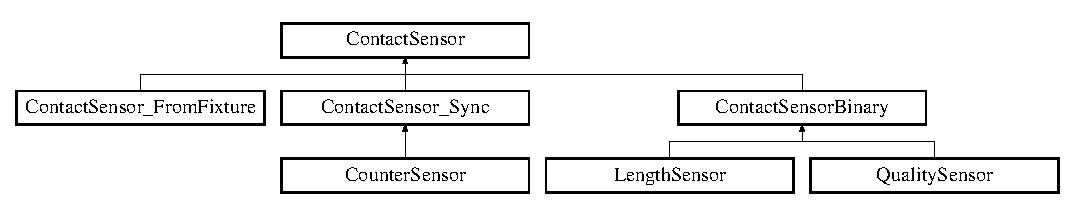
\includegraphics[height=2.359551cm]{classContactSensor}
\end{center}
\end{figure}
\subsection*{Public Member Functions}
\begin{DoxyCompactItemize}
\item 
\hyperlink{classContactSensor_adf00bb183bcb37206adb5c036e1ad3c6}{Contact\-Sensor} ()
\item 
virtual \hyperlink{classContactSensor_a460963ef5eebd0100d404f64a32149e5}{$\sim$\-Contact\-Sensor} ()
\item 
virtual int \hyperlink{classContactSensor_a14992f0e2aef3d04eca7b27bd2b2d10b}{get\-Id} ()
\item 
virtual string \hyperlink{classContactSensor_ad3f3a4b786f7d6f23caac69374dff999}{get\-Name} ()
\item 
virtual void \hyperlink{classContactSensor_ae08a9a4b2e44ec4ab2a33a482d4d286d}{draw\-Label} ()
\item 
virtual signed int \hyperlink{classContactSensor_af616ebea2da4d9fd0dacdf71eb8b32d9}{get} ()
\item 
virtual \hyperlink{Sensors_8h_a4e6d557e949865ee922fadfafd5ed0ba}{t\-\_\-sensor\-Type} \hyperlink{classContactSensor_a3ba841014a5fdaf313b555527f46595e}{get\-Type} ()
\end{DoxyCompactItemize}
\subsection*{Public Attributes}
\begin{DoxyCompactItemize}
\item 
int32 \hyperlink{classContactSensor_a589d2cd988b8d36a339394688d892df7}{m\-\_\-id}
\item 
b2\-Color \hyperlink{classContactSensor_aad27d7430ca3e8eed90f2b8b2ad849a0}{m\-\_\-color}
\item 
string \hyperlink{classContactSensor_a2cf99d03fe5bbe0773deae4a8edc4069}{m\-\_\-name}
\item 
b2\-Vec2 \hyperlink{classContactSensor_a43e68faeea764d1853eadea254ff1243}{m\-\_\-position}
\item 
float32 \hyperlink{classContactSensor_a84888f5dcbd630bd540ef314f3a22788}{m\-\_\-radius}
\item 
b2\-World $\ast$ \hyperlink{classContactSensor_a9822df2b2841440f6b5df422b017a239}{m\-\_\-world}
\item 
b2\-Body $\ast$ \hyperlink{classContactSensor_a654138f53967d7e8032f400d0e338bf5}{m\-\_\-body}
\item 
b2\-Fixture $\ast$ \hyperlink{classContactSensor_a03f59d947407b58ebce06fb3a3490633}{m\-\_\-fixture}
\item 
bool \hyperlink{classContactSensor_a79763d691af5d562d9039bfef94701b3}{m\-\_\-activated}
\item 
b2\-Body\-Def \hyperlink{classContactSensor_add4009daee3f48e71b16f6e66bdb8b32}{m\-\_\-bd}
\item 
b2\-Fixture\-Def \hyperlink{classContactSensor_a1bdedd0c81bdea57ab917320dbd9b8f2}{m\-\_\-fd}
\item 
\hyperlink{Sensors_8h_a4e6d557e949865ee922fadfafd5ed0ba}{t\-\_\-sensor\-Type} \hyperlink{classContactSensor_a9249ca2f4872b431a7c78e1fba9ccb4a}{m\-\_\-sensor\-Type}
\end{DoxyCompactItemize}


\subsection{Detailed Description}
Abstract class that other sensors inherit from. 

\subsection{Constructor \& Destructor Documentation}
\hypertarget{classContactSensor_adf00bb183bcb37206adb5c036e1ad3c6}{\index{Contact\-Sensor@{Contact\-Sensor}!Contact\-Sensor@{Contact\-Sensor}}
\index{Contact\-Sensor@{Contact\-Sensor}!ContactSensor@{Contact\-Sensor}}
\subsubsection[{Contact\-Sensor}]{\setlength{\rightskip}{0pt plus 5cm}Contact\-Sensor\-::\-Contact\-Sensor (
\begin{DoxyParamCaption}
{}
\end{DoxyParamCaption}
)}}\label{classContactSensor_adf00bb183bcb37206adb5c036e1ad3c6}
\hypertarget{classContactSensor_a460963ef5eebd0100d404f64a32149e5}{\index{Contact\-Sensor@{Contact\-Sensor}!$\sim$\-Contact\-Sensor@{$\sim$\-Contact\-Sensor}}
\index{$\sim$\-Contact\-Sensor@{$\sim$\-Contact\-Sensor}!ContactSensor@{Contact\-Sensor}}
\subsubsection[{$\sim$\-Contact\-Sensor}]{\setlength{\rightskip}{0pt plus 5cm}virtual Contact\-Sensor\-::$\sim$\-Contact\-Sensor (
\begin{DoxyParamCaption}
{}
\end{DoxyParamCaption}
)\hspace{0.3cm}{\ttfamily [inline]}, {\ttfamily [virtual]}}}\label{classContactSensor_a460963ef5eebd0100d404f64a32149e5}


\subsection{Member Function Documentation}
\hypertarget{classContactSensor_ae08a9a4b2e44ec4ab2a33a482d4d286d}{\index{Contact\-Sensor@{Contact\-Sensor}!draw\-Label@{draw\-Label}}
\index{draw\-Label@{draw\-Label}!ContactSensor@{Contact\-Sensor}}
\subsubsection[{draw\-Label}]{\setlength{\rightskip}{0pt plus 5cm}virtual void Contact\-Sensor\-::draw\-Label (
\begin{DoxyParamCaption}
{}
\end{DoxyParamCaption}
)\hspace{0.3cm}{\ttfamily [inline]}, {\ttfamily [virtual]}}}\label{classContactSensor_ae08a9a4b2e44ec4ab2a33a482d4d286d}


Reimplemented in \hyperlink{classCounterSensor_a43e99153ba1e398d66bdc1b1f5bc349d}{Counter\-Sensor}, \hyperlink{classContactSensorBinary_af6da2c72cf9ae64a27132bb9c6ba7ff3}{Contact\-Sensor\-Binary}, \hyperlink{classContactSensor__Sync_ae7eed2d2ee0e58940426d4701f695481}{Contact\-Sensor\-\_\-\-Sync}, and \hyperlink{classContactSensor__FromFixture_ab022c55f6ffa92709062d4be3a6c584b}{Contact\-Sensor\-\_\-\-From\-Fixture}.

\hypertarget{classContactSensor_af616ebea2da4d9fd0dacdf71eb8b32d9}{\index{Contact\-Sensor@{Contact\-Sensor}!get@{get}}
\index{get@{get}!ContactSensor@{Contact\-Sensor}}
\subsubsection[{get}]{\setlength{\rightskip}{0pt plus 5cm}virtual signed int Contact\-Sensor\-::get (
\begin{DoxyParamCaption}
{}
\end{DoxyParamCaption}
)\hspace{0.3cm}{\ttfamily [inline]}, {\ttfamily [virtual]}}}\label{classContactSensor_af616ebea2da4d9fd0dacdf71eb8b32d9}


Reimplemented in \hyperlink{classCounterSensor_aec52d1f6a0e52eaa61d356d9f15b665a}{Counter\-Sensor}, \hyperlink{classQualitySensor_ab8740e275a34b860b0b370183eb4d578}{Quality\-Sensor}, \hyperlink{classLengthSensor_a90d9ddfdeb189991d274026af6ab8681}{Length\-Sensor}, \hyperlink{classContactSensorBinary_a68e856e0d580f91f518099874f8c226b}{Contact\-Sensor\-Binary}, and \hyperlink{classContactSensor__FromFixture_a565839762b4c6bff70f3d7d959813580}{Contact\-Sensor\-\_\-\-From\-Fixture}.

\hypertarget{classContactSensor_a14992f0e2aef3d04eca7b27bd2b2d10b}{\index{Contact\-Sensor@{Contact\-Sensor}!get\-Id@{get\-Id}}
\index{get\-Id@{get\-Id}!ContactSensor@{Contact\-Sensor}}
\subsubsection[{get\-Id}]{\setlength{\rightskip}{0pt plus 5cm}virtual int Contact\-Sensor\-::get\-Id (
\begin{DoxyParamCaption}
{}
\end{DoxyParamCaption}
)\hspace{0.3cm}{\ttfamily [inline]}, {\ttfamily [virtual]}}}\label{classContactSensor_a14992f0e2aef3d04eca7b27bd2b2d10b}
\hypertarget{classContactSensor_ad3f3a4b786f7d6f23caac69374dff999}{\index{Contact\-Sensor@{Contact\-Sensor}!get\-Name@{get\-Name}}
\index{get\-Name@{get\-Name}!ContactSensor@{Contact\-Sensor}}
\subsubsection[{get\-Name}]{\setlength{\rightskip}{0pt plus 5cm}virtual string Contact\-Sensor\-::get\-Name (
\begin{DoxyParamCaption}
{}
\end{DoxyParamCaption}
)\hspace{0.3cm}{\ttfamily [inline]}, {\ttfamily [virtual]}}}\label{classContactSensor_ad3f3a4b786f7d6f23caac69374dff999}
\hypertarget{classContactSensor_a3ba841014a5fdaf313b555527f46595e}{\index{Contact\-Sensor@{Contact\-Sensor}!get\-Type@{get\-Type}}
\index{get\-Type@{get\-Type}!ContactSensor@{Contact\-Sensor}}
\subsubsection[{get\-Type}]{\setlength{\rightskip}{0pt plus 5cm}virtual {\bf t\-\_\-sensor\-Type} Contact\-Sensor\-::get\-Type (
\begin{DoxyParamCaption}
{}
\end{DoxyParamCaption}
)\hspace{0.3cm}{\ttfamily [inline]}, {\ttfamily [virtual]}}}\label{classContactSensor_a3ba841014a5fdaf313b555527f46595e}


\subsection{Member Data Documentation}
\hypertarget{classContactSensor_a79763d691af5d562d9039bfef94701b3}{\index{Contact\-Sensor@{Contact\-Sensor}!m\-\_\-activated@{m\-\_\-activated}}
\index{m\-\_\-activated@{m\-\_\-activated}!ContactSensor@{Contact\-Sensor}}
\subsubsection[{m\-\_\-activated}]{\setlength{\rightskip}{0pt plus 5cm}bool Contact\-Sensor\-::m\-\_\-activated}}\label{classContactSensor_a79763d691af5d562d9039bfef94701b3}
\hypertarget{classContactSensor_add4009daee3f48e71b16f6e66bdb8b32}{\index{Contact\-Sensor@{Contact\-Sensor}!m\-\_\-bd@{m\-\_\-bd}}
\index{m\-\_\-bd@{m\-\_\-bd}!ContactSensor@{Contact\-Sensor}}
\subsubsection[{m\-\_\-bd}]{\setlength{\rightskip}{0pt plus 5cm}b2\-Body\-Def Contact\-Sensor\-::m\-\_\-bd}}\label{classContactSensor_add4009daee3f48e71b16f6e66bdb8b32}
\hypertarget{classContactSensor_a654138f53967d7e8032f400d0e338bf5}{\index{Contact\-Sensor@{Contact\-Sensor}!m\-\_\-body@{m\-\_\-body}}
\index{m\-\_\-body@{m\-\_\-body}!ContactSensor@{Contact\-Sensor}}
\subsubsection[{m\-\_\-body}]{\setlength{\rightskip}{0pt plus 5cm}b2\-Body$\ast$ Contact\-Sensor\-::m\-\_\-body}}\label{classContactSensor_a654138f53967d7e8032f400d0e338bf5}
\hypertarget{classContactSensor_aad27d7430ca3e8eed90f2b8b2ad849a0}{\index{Contact\-Sensor@{Contact\-Sensor}!m\-\_\-color@{m\-\_\-color}}
\index{m\-\_\-color@{m\-\_\-color}!ContactSensor@{Contact\-Sensor}}
\subsubsection[{m\-\_\-color}]{\setlength{\rightskip}{0pt plus 5cm}b2\-Color Contact\-Sensor\-::m\-\_\-color}}\label{classContactSensor_aad27d7430ca3e8eed90f2b8b2ad849a0}
\hypertarget{classContactSensor_a1bdedd0c81bdea57ab917320dbd9b8f2}{\index{Contact\-Sensor@{Contact\-Sensor}!m\-\_\-fd@{m\-\_\-fd}}
\index{m\-\_\-fd@{m\-\_\-fd}!ContactSensor@{Contact\-Sensor}}
\subsubsection[{m\-\_\-fd}]{\setlength{\rightskip}{0pt plus 5cm}b2\-Fixture\-Def Contact\-Sensor\-::m\-\_\-fd}}\label{classContactSensor_a1bdedd0c81bdea57ab917320dbd9b8f2}
\hypertarget{classContactSensor_a03f59d947407b58ebce06fb3a3490633}{\index{Contact\-Sensor@{Contact\-Sensor}!m\-\_\-fixture@{m\-\_\-fixture}}
\index{m\-\_\-fixture@{m\-\_\-fixture}!ContactSensor@{Contact\-Sensor}}
\subsubsection[{m\-\_\-fixture}]{\setlength{\rightskip}{0pt plus 5cm}b2\-Fixture$\ast$ Contact\-Sensor\-::m\-\_\-fixture}}\label{classContactSensor_a03f59d947407b58ebce06fb3a3490633}
\hypertarget{classContactSensor_a589d2cd988b8d36a339394688d892df7}{\index{Contact\-Sensor@{Contact\-Sensor}!m\-\_\-id@{m\-\_\-id}}
\index{m\-\_\-id@{m\-\_\-id}!ContactSensor@{Contact\-Sensor}}
\subsubsection[{m\-\_\-id}]{\setlength{\rightskip}{0pt plus 5cm}int32 Contact\-Sensor\-::m\-\_\-id}}\label{classContactSensor_a589d2cd988b8d36a339394688d892df7}
\hypertarget{classContactSensor_a2cf99d03fe5bbe0773deae4a8edc4069}{\index{Contact\-Sensor@{Contact\-Sensor}!m\-\_\-name@{m\-\_\-name}}
\index{m\-\_\-name@{m\-\_\-name}!ContactSensor@{Contact\-Sensor}}
\subsubsection[{m\-\_\-name}]{\setlength{\rightskip}{0pt plus 5cm}string Contact\-Sensor\-::m\-\_\-name}}\label{classContactSensor_a2cf99d03fe5bbe0773deae4a8edc4069}
\hypertarget{classContactSensor_a43e68faeea764d1853eadea254ff1243}{\index{Contact\-Sensor@{Contact\-Sensor}!m\-\_\-position@{m\-\_\-position}}
\index{m\-\_\-position@{m\-\_\-position}!ContactSensor@{Contact\-Sensor}}
\subsubsection[{m\-\_\-position}]{\setlength{\rightskip}{0pt plus 5cm}b2\-Vec2 Contact\-Sensor\-::m\-\_\-position}}\label{classContactSensor_a43e68faeea764d1853eadea254ff1243}
\hypertarget{classContactSensor_a84888f5dcbd630bd540ef314f3a22788}{\index{Contact\-Sensor@{Contact\-Sensor}!m\-\_\-radius@{m\-\_\-radius}}
\index{m\-\_\-radius@{m\-\_\-radius}!ContactSensor@{Contact\-Sensor}}
\subsubsection[{m\-\_\-radius}]{\setlength{\rightskip}{0pt plus 5cm}float32 Contact\-Sensor\-::m\-\_\-radius}}\label{classContactSensor_a84888f5dcbd630bd540ef314f3a22788}
\hypertarget{classContactSensor_a9249ca2f4872b431a7c78e1fba9ccb4a}{\index{Contact\-Sensor@{Contact\-Sensor}!m\-\_\-sensor\-Type@{m\-\_\-sensor\-Type}}
\index{m\-\_\-sensor\-Type@{m\-\_\-sensor\-Type}!ContactSensor@{Contact\-Sensor}}
\subsubsection[{m\-\_\-sensor\-Type}]{\setlength{\rightskip}{0pt plus 5cm}{\bf t\-\_\-sensor\-Type} Contact\-Sensor\-::m\-\_\-sensor\-Type}}\label{classContactSensor_a9249ca2f4872b431a7c78e1fba9ccb4a}
\hypertarget{classContactSensor_a9822df2b2841440f6b5df422b017a239}{\index{Contact\-Sensor@{Contact\-Sensor}!m\-\_\-world@{m\-\_\-world}}
\index{m\-\_\-world@{m\-\_\-world}!ContactSensor@{Contact\-Sensor}}
\subsubsection[{m\-\_\-world}]{\setlength{\rightskip}{0pt plus 5cm}b2\-World$\ast$ Contact\-Sensor\-::m\-\_\-world}}\label{classContactSensor_a9822df2b2841440f6b5df422b017a239}


The documentation for this class was generated from the following files\-:\begin{DoxyCompactItemize}
\item 
\hyperlink{Sensors_8h}{Sensors.\-h}\item 
\hyperlink{Sensors_8cpp}{Sensors.\-cpp}\end{DoxyCompactItemize}

\hypertarget{classContactSensor__FromFixture}{\section{Contact\-Sensor\-\_\-\-From\-Fixture Class Reference}
\label{classContactSensor__FromFixture}\index{Contact\-Sensor\-\_\-\-From\-Fixture@{Contact\-Sensor\-\_\-\-From\-Fixture}}
}


Turn arbitrary Box2\-D fixture into binary sensor.  




{\ttfamily \#include $<$Sensors.\-h$>$}

Inheritance diagram for Contact\-Sensor\-\_\-\-From\-Fixture\-:\begin{figure}[H]
\begin{center}
\leavevmode
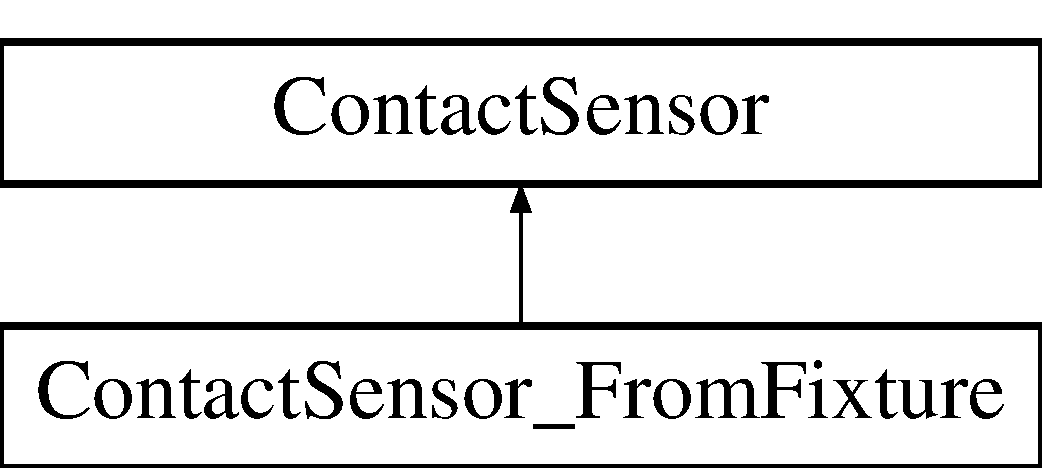
\includegraphics[height=2.000000cm]{classContactSensor__FromFixture}
\end{center}
\end{figure}
\subsection*{Public Member Functions}
\begin{DoxyCompactItemize}
\item 
\hyperlink{classContactSensor__FromFixture_a9989b5549cef639368089acfe5dcdfe6}{Contact\-Sensor\-\_\-\-From\-Fixture} (int id, b2\-Fixture $\ast$fixture)
\begin{DoxyCompactList}\small\item\em Turn arbitrary b2\-Fixture into binary sensor. \end{DoxyCompactList}\item 
signed int \hyperlink{classContactSensor__FromFixture_a565839762b4c6bff70f3d7d959813580}{get} ()
\begin{DoxyCompactList}\small\item\em Return sensors measured value. \end{DoxyCompactList}\item 
void \hyperlink{classContactSensor__FromFixture_ab022c55f6ffa92709062d4be3a6c584b}{draw\-Label} ()
\begin{DoxyCompactList}\small\item\em Draw sensor label. \end{DoxyCompactList}\end{DoxyCompactItemize}
\subsection*{Public Attributes}
\begin{DoxyCompactItemize}
\item 
float32 \hyperlink{classContactSensor__FromFixture_a059bda2fabb5680ff425af83274feb22}{m\-\_\-radius}
\end{DoxyCompactItemize}


\subsection{Detailed Description}
Turn arbitrary Box2\-D fixture into binary sensor. 

{\bfseries Example\-:}  To create S1 and activate the sensor, by adding it to the sensor-\/set, we write the following lines of code\-: 
\begin{DoxyCode}
\hyperlink{classContactSensor__FromFixture}{ContactSensor\_FromFixture}* liftSensor = \textcolor{keyword}{new} 
      \hyperlink{classContactSensor__FromFixture_a9989b5549cef639368089acfe5dcdfe6}{ContactSensor\_FromFixture}(1,packageInput->
      getLiftSensorFixture());
m\_sensorSet->add(liftSensor);
\end{DoxyCode}
 

\subsection{Constructor \& Destructor Documentation}
\hypertarget{classContactSensor__FromFixture_a9989b5549cef639368089acfe5dcdfe6}{\index{Contact\-Sensor\-\_\-\-From\-Fixture@{Contact\-Sensor\-\_\-\-From\-Fixture}!Contact\-Sensor\-\_\-\-From\-Fixture@{Contact\-Sensor\-\_\-\-From\-Fixture}}
\index{Contact\-Sensor\-\_\-\-From\-Fixture@{Contact\-Sensor\-\_\-\-From\-Fixture}!ContactSensor_FromFixture@{Contact\-Sensor\-\_\-\-From\-Fixture}}
\subsubsection[{Contact\-Sensor\-\_\-\-From\-Fixture}]{\setlength{\rightskip}{0pt plus 5cm}Contact\-Sensor\-\_\-\-From\-Fixture\-::\-Contact\-Sensor\-\_\-\-From\-Fixture (
\begin{DoxyParamCaption}
\item[{int}]{id, }
\item[{b2\-Fixture $\ast$}]{fixture}
\end{DoxyParamCaption}
)}}\label{classContactSensor__FromFixture_a9989b5549cef639368089acfe5dcdfe6}


Turn arbitrary b2\-Fixture into binary sensor. 


\begin{DoxyParams}{Parameters}
{\em id} & The id of the sensor. This value will be visible as part of the sensor label. \\
\hline
{\em fixture} & Pointer to the b2\-Fixture that you want to turn in to a sensor. \\
\hline
\end{DoxyParams}


\subsection{Member Function Documentation}
\hypertarget{classContactSensor__FromFixture_ab022c55f6ffa92709062d4be3a6c584b}{\index{Contact\-Sensor\-\_\-\-From\-Fixture@{Contact\-Sensor\-\_\-\-From\-Fixture}!draw\-Label@{draw\-Label}}
\index{draw\-Label@{draw\-Label}!ContactSensor_FromFixture@{Contact\-Sensor\-\_\-\-From\-Fixture}}
\subsubsection[{draw\-Label}]{\setlength{\rightskip}{0pt plus 5cm}void Contact\-Sensor\-\_\-\-From\-Fixture\-::draw\-Label (
\begin{DoxyParamCaption}
{}
\end{DoxyParamCaption}
)\hspace{0.3cm}{\ttfamily [virtual]}}}\label{classContactSensor__FromFixture_ab022c55f6ffa92709062d4be3a6c584b}


Draw sensor label. 



Reimplemented from \hyperlink{classContactSensor_ae08a9a4b2e44ec4ab2a33a482d4d286d}{Contact\-Sensor}.

\hypertarget{classContactSensor__FromFixture_a565839762b4c6bff70f3d7d959813580}{\index{Contact\-Sensor\-\_\-\-From\-Fixture@{Contact\-Sensor\-\_\-\-From\-Fixture}!get@{get}}
\index{get@{get}!ContactSensor_FromFixture@{Contact\-Sensor\-\_\-\-From\-Fixture}}
\subsubsection[{get}]{\setlength{\rightskip}{0pt plus 5cm}signed int Contact\-Sensor\-\_\-\-From\-Fixture\-::get (
\begin{DoxyParamCaption}
{}
\end{DoxyParamCaption}
)\hspace{0.3cm}{\ttfamily [virtual]}}}\label{classContactSensor__FromFixture_a565839762b4c6bff70f3d7d959813580}


Return sensors measured value. 



Reimplemented from \hyperlink{classContactSensor_af616ebea2da4d9fd0dacdf71eb8b32d9}{Contact\-Sensor}.



\subsection{Member Data Documentation}
\hypertarget{classContactSensor__FromFixture_a059bda2fabb5680ff425af83274feb22}{\index{Contact\-Sensor\-\_\-\-From\-Fixture@{Contact\-Sensor\-\_\-\-From\-Fixture}!m\-\_\-radius@{m\-\_\-radius}}
\index{m\-\_\-radius@{m\-\_\-radius}!ContactSensor_FromFixture@{Contact\-Sensor\-\_\-\-From\-Fixture}}
\subsubsection[{m\-\_\-radius}]{\setlength{\rightskip}{0pt plus 5cm}float32 Contact\-Sensor\-\_\-\-From\-Fixture\-::m\-\_\-radius}}\label{classContactSensor__FromFixture_a059bda2fabb5680ff425af83274feb22}


The documentation for this class was generated from the following files\-:\begin{DoxyCompactItemize}
\item 
\hyperlink{Sensors_8h}{Sensors.\-h}\item 
\hyperlink{Sensors_8cpp}{Sensors.\-cpp}\end{DoxyCompactItemize}

\hypertarget{classContactSensor__Sync}{\section{Contact\-Sensor\-\_\-\-Sync Class Reference}
\label{classContactSensor__Sync}\index{Contact\-Sensor\-\_\-\-Sync@{Contact\-Sensor\-\_\-\-Sync}}
}


Used by the \hyperlink{classConveyorSynchronizer}{Conveyor\-Synchronizer}.  




{\ttfamily \#include $<$Sensors.\-h$>$}

Inheritance diagram for Contact\-Sensor\-\_\-\-Sync\-:\begin{figure}[H]
\begin{center}
\leavevmode
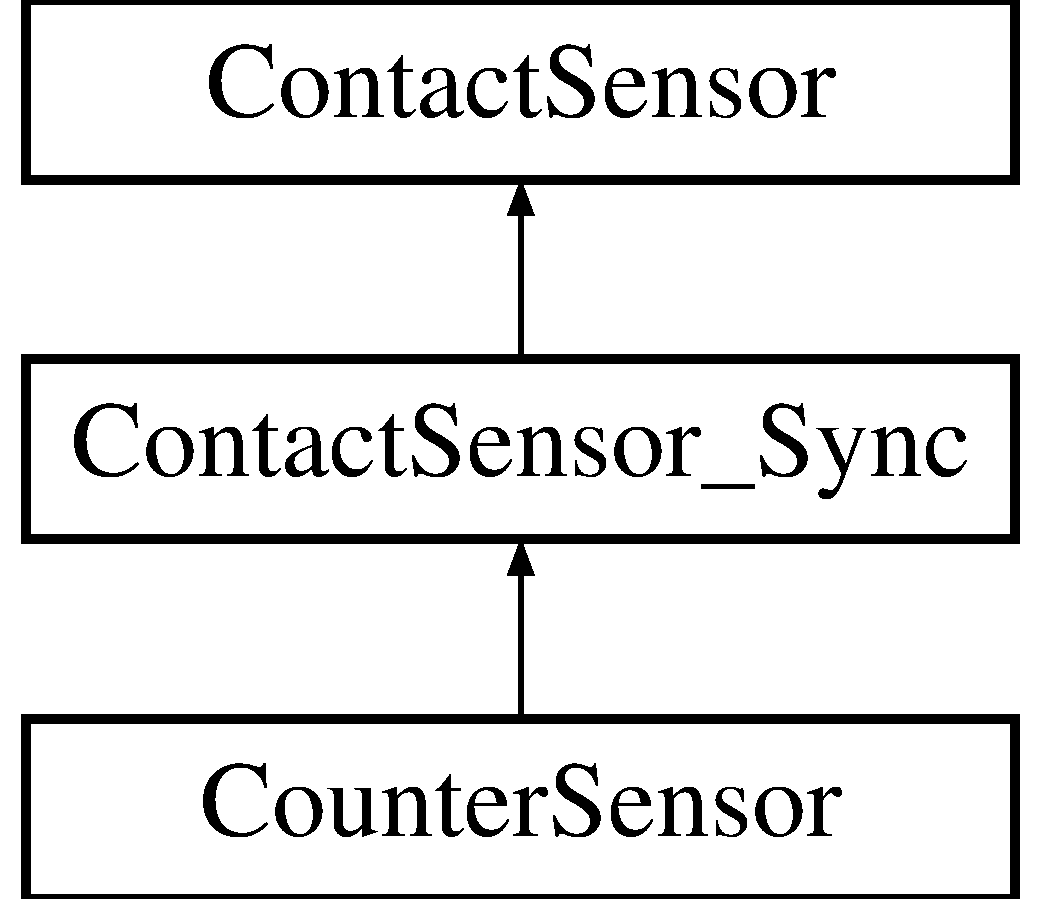
\includegraphics[height=3.000000cm]{classContactSensor__Sync}
\end{center}
\end{figure}
\subsection*{Public Member Functions}
\begin{DoxyCompactItemize}
\item 
\hyperlink{classContactSensor__Sync_a3067639c78a7f5e01724f15bdf023026}{Contact\-Sensor\-\_\-\-Sync} (b2\-Vec2 position, float32 radius, b2\-Filter filter, b2\-World $\ast$world)
\begin{DoxyCompactList}\small\item\em Constructs a synchronization-\/sensor. \end{DoxyCompactList}\item 
virtual void \hyperlink{classContactSensor__Sync_ae7eed2d2ee0e58940426d4701f695481}{draw\-Label} ()
\begin{DoxyCompactList}\small\item\em Draw \char`\"{}sync\char`\"{} in red next to the sensor. \end{DoxyCompactList}\end{DoxyCompactItemize}
\subsection*{Public Attributes}
\begin{DoxyCompactItemize}
\item 
float32 \hyperlink{classContactSensor__Sync_ad744459b1b2dc3836a5f8a68a8f9ad38}{m\-\_\-radius}
\end{DoxyCompactItemize}


\subsection{Detailed Description}
Used by the \hyperlink{classConveyorSynchronizer}{Conveyor\-Synchronizer}. 

Each \hyperlink{classConveyor}{Conveyor} has one of these sensors. If a \hyperlink{classConveyor}{Conveyor} is registered with a \hyperlink{classConveyorSynchronizer}{Conveyor\-Synchronizer} a label with the text {\bfseries sync} will show up next to the sensor\-:

 

\subsection{Constructor \& Destructor Documentation}
\hypertarget{classContactSensor__Sync_a3067639c78a7f5e01724f15bdf023026}{\index{Contact\-Sensor\-\_\-\-Sync@{Contact\-Sensor\-\_\-\-Sync}!Contact\-Sensor\-\_\-\-Sync@{Contact\-Sensor\-\_\-\-Sync}}
\index{Contact\-Sensor\-\_\-\-Sync@{Contact\-Sensor\-\_\-\-Sync}!ContactSensor_Sync@{Contact\-Sensor\-\_\-\-Sync}}
\subsubsection[{Contact\-Sensor\-\_\-\-Sync}]{\setlength{\rightskip}{0pt plus 5cm}Contact\-Sensor\-\_\-\-Sync\-::\-Contact\-Sensor\-\_\-\-Sync (
\begin{DoxyParamCaption}
\item[{b2\-Vec2}]{position, }
\item[{float32}]{radius, }
\item[{b2\-Filter}]{filter, }
\item[{b2\-World $\ast$}]{world}
\end{DoxyParamCaption}
)}}\label{classContactSensor__Sync_a3067639c78a7f5e01724f15bdf023026}


Constructs a synchronization-\/sensor. 


\begin{DoxyParams}{Parameters}
{\em position} & The position of the sensors circular shaped fixture. \\
\hline
{\em radius} & The radius of the sensors fixture. \\
\hline
{\em filter} & The sensors filter is used to control what sensors collide with she sensors fixture. \\
\hline
{\em world} & Pointer to the world in which you want to create the sensor. \\
\hline
\end{DoxyParams}


\subsection{Member Function Documentation}
\hypertarget{classContactSensor__Sync_ae7eed2d2ee0e58940426d4701f695481}{\index{Contact\-Sensor\-\_\-\-Sync@{Contact\-Sensor\-\_\-\-Sync}!draw\-Label@{draw\-Label}}
\index{draw\-Label@{draw\-Label}!ContactSensor_Sync@{Contact\-Sensor\-\_\-\-Sync}}
\subsubsection[{draw\-Label}]{\setlength{\rightskip}{0pt plus 5cm}void Contact\-Sensor\-\_\-\-Sync\-::draw\-Label (
\begin{DoxyParamCaption}
{}
\end{DoxyParamCaption}
)\hspace{0.3cm}{\ttfamily [virtual]}}}\label{classContactSensor__Sync_ae7eed2d2ee0e58940426d4701f695481}


Draw \char`\"{}sync\char`\"{} in red next to the sensor. 



Reimplemented from \hyperlink{classContactSensor_ae08a9a4b2e44ec4ab2a33a482d4d286d}{Contact\-Sensor}.



Reimplemented in \hyperlink{classCounterSensor_a43e99153ba1e398d66bdc1b1f5bc349d}{Counter\-Sensor}.



\subsection{Member Data Documentation}
\hypertarget{classContactSensor__Sync_ad744459b1b2dc3836a5f8a68a8f9ad38}{\index{Contact\-Sensor\-\_\-\-Sync@{Contact\-Sensor\-\_\-\-Sync}!m\-\_\-radius@{m\-\_\-radius}}
\index{m\-\_\-radius@{m\-\_\-radius}!ContactSensor_Sync@{Contact\-Sensor\-\_\-\-Sync}}
\subsubsection[{m\-\_\-radius}]{\setlength{\rightskip}{0pt plus 5cm}float32 Contact\-Sensor\-\_\-\-Sync\-::m\-\_\-radius}}\label{classContactSensor__Sync_ad744459b1b2dc3836a5f8a68a8f9ad38}


The documentation for this class was generated from the following files\-:\begin{DoxyCompactItemize}
\item 
\hyperlink{Sensors_8h}{Sensors.\-h}\item 
\hyperlink{Sensors_8cpp}{Sensors.\-cpp}\end{DoxyCompactItemize}

\hypertarget{classContactSensorBinary}{\section{Contact\-Sensor\-Binary Class Reference}
\label{classContactSensorBinary}\index{Contact\-Sensor\-Binary@{Contact\-Sensor\-Binary}}
}


This sensor is circular shaped and has only two states, O\-N and O\-Ff.  




{\ttfamily \#include $<$Sensors.\-h$>$}

Inheritance diagram for Contact\-Sensor\-Binary\-:\begin{figure}[H]
\begin{center}
\leavevmode
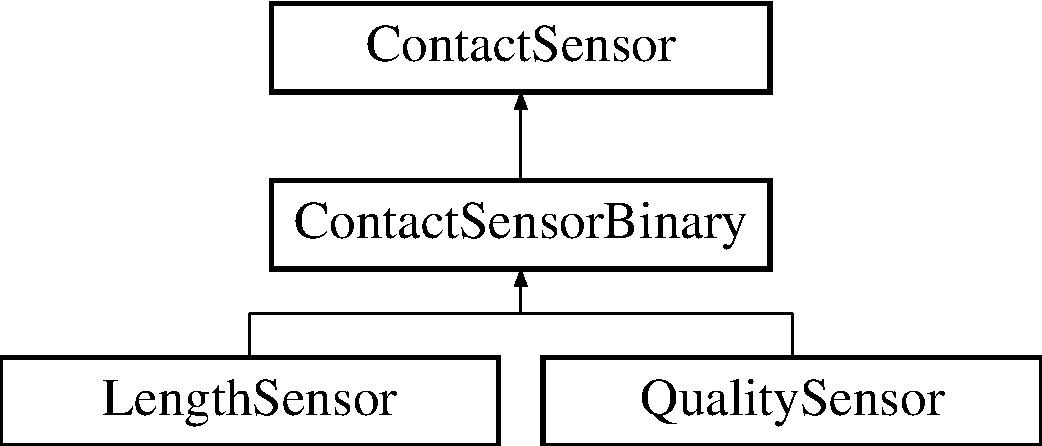
\includegraphics[height=3.000000cm]{classContactSensorBinary}
\end{center}
\end{figure}
\subsection*{Public Member Functions}
\begin{DoxyCompactItemize}
\item 
\hyperlink{classContactSensorBinary_acc94779d598ff1e435bc8726657c65af}{Contact\-Sensor\-Binary} (int id, b2\-Vec2 position, float32 radius, b2\-World $\ast$world)
\item 
virtual void \hyperlink{classContactSensorBinary_af6da2c72cf9ae64a27132bb9c6ba7ff3}{draw\-Label} ()
\item 
virtual signed int \hyperlink{classContactSensorBinary_a68e856e0d580f91f518099874f8c226b}{get} ()
\begin{DoxyCompactList}\small\item\em Return the state of the sensor. \end{DoxyCompactList}\end{DoxyCompactItemize}
\subsection*{Public Attributes}
\begin{DoxyCompactItemize}
\item 
float32 \hyperlink{classContactSensorBinary_a0670dd47fe23d52cc4d9dfccddb3bcab}{m\-\_\-radius}
\end{DoxyCompactItemize}


\subsection{Detailed Description}
This sensor is circular shaped and has only two states, O\-N and O\-Ff. 

\subsection{Constructor \& Destructor Documentation}
\hypertarget{classContactSensorBinary_acc94779d598ff1e435bc8726657c65af}{\index{Contact\-Sensor\-Binary@{Contact\-Sensor\-Binary}!Contact\-Sensor\-Binary@{Contact\-Sensor\-Binary}}
\index{Contact\-Sensor\-Binary@{Contact\-Sensor\-Binary}!ContactSensorBinary@{Contact\-Sensor\-Binary}}
\subsubsection[{Contact\-Sensor\-Binary}]{\setlength{\rightskip}{0pt plus 5cm}Contact\-Sensor\-Binary\-::\-Contact\-Sensor\-Binary (
\begin{DoxyParamCaption}
\item[{int}]{id, }
\item[{b2\-Vec2}]{position, }
\item[{float32}]{radius, }
\item[{b2\-World $\ast$}]{world}
\end{DoxyParamCaption}
)}}\label{classContactSensorBinary_acc94779d598ff1e435bc8726657c65af}


\subsection{Member Function Documentation}
\hypertarget{classContactSensorBinary_af6da2c72cf9ae64a27132bb9c6ba7ff3}{\index{Contact\-Sensor\-Binary@{Contact\-Sensor\-Binary}!draw\-Label@{draw\-Label}}
\index{draw\-Label@{draw\-Label}!ContactSensorBinary@{Contact\-Sensor\-Binary}}
\subsubsection[{draw\-Label}]{\setlength{\rightskip}{0pt plus 5cm}void Contact\-Sensor\-Binary\-::draw\-Label (
\begin{DoxyParamCaption}
{}
\end{DoxyParamCaption}
)\hspace{0.3cm}{\ttfamily [virtual]}}}\label{classContactSensorBinary_af6da2c72cf9ae64a27132bb9c6ba7ff3}


Reimplemented from \hyperlink{classContactSensor_ae08a9a4b2e44ec4ab2a33a482d4d286d}{Contact\-Sensor}.

\hypertarget{classContactSensorBinary_a68e856e0d580f91f518099874f8c226b}{\index{Contact\-Sensor\-Binary@{Contact\-Sensor\-Binary}!get@{get}}
\index{get@{get}!ContactSensorBinary@{Contact\-Sensor\-Binary}}
\subsubsection[{get}]{\setlength{\rightskip}{0pt plus 5cm}signed int Contact\-Sensor\-Binary\-::get (
\begin{DoxyParamCaption}
{}
\end{DoxyParamCaption}
)\hspace{0.3cm}{\ttfamily [virtual]}}}\label{classContactSensorBinary_a68e856e0d580f91f518099874f8c226b}


Return the state of the sensor. 



Reimplemented from \hyperlink{classContactSensor_af616ebea2da4d9fd0dacdf71eb8b32d9}{Contact\-Sensor}.



Reimplemented in \hyperlink{classQualitySensor_ab8740e275a34b860b0b370183eb4d578}{Quality\-Sensor}, and \hyperlink{classLengthSensor_a90d9ddfdeb189991d274026af6ab8681}{Length\-Sensor}.



\subsection{Member Data Documentation}
\hypertarget{classContactSensorBinary_a0670dd47fe23d52cc4d9dfccddb3bcab}{\index{Contact\-Sensor\-Binary@{Contact\-Sensor\-Binary}!m\-\_\-radius@{m\-\_\-radius}}
\index{m\-\_\-radius@{m\-\_\-radius}!ContactSensorBinary@{Contact\-Sensor\-Binary}}
\subsubsection[{m\-\_\-radius}]{\setlength{\rightskip}{0pt plus 5cm}float32 Contact\-Sensor\-Binary\-::m\-\_\-radius}}\label{classContactSensorBinary_a0670dd47fe23d52cc4d9dfccddb3bcab}


The documentation for this class was generated from the following files\-:\begin{DoxyCompactItemize}
\item 
\hyperlink{Sensors_8h}{Sensors.\-h}\item 
\hyperlink{Sensors_8cpp}{Sensors.\-cpp}\end{DoxyCompactItemize}

\hypertarget{classConveyor}{\section{Conveyor Class Reference}
\label{classConveyor}\index{Conveyor@{Conveyor}}
}


Assemble the conveyor and expose an interface through which controlling the conveyor is possible.  




{\ttfamily \#include $<$Conveyor.\-h$>$}

\subsection*{Public Member Functions}
\begin{DoxyCompactItemize}
\item 
\hyperlink{classConveyor_a49aeaaa057ce5bbce9d0dbd8efcd86cf}{Conveyor} (b2\-Vec2 p1, b2\-Vec2 p2, float32 beam\-Thickness, float32 belt\-Thickness, int N, int M, \hyperlink{Conveyor_8h_a98261db3679be2885c0bdad13c27d7b1}{t\-\_\-medbringer\-Type} medbringer\-Type, int sensor\-Pos, float32 sensor\-Adjustment, int cm\-Bits, b2\-World $\ast$world)
\item 
void \hyperlink{classConveyor_a2c161757c96058a1af3225192db4add6}{set\-Speed} (float32 speed)
\begin{DoxyCompactList}\small\item\em Set the speed of the conveyorbelt. \end{DoxyCompactList}\item 
void \hyperlink{classConveyor_a85ac6c349c3a15e57279c5138da2cfed}{pause} ()
\begin{DoxyCompactList}\small\item\em Pause the conveyor. \end{DoxyCompactList}\item 
void \hyperlink{classConveyor_a50cae15e0bb0f744297ce51651ad26f2}{play} ()
\begin{DoxyCompactList}\small\item\em Run the conveyor. \end{DoxyCompactList}\item 
bool \hyperlink{classConveyor_a3d97165f61dd8b1f1d27214dce8383df}{is\-Paused} ()
\begin{DoxyCompactList}\small\item\em Check if conveyor is paused. \end{DoxyCompactList}\item 
void \hyperlink{classConveyor_a37bd6265284a18cc7dd5247f2367b485}{run} ()
\begin{DoxyCompactList}\small\item\em You need to call this function iteratively. \end{DoxyCompactList}\item 
\hyperlink{classWheel}{Wheel} $\ast$ \hyperlink{classConveyor_ae742b2ae2f99c1d3f467ba8718b822f2}{get\-Wheel1} () const 
\item 
\hyperlink{classWheel}{Wheel} $\ast$ \hyperlink{classConveyor_a04fcab5fd72b64c1d05db0a8b1dfc597}{get\-Wheel2} () const 
\item 
\hyperlink{classContactSensor}{Contact\-Sensor} $\ast$ \hyperlink{classConveyor_ac9402d02e1d79aa5faebcb229c45620a}{get\-Sensor} ()
\begin{DoxyCompactList}\small\item\em Return the synchronization-\/sensor. \end{DoxyCompactList}\item 
bool \hyperlink{classConveyor_a475ce9af7f0d6c108763728228e32b56}{is\-Sensor\-Activated} ()
\begin{DoxyCompactList}\small\item\em Check state of synchronization-\/sensor. \end{DoxyCompactList}\end{DoxyCompactItemize}
\subsection*{Public Attributes}
\begin{DoxyCompactItemize}
\item 
\hyperlink{classWheel}{Wheel} $\ast$ \hyperlink{classConveyor_add4c93f9cde9efd141ec813e429161b3}{m\-\_\-wheel1}
\item 
\hyperlink{classWheel}{Wheel} $\ast$ \hyperlink{classConveyor_a49272a7a68a6d1072c170fe4080c720b}{m\-\_\-wheel2}
\item 
b2\-Vec2 \hyperlink{classConveyor_a113c9d44089b1538f7c35e6888366904}{m\-\_\-p1}
\item 
b2\-Vec2 \hyperlink{classConveyor_aa1cd90bad95a21f56a56d8c468b366bf}{m\-\_\-p2}
\item 
float32 \hyperlink{classConveyor_a38e79e2c88efd24fd626485bff30f697}{m\-\_\-belt\-Thickness}
\item 
float32 \hyperlink{classConveyor_aa16886f74252de25d3d8972779f282b0}{m\-\_\-beam\-Thickness}
\item 
float32 \hyperlink{classConveyor_aada37ff91042927da34b025345c9350f}{m\-\_\-speed}
\item 
\hyperlink{classConveyorBelt}{Conveyor\-Belt} $\ast$ \hyperlink{classConveyor_aa1640f4a83793107fcb2af5915b3fba1}{m\-\_\-conveyor\-Belt}
\item 
\hyperlink{classConveyorBeltShield}{Conveyor\-Belt\-Shield} $\ast$ \hyperlink{classConveyor_acb82b369204df0d42ae4483f9e0c9374}{m\-\_\-conveyor\-Belt\-Shield}
\item 
bool \hyperlink{classConveyor_a5cf9db504e884a9542b52037e6e7eb4f}{m\-\_\-b\-Paused}
\end{DoxyCompactItemize}


\subsection{Detailed Description}
Assemble the conveyor and expose an interface through which controlling the conveyor is possible. 

\subsection{Constructor \& Destructor Documentation}
\hypertarget{classConveyor_a49aeaaa057ce5bbce9d0dbd8efcd86cf}{\index{Conveyor@{Conveyor}!Conveyor@{Conveyor}}
\index{Conveyor@{Conveyor}!Conveyor@{Conveyor}}
\subsubsection[{Conveyor}]{\setlength{\rightskip}{0pt plus 5cm}Conveyor\-::\-Conveyor (
\begin{DoxyParamCaption}
\item[{b2\-Vec2}]{p1, }
\item[{b2\-Vec2}]{p2, }
\item[{float32}]{beam\-Thickness, }
\item[{float32}]{belt\-Thickness, }
\item[{int}]{N, }
\item[{int}]{M, }
\item[{{\bf t\-\_\-medbringer\-Type}}]{medbringer\-Type, }
\item[{int}]{sensor\-Pos, }
\item[{float32}]{sensor\-Adjustment, }
\item[{int}]{cm\-Bits, }
\item[{b2\-World $\ast$}]{world}
\end{DoxyParamCaption}
)}}\label{classConveyor_a49aeaaa057ce5bbce9d0dbd8efcd86cf}


\subsection{Member Function Documentation}
\hypertarget{classConveyor_ac9402d02e1d79aa5faebcb229c45620a}{\index{Conveyor@{Conveyor}!get\-Sensor@{get\-Sensor}}
\index{get\-Sensor@{get\-Sensor}!Conveyor@{Conveyor}}
\subsubsection[{get\-Sensor}]{\setlength{\rightskip}{0pt plus 5cm}{\bf Contact\-Sensor} $\ast$ Conveyor\-::get\-Sensor (
\begin{DoxyParamCaption}
{}
\end{DoxyParamCaption}
)}}\label{classConveyor_ac9402d02e1d79aa5faebcb229c45620a}


Return the synchronization-\/sensor. 

\hypertarget{classConveyor_ae742b2ae2f99c1d3f467ba8718b822f2}{\index{Conveyor@{Conveyor}!get\-Wheel1@{get\-Wheel1}}
\index{get\-Wheel1@{get\-Wheel1}!Conveyor@{Conveyor}}
\subsubsection[{get\-Wheel1}]{\setlength{\rightskip}{0pt plus 5cm}{\bf Wheel}$\ast$ Conveyor\-::get\-Wheel1 (
\begin{DoxyParamCaption}
{}
\end{DoxyParamCaption}
) const\hspace{0.3cm}{\ttfamily [inline]}}}\label{classConveyor_ae742b2ae2f99c1d3f467ba8718b822f2}
\hypertarget{classConveyor_a04fcab5fd72b64c1d05db0a8b1dfc597}{\index{Conveyor@{Conveyor}!get\-Wheel2@{get\-Wheel2}}
\index{get\-Wheel2@{get\-Wheel2}!Conveyor@{Conveyor}}
\subsubsection[{get\-Wheel2}]{\setlength{\rightskip}{0pt plus 5cm}{\bf Wheel}$\ast$ Conveyor\-::get\-Wheel2 (
\begin{DoxyParamCaption}
{}
\end{DoxyParamCaption}
) const\hspace{0.3cm}{\ttfamily [inline]}}}\label{classConveyor_a04fcab5fd72b64c1d05db0a8b1dfc597}
\hypertarget{classConveyor_a3d97165f61dd8b1f1d27214dce8383df}{\index{Conveyor@{Conveyor}!is\-Paused@{is\-Paused}}
\index{is\-Paused@{is\-Paused}!Conveyor@{Conveyor}}
\subsubsection[{is\-Paused}]{\setlength{\rightskip}{0pt plus 5cm}bool Conveyor\-::is\-Paused (
\begin{DoxyParamCaption}
{}
\end{DoxyParamCaption}
)\hspace{0.3cm}{\ttfamily [inline]}}}\label{classConveyor_a3d97165f61dd8b1f1d27214dce8383df}


Check if conveyor is paused. 

\hypertarget{classConveyor_a475ce9af7f0d6c108763728228e32b56}{\index{Conveyor@{Conveyor}!is\-Sensor\-Activated@{is\-Sensor\-Activated}}
\index{is\-Sensor\-Activated@{is\-Sensor\-Activated}!Conveyor@{Conveyor}}
\subsubsection[{is\-Sensor\-Activated}]{\setlength{\rightskip}{0pt plus 5cm}bool Conveyor\-::is\-Sensor\-Activated (
\begin{DoxyParamCaption}
{}
\end{DoxyParamCaption}
)}}\label{classConveyor_a475ce9af7f0d6c108763728228e32b56}


Check state of synchronization-\/sensor. 

\hypertarget{classConveyor_a85ac6c349c3a15e57279c5138da2cfed}{\index{Conveyor@{Conveyor}!pause@{pause}}
\index{pause@{pause}!Conveyor@{Conveyor}}
\subsubsection[{pause}]{\setlength{\rightskip}{0pt plus 5cm}void Conveyor\-::pause (
\begin{DoxyParamCaption}
{}
\end{DoxyParamCaption}
)}}\label{classConveyor_a85ac6c349c3a15e57279c5138da2cfed}


Pause the conveyor. 

\hypertarget{classConveyor_a50cae15e0bb0f744297ce51651ad26f2}{\index{Conveyor@{Conveyor}!play@{play}}
\index{play@{play}!Conveyor@{Conveyor}}
\subsubsection[{play}]{\setlength{\rightskip}{0pt plus 5cm}void Conveyor\-::play (
\begin{DoxyParamCaption}
{}
\end{DoxyParamCaption}
)}}\label{classConveyor_a50cae15e0bb0f744297ce51651ad26f2}


Run the conveyor. 

\hypertarget{classConveyor_a37bd6265284a18cc7dd5247f2367b485}{\index{Conveyor@{Conveyor}!run@{run}}
\index{run@{run}!Conveyor@{Conveyor}}
\subsubsection[{run}]{\setlength{\rightskip}{0pt plus 5cm}void Conveyor\-::run (
\begin{DoxyParamCaption}
{}
\end{DoxyParamCaption}
)}}\label{classConveyor_a37bd6265284a18cc7dd5247f2367b485}


You need to call this function iteratively. 

\hypertarget{classConveyor_a2c161757c96058a1af3225192db4add6}{\index{Conveyor@{Conveyor}!set\-Speed@{set\-Speed}}
\index{set\-Speed@{set\-Speed}!Conveyor@{Conveyor}}
\subsubsection[{set\-Speed}]{\setlength{\rightskip}{0pt plus 5cm}void Conveyor\-::set\-Speed (
\begin{DoxyParamCaption}
\item[{float32}]{speed}
\end{DoxyParamCaption}
)}}\label{classConveyor_a2c161757c96058a1af3225192db4add6}


Set the speed of the conveyorbelt. 



\subsection{Member Data Documentation}
\hypertarget{classConveyor_aa16886f74252de25d3d8972779f282b0}{\index{Conveyor@{Conveyor}!m\-\_\-beam\-Thickness@{m\-\_\-beam\-Thickness}}
\index{m\-\_\-beam\-Thickness@{m\-\_\-beam\-Thickness}!Conveyor@{Conveyor}}
\subsubsection[{m\-\_\-beam\-Thickness}]{\setlength{\rightskip}{0pt plus 5cm}float32 Conveyor\-::m\-\_\-beam\-Thickness}}\label{classConveyor_aa16886f74252de25d3d8972779f282b0}
\hypertarget{classConveyor_a38e79e2c88efd24fd626485bff30f697}{\index{Conveyor@{Conveyor}!m\-\_\-belt\-Thickness@{m\-\_\-belt\-Thickness}}
\index{m\-\_\-belt\-Thickness@{m\-\_\-belt\-Thickness}!Conveyor@{Conveyor}}
\subsubsection[{m\-\_\-belt\-Thickness}]{\setlength{\rightskip}{0pt plus 5cm}float32 Conveyor\-::m\-\_\-belt\-Thickness}}\label{classConveyor_a38e79e2c88efd24fd626485bff30f697}
\hypertarget{classConveyor_a5cf9db504e884a9542b52037e6e7eb4f}{\index{Conveyor@{Conveyor}!m\-\_\-b\-Paused@{m\-\_\-b\-Paused}}
\index{m\-\_\-b\-Paused@{m\-\_\-b\-Paused}!Conveyor@{Conveyor}}
\subsubsection[{m\-\_\-b\-Paused}]{\setlength{\rightskip}{0pt plus 5cm}bool Conveyor\-::m\-\_\-b\-Paused}}\label{classConveyor_a5cf9db504e884a9542b52037e6e7eb4f}
\hypertarget{classConveyor_aa1640f4a83793107fcb2af5915b3fba1}{\index{Conveyor@{Conveyor}!m\-\_\-conveyor\-Belt@{m\-\_\-conveyor\-Belt}}
\index{m\-\_\-conveyor\-Belt@{m\-\_\-conveyor\-Belt}!Conveyor@{Conveyor}}
\subsubsection[{m\-\_\-conveyor\-Belt}]{\setlength{\rightskip}{0pt plus 5cm}{\bf Conveyor\-Belt}$\ast$ Conveyor\-::m\-\_\-conveyor\-Belt}}\label{classConveyor_aa1640f4a83793107fcb2af5915b3fba1}
\hypertarget{classConveyor_acb82b369204df0d42ae4483f9e0c9374}{\index{Conveyor@{Conveyor}!m\-\_\-conveyor\-Belt\-Shield@{m\-\_\-conveyor\-Belt\-Shield}}
\index{m\-\_\-conveyor\-Belt\-Shield@{m\-\_\-conveyor\-Belt\-Shield}!Conveyor@{Conveyor}}
\subsubsection[{m\-\_\-conveyor\-Belt\-Shield}]{\setlength{\rightskip}{0pt plus 5cm}{\bf Conveyor\-Belt\-Shield}$\ast$ Conveyor\-::m\-\_\-conveyor\-Belt\-Shield}}\label{classConveyor_acb82b369204df0d42ae4483f9e0c9374}
\hypertarget{classConveyor_a113c9d44089b1538f7c35e6888366904}{\index{Conveyor@{Conveyor}!m\-\_\-p1@{m\-\_\-p1}}
\index{m\-\_\-p1@{m\-\_\-p1}!Conveyor@{Conveyor}}
\subsubsection[{m\-\_\-p1}]{\setlength{\rightskip}{0pt plus 5cm}b2\-Vec2 Conveyor\-::m\-\_\-p1}}\label{classConveyor_a113c9d44089b1538f7c35e6888366904}
\hypertarget{classConveyor_aa1cd90bad95a21f56a56d8c468b366bf}{\index{Conveyor@{Conveyor}!m\-\_\-p2@{m\-\_\-p2}}
\index{m\-\_\-p2@{m\-\_\-p2}!Conveyor@{Conveyor}}
\subsubsection[{m\-\_\-p2}]{\setlength{\rightskip}{0pt plus 5cm}b2\-Vec2 Conveyor\-::m\-\_\-p2}}\label{classConveyor_aa1cd90bad95a21f56a56d8c468b366bf}
\hypertarget{classConveyor_aada37ff91042927da34b025345c9350f}{\index{Conveyor@{Conveyor}!m\-\_\-speed@{m\-\_\-speed}}
\index{m\-\_\-speed@{m\-\_\-speed}!Conveyor@{Conveyor}}
\subsubsection[{m\-\_\-speed}]{\setlength{\rightskip}{0pt plus 5cm}float32 Conveyor\-::m\-\_\-speed}}\label{classConveyor_aada37ff91042927da34b025345c9350f}
\hypertarget{classConveyor_add4c93f9cde9efd141ec813e429161b3}{\index{Conveyor@{Conveyor}!m\-\_\-wheel1@{m\-\_\-wheel1}}
\index{m\-\_\-wheel1@{m\-\_\-wheel1}!Conveyor@{Conveyor}}
\subsubsection[{m\-\_\-wheel1}]{\setlength{\rightskip}{0pt plus 5cm}{\bf Wheel}$\ast$ Conveyor\-::m\-\_\-wheel1}}\label{classConveyor_add4c93f9cde9efd141ec813e429161b3}
\hypertarget{classConveyor_a49272a7a68a6d1072c170fe4080c720b}{\index{Conveyor@{Conveyor}!m\-\_\-wheel2@{m\-\_\-wheel2}}
\index{m\-\_\-wheel2@{m\-\_\-wheel2}!Conveyor@{Conveyor}}
\subsubsection[{m\-\_\-wheel2}]{\setlength{\rightskip}{0pt plus 5cm}{\bf Wheel}$\ast$ Conveyor\-::m\-\_\-wheel2}}\label{classConveyor_a49272a7a68a6d1072c170fe4080c720b}


The documentation for this class was generated from the following files\-:\begin{DoxyCompactItemize}
\item 
\hyperlink{Conveyor_8h}{Conveyor.\-h}\item 
\hyperlink{Conveyor_8cpp}{Conveyor.\-cpp}\end{DoxyCompactItemize}

\hypertarget{classConveyorActuator}{\section{Conveyor\-Actuator Class Reference}
\label{classConveyorActuator}\index{Conveyor\-Actuator@{Conveyor\-Actuator}}
}


Abstact class from which conveyor-\/actuators inherit.  




{\ttfamily \#include $<$Actuators.\-h$>$}

Inheritance diagram for Conveyor\-Actuator\-:\begin{figure}[H]
\begin{center}
\leavevmode
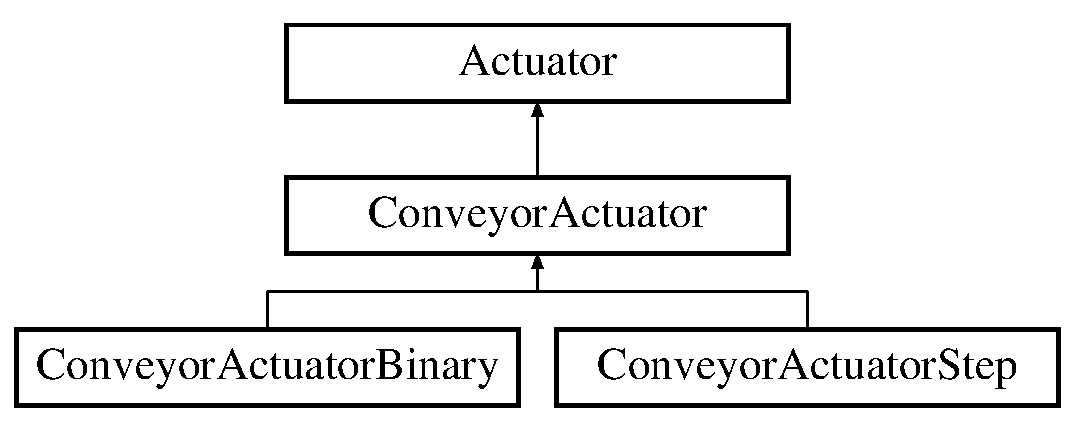
\includegraphics[height=3.000000cm]{classConveyorActuator}
\end{center}
\end{figure}
\subsection*{Public Member Functions}
\begin{DoxyCompactItemize}
\item 
\hyperlink{classConveyorActuator_a264ec9b8887442a47d63ce91a9d017ea}{Conveyor\-Actuator} (int id, \hyperlink{classConveyor}{Conveyor} $\ast$conveyor)
\item 
virtual void \hyperlink{classConveyorActuator_a92b62d5cb761e808337d3b9de910a543}{draw\-Label} ()
\item 
virtual void \hyperlink{classConveyorActuator_a4eeadeec24502aed450880cba04e2784}{set} (signed int value)
\item 
virtual void \hyperlink{classConveyorActuator_a0df274add7b944f869e9486fce8240b1}{run} ()
\end{DoxyCompactItemize}
\subsection*{Public Attributes}
\begin{DoxyCompactItemize}
\item 
\hyperlink{classConveyor}{Conveyor} $\ast$ \hyperlink{classConveyorActuator_a45ff28827d8db7a844b0043383489b7a}{m\-\_\-conveyor}
\end{DoxyCompactItemize}


\subsection{Detailed Description}
Abstact class from which conveyor-\/actuators inherit. 

\subsection{Constructor \& Destructor Documentation}
\hypertarget{classConveyorActuator_a264ec9b8887442a47d63ce91a9d017ea}{\index{Conveyor\-Actuator@{Conveyor\-Actuator}!Conveyor\-Actuator@{Conveyor\-Actuator}}
\index{Conveyor\-Actuator@{Conveyor\-Actuator}!ConveyorActuator@{Conveyor\-Actuator}}
\subsubsection[{Conveyor\-Actuator}]{\setlength{\rightskip}{0pt plus 5cm}Conveyor\-Actuator\-::\-Conveyor\-Actuator (
\begin{DoxyParamCaption}
\item[{int}]{id, }
\item[{{\bf Conveyor} $\ast$}]{conveyor}
\end{DoxyParamCaption}
)}}\label{classConveyorActuator_a264ec9b8887442a47d63ce91a9d017ea}


\subsection{Member Function Documentation}
\hypertarget{classConveyorActuator_a92b62d5cb761e808337d3b9de910a543}{\index{Conveyor\-Actuator@{Conveyor\-Actuator}!draw\-Label@{draw\-Label}}
\index{draw\-Label@{draw\-Label}!ConveyorActuator@{Conveyor\-Actuator}}
\subsubsection[{draw\-Label}]{\setlength{\rightskip}{0pt plus 5cm}void Conveyor\-Actuator\-::draw\-Label (
\begin{DoxyParamCaption}
{}
\end{DoxyParamCaption}
)\hspace{0.3cm}{\ttfamily [virtual]}}}\label{classConveyorActuator_a92b62d5cb761e808337d3b9de910a543}


Reimplemented from \hyperlink{classActuator_aaa39a438315ac34dbb1a4237bf70ff99}{Actuator}.

\hypertarget{classConveyorActuator_a0df274add7b944f869e9486fce8240b1}{\index{Conveyor\-Actuator@{Conveyor\-Actuator}!run@{run}}
\index{run@{run}!ConveyorActuator@{Conveyor\-Actuator}}
\subsubsection[{run}]{\setlength{\rightskip}{0pt plus 5cm}virtual void Conveyor\-Actuator\-::run (
\begin{DoxyParamCaption}
{}
\end{DoxyParamCaption}
)\hspace{0.3cm}{\ttfamily [inline]}, {\ttfamily [virtual]}}}\label{classConveyorActuator_a0df274add7b944f869e9486fce8240b1}


Reimplemented from \hyperlink{classActuator_aabe48a4249a91a4cd1b964001fe754fc}{Actuator}.



Reimplemented in \hyperlink{classConveyorActuatorStep_a07d92edbe704485cadea21988d263201}{Conveyor\-Actuator\-Step}.

\hypertarget{classConveyorActuator_a4eeadeec24502aed450880cba04e2784}{\index{Conveyor\-Actuator@{Conveyor\-Actuator}!set@{set}}
\index{set@{set}!ConveyorActuator@{Conveyor\-Actuator}}
\subsubsection[{set}]{\setlength{\rightskip}{0pt plus 5cm}virtual void Conveyor\-Actuator\-::set (
\begin{DoxyParamCaption}
\item[{signed int}]{value}
\end{DoxyParamCaption}
)\hspace{0.3cm}{\ttfamily [inline]}, {\ttfamily [virtual]}}}\label{classConveyorActuator_a4eeadeec24502aed450880cba04e2784}


Reimplemented from \hyperlink{classActuator_a6281019cccd4034ab2cf7071defecf70}{Actuator}.



Reimplemented in \hyperlink{classConveyorActuatorStep_a7aa64b6b41c86fe4efac32f0090f60f9}{Conveyor\-Actuator\-Step}, and \hyperlink{classConveyorActuatorBinary_a7b546c90b95e289cc0b618001fc934f8}{Conveyor\-Actuator\-Binary}.



\subsection{Member Data Documentation}
\hypertarget{classConveyorActuator_a45ff28827d8db7a844b0043383489b7a}{\index{Conveyor\-Actuator@{Conveyor\-Actuator}!m\-\_\-conveyor@{m\-\_\-conveyor}}
\index{m\-\_\-conveyor@{m\-\_\-conveyor}!ConveyorActuator@{Conveyor\-Actuator}}
\subsubsection[{m\-\_\-conveyor}]{\setlength{\rightskip}{0pt plus 5cm}{\bf Conveyor}$\ast$ Conveyor\-Actuator\-::m\-\_\-conveyor}}\label{classConveyorActuator_a45ff28827d8db7a844b0043383489b7a}


The documentation for this class was generated from the following files\-:\begin{DoxyCompactItemize}
\item 
\hyperlink{Actuators_8h}{Actuators.\-h}\item 
\hyperlink{Actuators_8cpp}{Actuators.\-cpp}\end{DoxyCompactItemize}

\hypertarget{classConveyorActuatorBinary}{\section{Conveyor\-Actuator\-Binary Class Reference}
\label{classConveyorActuatorBinary}\index{Conveyor\-Actuator\-Binary@{Conveyor\-Actuator\-Binary}}
}


Turn a conveyor O\-N or O\-F\-F.  




{\ttfamily \#include $<$Actuators.\-h$>$}

Inheritance diagram for Conveyor\-Actuator\-Binary\-:\begin{figure}[H]
\begin{center}
\leavevmode
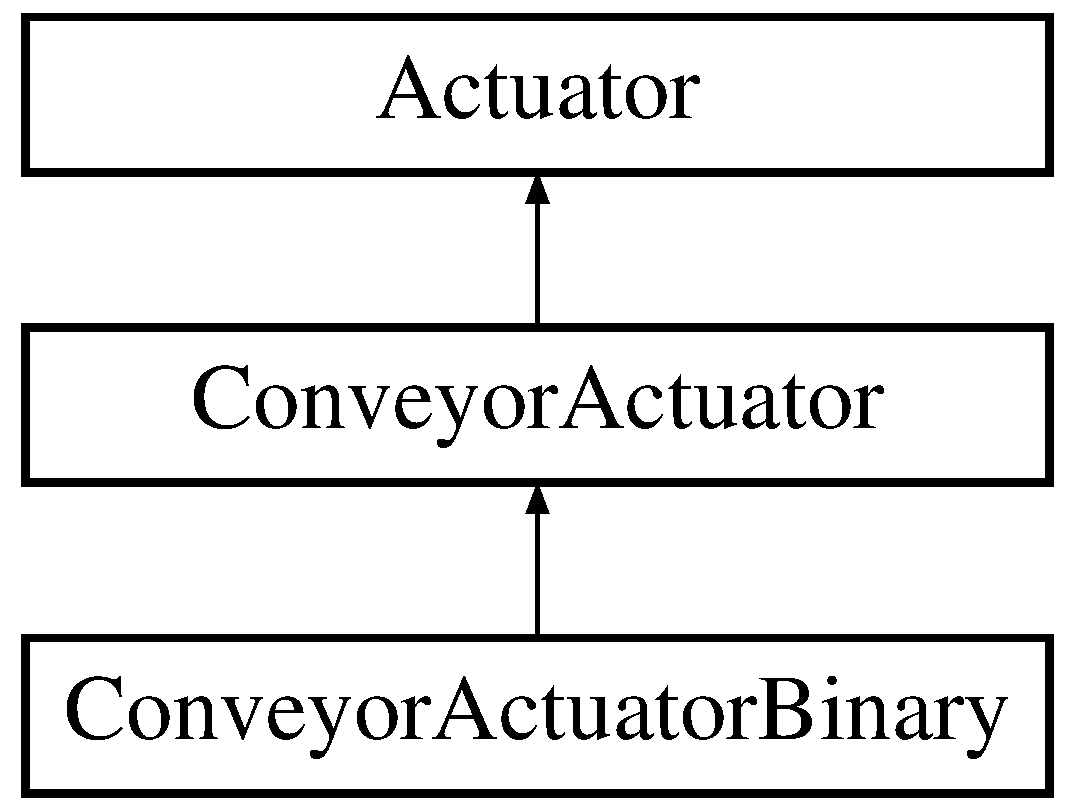
\includegraphics[height=3.000000cm]{classConveyorActuatorBinary}
\end{center}
\end{figure}
\subsection*{Public Member Functions}
\begin{DoxyCompactItemize}
\item 
\hyperlink{classConveyorActuatorBinary_a29bc7ca82221ef79d87c53150b1339e9}{Conveyor\-Actuator\-Binary} (int id, \hyperlink{classConveyor}{Conveyor} $\ast$conveyor)
\item 
void \hyperlink{classConveyorActuatorBinary_a7b546c90b95e289cc0b618001fc934f8}{set} (signed int value)
\end{DoxyCompactItemize}
\subsection*{Additional Inherited Members}


\subsection{Detailed Description}
Turn a conveyor O\-N or O\-F\-F. 

\subsection{Constructor \& Destructor Documentation}
\hypertarget{classConveyorActuatorBinary_a29bc7ca82221ef79d87c53150b1339e9}{\index{Conveyor\-Actuator\-Binary@{Conveyor\-Actuator\-Binary}!Conveyor\-Actuator\-Binary@{Conveyor\-Actuator\-Binary}}
\index{Conveyor\-Actuator\-Binary@{Conveyor\-Actuator\-Binary}!ConveyorActuatorBinary@{Conveyor\-Actuator\-Binary}}
\subsubsection[{Conveyor\-Actuator\-Binary}]{\setlength{\rightskip}{0pt plus 5cm}Conveyor\-Actuator\-Binary\-::\-Conveyor\-Actuator\-Binary (
\begin{DoxyParamCaption}
\item[{int}]{id, }
\item[{{\bf Conveyor} $\ast$}]{conveyor}
\end{DoxyParamCaption}
)}}\label{classConveyorActuatorBinary_a29bc7ca82221ef79d87c53150b1339e9}


\subsection{Member Function Documentation}
\hypertarget{classConveyorActuatorBinary_a7b546c90b95e289cc0b618001fc934f8}{\index{Conveyor\-Actuator\-Binary@{Conveyor\-Actuator\-Binary}!set@{set}}
\index{set@{set}!ConveyorActuatorBinary@{Conveyor\-Actuator\-Binary}}
\subsubsection[{set}]{\setlength{\rightskip}{0pt plus 5cm}void Conveyor\-Actuator\-Binary\-::set (
\begin{DoxyParamCaption}
\item[{signed int}]{value}
\end{DoxyParamCaption}
)\hspace{0.3cm}{\ttfamily [virtual]}}}\label{classConveyorActuatorBinary_a7b546c90b95e289cc0b618001fc934f8}


Reimplemented from \hyperlink{classConveyorActuator_a4eeadeec24502aed450880cba04e2784}{Conveyor\-Actuator}.



The documentation for this class was generated from the following files\-:\begin{DoxyCompactItemize}
\item 
\hyperlink{Actuators_8h}{Actuators.\-h}\item 
\hyperlink{Actuators_8cpp}{Actuators.\-cpp}\end{DoxyCompactItemize}

\hypertarget{classConveyorActuatorStep}{\section{Conveyor\-Actuator\-Step Class Reference}
\label{classConveyorActuatorStep}\index{Conveyor\-Actuator\-Step@{Conveyor\-Actuator\-Step}}
}


Run a conveyor an arbitrary number of steps.  




{\ttfamily \#include $<$Actuators.\-h$>$}

Inheritance diagram for Conveyor\-Actuator\-Step\-:\begin{figure}[H]
\begin{center}
\leavevmode
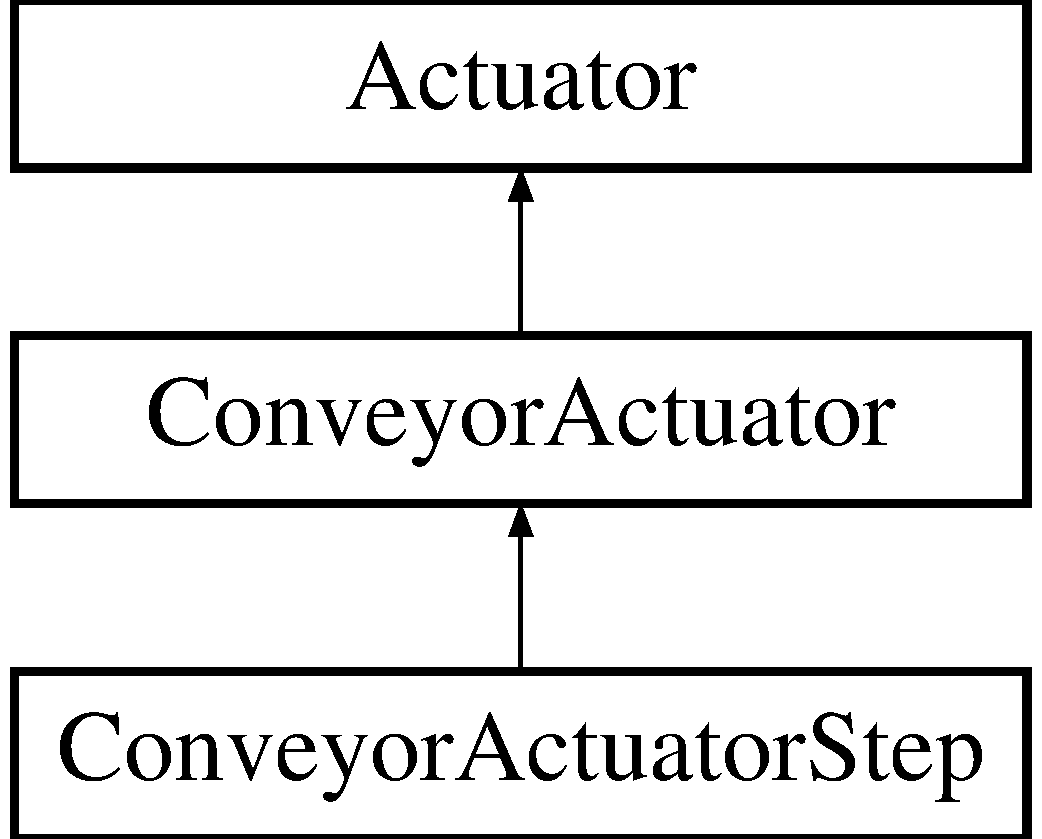
\includegraphics[height=3.000000cm]{classConveyorActuatorStep}
\end{center}
\end{figure}
\subsection*{Public Member Functions}
\begin{DoxyCompactItemize}
\item 
\hyperlink{classConveyorActuatorStep_adfdfa7103dff9ca883cfb268746fbf88}{Conveyor\-Actuator\-Step} (int id, \hyperlink{classConveyor}{Conveyor} $\ast$conveyor)
\item 
void \hyperlink{classConveyorActuatorStep_a7aa64b6b41c86fe4efac32f0090f60f9}{set} (signed int value)
\item 
void \hyperlink{classConveyorActuatorStep_a07d92edbe704485cadea21988d263201}{run} ()
\end{DoxyCompactItemize}
\subsection*{Public Attributes}
\begin{DoxyCompactItemize}
\item 
float32 \hyperlink{classConveyorActuatorStep_abb724c62bd72162123dff985ae961ce1}{m\-\_\-start\-Angle}
\item 
float32 \hyperlink{classConveyorActuatorStep_abe8e93d72ff0637b80583cb8c4a7ea24}{m\-\_\-max\-Rotation}
\end{DoxyCompactItemize}


\subsection{Detailed Description}
Run a conveyor an arbitrary number of steps. 

\subsection{Constructor \& Destructor Documentation}
\hypertarget{classConveyorActuatorStep_adfdfa7103dff9ca883cfb268746fbf88}{\index{Conveyor\-Actuator\-Step@{Conveyor\-Actuator\-Step}!Conveyor\-Actuator\-Step@{Conveyor\-Actuator\-Step}}
\index{Conveyor\-Actuator\-Step@{Conveyor\-Actuator\-Step}!ConveyorActuatorStep@{Conveyor\-Actuator\-Step}}
\subsubsection[{Conveyor\-Actuator\-Step}]{\setlength{\rightskip}{0pt plus 5cm}Conveyor\-Actuator\-Step\-::\-Conveyor\-Actuator\-Step (
\begin{DoxyParamCaption}
\item[{int}]{id, }
\item[{{\bf Conveyor} $\ast$}]{conveyor}
\end{DoxyParamCaption}
)}}\label{classConveyorActuatorStep_adfdfa7103dff9ca883cfb268746fbf88}


\subsection{Member Function Documentation}
\hypertarget{classConveyorActuatorStep_a07d92edbe704485cadea21988d263201}{\index{Conveyor\-Actuator\-Step@{Conveyor\-Actuator\-Step}!run@{run}}
\index{run@{run}!ConveyorActuatorStep@{Conveyor\-Actuator\-Step}}
\subsubsection[{run}]{\setlength{\rightskip}{0pt plus 5cm}void Conveyor\-Actuator\-Step\-::run (
\begin{DoxyParamCaption}
{}
\end{DoxyParamCaption}
)\hspace{0.3cm}{\ttfamily [virtual]}}}\label{classConveyorActuatorStep_a07d92edbe704485cadea21988d263201}


Reimplemented from \hyperlink{classConveyorActuator_a0df274add7b944f869e9486fce8240b1}{Conveyor\-Actuator}.

\hypertarget{classConveyorActuatorStep_a7aa64b6b41c86fe4efac32f0090f60f9}{\index{Conveyor\-Actuator\-Step@{Conveyor\-Actuator\-Step}!set@{set}}
\index{set@{set}!ConveyorActuatorStep@{Conveyor\-Actuator\-Step}}
\subsubsection[{set}]{\setlength{\rightskip}{0pt plus 5cm}void Conveyor\-Actuator\-Step\-::set (
\begin{DoxyParamCaption}
\item[{signed int}]{value}
\end{DoxyParamCaption}
)\hspace{0.3cm}{\ttfamily [virtual]}}}\label{classConveyorActuatorStep_a7aa64b6b41c86fe4efac32f0090f60f9}


Reimplemented from \hyperlink{classConveyorActuator_a4eeadeec24502aed450880cba04e2784}{Conveyor\-Actuator}.



\subsection{Member Data Documentation}
\hypertarget{classConveyorActuatorStep_abe8e93d72ff0637b80583cb8c4a7ea24}{\index{Conveyor\-Actuator\-Step@{Conveyor\-Actuator\-Step}!m\-\_\-max\-Rotation@{m\-\_\-max\-Rotation}}
\index{m\-\_\-max\-Rotation@{m\-\_\-max\-Rotation}!ConveyorActuatorStep@{Conveyor\-Actuator\-Step}}
\subsubsection[{m\-\_\-max\-Rotation}]{\setlength{\rightskip}{0pt plus 5cm}float32 Conveyor\-Actuator\-Step\-::m\-\_\-max\-Rotation}}\label{classConveyorActuatorStep_abe8e93d72ff0637b80583cb8c4a7ea24}
\hypertarget{classConveyorActuatorStep_abb724c62bd72162123dff985ae961ce1}{\index{Conveyor\-Actuator\-Step@{Conveyor\-Actuator\-Step}!m\-\_\-start\-Angle@{m\-\_\-start\-Angle}}
\index{m\-\_\-start\-Angle@{m\-\_\-start\-Angle}!ConveyorActuatorStep@{Conveyor\-Actuator\-Step}}
\subsubsection[{m\-\_\-start\-Angle}]{\setlength{\rightskip}{0pt plus 5cm}float32 Conveyor\-Actuator\-Step\-::m\-\_\-start\-Angle}}\label{classConveyorActuatorStep_abb724c62bd72162123dff985ae961ce1}


The documentation for this class was generated from the following files\-:\begin{DoxyCompactItemize}
\item 
\hyperlink{Actuators_8h}{Actuators.\-h}\item 
\hyperlink{Actuators_8cpp}{Actuators.\-cpp}\end{DoxyCompactItemize}

\hypertarget{classConveyorBelt}{\section{Conveyor\-Belt Class Reference}
\label{classConveyorBelt}\index{Conveyor\-Belt@{Conveyor\-Belt}}
}


The conveyorbelt.  




{\ttfamily \#include $<$Conveyor.\-h$>$}

\subsection*{Public Member Functions}
\begin{DoxyCompactItemize}
\item 
\hyperlink{classConveyorBelt_a054992c219cd54cffd1b31aa819c25f0}{Conveyor\-Belt} (b2\-Vec2 p1, b2\-Vec2 p2, float32 beam\-Thickness, float32 belt\-Thickness, int N, int M, \hyperlink{Conveyor_8h_a98261db3679be2885c0bdad13c27d7b1}{t\-\_\-medbringer\-Type} medbringer\-Type, int sensor\-Pos, float32 sensor\-Adjustment, int cm\-Bits, b2\-World $\ast$world)
\begin{DoxyCompactList}\small\item\em Create the conveyorbelt. \end{DoxyCompactList}\item 
float32 \hyperlink{classConveyorBelt_acf80525e6c5e618ffac5c8e8d0eed38c}{get\-Angle\-At} (b2\-Vec2 p)
\item 
void \hyperlink{classConveyorBelt_accae6e53d7d8e37e86aa9d4649c64481}{pause} ()
\item 
void \hyperlink{classConveyorBelt_af862468684b4bf0f1b05141ea8ee7943}{play} ()
\item 
\hyperlink{classContactSensor}{Contact\-Sensor} $\ast$ \hyperlink{classConveyorBelt_ada62b4755b222ef7a07233d5478c67a2}{get\-Sensor} ()
\end{DoxyCompactItemize}
\subsection*{Public Attributes}
\begin{DoxyCompactItemize}
\item 
b2\-Vec2 \hyperlink{classConveyorBelt_ad22553d91da070067703878c4059ecf5}{m\-\_\-p1}
\item 
b2\-Vec2 \hyperlink{classConveyorBelt_a061584c0f9fe736cd06d5b81472016dd}{m\-\_\-p2}
\item 
vector$<$ b2\-Body $\ast$ $>$ \hyperlink{classConveyorBelt_a21237fddbc2791faf8e26fd346ac8434}{link}
\item 
vector$<$ b2\-Vec2 $>$ \hyperlink{classConveyorBelt_a1dbc93fa0310c47d89f234602fc8610e}{link\-Speed}
\item 
bool \hyperlink{classConveyorBelt_a2325f44e6279a81a6927020e97f725a3}{m\-\_\-paused}
\item 
\hyperlink{classContactSensor__Sync}{Contact\-Sensor\-\_\-\-Sync} $\ast$ \hyperlink{classConveyorBelt_a35e3eacb4d9a46fd58505dba22a020c5}{m\-\_\-contact\-Sensor\-Circular}
\item 
\hyperlink{Conveyor_8h_a98261db3679be2885c0bdad13c27d7b1}{t\-\_\-medbringer\-Type} \hyperlink{classConveyorBelt_a92464da95aad2012ab4fcb0c1a998f42}{m\-\_\-medbringer\-Type}
\end{DoxyCompactItemize}


\subsection{Detailed Description}
The conveyorbelt. 

\subsection{Constructor \& Destructor Documentation}
\hypertarget{classConveyorBelt_a054992c219cd54cffd1b31aa819c25f0}{\index{Conveyor\-Belt@{Conveyor\-Belt}!Conveyor\-Belt@{Conveyor\-Belt}}
\index{Conveyor\-Belt@{Conveyor\-Belt}!ConveyorBelt@{Conveyor\-Belt}}
\subsubsection[{Conveyor\-Belt}]{\setlength{\rightskip}{0pt plus 5cm}Conveyor\-Belt\-::\-Conveyor\-Belt (
\begin{DoxyParamCaption}
\item[{b2\-Vec2}]{p1, }
\item[{b2\-Vec2}]{p2, }
\item[{float32}]{beam\-Thickness, }
\item[{float32}]{belt\-Thickness, }
\item[{int}]{N, }
\item[{int}]{M, }
\item[{{\bf t\-\_\-medbringer\-Type}}]{medbringer\-Type, }
\item[{int}]{sensor\-Pos, }
\item[{float32}]{sensor\-Adjustment, }
\item[{int}]{cm\-Bits, }
\item[{b2\-World $\ast$}]{world}
\end{DoxyParamCaption}
)}}\label{classConveyorBelt_a054992c219cd54cffd1b31aa819c25f0}


Create the conveyorbelt. 


\begin{DoxyParams}{Parameters}
{\em p1} & Center position of first wheel. \\
\hline
{\em p2} & Center position of second wheel. \\
\hline
{\em beam\-Thickness} & Thickness of the beam. \\
\hline
{\em belt\-Thickness} & Thickness of the belt. \\
\hline
{\em N} & Number of links. \\
\hline
{\em M} & Number of links between every \char`\"{}medbringer\char`\"{} \\
\hline
{\em medbringer\-Type} & The type of \char`\"{}medbringers\char`\"{} which are connected to the belt. \\
\hline
{\em sensor\-Pos} & The number of the link which the sensor is placed at. \\
\hline
{\em sensor\-Adjustment} & \\
\hline
{\em cm\-Bits} & Category-\/ and mask-\/bits. \\
\hline
{\em world} & Pointer to the world in which you want to create a conveyorbelt. \\
\hline
\end{DoxyParams}


\subsection{Member Function Documentation}
\hypertarget{classConveyorBelt_acf80525e6c5e618ffac5c8e8d0eed38c}{\index{Conveyor\-Belt@{Conveyor\-Belt}!get\-Angle\-At@{get\-Angle\-At}}
\index{get\-Angle\-At@{get\-Angle\-At}!ConveyorBelt@{Conveyor\-Belt}}
\subsubsection[{get\-Angle\-At}]{\setlength{\rightskip}{0pt plus 5cm}float32 Conveyor\-Belt\-::get\-Angle\-At (
\begin{DoxyParamCaption}
\item[{b2\-Vec2}]{p}
\end{DoxyParamCaption}
)}}\label{classConveyorBelt_acf80525e6c5e618ffac5c8e8d0eed38c}
Get the angle of the nearest belt-\/tangent \hypertarget{classConveyorBelt_ada62b4755b222ef7a07233d5478c67a2}{\index{Conveyor\-Belt@{Conveyor\-Belt}!get\-Sensor@{get\-Sensor}}
\index{get\-Sensor@{get\-Sensor}!ConveyorBelt@{Conveyor\-Belt}}
\subsubsection[{get\-Sensor}]{\setlength{\rightskip}{0pt plus 5cm}{\bf Contact\-Sensor}$\ast$ Conveyor\-Belt\-::get\-Sensor (
\begin{DoxyParamCaption}
{}
\end{DoxyParamCaption}
)\hspace{0.3cm}{\ttfamily [inline]}}}\label{classConveyorBelt_ada62b4755b222ef7a07233d5478c67a2}
Return the synchronization sensor \hypertarget{classConveyorBelt_accae6e53d7d8e37e86aa9d4649c64481}{\index{Conveyor\-Belt@{Conveyor\-Belt}!pause@{pause}}
\index{pause@{pause}!ConveyorBelt@{Conveyor\-Belt}}
\subsubsection[{pause}]{\setlength{\rightskip}{0pt plus 5cm}void Conveyor\-Belt\-::pause (
\begin{DoxyParamCaption}
{}
\end{DoxyParamCaption}
)}}\label{classConveyorBelt_accae6e53d7d8e37e86aa9d4649c64481}
Pause the belt \hypertarget{classConveyorBelt_af862468684b4bf0f1b05141ea8ee7943}{\index{Conveyor\-Belt@{Conveyor\-Belt}!play@{play}}
\index{play@{play}!ConveyorBelt@{Conveyor\-Belt}}
\subsubsection[{play}]{\setlength{\rightskip}{0pt plus 5cm}void Conveyor\-Belt\-::play (
\begin{DoxyParamCaption}
{}
\end{DoxyParamCaption}
)}}\label{classConveyorBelt_af862468684b4bf0f1b05141ea8ee7943}
Restart the belt in the same state as when paused. 

\subsection{Member Data Documentation}
\hypertarget{classConveyorBelt_a21237fddbc2791faf8e26fd346ac8434}{\index{Conveyor\-Belt@{Conveyor\-Belt}!link@{link}}
\index{link@{link}!ConveyorBelt@{Conveyor\-Belt}}
\subsubsection[{link}]{\setlength{\rightskip}{0pt plus 5cm}vector$<$b2\-Body$\ast$$>$ Conveyor\-Belt\-::link}}\label{classConveyorBelt_a21237fddbc2791faf8e26fd346ac8434}
\hypertarget{classConveyorBelt_a1dbc93fa0310c47d89f234602fc8610e}{\index{Conveyor\-Belt@{Conveyor\-Belt}!link\-Speed@{link\-Speed}}
\index{link\-Speed@{link\-Speed}!ConveyorBelt@{Conveyor\-Belt}}
\subsubsection[{link\-Speed}]{\setlength{\rightskip}{0pt plus 5cm}vector$<$b2\-Vec2$>$ Conveyor\-Belt\-::link\-Speed}}\label{classConveyorBelt_a1dbc93fa0310c47d89f234602fc8610e}
List of all the links velocity-\/ vectors \hypertarget{classConveyorBelt_a35e3eacb4d9a46fd58505dba22a020c5}{\index{Conveyor\-Belt@{Conveyor\-Belt}!m\-\_\-contact\-Sensor\-Circular@{m\-\_\-contact\-Sensor\-Circular}}
\index{m\-\_\-contact\-Sensor\-Circular@{m\-\_\-contact\-Sensor\-Circular}!ConveyorBelt@{Conveyor\-Belt}}
\subsubsection[{m\-\_\-contact\-Sensor\-Circular}]{\setlength{\rightskip}{0pt plus 5cm}{\bf Contact\-Sensor\-\_\-\-Sync}$\ast$ Conveyor\-Belt\-::m\-\_\-contact\-Sensor\-Circular}}\label{classConveyorBelt_a35e3eacb4d9a46fd58505dba22a020c5}
\hypertarget{classConveyorBelt_a92464da95aad2012ab4fcb0c1a998f42}{\index{Conveyor\-Belt@{Conveyor\-Belt}!m\-\_\-medbringer\-Type@{m\-\_\-medbringer\-Type}}
\index{m\-\_\-medbringer\-Type@{m\-\_\-medbringer\-Type}!ConveyorBelt@{Conveyor\-Belt}}
\subsubsection[{m\-\_\-medbringer\-Type}]{\setlength{\rightskip}{0pt plus 5cm}{\bf t\-\_\-medbringer\-Type} Conveyor\-Belt\-::m\-\_\-medbringer\-Type}}\label{classConveyorBelt_a92464da95aad2012ab4fcb0c1a998f42}
\hypertarget{classConveyorBelt_ad22553d91da070067703878c4059ecf5}{\index{Conveyor\-Belt@{Conveyor\-Belt}!m\-\_\-p1@{m\-\_\-p1}}
\index{m\-\_\-p1@{m\-\_\-p1}!ConveyorBelt@{Conveyor\-Belt}}
\subsubsection[{m\-\_\-p1}]{\setlength{\rightskip}{0pt plus 5cm}b2\-Vec2 Conveyor\-Belt\-::m\-\_\-p1}}\label{classConveyorBelt_ad22553d91da070067703878c4059ecf5}
\hypertarget{classConveyorBelt_a061584c0f9fe736cd06d5b81472016dd}{\index{Conveyor\-Belt@{Conveyor\-Belt}!m\-\_\-p2@{m\-\_\-p2}}
\index{m\-\_\-p2@{m\-\_\-p2}!ConveyorBelt@{Conveyor\-Belt}}
\subsubsection[{m\-\_\-p2}]{\setlength{\rightskip}{0pt plus 5cm}b2\-Vec2 Conveyor\-Belt\-::m\-\_\-p2}}\label{classConveyorBelt_a061584c0f9fe736cd06d5b81472016dd}
\hypertarget{classConveyorBelt_a2325f44e6279a81a6927020e97f725a3}{\index{Conveyor\-Belt@{Conveyor\-Belt}!m\-\_\-paused@{m\-\_\-paused}}
\index{m\-\_\-paused@{m\-\_\-paused}!ConveyorBelt@{Conveyor\-Belt}}
\subsubsection[{m\-\_\-paused}]{\setlength{\rightskip}{0pt plus 5cm}bool Conveyor\-Belt\-::m\-\_\-paused}}\label{classConveyorBelt_a2325f44e6279a81a6927020e97f725a3}


The documentation for this class was generated from the following files\-:\begin{DoxyCompactItemize}
\item 
\hyperlink{Conveyor_8h}{Conveyor.\-h}\item 
\hyperlink{Conveyor_8cpp}{Conveyor.\-cpp}\end{DoxyCompactItemize}

\hypertarget{classConveyorBeltShield}{\section{Conveyor\-Belt\-Shield Class Reference}
\label{classConveyorBeltShield}\index{Conveyor\-Belt\-Shield@{Conveyor\-Belt\-Shield}}
}


Hinder the conveyorbelt in falling off.  




{\ttfamily \#include $<$Conveyor.\-h$>$}

\subsection*{Public Member Functions}
\begin{DoxyCompactItemize}
\item 
\hyperlink{classConveyorBeltShield_a814f92c11fe70adfc3b6f033357ebf3a}{Conveyor\-Belt\-Shield} (b2\-Vec2 p1, b2\-Vec2 p2, float32 beam\-Thickness, float32 belt\-Thickness, int cm\-Bits, b2\-World $\ast$world)
\end{DoxyCompactItemize}
\subsection*{Public Attributes}
\begin{DoxyCompactItemize}
\item 
b2\-Vec2 \hyperlink{classConveyorBeltShield_a28e34cf663b048519e8af9412b42c638}{m\-\_\-p1}
\item 
b2\-Vec2 \hyperlink{classConveyorBeltShield_a2bc6d812e1e50d7be3f7ddb97b29f0dd}{m\-\_\-p2}
\item 
float32 \hyperlink{classConveyorBeltShield_a026153ef70d96c0e835861467cc1a02c}{m\-\_\-beam\-Thickness}
\item 
float32 \hyperlink{classConveyorBeltShield_a793a55bd4b34b9e2a6c89b457373f01d}{m\-\_\-belt\-Thickness}
\end{DoxyCompactItemize}


\subsection{Detailed Description}
Hinder the conveyorbelt in falling off. 

\subsection{Constructor \& Destructor Documentation}
\hypertarget{classConveyorBeltShield_a814f92c11fe70adfc3b6f033357ebf3a}{\index{Conveyor\-Belt\-Shield@{Conveyor\-Belt\-Shield}!Conveyor\-Belt\-Shield@{Conveyor\-Belt\-Shield}}
\index{Conveyor\-Belt\-Shield@{Conveyor\-Belt\-Shield}!ConveyorBeltShield@{Conveyor\-Belt\-Shield}}
\subsubsection[{Conveyor\-Belt\-Shield}]{\setlength{\rightskip}{0pt plus 5cm}Conveyor\-Belt\-Shield\-::\-Conveyor\-Belt\-Shield (
\begin{DoxyParamCaption}
\item[{b2\-Vec2}]{p1, }
\item[{b2\-Vec2}]{p2, }
\item[{float32}]{beam\-Thickness, }
\item[{float32}]{belt\-Thickness, }
\item[{int}]{cm\-Bits, }
\item[{b2\-World $\ast$}]{world}
\end{DoxyParamCaption}
)}}\label{classConveyorBeltShield_a814f92c11fe70adfc3b6f033357ebf3a}


\subsection{Member Data Documentation}
\hypertarget{classConveyorBeltShield_a026153ef70d96c0e835861467cc1a02c}{\index{Conveyor\-Belt\-Shield@{Conveyor\-Belt\-Shield}!m\-\_\-beam\-Thickness@{m\-\_\-beam\-Thickness}}
\index{m\-\_\-beam\-Thickness@{m\-\_\-beam\-Thickness}!ConveyorBeltShield@{Conveyor\-Belt\-Shield}}
\subsubsection[{m\-\_\-beam\-Thickness}]{\setlength{\rightskip}{0pt plus 5cm}float32 Conveyor\-Belt\-Shield\-::m\-\_\-beam\-Thickness}}\label{classConveyorBeltShield_a026153ef70d96c0e835861467cc1a02c}
\hypertarget{classConveyorBeltShield_a793a55bd4b34b9e2a6c89b457373f01d}{\index{Conveyor\-Belt\-Shield@{Conveyor\-Belt\-Shield}!m\-\_\-belt\-Thickness@{m\-\_\-belt\-Thickness}}
\index{m\-\_\-belt\-Thickness@{m\-\_\-belt\-Thickness}!ConveyorBeltShield@{Conveyor\-Belt\-Shield}}
\subsubsection[{m\-\_\-belt\-Thickness}]{\setlength{\rightskip}{0pt plus 5cm}float32 Conveyor\-Belt\-Shield\-::m\-\_\-belt\-Thickness}}\label{classConveyorBeltShield_a793a55bd4b34b9e2a6c89b457373f01d}
\hypertarget{classConveyorBeltShield_a28e34cf663b048519e8af9412b42c638}{\index{Conveyor\-Belt\-Shield@{Conveyor\-Belt\-Shield}!m\-\_\-p1@{m\-\_\-p1}}
\index{m\-\_\-p1@{m\-\_\-p1}!ConveyorBeltShield@{Conveyor\-Belt\-Shield}}
\subsubsection[{m\-\_\-p1}]{\setlength{\rightskip}{0pt plus 5cm}b2\-Vec2 Conveyor\-Belt\-Shield\-::m\-\_\-p1}}\label{classConveyorBeltShield_a28e34cf663b048519e8af9412b42c638}
\hypertarget{classConveyorBeltShield_a2bc6d812e1e50d7be3f7ddb97b29f0dd}{\index{Conveyor\-Belt\-Shield@{Conveyor\-Belt\-Shield}!m\-\_\-p2@{m\-\_\-p2}}
\index{m\-\_\-p2@{m\-\_\-p2}!ConveyorBeltShield@{Conveyor\-Belt\-Shield}}
\subsubsection[{m\-\_\-p2}]{\setlength{\rightskip}{0pt plus 5cm}b2\-Vec2 Conveyor\-Belt\-Shield\-::m\-\_\-p2}}\label{classConveyorBeltShield_a2bc6d812e1e50d7be3f7ddb97b29f0dd}


The documentation for this class was generated from the following files\-:\begin{DoxyCompactItemize}
\item 
\hyperlink{Conveyor_8h}{Conveyor.\-h}\item 
\hyperlink{Conveyor_8cpp}{Conveyor.\-cpp}\end{DoxyCompactItemize}

\hypertarget{classConveyorSynchronizer}{\section{Conveyor\-Synchronizer Class Reference}
\label{classConveyorSynchronizer}\index{Conveyor\-Synchronizer@{Conveyor\-Synchronizer}}
}


Synchronize Conveyors.  




{\ttfamily \#include $<$Conveyor\-Synchronizer.\-h$>$}

\subsection*{Public Types}
\begin{DoxyCompactItemize}
\item 
enum \hyperlink{classConveyorSynchronizer_ad503ce87e58a6567d30daf11bf9b97b5}{states\-\_\-type} \{ \hyperlink{classConveyorSynchronizer_ad503ce87e58a6567d30daf11bf9b97b5ae6a6f6526745c204c0b2be970d0522a2}{st1}, 
\hyperlink{classConveyorSynchronizer_ad503ce87e58a6567d30daf11bf9b97b5a6c75db9fef7dbca83dc368a261065f1a}{st2}
 \}
\end{DoxyCompactItemize}
\subsection*{Public Member Functions}
\begin{DoxyCompactItemize}
\item 
\hyperlink{classConveyorSynchronizer_ae197fb7a2b8b53ec8425e736ed26d508}{Conveyor\-Synchronizer} ()
\item 
void \hyperlink{classConveyorSynchronizer_ae640bf1ee6bbf1f61f2a9430df93fe06}{add} (\hyperlink{classConveyor}{Conveyor} $\ast$conveyor)
\begin{DoxyCompactList}\small\item\em Add as many conveyers as you'd like. \end{DoxyCompactList}\item 
void \hyperlink{classConveyorSynchronizer_ae30b7c917a6522f4ae17d747b9f88ee0}{run} ()
\begin{DoxyCompactList}\small\item\em Place this function in a loop to run the synchronization. \end{DoxyCompactList}\end{DoxyCompactItemize}
\subsection*{Public Attributes}
\begin{DoxyCompactItemize}
\item 
\hyperlink{classConveyor}{Conveyor} $\ast$ \hyperlink{classConveyorSynchronizer_a0b3932b4b2eb980377a01913ac7e31f7}{m\-\_\-conveyor1}
\item 
\hyperlink{classConveyor}{Conveyor} $\ast$ \hyperlink{classConveyorSynchronizer_a6d409ca27bf95110c977946158da2fed}{m\-\_\-conveyor2}
\item 
\hyperlink{classConveyorSynchronizer_ad503ce87e58a6567d30daf11bf9b97b5}{states\-\_\-type} \hyperlink{classConveyorSynchronizer_a74ead75da9c1863838b34cd288cae02f}{m\-\_\-state}
\item 
bool \hyperlink{classConveyorSynchronizer_aff3ac2926f3771d47d4954cc384e21f3}{initialized}
\item 
vector$<$ \hyperlink{classConveyor}{Conveyor} $\ast$ $>$ \hyperlink{classConveyorSynchronizer_a2df84a539b1399075936bafcb23a874d}{m\-\_\-conveyor}
\item 
int \hyperlink{classConveyorSynchronizer_a9e4513793155c94c434ab6403c937085}{m\-\_\-number\-Of\-Conveyors}
\end{DoxyCompactItemize}


\subsection{Detailed Description}
Synchronize Conveyors. 

\subsection{Member Enumeration Documentation}
\hypertarget{classConveyorSynchronizer_ad503ce87e58a6567d30daf11bf9b97b5}{\index{Conveyor\-Synchronizer@{Conveyor\-Synchronizer}!states\-\_\-type@{states\-\_\-type}}
\index{states\-\_\-type@{states\-\_\-type}!ConveyorSynchronizer@{Conveyor\-Synchronizer}}
\subsubsection[{states\-\_\-type}]{\setlength{\rightskip}{0pt plus 5cm}enum {\bf Conveyor\-Synchronizer\-::states\-\_\-type}}}\label{classConveyorSynchronizer_ad503ce87e58a6567d30daf11bf9b97b5}
\begin{Desc}
\item[Enumerator\-: ]\par
\begin{description}
\index{st1@{st1}!Conveyor\-Synchronizer@{Conveyor\-Synchronizer}}\index{Conveyor\-Synchronizer@{Conveyor\-Synchronizer}!st1@{st1}}\item[{\em 
\hypertarget{classConveyorSynchronizer_ad503ce87e58a6567d30daf11bf9b97b5ae6a6f6526745c204c0b2be970d0522a2}{st1}\label{classConveyorSynchronizer_ad503ce87e58a6567d30daf11bf9b97b5ae6a6f6526745c204c0b2be970d0522a2}
}]\index{st2@{st2}!Conveyor\-Synchronizer@{Conveyor\-Synchronizer}}\index{Conveyor\-Synchronizer@{Conveyor\-Synchronizer}!st2@{st2}}\item[{\em 
\hypertarget{classConveyorSynchronizer_ad503ce87e58a6567d30daf11bf9b97b5a6c75db9fef7dbca83dc368a261065f1a}{st2}\label{classConveyorSynchronizer_ad503ce87e58a6567d30daf11bf9b97b5a6c75db9fef7dbca83dc368a261065f1a}
}]\end{description}
\end{Desc}



\subsection{Constructor \& Destructor Documentation}
\hypertarget{classConveyorSynchronizer_ae197fb7a2b8b53ec8425e736ed26d508}{\index{Conveyor\-Synchronizer@{Conveyor\-Synchronizer}!Conveyor\-Synchronizer@{Conveyor\-Synchronizer}}
\index{Conveyor\-Synchronizer@{Conveyor\-Synchronizer}!ConveyorSynchronizer@{Conveyor\-Synchronizer}}
\subsubsection[{Conveyor\-Synchronizer}]{\setlength{\rightskip}{0pt plus 5cm}Conveyor\-Synchronizer\-::\-Conveyor\-Synchronizer (
\begin{DoxyParamCaption}
{}
\end{DoxyParamCaption}
)}}\label{classConveyorSynchronizer_ae197fb7a2b8b53ec8425e736ed26d508}


\subsection{Member Function Documentation}
\hypertarget{classConveyorSynchronizer_ae640bf1ee6bbf1f61f2a9430df93fe06}{\index{Conveyor\-Synchronizer@{Conveyor\-Synchronizer}!add@{add}}
\index{add@{add}!ConveyorSynchronizer@{Conveyor\-Synchronizer}}
\subsubsection[{add}]{\setlength{\rightskip}{0pt plus 5cm}void Conveyor\-Synchronizer\-::add (
\begin{DoxyParamCaption}
\item[{{\bf Conveyor} $\ast$}]{conveyor}
\end{DoxyParamCaption}
)}}\label{classConveyorSynchronizer_ae640bf1ee6bbf1f61f2a9430df93fe06}


Add as many conveyers as you'd like. 

\hypertarget{classConveyorSynchronizer_ae30b7c917a6522f4ae17d747b9f88ee0}{\index{Conveyor\-Synchronizer@{Conveyor\-Synchronizer}!run@{run}}
\index{run@{run}!ConveyorSynchronizer@{Conveyor\-Synchronizer}}
\subsubsection[{run}]{\setlength{\rightskip}{0pt plus 5cm}void Conveyor\-Synchronizer\-::run (
\begin{DoxyParamCaption}
{}
\end{DoxyParamCaption}
)}}\label{classConveyorSynchronizer_ae30b7c917a6522f4ae17d747b9f88ee0}


Place this function in a loop to run the synchronization. 

(E.\-g in the \hyperlink{classSimulatorPage}{Simulator\-Page} Step(...)-\/block) 

\subsection{Member Data Documentation}
\hypertarget{classConveyorSynchronizer_aff3ac2926f3771d47d4954cc384e21f3}{\index{Conveyor\-Synchronizer@{Conveyor\-Synchronizer}!initialized@{initialized}}
\index{initialized@{initialized}!ConveyorSynchronizer@{Conveyor\-Synchronizer}}
\subsubsection[{initialized}]{\setlength{\rightskip}{0pt plus 5cm}bool Conveyor\-Synchronizer\-::initialized}}\label{classConveyorSynchronizer_aff3ac2926f3771d47d4954cc384e21f3}
\hypertarget{classConveyorSynchronizer_a2df84a539b1399075936bafcb23a874d}{\index{Conveyor\-Synchronizer@{Conveyor\-Synchronizer}!m\-\_\-conveyor@{m\-\_\-conveyor}}
\index{m\-\_\-conveyor@{m\-\_\-conveyor}!ConveyorSynchronizer@{Conveyor\-Synchronizer}}
\subsubsection[{m\-\_\-conveyor}]{\setlength{\rightskip}{0pt plus 5cm}vector$<${\bf Conveyor}$\ast$$>$ Conveyor\-Synchronizer\-::m\-\_\-conveyor}}\label{classConveyorSynchronizer_a2df84a539b1399075936bafcb23a874d}
\hypertarget{classConveyorSynchronizer_a0b3932b4b2eb980377a01913ac7e31f7}{\index{Conveyor\-Synchronizer@{Conveyor\-Synchronizer}!m\-\_\-conveyor1@{m\-\_\-conveyor1}}
\index{m\-\_\-conveyor1@{m\-\_\-conveyor1}!ConveyorSynchronizer@{Conveyor\-Synchronizer}}
\subsubsection[{m\-\_\-conveyor1}]{\setlength{\rightskip}{0pt plus 5cm}{\bf Conveyor}$\ast$ Conveyor\-Synchronizer\-::m\-\_\-conveyor1}}\label{classConveyorSynchronizer_a0b3932b4b2eb980377a01913ac7e31f7}
\hypertarget{classConveyorSynchronizer_a6d409ca27bf95110c977946158da2fed}{\index{Conveyor\-Synchronizer@{Conveyor\-Synchronizer}!m\-\_\-conveyor2@{m\-\_\-conveyor2}}
\index{m\-\_\-conveyor2@{m\-\_\-conveyor2}!ConveyorSynchronizer@{Conveyor\-Synchronizer}}
\subsubsection[{m\-\_\-conveyor2}]{\setlength{\rightskip}{0pt plus 5cm}{\bf Conveyor}$\ast$ Conveyor\-Synchronizer\-::m\-\_\-conveyor2}}\label{classConveyorSynchronizer_a6d409ca27bf95110c977946158da2fed}
\hypertarget{classConveyorSynchronizer_a9e4513793155c94c434ab6403c937085}{\index{Conveyor\-Synchronizer@{Conveyor\-Synchronizer}!m\-\_\-number\-Of\-Conveyors@{m\-\_\-number\-Of\-Conveyors}}
\index{m\-\_\-number\-Of\-Conveyors@{m\-\_\-number\-Of\-Conveyors}!ConveyorSynchronizer@{Conveyor\-Synchronizer}}
\subsubsection[{m\-\_\-number\-Of\-Conveyors}]{\setlength{\rightskip}{0pt plus 5cm}int Conveyor\-Synchronizer\-::m\-\_\-number\-Of\-Conveyors}}\label{classConveyorSynchronizer_a9e4513793155c94c434ab6403c937085}
\hypertarget{classConveyorSynchronizer_a74ead75da9c1863838b34cd288cae02f}{\index{Conveyor\-Synchronizer@{Conveyor\-Synchronizer}!m\-\_\-state@{m\-\_\-state}}
\index{m\-\_\-state@{m\-\_\-state}!ConveyorSynchronizer@{Conveyor\-Synchronizer}}
\subsubsection[{m\-\_\-state}]{\setlength{\rightskip}{0pt plus 5cm}{\bf states\-\_\-type} Conveyor\-Synchronizer\-::m\-\_\-state}}\label{classConveyorSynchronizer_a74ead75da9c1863838b34cd288cae02f}


The documentation for this class was generated from the following files\-:\begin{DoxyCompactItemize}
\item 
\hyperlink{ConveyorSynchronizer_8h}{Conveyor\-Synchronizer.\-h}\item 
\hyperlink{ConveyorSynchronizer_8cpp}{Conveyor\-Synchronizer.\-cpp}\end{DoxyCompactItemize}

\hypertarget{classCounterSensor}{\section{Counter\-Sensor Class Reference}
\label{classCounterSensor}\index{Counter\-Sensor@{Counter\-Sensor}}
}


Count the number of collisions.  




{\ttfamily \#include $<$Sensors.\-h$>$}

Inheritance diagram for Counter\-Sensor\-:\begin{figure}[H]
\begin{center}
\leavevmode
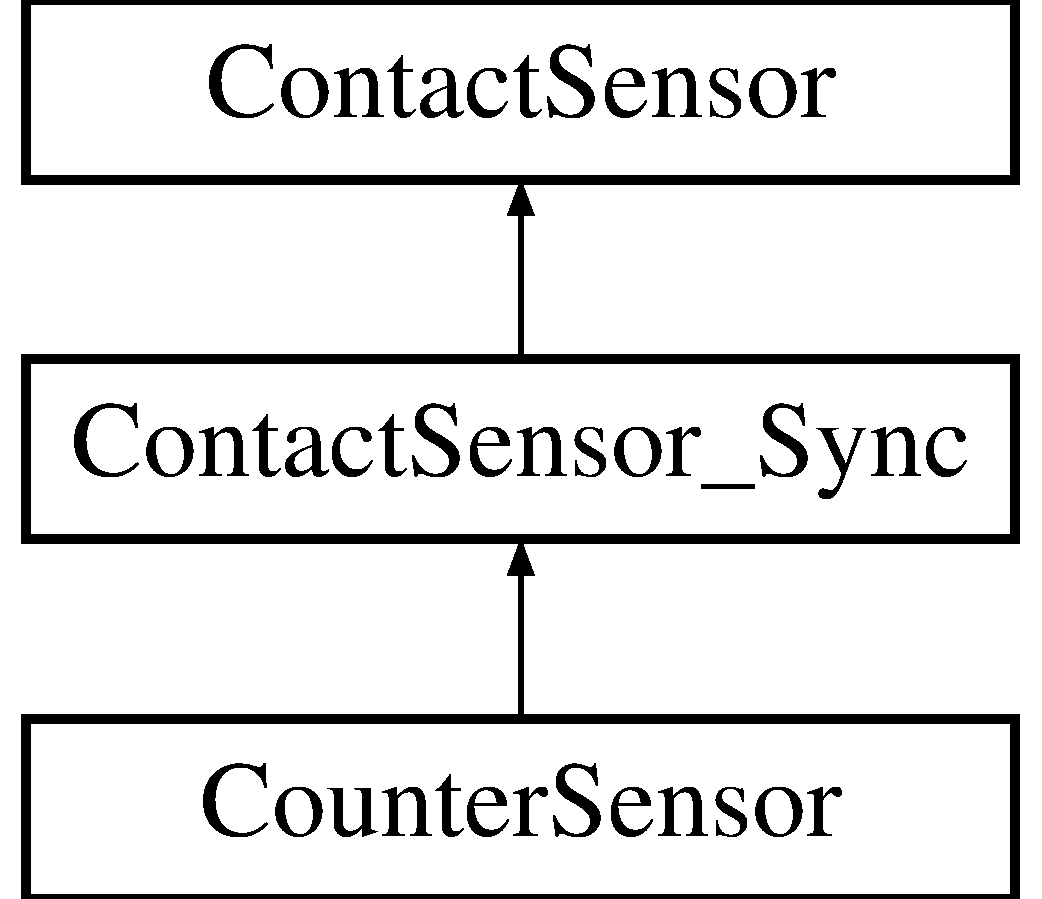
\includegraphics[height=3.000000cm]{classCounterSensor}
\end{center}
\end{figure}
\subsection*{Public Member Functions}
\begin{DoxyCompactItemize}
\item 
\hyperlink{classCounterSensor_a0a7194fc72b5b35feba9ffe7da90d108}{Counter\-Sensor} (int id, b2\-Vec2 position, float32 radius, b2\-Filter filter, b2\-World $\ast$world)
\item 
void \hyperlink{classCounterSensor_a1763f5725f88b507e8c03149d236ad1f}{update\-Counter} ()
\begin{DoxyCompactList}\small\item\em Increase counter by one unit. \end{DoxyCompactList}\item 
void \hyperlink{classCounterSensor_a43e99153ba1e398d66bdc1b1f5bc349d}{draw\-Label} ()
\begin{DoxyCompactList}\small\item\em Draw sensor label. \end{DoxyCompactList}\item 
signed int \hyperlink{classCounterSensor_aec52d1f6a0e52eaa61d356d9f15b665a}{get} ()
\begin{DoxyCompactList}\small\item\em Return the state of the sensor. \end{DoxyCompactList}\end{DoxyCompactItemize}
\subsection*{Public Attributes}
\begin{DoxyCompactItemize}
\item 
signed int \hyperlink{classCounterSensor_a813a9db83bb2930730655a4df647746a}{m\-\_\-counter}
\begin{DoxyCompactList}\small\item\em Stores the number of registered collisions. \end{DoxyCompactList}\end{DoxyCompactItemize}


\subsection{Detailed Description}
Count the number of collisions. 

This is used to measure how far a the conveyor-\/belt has traveled.  

\subsection{Constructor \& Destructor Documentation}
\hypertarget{classCounterSensor_a0a7194fc72b5b35feba9ffe7da90d108}{\index{Counter\-Sensor@{Counter\-Sensor}!Counter\-Sensor@{Counter\-Sensor}}
\index{Counter\-Sensor@{Counter\-Sensor}!CounterSensor@{Counter\-Sensor}}
\subsubsection[{Counter\-Sensor}]{\setlength{\rightskip}{0pt plus 5cm}Counter\-Sensor\-::\-Counter\-Sensor (
\begin{DoxyParamCaption}
\item[{int}]{id, }
\item[{b2\-Vec2}]{position, }
\item[{float32}]{radius, }
\item[{b2\-Filter}]{filter, }
\item[{b2\-World $\ast$}]{world}
\end{DoxyParamCaption}
)}}\label{classCounterSensor_a0a7194fc72b5b35feba9ffe7da90d108}


\subsection{Member Function Documentation}
\hypertarget{classCounterSensor_a43e99153ba1e398d66bdc1b1f5bc349d}{\index{Counter\-Sensor@{Counter\-Sensor}!draw\-Label@{draw\-Label}}
\index{draw\-Label@{draw\-Label}!CounterSensor@{Counter\-Sensor}}
\subsubsection[{draw\-Label}]{\setlength{\rightskip}{0pt plus 5cm}void Counter\-Sensor\-::draw\-Label (
\begin{DoxyParamCaption}
{}
\end{DoxyParamCaption}
)\hspace{0.3cm}{\ttfamily [virtual]}}}\label{classCounterSensor_a43e99153ba1e398d66bdc1b1f5bc349d}


Draw sensor label. 



Reimplemented from \hyperlink{classContactSensor__Sync_ae7eed2d2ee0e58940426d4701f695481}{Contact\-Sensor\-\_\-\-Sync}.

\hypertarget{classCounterSensor_aec52d1f6a0e52eaa61d356d9f15b665a}{\index{Counter\-Sensor@{Counter\-Sensor}!get@{get}}
\index{get@{get}!CounterSensor@{Counter\-Sensor}}
\subsubsection[{get}]{\setlength{\rightskip}{0pt plus 5cm}signed int Counter\-Sensor\-::get (
\begin{DoxyParamCaption}
{}
\end{DoxyParamCaption}
)\hspace{0.3cm}{\ttfamily [inline]}, {\ttfamily [virtual]}}}\label{classCounterSensor_aec52d1f6a0e52eaa61d356d9f15b665a}


Return the state of the sensor. 



Reimplemented from \hyperlink{classContactSensor_af616ebea2da4d9fd0dacdf71eb8b32d9}{Contact\-Sensor}.

\hypertarget{classCounterSensor_a1763f5725f88b507e8c03149d236ad1f}{\index{Counter\-Sensor@{Counter\-Sensor}!update\-Counter@{update\-Counter}}
\index{update\-Counter@{update\-Counter}!CounterSensor@{Counter\-Sensor}}
\subsubsection[{update\-Counter}]{\setlength{\rightskip}{0pt plus 5cm}void Counter\-Sensor\-::update\-Counter (
\begin{DoxyParamCaption}
{}
\end{DoxyParamCaption}
)}}\label{classCounterSensor_a1763f5725f88b507e8c03149d236ad1f}


Increase counter by one unit. 



\subsection{Member Data Documentation}
\hypertarget{classCounterSensor_a813a9db83bb2930730655a4df647746a}{\index{Counter\-Sensor@{Counter\-Sensor}!m\-\_\-counter@{m\-\_\-counter}}
\index{m\-\_\-counter@{m\-\_\-counter}!CounterSensor@{Counter\-Sensor}}
\subsubsection[{m\-\_\-counter}]{\setlength{\rightskip}{0pt plus 5cm}signed int Counter\-Sensor\-::m\-\_\-counter}}\label{classCounterSensor_a813a9db83bb2930730655a4df647746a}


Stores the number of registered collisions. 



The documentation for this class was generated from the following files\-:\begin{DoxyCompactItemize}
\item 
\hyperlink{Sensors_8h}{Sensors.\-h}\item 
\hyperlink{Sensors_8cpp}{Sensors.\-cpp}\end{DoxyCompactItemize}

\hypertarget{classDebugDraw}{\section{Debug\-Draw Class Reference}
\label{classDebugDraw}\index{Debug\-Draw@{Debug\-Draw}}
}


{\ttfamily \#include $<$Render.\-h$>$}

Inheritance diagram for Debug\-Draw\-:\begin{figure}[H]
\begin{center}
\leavevmode
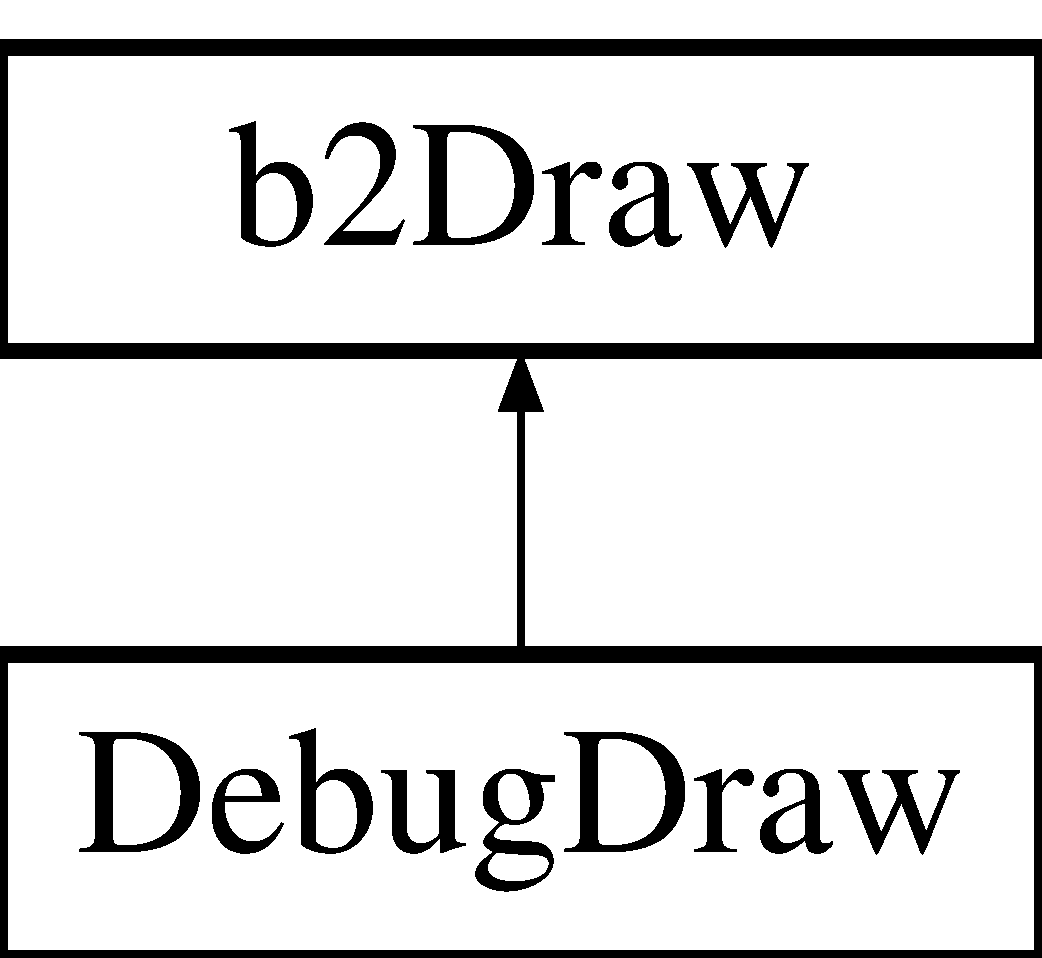
\includegraphics[height=2.000000cm]{classDebugDraw}
\end{center}
\end{figure}
\subsection*{Public Member Functions}
\begin{DoxyCompactItemize}
\item 
void \hyperlink{classDebugDraw_a14ab8cf80799e57df5414db216552962}{Draw\-Polygon} (const b2\-Vec2 $\ast$vertices, int32 vertex\-Count, const b2\-Color \&color)
\item 
void \hyperlink{classDebugDraw_a1562ce91df605efef3cdf300be267cc2}{Draw\-Solid\-Polygon} (const b2\-Vec2 $\ast$vertices, int32 vertex\-Count, const b2\-Color \&color)
\item 
void \hyperlink{classDebugDraw_a5adb064981a67fefe7064820006b673e}{Draw\-Circle} (const b2\-Vec2 \&center, float32 radius, const b2\-Color \&color)
\item 
void \hyperlink{classDebugDraw_a82428519034f36a01941dd19d6108bee}{Draw\-Solid\-Circle} (const b2\-Vec2 \&center, float32 radius, const b2\-Vec2 \&axis, const b2\-Color \&color)
\item 
void \hyperlink{classDebugDraw_a69927caae41d26f23dea336a1269ee4e}{Draw\-Segment} (const b2\-Vec2 \&p1, const b2\-Vec2 \&p2, const b2\-Color \&color)
\item 
void \hyperlink{classDebugDraw_a6f61d333e6e76865ec4a6099ab31ae75}{Draw\-Transform} (const b2\-Transform \&xf)
\item 
void \hyperlink{classDebugDraw_a1f9c99b818e21078a53d11a5ca6e2c79}{Draw\-Point} (const b2\-Vec2 \&p, float32 size, const b2\-Color \&color)
\item 
void \hyperlink{classDebugDraw_a395164a66033cc6e3b7fb596a67f2ea4}{Draw\-String} (int x, int y, const char $\ast$string,...)
\item 
void \hyperlink{classDebugDraw_a9a2a74e510bac791747b2b7badf750b9}{Draw\-A\-A\-B\-B} (b2\-A\-A\-B\-B $\ast$aabb, const b2\-Color \&color)
\end{DoxyCompactItemize}


\subsection{Member Function Documentation}
\hypertarget{classDebugDraw_a9a2a74e510bac791747b2b7badf750b9}{\index{Debug\-Draw@{Debug\-Draw}!Draw\-A\-A\-B\-B@{Draw\-A\-A\-B\-B}}
\index{Draw\-A\-A\-B\-B@{Draw\-A\-A\-B\-B}!DebugDraw@{Debug\-Draw}}
\subsubsection[{Draw\-A\-A\-B\-B}]{\setlength{\rightskip}{0pt plus 5cm}void Debug\-Draw\-::\-Draw\-A\-A\-B\-B (
\begin{DoxyParamCaption}
\item[{b2\-A\-A\-B\-B $\ast$}]{aabb, }
\item[{const b2\-Color \&}]{color}
\end{DoxyParamCaption}
)}}\label{classDebugDraw_a9a2a74e510bac791747b2b7badf750b9}
\hypertarget{classDebugDraw_a5adb064981a67fefe7064820006b673e}{\index{Debug\-Draw@{Debug\-Draw}!Draw\-Circle@{Draw\-Circle}}
\index{Draw\-Circle@{Draw\-Circle}!DebugDraw@{Debug\-Draw}}
\subsubsection[{Draw\-Circle}]{\setlength{\rightskip}{0pt plus 5cm}void Debug\-Draw\-::\-Draw\-Circle (
\begin{DoxyParamCaption}
\item[{const b2\-Vec2 \&}]{center, }
\item[{float32}]{radius, }
\item[{const b2\-Color \&}]{color}
\end{DoxyParamCaption}
)}}\label{classDebugDraw_a5adb064981a67fefe7064820006b673e}
\hypertarget{classDebugDraw_a1f9c99b818e21078a53d11a5ca6e2c79}{\index{Debug\-Draw@{Debug\-Draw}!Draw\-Point@{Draw\-Point}}
\index{Draw\-Point@{Draw\-Point}!DebugDraw@{Debug\-Draw}}
\subsubsection[{Draw\-Point}]{\setlength{\rightskip}{0pt plus 5cm}void Debug\-Draw\-::\-Draw\-Point (
\begin{DoxyParamCaption}
\item[{const b2\-Vec2 \&}]{p, }
\item[{float32}]{size, }
\item[{const b2\-Color \&}]{color}
\end{DoxyParamCaption}
)}}\label{classDebugDraw_a1f9c99b818e21078a53d11a5ca6e2c79}
\hypertarget{classDebugDraw_a14ab8cf80799e57df5414db216552962}{\index{Debug\-Draw@{Debug\-Draw}!Draw\-Polygon@{Draw\-Polygon}}
\index{Draw\-Polygon@{Draw\-Polygon}!DebugDraw@{Debug\-Draw}}
\subsubsection[{Draw\-Polygon}]{\setlength{\rightskip}{0pt plus 5cm}void Debug\-Draw\-::\-Draw\-Polygon (
\begin{DoxyParamCaption}
\item[{const b2\-Vec2 $\ast$}]{vertices, }
\item[{int32}]{vertex\-Count, }
\item[{const b2\-Color \&}]{color}
\end{DoxyParamCaption}
)}}\label{classDebugDraw_a14ab8cf80799e57df5414db216552962}
\hypertarget{classDebugDraw_a69927caae41d26f23dea336a1269ee4e}{\index{Debug\-Draw@{Debug\-Draw}!Draw\-Segment@{Draw\-Segment}}
\index{Draw\-Segment@{Draw\-Segment}!DebugDraw@{Debug\-Draw}}
\subsubsection[{Draw\-Segment}]{\setlength{\rightskip}{0pt plus 5cm}void Debug\-Draw\-::\-Draw\-Segment (
\begin{DoxyParamCaption}
\item[{const b2\-Vec2 \&}]{p1, }
\item[{const b2\-Vec2 \&}]{p2, }
\item[{const b2\-Color \&}]{color}
\end{DoxyParamCaption}
)}}\label{classDebugDraw_a69927caae41d26f23dea336a1269ee4e}
\hypertarget{classDebugDraw_a82428519034f36a01941dd19d6108bee}{\index{Debug\-Draw@{Debug\-Draw}!Draw\-Solid\-Circle@{Draw\-Solid\-Circle}}
\index{Draw\-Solid\-Circle@{Draw\-Solid\-Circle}!DebugDraw@{Debug\-Draw}}
\subsubsection[{Draw\-Solid\-Circle}]{\setlength{\rightskip}{0pt plus 5cm}void Debug\-Draw\-::\-Draw\-Solid\-Circle (
\begin{DoxyParamCaption}
\item[{const b2\-Vec2 \&}]{center, }
\item[{float32}]{radius, }
\item[{const b2\-Vec2 \&}]{axis, }
\item[{const b2\-Color \&}]{color}
\end{DoxyParamCaption}
)}}\label{classDebugDraw_a82428519034f36a01941dd19d6108bee}
\hypertarget{classDebugDraw_a1562ce91df605efef3cdf300be267cc2}{\index{Debug\-Draw@{Debug\-Draw}!Draw\-Solid\-Polygon@{Draw\-Solid\-Polygon}}
\index{Draw\-Solid\-Polygon@{Draw\-Solid\-Polygon}!DebugDraw@{Debug\-Draw}}
\subsubsection[{Draw\-Solid\-Polygon}]{\setlength{\rightskip}{0pt plus 5cm}void Debug\-Draw\-::\-Draw\-Solid\-Polygon (
\begin{DoxyParamCaption}
\item[{const b2\-Vec2 $\ast$}]{vertices, }
\item[{int32}]{vertex\-Count, }
\item[{const b2\-Color \&}]{color}
\end{DoxyParamCaption}
)}}\label{classDebugDraw_a1562ce91df605efef3cdf300be267cc2}
\hypertarget{classDebugDraw_a395164a66033cc6e3b7fb596a67f2ea4}{\index{Debug\-Draw@{Debug\-Draw}!Draw\-String@{Draw\-String}}
\index{Draw\-String@{Draw\-String}!DebugDraw@{Debug\-Draw}}
\subsubsection[{Draw\-String}]{\setlength{\rightskip}{0pt plus 5cm}void Debug\-Draw\-::\-Draw\-String (
\begin{DoxyParamCaption}
\item[{int}]{x, }
\item[{int}]{y, }
\item[{const char $\ast$}]{string, }
\item[{}]{...}
\end{DoxyParamCaption}
)}}\label{classDebugDraw_a395164a66033cc6e3b7fb596a67f2ea4}
\hypertarget{classDebugDraw_a6f61d333e6e76865ec4a6099ab31ae75}{\index{Debug\-Draw@{Debug\-Draw}!Draw\-Transform@{Draw\-Transform}}
\index{Draw\-Transform@{Draw\-Transform}!DebugDraw@{Debug\-Draw}}
\subsubsection[{Draw\-Transform}]{\setlength{\rightskip}{0pt plus 5cm}void Debug\-Draw\-::\-Draw\-Transform (
\begin{DoxyParamCaption}
\item[{const b2\-Transform \&}]{xf}
\end{DoxyParamCaption}
)}}\label{classDebugDraw_a6f61d333e6e76865ec4a6099ab31ae75}


The documentation for this class was generated from the following files\-:\begin{DoxyCompactItemize}
\item 
\hyperlink{Render_8h}{Render.\-h}\item 
\hyperlink{Render_8cpp}{Render.\-cpp}\end{DoxyCompactItemize}

\hypertarget{classDestructionListener}{\section{Destruction\-Listener Class Reference}
\label{classDestructionListener}\index{Destruction\-Listener@{Destruction\-Listener}}
}


{\ttfamily \#include $<$Simulator\-Page.\-h$>$}

Inheritance diagram for Destruction\-Listener\-:\begin{figure}[H]
\begin{center}
\leavevmode
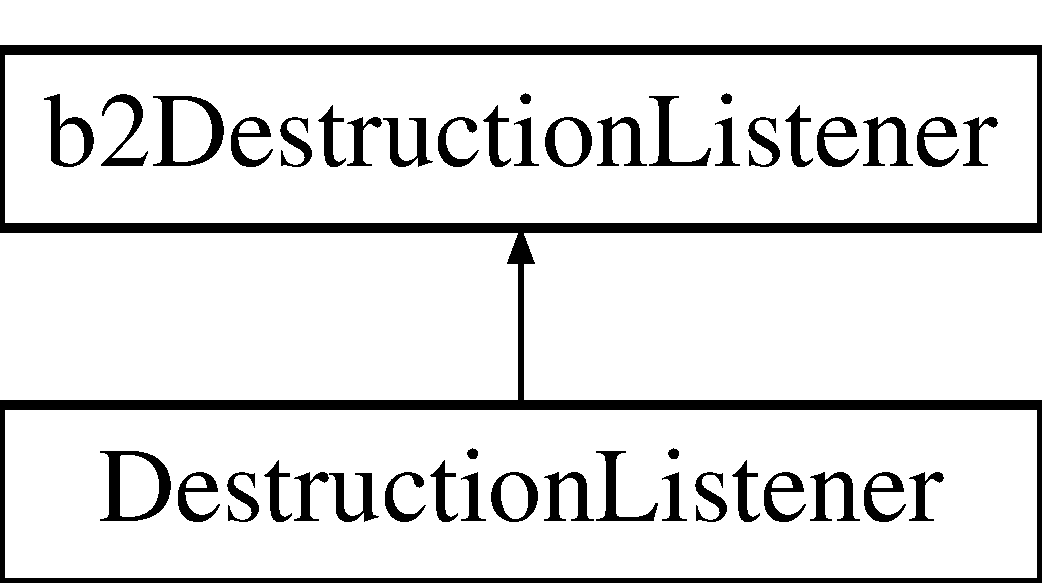
\includegraphics[height=2.000000cm]{classDestructionListener}
\end{center}
\end{figure}
\subsection*{Public Member Functions}
\begin{DoxyCompactItemize}
\item 
void \hyperlink{classDestructionListener_a51b3b045b48c33fbfaa0182b329d5d49}{Say\-Goodbye} (b2\-Fixture $\ast$fixture)
\item 
void \hyperlink{classDestructionListener_a55627bd55b8816d66e0f3d85a75c0552}{Say\-Goodbye} (b2\-Joint $\ast$joint)
\end{DoxyCompactItemize}
\subsection*{Public Attributes}
\begin{DoxyCompactItemize}
\item 
\hyperlink{classSimulatorPage}{Simulator\-Page} $\ast$ \hyperlink{classDestructionListener_a23c82561bcb7e2b9b9c9c71b46e4d62a}{simulator\-Page}
\end{DoxyCompactItemize}


\subsection{Member Function Documentation}
\hypertarget{classDestructionListener_a51b3b045b48c33fbfaa0182b329d5d49}{\index{Destruction\-Listener@{Destruction\-Listener}!Say\-Goodbye@{Say\-Goodbye}}
\index{Say\-Goodbye@{Say\-Goodbye}!DestructionListener@{Destruction\-Listener}}
\subsubsection[{Say\-Goodbye}]{\setlength{\rightskip}{0pt plus 5cm}void Destruction\-Listener\-::\-Say\-Goodbye (
\begin{DoxyParamCaption}
\item[{b2\-Fixture $\ast$}]{fixture}
\end{DoxyParamCaption}
)\hspace{0.3cm}{\ttfamily [inline]}}}\label{classDestructionListener_a51b3b045b48c33fbfaa0182b329d5d49}
\hypertarget{classDestructionListener_a55627bd55b8816d66e0f3d85a75c0552}{\index{Destruction\-Listener@{Destruction\-Listener}!Say\-Goodbye@{Say\-Goodbye}}
\index{Say\-Goodbye@{Say\-Goodbye}!DestructionListener@{Destruction\-Listener}}
\subsubsection[{Say\-Goodbye}]{\setlength{\rightskip}{0pt plus 5cm}void Destruction\-Listener\-::\-Say\-Goodbye (
\begin{DoxyParamCaption}
\item[{b2\-Joint $\ast$}]{joint}
\end{DoxyParamCaption}
)}}\label{classDestructionListener_a55627bd55b8816d66e0f3d85a75c0552}


\subsection{Member Data Documentation}
\hypertarget{classDestructionListener_a23c82561bcb7e2b9b9c9c71b46e4d62a}{\index{Destruction\-Listener@{Destruction\-Listener}!simulator\-Page@{simulator\-Page}}
\index{simulator\-Page@{simulator\-Page}!DestructionListener@{Destruction\-Listener}}
\subsubsection[{simulator\-Page}]{\setlength{\rightskip}{0pt plus 5cm}{\bf Simulator\-Page}$\ast$ Destruction\-Listener\-::simulator\-Page}}\label{classDestructionListener_a23c82561bcb7e2b9b9c9c71b46e4d62a}


The documentation for this class was generated from the following files\-:\begin{DoxyCompactItemize}
\item 
\hyperlink{SimulatorPage_8h}{Simulator\-Page.\-h}\item 
\hyperlink{SimulatorPage_8cpp}{Simulator\-Page.\-cpp}\end{DoxyCompactItemize}

\hypertarget{classJointActuatorPrismaticBinary}{\section{Joint\-Actuator\-Prismatic\-Binary Class Reference}
\label{classJointActuatorPrismaticBinary}\index{Joint\-Actuator\-Prismatic\-Binary@{Joint\-Actuator\-Prismatic\-Binary}}
}


Switch a prismatic joint between the two extremal states.  




{\ttfamily \#include $<$Actuators.\-h$>$}

Inheritance diagram for Joint\-Actuator\-Prismatic\-Binary\-:\begin{figure}[H]
\begin{center}
\leavevmode
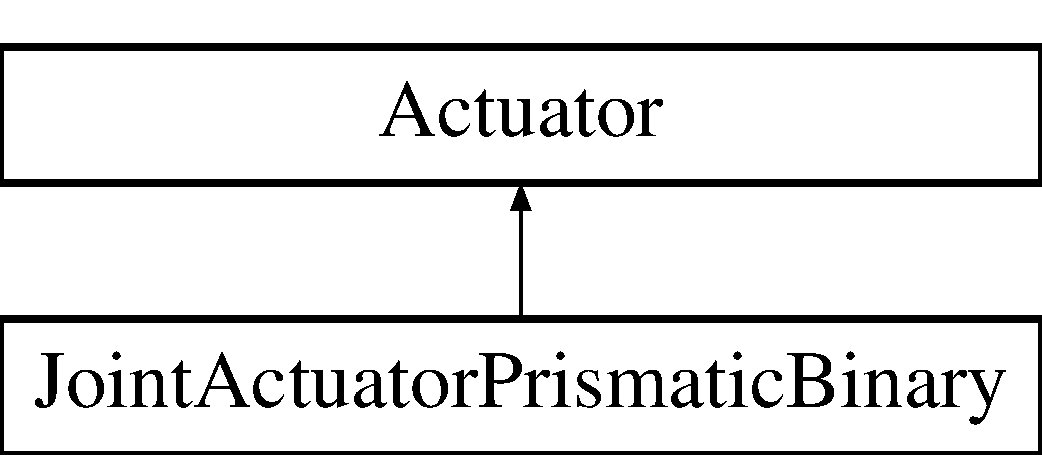
\includegraphics[height=2.000000cm]{classJointActuatorPrismaticBinary}
\end{center}
\end{figure}
\subsection*{Public Member Functions}
\begin{DoxyCompactItemize}
\item 
\hyperlink{classJointActuatorPrismaticBinary_aaaf871b53bc2e1c60088a9cd3a385949}{Joint\-Actuator\-Prismatic\-Binary} (int id, b2\-Joint $\ast$joint)
\item 
void \hyperlink{classJointActuatorPrismaticBinary_a78d1185c3762bb4301f31f0619cded7a}{set} (signed int value)
\item 
void \hyperlink{classJointActuatorPrismaticBinary_af5ea6bfc6b9e45d42b98d76d0a6c48ab}{set\-Speed} (float32 speed)
\item 
void \hyperlink{classJointActuatorPrismaticBinary_a2c4cd26a0ae47850eca1047ba078a654}{draw\-Label} ()
\end{DoxyCompactItemize}
\subsection*{Public Attributes}
\begin{DoxyCompactItemize}
\item 
b2\-Joint $\ast$ \hyperlink{classJointActuatorPrismaticBinary_acfe11f8fb117fa9257067367fcf9a8bc}{m\-\_\-joint}
\item 
float32 \hyperlink{classJointActuatorPrismaticBinary_aeeaabbbb710800d517ddfa34c7c68ded}{m\-\_\-speed}
\end{DoxyCompactItemize}


\subsection{Detailed Description}
Switch a prismatic joint between the two extremal states. 

\subsection{Constructor \& Destructor Documentation}
\hypertarget{classJointActuatorPrismaticBinary_aaaf871b53bc2e1c60088a9cd3a385949}{\index{Joint\-Actuator\-Prismatic\-Binary@{Joint\-Actuator\-Prismatic\-Binary}!Joint\-Actuator\-Prismatic\-Binary@{Joint\-Actuator\-Prismatic\-Binary}}
\index{Joint\-Actuator\-Prismatic\-Binary@{Joint\-Actuator\-Prismatic\-Binary}!JointActuatorPrismaticBinary@{Joint\-Actuator\-Prismatic\-Binary}}
\subsubsection[{Joint\-Actuator\-Prismatic\-Binary}]{\setlength{\rightskip}{0pt plus 5cm}Joint\-Actuator\-Prismatic\-Binary\-::\-Joint\-Actuator\-Prismatic\-Binary (
\begin{DoxyParamCaption}
\item[{int}]{id, }
\item[{b2\-Joint $\ast$}]{joint}
\end{DoxyParamCaption}
)}}\label{classJointActuatorPrismaticBinary_aaaf871b53bc2e1c60088a9cd3a385949}


\subsection{Member Function Documentation}
\hypertarget{classJointActuatorPrismaticBinary_a2c4cd26a0ae47850eca1047ba078a654}{\index{Joint\-Actuator\-Prismatic\-Binary@{Joint\-Actuator\-Prismatic\-Binary}!draw\-Label@{draw\-Label}}
\index{draw\-Label@{draw\-Label}!JointActuatorPrismaticBinary@{Joint\-Actuator\-Prismatic\-Binary}}
\subsubsection[{draw\-Label}]{\setlength{\rightskip}{0pt plus 5cm}void Joint\-Actuator\-Prismatic\-Binary\-::draw\-Label (
\begin{DoxyParamCaption}
{}
\end{DoxyParamCaption}
)\hspace{0.3cm}{\ttfamily [virtual]}}}\label{classJointActuatorPrismaticBinary_a2c4cd26a0ae47850eca1047ba078a654}


Reimplemented from \hyperlink{classActuator_aaa39a438315ac34dbb1a4237bf70ff99}{Actuator}.

\hypertarget{classJointActuatorPrismaticBinary_a78d1185c3762bb4301f31f0619cded7a}{\index{Joint\-Actuator\-Prismatic\-Binary@{Joint\-Actuator\-Prismatic\-Binary}!set@{set}}
\index{set@{set}!JointActuatorPrismaticBinary@{Joint\-Actuator\-Prismatic\-Binary}}
\subsubsection[{set}]{\setlength{\rightskip}{0pt plus 5cm}void Joint\-Actuator\-Prismatic\-Binary\-::set (
\begin{DoxyParamCaption}
\item[{signed int}]{value}
\end{DoxyParamCaption}
)\hspace{0.3cm}{\ttfamily [virtual]}}}\label{classJointActuatorPrismaticBinary_a78d1185c3762bb4301f31f0619cded7a}


Reimplemented from \hyperlink{classActuator_a6281019cccd4034ab2cf7071defecf70}{Actuator}.

\hypertarget{classJointActuatorPrismaticBinary_af5ea6bfc6b9e45d42b98d76d0a6c48ab}{\index{Joint\-Actuator\-Prismatic\-Binary@{Joint\-Actuator\-Prismatic\-Binary}!set\-Speed@{set\-Speed}}
\index{set\-Speed@{set\-Speed}!JointActuatorPrismaticBinary@{Joint\-Actuator\-Prismatic\-Binary}}
\subsubsection[{set\-Speed}]{\setlength{\rightskip}{0pt plus 5cm}void Joint\-Actuator\-Prismatic\-Binary\-::set\-Speed (
\begin{DoxyParamCaption}
\item[{float32}]{speed}
\end{DoxyParamCaption}
)\hspace{0.3cm}{\ttfamily [inline]}}}\label{classJointActuatorPrismaticBinary_af5ea6bfc6b9e45d42b98d76d0a6c48ab}


\subsection{Member Data Documentation}
\hypertarget{classJointActuatorPrismaticBinary_acfe11f8fb117fa9257067367fcf9a8bc}{\index{Joint\-Actuator\-Prismatic\-Binary@{Joint\-Actuator\-Prismatic\-Binary}!m\-\_\-joint@{m\-\_\-joint}}
\index{m\-\_\-joint@{m\-\_\-joint}!JointActuatorPrismaticBinary@{Joint\-Actuator\-Prismatic\-Binary}}
\subsubsection[{m\-\_\-joint}]{\setlength{\rightskip}{0pt plus 5cm}b2\-Joint$\ast$ Joint\-Actuator\-Prismatic\-Binary\-::m\-\_\-joint}}\label{classJointActuatorPrismaticBinary_acfe11f8fb117fa9257067367fcf9a8bc}
\hypertarget{classJointActuatorPrismaticBinary_aeeaabbbb710800d517ddfa34c7c68ded}{\index{Joint\-Actuator\-Prismatic\-Binary@{Joint\-Actuator\-Prismatic\-Binary}!m\-\_\-speed@{m\-\_\-speed}}
\index{m\-\_\-speed@{m\-\_\-speed}!JointActuatorPrismaticBinary@{Joint\-Actuator\-Prismatic\-Binary}}
\subsubsection[{m\-\_\-speed}]{\setlength{\rightskip}{0pt plus 5cm}float32 Joint\-Actuator\-Prismatic\-Binary\-::m\-\_\-speed}}\label{classJointActuatorPrismaticBinary_aeeaabbbb710800d517ddfa34c7c68ded}


The documentation for this class was generated from the following files\-:\begin{DoxyCompactItemize}
\item 
\hyperlink{Actuators_8h}{Actuators.\-h}\item 
\hyperlink{Actuators_8cpp}{Actuators.\-cpp}\end{DoxyCompactItemize}

\hypertarget{classJointActuatorPrismaticRange}{\section{Joint\-Actuator\-Prismatic\-Range Class Reference}
\label{classJointActuatorPrismaticRange}\index{Joint\-Actuator\-Prismatic\-Range@{Joint\-Actuator\-Prismatic\-Range}}
}


Run a prismatic joint at an arbitrary constant speed.  




{\ttfamily \#include $<$Actuators.\-h$>$}

Inheritance diagram for Joint\-Actuator\-Prismatic\-Range\-:\begin{figure}[H]
\begin{center}
\leavevmode
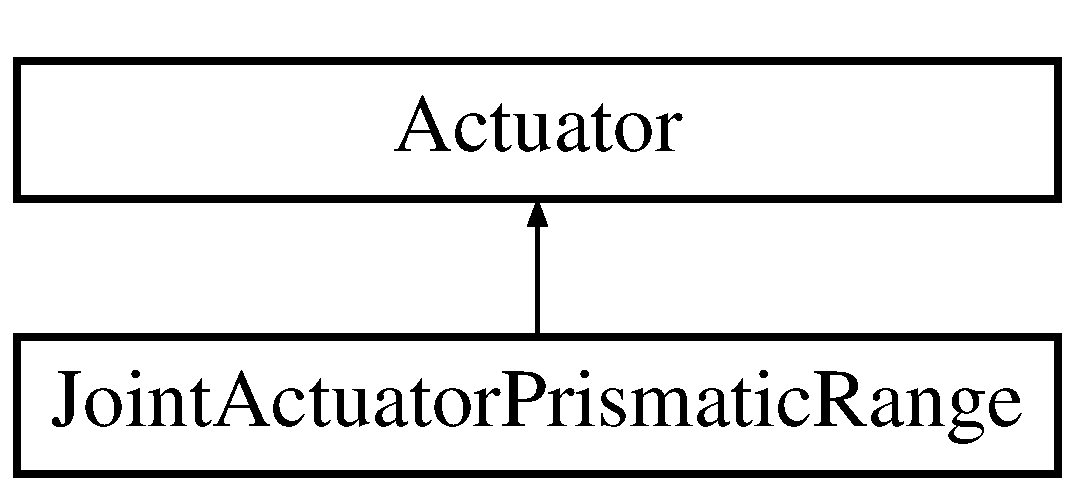
\includegraphics[height=2.000000cm]{classJointActuatorPrismaticRange}
\end{center}
\end{figure}
\subsection*{Public Member Functions}
\begin{DoxyCompactItemize}
\item 
\hyperlink{classJointActuatorPrismaticRange_ad1e60e9b3b976eeaa276d9194cd30695}{Joint\-Actuator\-Prismatic\-Range} (int id, b2\-Joint $\ast$joint)
\item 
void \hyperlink{classJointActuatorPrismaticRange_a6df9efdb8bf3cea3cffefa977a6f4c02}{set} (signed int value)
\item 
void \hyperlink{classJointActuatorPrismaticRange_a9daa027177e5bd6c0296b3cf4a76e9ab}{draw\-Label} ()
\end{DoxyCompactItemize}
\subsection*{Public Attributes}
\begin{DoxyCompactItemize}
\item 
b2\-Joint $\ast$ \hyperlink{classJointActuatorPrismaticRange_ab272c14737ab32f88291d3999cbbf398}{m\-\_\-joint}
\end{DoxyCompactItemize}


\subsection{Detailed Description}
Run a prismatic joint at an arbitrary constant speed. 

\subsection{Constructor \& Destructor Documentation}
\hypertarget{classJointActuatorPrismaticRange_ad1e60e9b3b976eeaa276d9194cd30695}{\index{Joint\-Actuator\-Prismatic\-Range@{Joint\-Actuator\-Prismatic\-Range}!Joint\-Actuator\-Prismatic\-Range@{Joint\-Actuator\-Prismatic\-Range}}
\index{Joint\-Actuator\-Prismatic\-Range@{Joint\-Actuator\-Prismatic\-Range}!JointActuatorPrismaticRange@{Joint\-Actuator\-Prismatic\-Range}}
\subsubsection[{Joint\-Actuator\-Prismatic\-Range}]{\setlength{\rightskip}{0pt plus 5cm}Joint\-Actuator\-Prismatic\-Range\-::\-Joint\-Actuator\-Prismatic\-Range (
\begin{DoxyParamCaption}
\item[{int}]{id, }
\item[{b2\-Joint $\ast$}]{joint}
\end{DoxyParamCaption}
)}}\label{classJointActuatorPrismaticRange_ad1e60e9b3b976eeaa276d9194cd30695}


\subsection{Member Function Documentation}
\hypertarget{classJointActuatorPrismaticRange_a9daa027177e5bd6c0296b3cf4a76e9ab}{\index{Joint\-Actuator\-Prismatic\-Range@{Joint\-Actuator\-Prismatic\-Range}!draw\-Label@{draw\-Label}}
\index{draw\-Label@{draw\-Label}!JointActuatorPrismaticRange@{Joint\-Actuator\-Prismatic\-Range}}
\subsubsection[{draw\-Label}]{\setlength{\rightskip}{0pt plus 5cm}void Joint\-Actuator\-Prismatic\-Range\-::draw\-Label (
\begin{DoxyParamCaption}
{}
\end{DoxyParamCaption}
)\hspace{0.3cm}{\ttfamily [virtual]}}}\label{classJointActuatorPrismaticRange_a9daa027177e5bd6c0296b3cf4a76e9ab}


Reimplemented from \hyperlink{classActuator_aaa39a438315ac34dbb1a4237bf70ff99}{Actuator}.

\hypertarget{classJointActuatorPrismaticRange_a6df9efdb8bf3cea3cffefa977a6f4c02}{\index{Joint\-Actuator\-Prismatic\-Range@{Joint\-Actuator\-Prismatic\-Range}!set@{set}}
\index{set@{set}!JointActuatorPrismaticRange@{Joint\-Actuator\-Prismatic\-Range}}
\subsubsection[{set}]{\setlength{\rightskip}{0pt plus 5cm}void Joint\-Actuator\-Prismatic\-Range\-::set (
\begin{DoxyParamCaption}
\item[{signed int}]{value}
\end{DoxyParamCaption}
)\hspace{0.3cm}{\ttfamily [virtual]}}}\label{classJointActuatorPrismaticRange_a6df9efdb8bf3cea3cffefa977a6f4c02}


Reimplemented from \hyperlink{classActuator_a6281019cccd4034ab2cf7071defecf70}{Actuator}.



\subsection{Member Data Documentation}
\hypertarget{classJointActuatorPrismaticRange_ab272c14737ab32f88291d3999cbbf398}{\index{Joint\-Actuator\-Prismatic\-Range@{Joint\-Actuator\-Prismatic\-Range}!m\-\_\-joint@{m\-\_\-joint}}
\index{m\-\_\-joint@{m\-\_\-joint}!JointActuatorPrismaticRange@{Joint\-Actuator\-Prismatic\-Range}}
\subsubsection[{m\-\_\-joint}]{\setlength{\rightskip}{0pt plus 5cm}b2\-Joint$\ast$ Joint\-Actuator\-Prismatic\-Range\-::m\-\_\-joint}}\label{classJointActuatorPrismaticRange_ab272c14737ab32f88291d3999cbbf398}


The documentation for this class was generated from the following files\-:\begin{DoxyCompactItemize}
\item 
\hyperlink{Actuators_8h}{Actuators.\-h}\item 
\hyperlink{Actuators_8cpp}{Actuators.\-cpp}\end{DoxyCompactItemize}

\hypertarget{classJointActuatorPrismaticStep}{\section{Joint\-Actuator\-Prismatic\-Step Class Reference}
\label{classJointActuatorPrismaticStep}\index{Joint\-Actuator\-Prismatic\-Step@{Joint\-Actuator\-Prismatic\-Step}}
}


Run a prismatic joint an arbitrary number of steps.  




{\ttfamily \#include $<$Actuators.\-h$>$}

Inheritance diagram for Joint\-Actuator\-Prismatic\-Step\-:\begin{figure}[H]
\begin{center}
\leavevmode
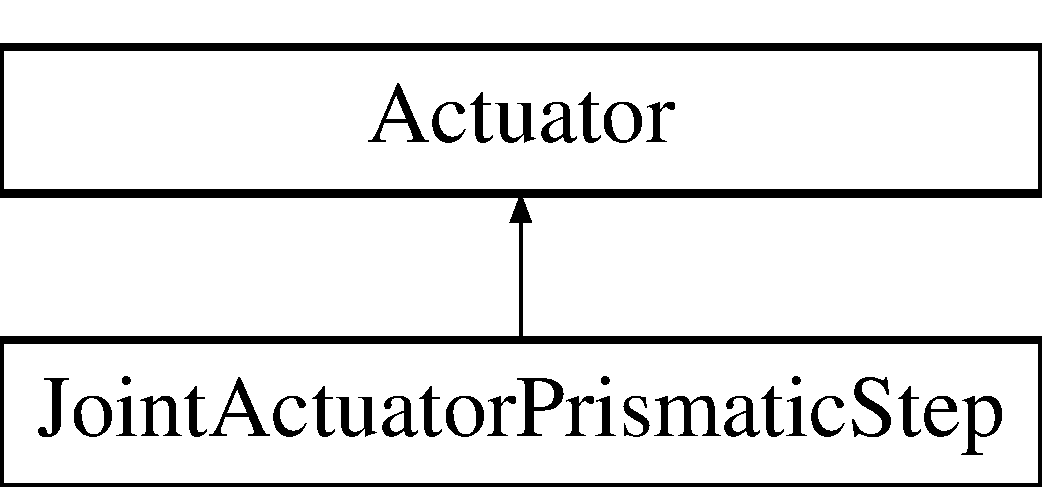
\includegraphics[height=2.000000cm]{classJointActuatorPrismaticStep}
\end{center}
\end{figure}
\subsection*{Public Member Functions}
\begin{DoxyCompactItemize}
\item 
\hyperlink{classJointActuatorPrismaticStep_a15f20c8424d7bc4e226ea428a3d316fa}{Joint\-Actuator\-Prismatic\-Step} (int id, b2\-Joint $\ast$joint)
\item 
void \hyperlink{classJointActuatorPrismaticStep_ace7839e236e16848375f963697ac408a}{set} (signed int value)
\item 
void \hyperlink{classJointActuatorPrismaticStep_aecbb187fd46eb1e197a34bcd54aaf4d4}{draw\-Label} ()
\item 
void \hyperlink{classJointActuatorPrismaticStep_a30a61d48a3719b5d0390be85b7445883}{run} ()
\end{DoxyCompactItemize}
\subsection*{Public Attributes}
\begin{DoxyCompactItemize}
\item 
b2\-Joint $\ast$ \hyperlink{classJointActuatorPrismaticStep_a0b0796c249dd6cecd0c0616a80885ab9}{m\-\_\-joint}
\item 
b2\-Vec2 \hyperlink{classJointActuatorPrismaticStep_a48a004131133ef920d4bed5912519ffc}{m\-\_\-start\-Pos}
\item 
b2\-Vec2 \hyperlink{classJointActuatorPrismaticStep_a13ea9ddc095eaf6e30d0dee871025b29}{m\-\_\-current\-Pos}
\item 
float32 \hyperlink{classJointActuatorPrismaticStep_aa3c0a7f6384201a79b14b681d0b9f274}{m\-\_\-max\-Displacement}
\item 
signed int \hyperlink{classJointActuatorPrismaticStep_a92c61c564dbfc17830ec4109be54f008}{m\-\_\-value}
\end{DoxyCompactItemize}


\subsection{Detailed Description}
Run a prismatic joint an arbitrary number of steps. 

\subsection{Constructor \& Destructor Documentation}
\hypertarget{classJointActuatorPrismaticStep_a15f20c8424d7bc4e226ea428a3d316fa}{\index{Joint\-Actuator\-Prismatic\-Step@{Joint\-Actuator\-Prismatic\-Step}!Joint\-Actuator\-Prismatic\-Step@{Joint\-Actuator\-Prismatic\-Step}}
\index{Joint\-Actuator\-Prismatic\-Step@{Joint\-Actuator\-Prismatic\-Step}!JointActuatorPrismaticStep@{Joint\-Actuator\-Prismatic\-Step}}
\subsubsection[{Joint\-Actuator\-Prismatic\-Step}]{\setlength{\rightskip}{0pt plus 5cm}Joint\-Actuator\-Prismatic\-Step\-::\-Joint\-Actuator\-Prismatic\-Step (
\begin{DoxyParamCaption}
\item[{int}]{id, }
\item[{b2\-Joint $\ast$}]{joint}
\end{DoxyParamCaption}
)}}\label{classJointActuatorPrismaticStep_a15f20c8424d7bc4e226ea428a3d316fa}


\subsection{Member Function Documentation}
\hypertarget{classJointActuatorPrismaticStep_aecbb187fd46eb1e197a34bcd54aaf4d4}{\index{Joint\-Actuator\-Prismatic\-Step@{Joint\-Actuator\-Prismatic\-Step}!draw\-Label@{draw\-Label}}
\index{draw\-Label@{draw\-Label}!JointActuatorPrismaticStep@{Joint\-Actuator\-Prismatic\-Step}}
\subsubsection[{draw\-Label}]{\setlength{\rightskip}{0pt plus 5cm}void Joint\-Actuator\-Prismatic\-Step\-::draw\-Label (
\begin{DoxyParamCaption}
{}
\end{DoxyParamCaption}
)\hspace{0.3cm}{\ttfamily [virtual]}}}\label{classJointActuatorPrismaticStep_aecbb187fd46eb1e197a34bcd54aaf4d4}


Reimplemented from \hyperlink{classActuator_aaa39a438315ac34dbb1a4237bf70ff99}{Actuator}.

\hypertarget{classJointActuatorPrismaticStep_a30a61d48a3719b5d0390be85b7445883}{\index{Joint\-Actuator\-Prismatic\-Step@{Joint\-Actuator\-Prismatic\-Step}!run@{run}}
\index{run@{run}!JointActuatorPrismaticStep@{Joint\-Actuator\-Prismatic\-Step}}
\subsubsection[{run}]{\setlength{\rightskip}{0pt plus 5cm}void Joint\-Actuator\-Prismatic\-Step\-::run (
\begin{DoxyParamCaption}
{}
\end{DoxyParamCaption}
)\hspace{0.3cm}{\ttfamily [virtual]}}}\label{classJointActuatorPrismaticStep_a30a61d48a3719b5d0390be85b7445883}


Reimplemented from \hyperlink{classActuator_aabe48a4249a91a4cd1b964001fe754fc}{Actuator}.

\hypertarget{classJointActuatorPrismaticStep_ace7839e236e16848375f963697ac408a}{\index{Joint\-Actuator\-Prismatic\-Step@{Joint\-Actuator\-Prismatic\-Step}!set@{set}}
\index{set@{set}!JointActuatorPrismaticStep@{Joint\-Actuator\-Prismatic\-Step}}
\subsubsection[{set}]{\setlength{\rightskip}{0pt plus 5cm}void Joint\-Actuator\-Prismatic\-Step\-::set (
\begin{DoxyParamCaption}
\item[{signed int}]{value}
\end{DoxyParamCaption}
)\hspace{0.3cm}{\ttfamily [virtual]}}}\label{classJointActuatorPrismaticStep_ace7839e236e16848375f963697ac408a}


Reimplemented from \hyperlink{classActuator_a6281019cccd4034ab2cf7071defecf70}{Actuator}.



\subsection{Member Data Documentation}
\hypertarget{classJointActuatorPrismaticStep_a13ea9ddc095eaf6e30d0dee871025b29}{\index{Joint\-Actuator\-Prismatic\-Step@{Joint\-Actuator\-Prismatic\-Step}!m\-\_\-current\-Pos@{m\-\_\-current\-Pos}}
\index{m\-\_\-current\-Pos@{m\-\_\-current\-Pos}!JointActuatorPrismaticStep@{Joint\-Actuator\-Prismatic\-Step}}
\subsubsection[{m\-\_\-current\-Pos}]{\setlength{\rightskip}{0pt plus 5cm}b2\-Vec2 Joint\-Actuator\-Prismatic\-Step\-::m\-\_\-current\-Pos}}\label{classJointActuatorPrismaticStep_a13ea9ddc095eaf6e30d0dee871025b29}
\hypertarget{classJointActuatorPrismaticStep_a0b0796c249dd6cecd0c0616a80885ab9}{\index{Joint\-Actuator\-Prismatic\-Step@{Joint\-Actuator\-Prismatic\-Step}!m\-\_\-joint@{m\-\_\-joint}}
\index{m\-\_\-joint@{m\-\_\-joint}!JointActuatorPrismaticStep@{Joint\-Actuator\-Prismatic\-Step}}
\subsubsection[{m\-\_\-joint}]{\setlength{\rightskip}{0pt plus 5cm}b2\-Joint$\ast$ Joint\-Actuator\-Prismatic\-Step\-::m\-\_\-joint}}\label{classJointActuatorPrismaticStep_a0b0796c249dd6cecd0c0616a80885ab9}
\hypertarget{classJointActuatorPrismaticStep_aa3c0a7f6384201a79b14b681d0b9f274}{\index{Joint\-Actuator\-Prismatic\-Step@{Joint\-Actuator\-Prismatic\-Step}!m\-\_\-max\-Displacement@{m\-\_\-max\-Displacement}}
\index{m\-\_\-max\-Displacement@{m\-\_\-max\-Displacement}!JointActuatorPrismaticStep@{Joint\-Actuator\-Prismatic\-Step}}
\subsubsection[{m\-\_\-max\-Displacement}]{\setlength{\rightskip}{0pt plus 5cm}float32 Joint\-Actuator\-Prismatic\-Step\-::m\-\_\-max\-Displacement}}\label{classJointActuatorPrismaticStep_aa3c0a7f6384201a79b14b681d0b9f274}
\hypertarget{classJointActuatorPrismaticStep_a48a004131133ef920d4bed5912519ffc}{\index{Joint\-Actuator\-Prismatic\-Step@{Joint\-Actuator\-Prismatic\-Step}!m\-\_\-start\-Pos@{m\-\_\-start\-Pos}}
\index{m\-\_\-start\-Pos@{m\-\_\-start\-Pos}!JointActuatorPrismaticStep@{Joint\-Actuator\-Prismatic\-Step}}
\subsubsection[{m\-\_\-start\-Pos}]{\setlength{\rightskip}{0pt plus 5cm}b2\-Vec2 Joint\-Actuator\-Prismatic\-Step\-::m\-\_\-start\-Pos}}\label{classJointActuatorPrismaticStep_a48a004131133ef920d4bed5912519ffc}
\hypertarget{classJointActuatorPrismaticStep_a92c61c564dbfc17830ec4109be54f008}{\index{Joint\-Actuator\-Prismatic\-Step@{Joint\-Actuator\-Prismatic\-Step}!m\-\_\-value@{m\-\_\-value}}
\index{m\-\_\-value@{m\-\_\-value}!JointActuatorPrismaticStep@{Joint\-Actuator\-Prismatic\-Step}}
\subsubsection[{m\-\_\-value}]{\setlength{\rightskip}{0pt plus 5cm}signed int Joint\-Actuator\-Prismatic\-Step\-::m\-\_\-value}}\label{classJointActuatorPrismaticStep_a92c61c564dbfc17830ec4109be54f008}


The documentation for this class was generated from the following files\-:\begin{DoxyCompactItemize}
\item 
\hyperlink{Actuators_8h}{Actuators.\-h}\item 
\hyperlink{Actuators_8cpp}{Actuators.\-cpp}\end{DoxyCompactItemize}

\hypertarget{classJointActuatorRevoluteStep}{\section{Joint\-Actuator\-Revolute\-Step Class Reference}
\label{classJointActuatorRevoluteStep}\index{Joint\-Actuator\-Revolute\-Step@{Joint\-Actuator\-Revolute\-Step}}
}


Turn a revolute joint an arbitrary angle.  




{\ttfamily \#include $<$Actuators.\-h$>$}

Inheritance diagram for Joint\-Actuator\-Revolute\-Step\-:\begin{figure}[H]
\begin{center}
\leavevmode
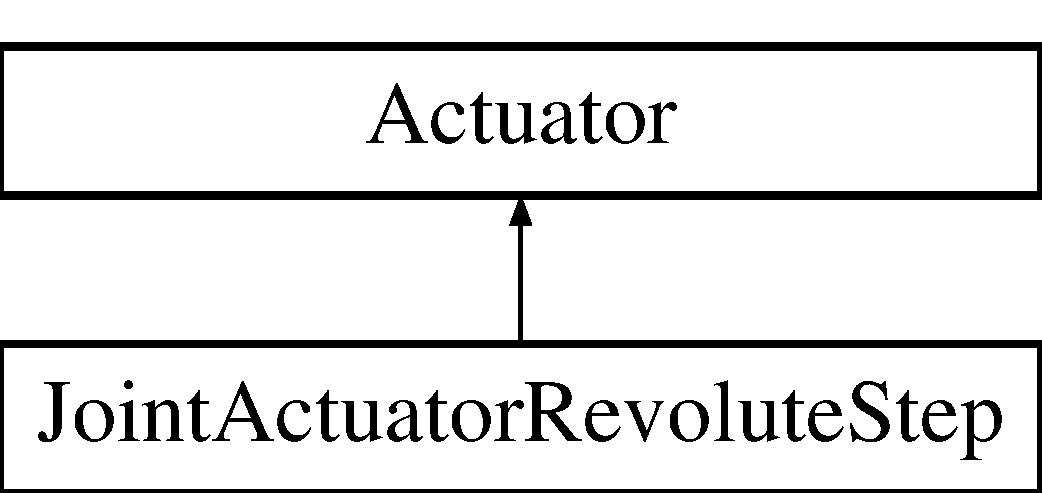
\includegraphics[height=2.000000cm]{classJointActuatorRevoluteStep}
\end{center}
\end{figure}
\subsection*{Public Member Functions}
\begin{DoxyCompactItemize}
\item 
\hyperlink{classJointActuatorRevoluteStep_a10d7586a8bfd9afdee5d1d32d2da4360}{Joint\-Actuator\-Revolute\-Step} (int id, b2\-Joint $\ast$joint)
\item 
void \hyperlink{classJointActuatorRevoluteStep_af72ade5873ae6b2816f1f7c89bf95971}{set} (signed int value)
\item 
void \hyperlink{classJointActuatorRevoluteStep_ab390783e9b495488afa09e8f29aee6d9}{draw\-Label} ()
\item 
void \hyperlink{classJointActuatorRevoluteStep_a6445fceda983f3fd1f0b280bb03a66af}{run} ()
\end{DoxyCompactItemize}
\subsection*{Public Attributes}
\begin{DoxyCompactItemize}
\item 
b2\-Joint $\ast$ \hyperlink{classJointActuatorRevoluteStep_a0b4484f5b13d01dcb0960cdd8f74cc0c}{m\-\_\-joint}
\item 
float32 \hyperlink{classJointActuatorRevoluteStep_aecca63a8d37534fcad4e12524a0c19a8}{m\-\_\-start\-Angle}
\item 
float32 \hyperlink{classJointActuatorRevoluteStep_a0df1b8e4adca3517b2a1aa3fa60c047c}{m\-\_\-current\-Angle}
\item 
float32 \hyperlink{classJointActuatorRevoluteStep_a708c8fd9fbc8ddf9eed1adf9029214b4}{m\-\_\-max\-Rotation}
\item 
signed int \hyperlink{classJointActuatorRevoluteStep_ae9c426c866c77fde187ee3cddb3a6ca4}{m\-\_\-value}
\end{DoxyCompactItemize}


\subsection{Detailed Description}
Turn a revolute joint an arbitrary angle. 

\subsection{Constructor \& Destructor Documentation}
\hypertarget{classJointActuatorRevoluteStep_a10d7586a8bfd9afdee5d1d32d2da4360}{\index{Joint\-Actuator\-Revolute\-Step@{Joint\-Actuator\-Revolute\-Step}!Joint\-Actuator\-Revolute\-Step@{Joint\-Actuator\-Revolute\-Step}}
\index{Joint\-Actuator\-Revolute\-Step@{Joint\-Actuator\-Revolute\-Step}!JointActuatorRevoluteStep@{Joint\-Actuator\-Revolute\-Step}}
\subsubsection[{Joint\-Actuator\-Revolute\-Step}]{\setlength{\rightskip}{0pt plus 5cm}Joint\-Actuator\-Revolute\-Step\-::\-Joint\-Actuator\-Revolute\-Step (
\begin{DoxyParamCaption}
\item[{int}]{id, }
\item[{b2\-Joint $\ast$}]{joint}
\end{DoxyParamCaption}
)}}\label{classJointActuatorRevoluteStep_a10d7586a8bfd9afdee5d1d32d2da4360}


\subsection{Member Function Documentation}
\hypertarget{classJointActuatorRevoluteStep_ab390783e9b495488afa09e8f29aee6d9}{\index{Joint\-Actuator\-Revolute\-Step@{Joint\-Actuator\-Revolute\-Step}!draw\-Label@{draw\-Label}}
\index{draw\-Label@{draw\-Label}!JointActuatorRevoluteStep@{Joint\-Actuator\-Revolute\-Step}}
\subsubsection[{draw\-Label}]{\setlength{\rightskip}{0pt plus 5cm}void Joint\-Actuator\-Revolute\-Step\-::draw\-Label (
\begin{DoxyParamCaption}
{}
\end{DoxyParamCaption}
)\hspace{0.3cm}{\ttfamily [virtual]}}}\label{classJointActuatorRevoluteStep_ab390783e9b495488afa09e8f29aee6d9}


Reimplemented from \hyperlink{classActuator_aaa39a438315ac34dbb1a4237bf70ff99}{Actuator}.

\hypertarget{classJointActuatorRevoluteStep_a6445fceda983f3fd1f0b280bb03a66af}{\index{Joint\-Actuator\-Revolute\-Step@{Joint\-Actuator\-Revolute\-Step}!run@{run}}
\index{run@{run}!JointActuatorRevoluteStep@{Joint\-Actuator\-Revolute\-Step}}
\subsubsection[{run}]{\setlength{\rightskip}{0pt plus 5cm}void Joint\-Actuator\-Revolute\-Step\-::run (
\begin{DoxyParamCaption}
{}
\end{DoxyParamCaption}
)\hspace{0.3cm}{\ttfamily [virtual]}}}\label{classJointActuatorRevoluteStep_a6445fceda983f3fd1f0b280bb03a66af}


Reimplemented from \hyperlink{classActuator_aabe48a4249a91a4cd1b964001fe754fc}{Actuator}.

\hypertarget{classJointActuatorRevoluteStep_af72ade5873ae6b2816f1f7c89bf95971}{\index{Joint\-Actuator\-Revolute\-Step@{Joint\-Actuator\-Revolute\-Step}!set@{set}}
\index{set@{set}!JointActuatorRevoluteStep@{Joint\-Actuator\-Revolute\-Step}}
\subsubsection[{set}]{\setlength{\rightskip}{0pt plus 5cm}void Joint\-Actuator\-Revolute\-Step\-::set (
\begin{DoxyParamCaption}
\item[{signed int}]{value}
\end{DoxyParamCaption}
)\hspace{0.3cm}{\ttfamily [virtual]}}}\label{classJointActuatorRevoluteStep_af72ade5873ae6b2816f1f7c89bf95971}


Reimplemented from \hyperlink{classActuator_a6281019cccd4034ab2cf7071defecf70}{Actuator}.



\subsection{Member Data Documentation}
\hypertarget{classJointActuatorRevoluteStep_a0df1b8e4adca3517b2a1aa3fa60c047c}{\index{Joint\-Actuator\-Revolute\-Step@{Joint\-Actuator\-Revolute\-Step}!m\-\_\-current\-Angle@{m\-\_\-current\-Angle}}
\index{m\-\_\-current\-Angle@{m\-\_\-current\-Angle}!JointActuatorRevoluteStep@{Joint\-Actuator\-Revolute\-Step}}
\subsubsection[{m\-\_\-current\-Angle}]{\setlength{\rightskip}{0pt plus 5cm}float32 Joint\-Actuator\-Revolute\-Step\-::m\-\_\-current\-Angle}}\label{classJointActuatorRevoluteStep_a0df1b8e4adca3517b2a1aa3fa60c047c}
\hypertarget{classJointActuatorRevoluteStep_a0b4484f5b13d01dcb0960cdd8f74cc0c}{\index{Joint\-Actuator\-Revolute\-Step@{Joint\-Actuator\-Revolute\-Step}!m\-\_\-joint@{m\-\_\-joint}}
\index{m\-\_\-joint@{m\-\_\-joint}!JointActuatorRevoluteStep@{Joint\-Actuator\-Revolute\-Step}}
\subsubsection[{m\-\_\-joint}]{\setlength{\rightskip}{0pt plus 5cm}b2\-Joint$\ast$ Joint\-Actuator\-Revolute\-Step\-::m\-\_\-joint}}\label{classJointActuatorRevoluteStep_a0b4484f5b13d01dcb0960cdd8f74cc0c}
\hypertarget{classJointActuatorRevoluteStep_a708c8fd9fbc8ddf9eed1adf9029214b4}{\index{Joint\-Actuator\-Revolute\-Step@{Joint\-Actuator\-Revolute\-Step}!m\-\_\-max\-Rotation@{m\-\_\-max\-Rotation}}
\index{m\-\_\-max\-Rotation@{m\-\_\-max\-Rotation}!JointActuatorRevoluteStep@{Joint\-Actuator\-Revolute\-Step}}
\subsubsection[{m\-\_\-max\-Rotation}]{\setlength{\rightskip}{0pt plus 5cm}float32 Joint\-Actuator\-Revolute\-Step\-::m\-\_\-max\-Rotation}}\label{classJointActuatorRevoluteStep_a708c8fd9fbc8ddf9eed1adf9029214b4}
\hypertarget{classJointActuatorRevoluteStep_aecca63a8d37534fcad4e12524a0c19a8}{\index{Joint\-Actuator\-Revolute\-Step@{Joint\-Actuator\-Revolute\-Step}!m\-\_\-start\-Angle@{m\-\_\-start\-Angle}}
\index{m\-\_\-start\-Angle@{m\-\_\-start\-Angle}!JointActuatorRevoluteStep@{Joint\-Actuator\-Revolute\-Step}}
\subsubsection[{m\-\_\-start\-Angle}]{\setlength{\rightskip}{0pt plus 5cm}float32 Joint\-Actuator\-Revolute\-Step\-::m\-\_\-start\-Angle}}\label{classJointActuatorRevoluteStep_aecca63a8d37534fcad4e12524a0c19a8}
\hypertarget{classJointActuatorRevoluteStep_ae9c426c866c77fde187ee3cddb3a6ca4}{\index{Joint\-Actuator\-Revolute\-Step@{Joint\-Actuator\-Revolute\-Step}!m\-\_\-value@{m\-\_\-value}}
\index{m\-\_\-value@{m\-\_\-value}!JointActuatorRevoluteStep@{Joint\-Actuator\-Revolute\-Step}}
\subsubsection[{m\-\_\-value}]{\setlength{\rightskip}{0pt plus 5cm}signed int Joint\-Actuator\-Revolute\-Step\-::m\-\_\-value}}\label{classJointActuatorRevoluteStep_ae9c426c866c77fde187ee3cddb3a6ca4}


The documentation for this class was generated from the following files\-:\begin{DoxyCompactItemize}
\item 
\hyperlink{Actuators_8h}{Actuators.\-h}\item 
\hyperlink{Actuators_8cpp}{Actuators.\-cpp}\end{DoxyCompactItemize}

\hypertarget{classLengthSensor}{\section{Length\-Sensor Class Reference}
\label{classLengthSensor}\index{Length\-Sensor@{Length\-Sensor}}
}


Measure length of a colliding Plank-\/instance.  




{\ttfamily \#include $<$Sensors.\-h$>$}

Inheritance diagram for Length\-Sensor\-:\begin{figure}[H]
\begin{center}
\leavevmode
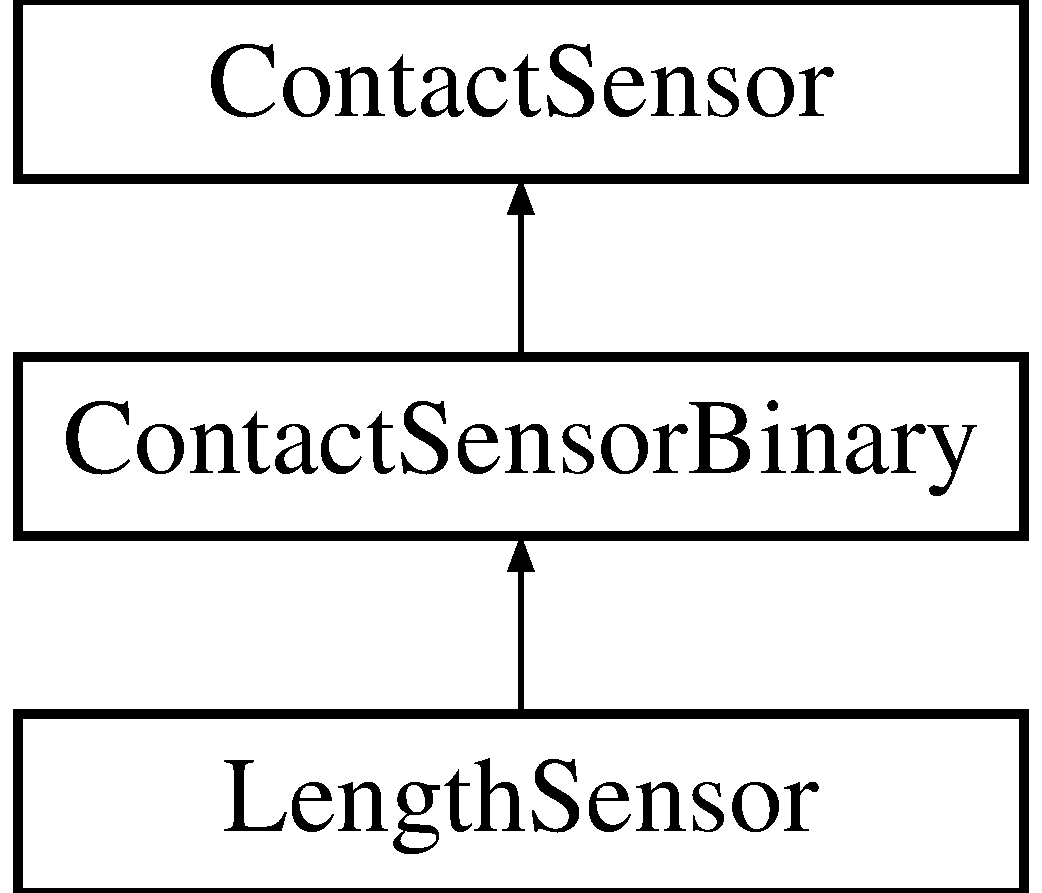
\includegraphics[height=3.000000cm]{classLengthSensor}
\end{center}
\end{figure}
\subsection*{Public Member Functions}
\begin{DoxyCompactItemize}
\item 
\hyperlink{classLengthSensor_aa691f5e5e97607b3f0979379fd958c3b}{Length\-Sensor} (int id, b2\-Vec2 position, float32 radius, b2\-World $\ast$world)
\item 
void \hyperlink{classLengthSensor_aae468465d3ab04b316f7553423feb4ff}{meassure\-Length} (float32 length)
\item 
signed int \hyperlink{classLengthSensor_a90d9ddfdeb189991d274026af6ab8681}{get} ()
\begin{DoxyCompactList}\small\item\em Return the state of the sensor. \end{DoxyCompactList}\end{DoxyCompactItemize}
\subsection*{Public Attributes}
\begin{DoxyCompactItemize}
\item 
signed int \hyperlink{classLengthSensor_a755a8b3fd195e6d20c1898016cc0efa2}{m\-\_\-meassured\-Lenght}
\begin{DoxyCompactList}\small\item\em Store the last measured plank length. \end{DoxyCompactList}\end{DoxyCompactItemize}


\subsection{Detailed Description}
Measure length of a colliding Plank-\/instance. 

\subsection{Constructor \& Destructor Documentation}
\hypertarget{classLengthSensor_aa691f5e5e97607b3f0979379fd958c3b}{\index{Length\-Sensor@{Length\-Sensor}!Length\-Sensor@{Length\-Sensor}}
\index{Length\-Sensor@{Length\-Sensor}!LengthSensor@{Length\-Sensor}}
\subsubsection[{Length\-Sensor}]{\setlength{\rightskip}{0pt plus 5cm}Length\-Sensor\-::\-Length\-Sensor (
\begin{DoxyParamCaption}
\item[{int}]{id, }
\item[{b2\-Vec2}]{position, }
\item[{float32}]{radius, }
\item[{b2\-World $\ast$}]{world}
\end{DoxyParamCaption}
)}}\label{classLengthSensor_aa691f5e5e97607b3f0979379fd958c3b}


\subsection{Member Function Documentation}
\hypertarget{classLengthSensor_a90d9ddfdeb189991d274026af6ab8681}{\index{Length\-Sensor@{Length\-Sensor}!get@{get}}
\index{get@{get}!LengthSensor@{Length\-Sensor}}
\subsubsection[{get}]{\setlength{\rightskip}{0pt plus 5cm}signed int Length\-Sensor\-::get (
\begin{DoxyParamCaption}
{}
\end{DoxyParamCaption}
)\hspace{0.3cm}{\ttfamily [inline]}, {\ttfamily [virtual]}}}\label{classLengthSensor_a90d9ddfdeb189991d274026af6ab8681}


Return the state of the sensor. 



Reimplemented from \hyperlink{classContactSensorBinary_a68e856e0d580f91f518099874f8c226b}{Contact\-Sensor\-Binary}.

\hypertarget{classLengthSensor_aae468465d3ab04b316f7553423feb4ff}{\index{Length\-Sensor@{Length\-Sensor}!meassure\-Length@{meassure\-Length}}
\index{meassure\-Length@{meassure\-Length}!LengthSensor@{Length\-Sensor}}
\subsubsection[{meassure\-Length}]{\setlength{\rightskip}{0pt plus 5cm}void Length\-Sensor\-::meassure\-Length (
\begin{DoxyParamCaption}
\item[{float32}]{length}
\end{DoxyParamCaption}
)}}\label{classLengthSensor_aae468465d3ab04b316f7553423feb4ff}


\subsection{Member Data Documentation}
\hypertarget{classLengthSensor_a755a8b3fd195e6d20c1898016cc0efa2}{\index{Length\-Sensor@{Length\-Sensor}!m\-\_\-meassured\-Lenght@{m\-\_\-meassured\-Lenght}}
\index{m\-\_\-meassured\-Lenght@{m\-\_\-meassured\-Lenght}!LengthSensor@{Length\-Sensor}}
\subsubsection[{m\-\_\-meassured\-Lenght}]{\setlength{\rightskip}{0pt plus 5cm}signed int Length\-Sensor\-::m\-\_\-meassured\-Lenght}}\label{classLengthSensor_a755a8b3fd195e6d20c1898016cc0efa2}


Store the last measured plank length. 



The documentation for this class was generated from the following files\-:\begin{DoxyCompactItemize}
\item 
\hyperlink{Sensors_8h}{Sensors.\-h}\item 
\hyperlink{Sensors_8cpp}{Sensors.\-cpp}\end{DoxyCompactItemize}

\hypertarget{classMedbringerkUserData}{\section{Medbringerk\-User\-Data Class Reference}
\label{classMedbringerkUserData}\index{Medbringerk\-User\-Data@{Medbringerk\-User\-Data}}
}


Identify a b2\-Fixture as a \char`\"{}medbringer\char`\"{}.  




{\ttfamily \#include $<$User\-Data.\-h$>$}

Inheritance diagram for Medbringerk\-User\-Data\-:\begin{figure}[H]
\begin{center}
\leavevmode
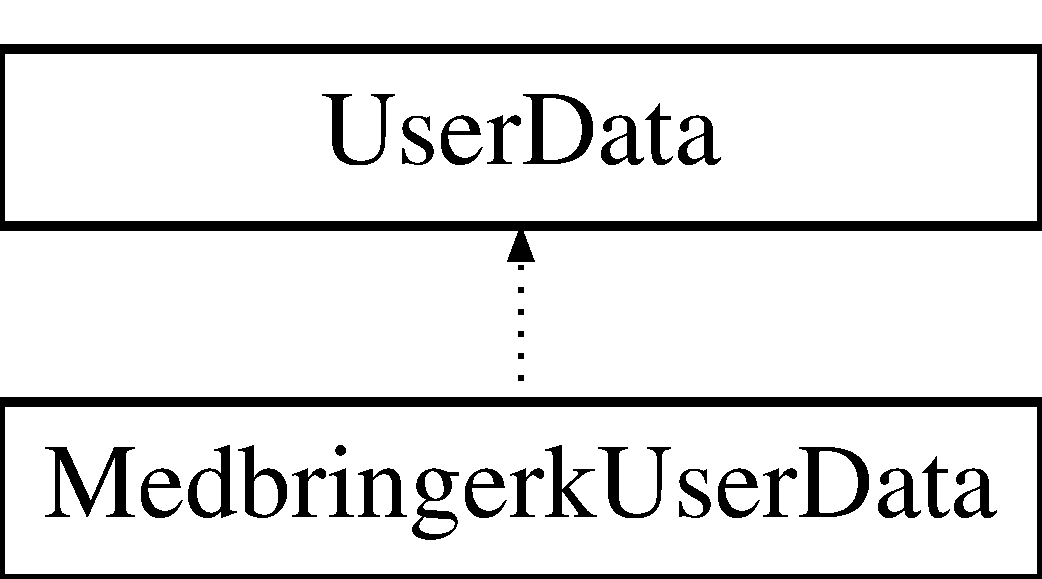
\includegraphics[height=2.000000cm]{classMedbringerkUserData}
\end{center}
\end{figure}
\subsection*{Public Member Functions}
\begin{DoxyCompactItemize}
\item 
\hyperlink{classMedbringerkUserData_a7de96419398d38f5a9d70cc121741dc9}{Medbringerk\-User\-Data} ()
\end{DoxyCompactItemize}
\subsection*{Additional Inherited Members}


\subsection{Detailed Description}
Identify a b2\-Fixture as a \char`\"{}medbringer\char`\"{}. 

Each \char`\"{}medbringers\char`\"{} b2\-Fixture points to an instance of this class. 

\subsection{Constructor \& Destructor Documentation}
\hypertarget{classMedbringerkUserData_a7de96419398d38f5a9d70cc121741dc9}{\index{Medbringerk\-User\-Data@{Medbringerk\-User\-Data}!Medbringerk\-User\-Data@{Medbringerk\-User\-Data}}
\index{Medbringerk\-User\-Data@{Medbringerk\-User\-Data}!MedbringerkUserData@{Medbringerk\-User\-Data}}
\subsubsection[{Medbringerk\-User\-Data}]{\setlength{\rightskip}{0pt plus 5cm}Medbringerk\-User\-Data\-::\-Medbringerk\-User\-Data (
\begin{DoxyParamCaption}
{}
\end{DoxyParamCaption}
)\hspace{0.3cm}{\ttfamily [inline]}}}\label{classMedbringerkUserData_a7de96419398d38f5a9d70cc121741dc9}


The documentation for this class was generated from the following file\-:\begin{DoxyCompactItemize}
\item 
\hyperlink{UserData_8h}{User\-Data.\-h}\end{DoxyCompactItemize}

\hypertarget{classPackage}{\section{Package Class Reference}
\label{classPackage}\index{Package@{Package}}
}


Represent Package-\/objects.  




{\ttfamily \#include $<$Package.\-h$>$}

\subsection*{Public Member Functions}
\begin{DoxyCompactItemize}
\item 
\hyperlink{classPackage_a22b244832bfd2023aeefb40b9b53636e}{Package} (b2\-Vec2 position, b2\-World $\ast$world)
\item 
\hyperlink{classPackage_af9b48c577bb6045c2cbc97d09f76e973}{$\sim$\-Package} ()
\item 
float32 \hyperlink{classPackage_a0721952ecd3c3b61d5e12d2d32bb00f0}{get\-Plank\-Thickness} ()
\item 
float32 \hyperlink{classPackage_a9d32935ea281de4dc12986707a8db71f}{get\-Sprinkle\-Thickness} ()
\item 
void \hyperlink{classPackage_aa4e520d69f6a7d910bc917a8b2a4e2e2}{run\-Sprinkle\-Remover} ()
\begin{DoxyCompactList}\small\item\em Remove sprinkles when outside a predefined circular boundary. \end{DoxyCompactList}\end{DoxyCompactItemize}
\subsection*{Public Attributes}
\begin{DoxyCompactItemize}
\item 
float32 \hyperlink{classPackage_a9dd0955c53dc70f64c0dda77c82022bf}{m\-\_\-plank\-Thickness}
\item 
float32 \hyperlink{classPackage_a6c553d1b7c40cc277a141443789d1dcb}{m\-\_\-sprinkle\-Thickness}
\item 
\hyperlink{classSprinkle}{Sprinkle} $\ast$ \hyperlink{classPackage_a49c8135c0f0f1926e046c0fcd1904e68}{m\-\_\-sprinkle} \mbox{[}7\mbox{]}
\item 
\hyperlink{classPlank}{Plank} $\ast$ \hyperlink{classPackage_a3b902b5536530fd4f66e4cbb2a59fa6f}{m\-\_\-plank} \mbox{[}32\mbox{]}
\end{DoxyCompactItemize}


\subsection{Detailed Description}
Represent Package-\/objects. 

 

\subsection{Constructor \& Destructor Documentation}
\hypertarget{classPackage_a22b244832bfd2023aeefb40b9b53636e}{\index{Package@{Package}!Package@{Package}}
\index{Package@{Package}!Package@{Package}}
\subsubsection[{Package}]{\setlength{\rightskip}{0pt plus 5cm}Package\-::\-Package (
\begin{DoxyParamCaption}
\item[{b2\-Vec2}]{position, }
\item[{b2\-World $\ast$}]{world}
\end{DoxyParamCaption}
)}}\label{classPackage_a22b244832bfd2023aeefb40b9b53636e}
Create a package wherever you want.


\begin{DoxyParams}{Parameters}
{\em position} & Lower left corner of package. \\
\hline
{\em world} & The world in which you want to create the package. \\
\hline
\end{DoxyParams}
\hypertarget{classPackage_af9b48c577bb6045c2cbc97d09f76e973}{\index{Package@{Package}!$\sim$\-Package@{$\sim$\-Package}}
\index{$\sim$\-Package@{$\sim$\-Package}!Package@{Package}}
\subsubsection[{$\sim$\-Package}]{\setlength{\rightskip}{0pt plus 5cm}Package\-::$\sim$\-Package (
\begin{DoxyParamCaption}
{}
\end{DoxyParamCaption}
)}}\label{classPackage_af9b48c577bb6045c2cbc97d09f76e973}


\subsection{Member Function Documentation}
\hypertarget{classPackage_a0721952ecd3c3b61d5e12d2d32bb00f0}{\index{Package@{Package}!get\-Plank\-Thickness@{get\-Plank\-Thickness}}
\index{get\-Plank\-Thickness@{get\-Plank\-Thickness}!Package@{Package}}
\subsubsection[{get\-Plank\-Thickness}]{\setlength{\rightskip}{0pt plus 5cm}float32 Package\-::get\-Plank\-Thickness (
\begin{DoxyParamCaption}
{}
\end{DoxyParamCaption}
)\hspace{0.3cm}{\ttfamily [inline]}}}\label{classPackage_a0721952ecd3c3b61d5e12d2d32bb00f0}
\hypertarget{classPackage_a9d32935ea281de4dc12986707a8db71f}{\index{Package@{Package}!get\-Sprinkle\-Thickness@{get\-Sprinkle\-Thickness}}
\index{get\-Sprinkle\-Thickness@{get\-Sprinkle\-Thickness}!Package@{Package}}
\subsubsection[{get\-Sprinkle\-Thickness}]{\setlength{\rightskip}{0pt plus 5cm}float32 Package\-::get\-Sprinkle\-Thickness (
\begin{DoxyParamCaption}
{}
\end{DoxyParamCaption}
)\hspace{0.3cm}{\ttfamily [inline]}}}\label{classPackage_a9d32935ea281de4dc12986707a8db71f}
\hypertarget{classPackage_aa4e520d69f6a7d910bc917a8b2a4e2e2}{\index{Package@{Package}!run\-Sprinkle\-Remover@{run\-Sprinkle\-Remover}}
\index{run\-Sprinkle\-Remover@{run\-Sprinkle\-Remover}!Package@{Package}}
\subsubsection[{run\-Sprinkle\-Remover}]{\setlength{\rightskip}{0pt plus 5cm}void Package\-::run\-Sprinkle\-Remover (
\begin{DoxyParamCaption}
{}
\end{DoxyParamCaption}
)}}\label{classPackage_aa4e520d69f6a7d910bc917a8b2a4e2e2}


Remove sprinkles when outside a predefined circular boundary. 

Needs to be called continuously. 

\subsection{Member Data Documentation}
\hypertarget{classPackage_a3b902b5536530fd4f66e4cbb2a59fa6f}{\index{Package@{Package}!m\-\_\-plank@{m\-\_\-plank}}
\index{m\-\_\-plank@{m\-\_\-plank}!Package@{Package}}
\subsubsection[{m\-\_\-plank}]{\setlength{\rightskip}{0pt plus 5cm}{\bf Plank}$\ast$ Package\-::m\-\_\-plank\mbox{[}32\mbox{]}}}\label{classPackage_a3b902b5536530fd4f66e4cbb2a59fa6f}
\hypertarget{classPackage_a9dd0955c53dc70f64c0dda77c82022bf}{\index{Package@{Package}!m\-\_\-plank\-Thickness@{m\-\_\-plank\-Thickness}}
\index{m\-\_\-plank\-Thickness@{m\-\_\-plank\-Thickness}!Package@{Package}}
\subsubsection[{m\-\_\-plank\-Thickness}]{\setlength{\rightskip}{0pt plus 5cm}float32 Package\-::m\-\_\-plank\-Thickness}}\label{classPackage_a9dd0955c53dc70f64c0dda77c82022bf}
\hypertarget{classPackage_a49c8135c0f0f1926e046c0fcd1904e68}{\index{Package@{Package}!m\-\_\-sprinkle@{m\-\_\-sprinkle}}
\index{m\-\_\-sprinkle@{m\-\_\-sprinkle}!Package@{Package}}
\subsubsection[{m\-\_\-sprinkle}]{\setlength{\rightskip}{0pt plus 5cm}{\bf Sprinkle}$\ast$ Package\-::m\-\_\-sprinkle\mbox{[}7\mbox{]}}}\label{classPackage_a49c8135c0f0f1926e046c0fcd1904e68}
\hypertarget{classPackage_a6c553d1b7c40cc277a141443789d1dcb}{\index{Package@{Package}!m\-\_\-sprinkle\-Thickness@{m\-\_\-sprinkle\-Thickness}}
\index{m\-\_\-sprinkle\-Thickness@{m\-\_\-sprinkle\-Thickness}!Package@{Package}}
\subsubsection[{m\-\_\-sprinkle\-Thickness}]{\setlength{\rightskip}{0pt plus 5cm}float32 Package\-::m\-\_\-sprinkle\-Thickness}}\label{classPackage_a6c553d1b7c40cc277a141443789d1dcb}


The documentation for this class was generated from the following files\-:\begin{DoxyCompactItemize}
\item 
\hyperlink{Package_8h}{Package.\-h}\item 
\hyperlink{Package_8cpp}{Package.\-cpp}\end{DoxyCompactItemize}

\hypertarget{classPackageInput}{\section{Package\-Input Class Reference}
\label{classPackageInput}\index{Package\-Input@{Package\-Input}}
}


Represent the package input block.  




{\ttfamily \#include $<$Packaging.\-h$>$}

\subsection*{Public Member Functions}
\begin{DoxyCompactItemize}
\item 
\hyperlink{classPackageInput_a2e389eca02f5080d568100127111ebb2}{Package\-Input} (b2\-Vec2 p, float32 length\-Lying\-Beam, float32 thickness\-Lying\-Beam, float32 height\-Standing\-Beam, float32 thickness\-Standing\-Beam, b2\-World $\ast$world)
\item 
b2\-Prismatic\-Joint $\ast$ \hyperlink{classPackageInput_a00aaf542b9486a48271c844f3b1094c4}{get\-Lift\-Joint} ()
\begin{DoxyCompactList}\small\item\em Return pointer to the Lift\-Joint. \end{DoxyCompactList}\item 
b2\-Revolute\-Joint $\ast$ \hyperlink{classPackageInput_a0f3e4bc745c2a7589db8b9fd085616b7}{get\-Rotate\-Joint} ()
\begin{DoxyCompactList}\small\item\em Return pointer to Rotate\-Joint. \end{DoxyCompactList}\item 
b2\-Fixture $\ast$ \hyperlink{classPackageInput_aa09daf2e760c70438acc2a34b7ad4cc6}{get\-Lift\-Sensor\-Fixture} ()
\begin{DoxyCompactList}\small\item\em Return pointer to the Lift-\/sensor Fixture. \end{DoxyCompactList}\item 
\hyperlink{classPackageSource}{Package\-Source} $\ast$ \hyperlink{classPackageInput_a1084874e9c444dbefb167ad3c6e09a53}{get\-Package\-Source} ()
\begin{DoxyCompactList}\small\item\em Return a pointer to the integrated \hyperlink{classPackageSource}{Package\-Source}. \end{DoxyCompactList}\end{DoxyCompactItemize}
\subsection*{Public Attributes}
\begin{DoxyCompactItemize}
\item 
b2\-Prismatic\-Joint $\ast$ \hyperlink{classPackageInput_a3a7aa8124e8800eb96018a358f5fb50c}{m\-\_\-joint\-Lift}
\item 
b2\-Revolute\-Joint $\ast$ \hyperlink{classPackageInput_ad902718752425e44f187926dcbaa69dd}{m\-\_\-joint\-Rotate}
\item 
b2\-Fixture $\ast$ \hyperlink{classPackageInput_a399f8a43d5e938af2dfbcb2c7362af11}{m\-\_\-fixture\-Lift\-Sensor}
\item 
\hyperlink{classPackageSource}{Package\-Source} $\ast$ \hyperlink{classPackageInput_a6d6fb6ba9ae2f514a418be6f136907d0}{m\-\_\-package\-Source}
\end{DoxyCompactItemize}


\subsection{Detailed Description}
Represent the package input block. 

 

\subsection{Constructor \& Destructor Documentation}
\hypertarget{classPackageInput_a2e389eca02f5080d568100127111ebb2}{\index{Package\-Input@{Package\-Input}!Package\-Input@{Package\-Input}}
\index{Package\-Input@{Package\-Input}!PackageInput@{Package\-Input}}
\subsubsection[{Package\-Input}]{\setlength{\rightskip}{0pt plus 5cm}Package\-Input\-::\-Package\-Input (
\begin{DoxyParamCaption}
\item[{b2\-Vec2}]{p, }
\item[{float32}]{length\-Lying\-Beam, }
\item[{float32}]{thickness\-Lying\-Beam, }
\item[{float32}]{height\-Standing\-Beam, }
\item[{float32}]{thickness\-Standing\-Beam, }
\item[{b2\-World $\ast$}]{world}
\end{DoxyParamCaption}
)}}\label{classPackageInput_a2e389eca02f5080d568100127111ebb2}
Construct a Package\-Input-\/instance at any position.


\begin{DoxyParams}{Parameters}
{\em p} & Pivot-\/point of \hyperlink{classPackageInput}{Package\-Input}. \\
\hline
{\em length\-Lying\-Beam} & Length of the lying beam. \\
\hline
{\em thickness\-Lying\-Beam} & Thickness of the lying beam \\
\hline
{\em height\-Standing\-Beam} & Height of the standing beam. \\
\hline
{\em thickness\-Standing\-Beam} & Thickness of the standing beam. \\
\hline
{\em world} & Pointer to the world i which you want to create the Package\-Input-\/instance. \\
\hline
\end{DoxyParams}


\subsection{Member Function Documentation}
\hypertarget{classPackageInput_a00aaf542b9486a48271c844f3b1094c4}{\index{Package\-Input@{Package\-Input}!get\-Lift\-Joint@{get\-Lift\-Joint}}
\index{get\-Lift\-Joint@{get\-Lift\-Joint}!PackageInput@{Package\-Input}}
\subsubsection[{get\-Lift\-Joint}]{\setlength{\rightskip}{0pt plus 5cm}b2\-Prismatic\-Joint$\ast$ Package\-Input\-::get\-Lift\-Joint (
\begin{DoxyParamCaption}
{}
\end{DoxyParamCaption}
)\hspace{0.3cm}{\ttfamily [inline]}}}\label{classPackageInput_a00aaf542b9486a48271c844f3b1094c4}


Return pointer to the Lift\-Joint. 

\hypertarget{classPackageInput_aa09daf2e760c70438acc2a34b7ad4cc6}{\index{Package\-Input@{Package\-Input}!get\-Lift\-Sensor\-Fixture@{get\-Lift\-Sensor\-Fixture}}
\index{get\-Lift\-Sensor\-Fixture@{get\-Lift\-Sensor\-Fixture}!PackageInput@{Package\-Input}}
\subsubsection[{get\-Lift\-Sensor\-Fixture}]{\setlength{\rightskip}{0pt plus 5cm}b2\-Fixture$\ast$ Package\-Input\-::get\-Lift\-Sensor\-Fixture (
\begin{DoxyParamCaption}
{}
\end{DoxyParamCaption}
)\hspace{0.3cm}{\ttfamily [inline]}}}\label{classPackageInput_aa09daf2e760c70438acc2a34b7ad4cc6}


Return pointer to the Lift-\/sensor Fixture. 

\hypertarget{classPackageInput_a1084874e9c444dbefb167ad3c6e09a53}{\index{Package\-Input@{Package\-Input}!get\-Package\-Source@{get\-Package\-Source}}
\index{get\-Package\-Source@{get\-Package\-Source}!PackageInput@{Package\-Input}}
\subsubsection[{get\-Package\-Source}]{\setlength{\rightskip}{0pt plus 5cm}{\bf Package\-Source}$\ast$ Package\-Input\-::get\-Package\-Source (
\begin{DoxyParamCaption}
{}
\end{DoxyParamCaption}
)\hspace{0.3cm}{\ttfamily [inline]}}}\label{classPackageInput_a1084874e9c444dbefb167ad3c6e09a53}


Return a pointer to the integrated \hyperlink{classPackageSource}{Package\-Source}. 

\hypertarget{classPackageInput_a0f3e4bc745c2a7589db8b9fd085616b7}{\index{Package\-Input@{Package\-Input}!get\-Rotate\-Joint@{get\-Rotate\-Joint}}
\index{get\-Rotate\-Joint@{get\-Rotate\-Joint}!PackageInput@{Package\-Input}}
\subsubsection[{get\-Rotate\-Joint}]{\setlength{\rightskip}{0pt plus 5cm}b2\-Revolute\-Joint$\ast$ Package\-Input\-::get\-Rotate\-Joint (
\begin{DoxyParamCaption}
{}
\end{DoxyParamCaption}
)\hspace{0.3cm}{\ttfamily [inline]}}}\label{classPackageInput_a0f3e4bc745c2a7589db8b9fd085616b7}


Return pointer to Rotate\-Joint. 



\subsection{Member Data Documentation}
\hypertarget{classPackageInput_a399f8a43d5e938af2dfbcb2c7362af11}{\index{Package\-Input@{Package\-Input}!m\-\_\-fixture\-Lift\-Sensor@{m\-\_\-fixture\-Lift\-Sensor}}
\index{m\-\_\-fixture\-Lift\-Sensor@{m\-\_\-fixture\-Lift\-Sensor}!PackageInput@{Package\-Input}}
\subsubsection[{m\-\_\-fixture\-Lift\-Sensor}]{\setlength{\rightskip}{0pt plus 5cm}b2\-Fixture$\ast$ Package\-Input\-::m\-\_\-fixture\-Lift\-Sensor}}\label{classPackageInput_a399f8a43d5e938af2dfbcb2c7362af11}
\hypertarget{classPackageInput_a3a7aa8124e8800eb96018a358f5fb50c}{\index{Package\-Input@{Package\-Input}!m\-\_\-joint\-Lift@{m\-\_\-joint\-Lift}}
\index{m\-\_\-joint\-Lift@{m\-\_\-joint\-Lift}!PackageInput@{Package\-Input}}
\subsubsection[{m\-\_\-joint\-Lift}]{\setlength{\rightskip}{0pt plus 5cm}b2\-Prismatic\-Joint$\ast$ Package\-Input\-::m\-\_\-joint\-Lift}}\label{classPackageInput_a3a7aa8124e8800eb96018a358f5fb50c}
\hypertarget{classPackageInput_ad902718752425e44f187926dcbaa69dd}{\index{Package\-Input@{Package\-Input}!m\-\_\-joint\-Rotate@{m\-\_\-joint\-Rotate}}
\index{m\-\_\-joint\-Rotate@{m\-\_\-joint\-Rotate}!PackageInput@{Package\-Input}}
\subsubsection[{m\-\_\-joint\-Rotate}]{\setlength{\rightskip}{0pt plus 5cm}b2\-Revolute\-Joint$\ast$ Package\-Input\-::m\-\_\-joint\-Rotate}}\label{classPackageInput_ad902718752425e44f187926dcbaa69dd}
\hypertarget{classPackageInput_a6d6fb6ba9ae2f514a418be6f136907d0}{\index{Package\-Input@{Package\-Input}!m\-\_\-package\-Source@{m\-\_\-package\-Source}}
\index{m\-\_\-package\-Source@{m\-\_\-package\-Source}!PackageInput@{Package\-Input}}
\subsubsection[{m\-\_\-package\-Source}]{\setlength{\rightskip}{0pt plus 5cm}{\bf Package\-Source}$\ast$ Package\-Input\-::m\-\_\-package\-Source}}\label{classPackageInput_a6d6fb6ba9ae2f514a418be6f136907d0}


The documentation for this class was generated from the following files\-:\begin{DoxyCompactItemize}
\item 
\hyperlink{Packaging_8h}{Packaging.\-h}\item 
\hyperlink{Packaging_8cpp}{Packaging.\-cpp}\end{DoxyCompactItemize}

\hypertarget{classPackageOutput}{\section{Package\-Output Class Reference}
\label{classPackageOutput}\index{Package\-Output@{Package\-Output}}
}


Represent the package output block.  




{\ttfamily \#include $<$Packaging.\-h$>$}

\subsection*{Public Member Functions}
\begin{DoxyCompactItemize}
\item 
\hyperlink{classPackageOutput_a81bd389107afdc3df10c63f29d971458}{Package\-Output} (b2\-Vec2 position, b2\-World $\ast$world)
\begin{DoxyCompactList}\small\item\em Create Package\-Output-\/instance with center of lyingbeam at any position. \end{DoxyCompactList}\item 
b2\-Prismatic\-Joint $\ast$ \hyperlink{classPackageOutput_a1189dbd68b0da4c9a9d52fe8e826d5c3}{get\-Fork\-Joint} ()
\begin{DoxyCompactList}\small\item\em Return pointer to Fork\-Joint. \end{DoxyCompactList}\item 
b2\-Prismatic\-Joint $\ast$ \hyperlink{classPackageOutput_a67d6e0558552cbee8bba8cc360f7eb3c}{get\-Fork\-Base\-Joint} ()
\begin{DoxyCompactList}\small\item\em Return pointer to Fork\-Base\-Joint. \end{DoxyCompactList}\item 
b2\-Prismatic\-Joint $\ast$ \hyperlink{classPackageOutput_a1f5bad1afb58f37b8b2e49a4d198a69f}{get\-Lift\-Joint} ()
\begin{DoxyCompactList}\small\item\em Return pointer to Lift\-Joint. \end{DoxyCompactList}\item 
b2\-Prismatic\-Joint $\ast$ \hyperlink{classPackageOutput_a250ae49ec134d5b9b853acdbd91707ea}{get\-Cassette\-Joint} ()
\begin{DoxyCompactList}\small\item\em Return pointer to Cassette\-Joint. \end{DoxyCompactList}\item 
b2\-Fixture $\ast$ \hyperlink{classPackageOutput_a63503d10e21d6b77683db0d28fa90e2f}{get\-Cassette\-Sensor\-Fixture} ()
\begin{DoxyCompactList}\small\item\em Return pointer to Cassette\-Sensor\-Fixture. \end{DoxyCompactList}\item 
\hyperlink{classSprinkleSource}{Sprinkle\-Source} $\ast$ \hyperlink{classPackageOutput_a74194c1e25e777b6936f5f6786609aef}{get\-Sprinkle\-Source} ()
\begin{DoxyCompactList}\small\item\em Return pointer to \hyperlink{classSprinkleSource}{Sprinkle\-Source}. \end{DoxyCompactList}\end{DoxyCompactItemize}
\subsection*{Public Attributes}
\begin{DoxyCompactItemize}
\item 
b2\-Prismatic\-Joint $\ast$ \hyperlink{classPackageOutput_a13c8e517356d405fcc3761dbf5297243}{m\-\_\-joint\-Fork\-Base}
\item 
b2\-Prismatic\-Joint $\ast$ \hyperlink{classPackageOutput_acf132fdef37105ce91af9fedab94969a}{m\-\_\-joint\-Fork}
\item 
b2\-Prismatic\-Joint $\ast$ \hyperlink{classPackageOutput_a10725b3931a327ca8cad5527d65dadc5}{m\-\_\-joint\-Lift}
\item 
b2\-Prismatic\-Joint $\ast$ \hyperlink{classPackageOutput_ac5b706bf7b0394579afaa66fa416bdc8}{m\-\_\-joint\-Cassette}
\item 
b2\-Prismatic\-Joint $\ast$ \hyperlink{classPackageOutput_ad7fd83bf723bc703b88a2cb18b3b8258}{m\-\_\-joint\-Cassette\-Sensor}
\item 
b2\-Fixture $\ast$ \hyperlink{classPackageOutput_a707dc7e298abe79485a24b7cd5fe3a26}{m\-\_\-fixture\-Cassette\-Sensor}
\item 
\hyperlink{classSprinkleSource}{Sprinkle\-Source} $\ast$ \hyperlink{classPackageOutput_a920a0cd21450d4c9e0330e72064970ac}{m\-\_\-sprinkle\-Source}
\end{DoxyCompactItemize}


\subsection{Detailed Description}
Represent the package output block. 

 

\subsection{Constructor \& Destructor Documentation}
\hypertarget{classPackageOutput_a81bd389107afdc3df10c63f29d971458}{\index{Package\-Output@{Package\-Output}!Package\-Output@{Package\-Output}}
\index{Package\-Output@{Package\-Output}!PackageOutput@{Package\-Output}}
\subsubsection[{Package\-Output}]{\setlength{\rightskip}{0pt plus 5cm}Package\-Output\-::\-Package\-Output (
\begin{DoxyParamCaption}
\item[{b2\-Vec2}]{position, }
\item[{b2\-World $\ast$}]{world}
\end{DoxyParamCaption}
)}}\label{classPackageOutput_a81bd389107afdc3df10c63f29d971458}


Create Package\-Output-\/instance with center of lyingbeam at any position. 


\begin{DoxyParams}{Parameters}
{\em position} & Position of Lying\-Beams center. \\
\hline
{\em world} & Pointer to the world in which you want to create the \hyperlink{classPackageOutput}{Package\-Output}. \\
\hline
\end{DoxyParams}


\subsection{Member Function Documentation}
\hypertarget{classPackageOutput_a250ae49ec134d5b9b853acdbd91707ea}{\index{Package\-Output@{Package\-Output}!get\-Cassette\-Joint@{get\-Cassette\-Joint}}
\index{get\-Cassette\-Joint@{get\-Cassette\-Joint}!PackageOutput@{Package\-Output}}
\subsubsection[{get\-Cassette\-Joint}]{\setlength{\rightskip}{0pt plus 5cm}b2\-Prismatic\-Joint$\ast$ Package\-Output\-::get\-Cassette\-Joint (
\begin{DoxyParamCaption}
{}
\end{DoxyParamCaption}
)\hspace{0.3cm}{\ttfamily [inline]}}}\label{classPackageOutput_a250ae49ec134d5b9b853acdbd91707ea}


Return pointer to Cassette\-Joint. 

\hypertarget{classPackageOutput_a63503d10e21d6b77683db0d28fa90e2f}{\index{Package\-Output@{Package\-Output}!get\-Cassette\-Sensor\-Fixture@{get\-Cassette\-Sensor\-Fixture}}
\index{get\-Cassette\-Sensor\-Fixture@{get\-Cassette\-Sensor\-Fixture}!PackageOutput@{Package\-Output}}
\subsubsection[{get\-Cassette\-Sensor\-Fixture}]{\setlength{\rightskip}{0pt plus 5cm}b2\-Fixture$\ast$ Package\-Output\-::get\-Cassette\-Sensor\-Fixture (
\begin{DoxyParamCaption}
{}
\end{DoxyParamCaption}
)\hspace{0.3cm}{\ttfamily [inline]}}}\label{classPackageOutput_a63503d10e21d6b77683db0d28fa90e2f}


Return pointer to Cassette\-Sensor\-Fixture. 

\hypertarget{classPackageOutput_a67d6e0558552cbee8bba8cc360f7eb3c}{\index{Package\-Output@{Package\-Output}!get\-Fork\-Base\-Joint@{get\-Fork\-Base\-Joint}}
\index{get\-Fork\-Base\-Joint@{get\-Fork\-Base\-Joint}!PackageOutput@{Package\-Output}}
\subsubsection[{get\-Fork\-Base\-Joint}]{\setlength{\rightskip}{0pt plus 5cm}b2\-Prismatic\-Joint$\ast$ Package\-Output\-::get\-Fork\-Base\-Joint (
\begin{DoxyParamCaption}
{}
\end{DoxyParamCaption}
)\hspace{0.3cm}{\ttfamily [inline]}}}\label{classPackageOutput_a67d6e0558552cbee8bba8cc360f7eb3c}


Return pointer to Fork\-Base\-Joint. 

\hypertarget{classPackageOutput_a1189dbd68b0da4c9a9d52fe8e826d5c3}{\index{Package\-Output@{Package\-Output}!get\-Fork\-Joint@{get\-Fork\-Joint}}
\index{get\-Fork\-Joint@{get\-Fork\-Joint}!PackageOutput@{Package\-Output}}
\subsubsection[{get\-Fork\-Joint}]{\setlength{\rightskip}{0pt plus 5cm}b2\-Prismatic\-Joint$\ast$ Package\-Output\-::get\-Fork\-Joint (
\begin{DoxyParamCaption}
{}
\end{DoxyParamCaption}
)\hspace{0.3cm}{\ttfamily [inline]}}}\label{classPackageOutput_a1189dbd68b0da4c9a9d52fe8e826d5c3}


Return pointer to Fork\-Joint. 

\hypertarget{classPackageOutput_a1f5bad1afb58f37b8b2e49a4d198a69f}{\index{Package\-Output@{Package\-Output}!get\-Lift\-Joint@{get\-Lift\-Joint}}
\index{get\-Lift\-Joint@{get\-Lift\-Joint}!PackageOutput@{Package\-Output}}
\subsubsection[{get\-Lift\-Joint}]{\setlength{\rightskip}{0pt plus 5cm}b2\-Prismatic\-Joint$\ast$ Package\-Output\-::get\-Lift\-Joint (
\begin{DoxyParamCaption}
{}
\end{DoxyParamCaption}
)\hspace{0.3cm}{\ttfamily [inline]}}}\label{classPackageOutput_a1f5bad1afb58f37b8b2e49a4d198a69f}


Return pointer to Lift\-Joint. 

\hypertarget{classPackageOutput_a74194c1e25e777b6936f5f6786609aef}{\index{Package\-Output@{Package\-Output}!get\-Sprinkle\-Source@{get\-Sprinkle\-Source}}
\index{get\-Sprinkle\-Source@{get\-Sprinkle\-Source}!PackageOutput@{Package\-Output}}
\subsubsection[{get\-Sprinkle\-Source}]{\setlength{\rightskip}{0pt plus 5cm}{\bf Sprinkle\-Source}$\ast$ Package\-Output\-::get\-Sprinkle\-Source (
\begin{DoxyParamCaption}
{}
\end{DoxyParamCaption}
)\hspace{0.3cm}{\ttfamily [inline]}}}\label{classPackageOutput_a74194c1e25e777b6936f5f6786609aef}


Return pointer to \hyperlink{classSprinkleSource}{Sprinkle\-Source}. 



\subsection{Member Data Documentation}
\hypertarget{classPackageOutput_a707dc7e298abe79485a24b7cd5fe3a26}{\index{Package\-Output@{Package\-Output}!m\-\_\-fixture\-Cassette\-Sensor@{m\-\_\-fixture\-Cassette\-Sensor}}
\index{m\-\_\-fixture\-Cassette\-Sensor@{m\-\_\-fixture\-Cassette\-Sensor}!PackageOutput@{Package\-Output}}
\subsubsection[{m\-\_\-fixture\-Cassette\-Sensor}]{\setlength{\rightskip}{0pt plus 5cm}b2\-Fixture$\ast$ Package\-Output\-::m\-\_\-fixture\-Cassette\-Sensor}}\label{classPackageOutput_a707dc7e298abe79485a24b7cd5fe3a26}
\hypertarget{classPackageOutput_ac5b706bf7b0394579afaa66fa416bdc8}{\index{Package\-Output@{Package\-Output}!m\-\_\-joint\-Cassette@{m\-\_\-joint\-Cassette}}
\index{m\-\_\-joint\-Cassette@{m\-\_\-joint\-Cassette}!PackageOutput@{Package\-Output}}
\subsubsection[{m\-\_\-joint\-Cassette}]{\setlength{\rightskip}{0pt plus 5cm}b2\-Prismatic\-Joint$\ast$ Package\-Output\-::m\-\_\-joint\-Cassette}}\label{classPackageOutput_ac5b706bf7b0394579afaa66fa416bdc8}
\hypertarget{classPackageOutput_ad7fd83bf723bc703b88a2cb18b3b8258}{\index{Package\-Output@{Package\-Output}!m\-\_\-joint\-Cassette\-Sensor@{m\-\_\-joint\-Cassette\-Sensor}}
\index{m\-\_\-joint\-Cassette\-Sensor@{m\-\_\-joint\-Cassette\-Sensor}!PackageOutput@{Package\-Output}}
\subsubsection[{m\-\_\-joint\-Cassette\-Sensor}]{\setlength{\rightskip}{0pt plus 5cm}b2\-Prismatic\-Joint$\ast$ Package\-Output\-::m\-\_\-joint\-Cassette\-Sensor}}\label{classPackageOutput_ad7fd83bf723bc703b88a2cb18b3b8258}
\hypertarget{classPackageOutput_acf132fdef37105ce91af9fedab94969a}{\index{Package\-Output@{Package\-Output}!m\-\_\-joint\-Fork@{m\-\_\-joint\-Fork}}
\index{m\-\_\-joint\-Fork@{m\-\_\-joint\-Fork}!PackageOutput@{Package\-Output}}
\subsubsection[{m\-\_\-joint\-Fork}]{\setlength{\rightskip}{0pt plus 5cm}b2\-Prismatic\-Joint$\ast$ Package\-Output\-::m\-\_\-joint\-Fork}}\label{classPackageOutput_acf132fdef37105ce91af9fedab94969a}
\hypertarget{classPackageOutput_a13c8e517356d405fcc3761dbf5297243}{\index{Package\-Output@{Package\-Output}!m\-\_\-joint\-Fork\-Base@{m\-\_\-joint\-Fork\-Base}}
\index{m\-\_\-joint\-Fork\-Base@{m\-\_\-joint\-Fork\-Base}!PackageOutput@{Package\-Output}}
\subsubsection[{m\-\_\-joint\-Fork\-Base}]{\setlength{\rightskip}{0pt plus 5cm}b2\-Prismatic\-Joint$\ast$ Package\-Output\-::m\-\_\-joint\-Fork\-Base}}\label{classPackageOutput_a13c8e517356d405fcc3761dbf5297243}
\hypertarget{classPackageOutput_a10725b3931a327ca8cad5527d65dadc5}{\index{Package\-Output@{Package\-Output}!m\-\_\-joint\-Lift@{m\-\_\-joint\-Lift}}
\index{m\-\_\-joint\-Lift@{m\-\_\-joint\-Lift}!PackageOutput@{Package\-Output}}
\subsubsection[{m\-\_\-joint\-Lift}]{\setlength{\rightskip}{0pt plus 5cm}b2\-Prismatic\-Joint$\ast$ Package\-Output\-::m\-\_\-joint\-Lift}}\label{classPackageOutput_a10725b3931a327ca8cad5527d65dadc5}
\hypertarget{classPackageOutput_a920a0cd21450d4c9e0330e72064970ac}{\index{Package\-Output@{Package\-Output}!m\-\_\-sprinkle\-Source@{m\-\_\-sprinkle\-Source}}
\index{m\-\_\-sprinkle\-Source@{m\-\_\-sprinkle\-Source}!PackageOutput@{Package\-Output}}
\subsubsection[{m\-\_\-sprinkle\-Source}]{\setlength{\rightskip}{0pt plus 5cm}{\bf Sprinkle\-Source}$\ast$ Package\-Output\-::m\-\_\-sprinkle\-Source}}\label{classPackageOutput_a920a0cd21450d4c9e0330e72064970ac}


The documentation for this class was generated from the following files\-:\begin{DoxyCompactItemize}
\item 
\hyperlink{Packaging_8h}{Packaging.\-h}\item 
\hyperlink{Packaging_8cpp}{Packaging.\-cpp}\end{DoxyCompactItemize}

\hypertarget{classPackageSource}{\section{Package\-Source Class Reference}
\label{classPackageSource}\index{Package\-Source@{Package\-Source}}
}


Lets you create and destruct packages by id.  




{\ttfamily \#include $<$Package.\-h$>$}

\subsection*{Public Member Functions}
\begin{DoxyCompactItemize}
\item 
\hyperlink{classPackageSource_a75d7eb22a706e19fc5b3ea7dff41f355}{Package\-Source} (b2\-Vec2 position, b2\-World $\ast$world)
\begin{DoxyCompactList}\small\item\em Place an an abundant source of fresh packages at whatever position you'd like. \end{DoxyCompactList}\item 
void \hyperlink{classPackageSource_a5ab1ae46769749957c00bc1f321d624b}{create} (int id)
\begin{DoxyCompactList}\small\item\em Force the source to create a new Package-\/instance \char`\"{}id\char`\"{}. \end{DoxyCompactList}\item 
void \hyperlink{classPackageSource_a206fd1922f6bed7d2647d21dffa1fc9b}{destruct} (int id)
\begin{DoxyCompactList}\small\item\em Force the source to remove Package-\/instance \char`\"{}id\char`\"{}. \end{DoxyCompactList}\item 
b2\-Vec2 \hyperlink{classPackageSource_a02f12883ffb207ff3e2921fff9abc256}{get\-Position} ()
\item 
void \hyperlink{classPackageSource_aa6cb8fe5b1912705b0258f2a40f3791b}{run\-Sprinkle\-Remover} ()
\begin{DoxyCompactList}\small\item\em Remove sprinkles when outside a predefined circular boundary. \end{DoxyCompactList}\end{DoxyCompactItemize}
\subsection*{Public Attributes}
\begin{DoxyCompactItemize}
\item 
multimap$<$ int, \hyperlink{classPackage}{Package} $\ast$ $>$ \hyperlink{classPackageSource_aa0455215e114d375fd35c97de281554a}{m\-\_\-package}
\item 
b2\-Vec2 \hyperlink{classPackageSource_a22e0dbb7f2075fc30620ad227bd8d4b7}{m\-\_\-position}
\item 
b2\-World $\ast$ \hyperlink{classPackageSource_a2a5fbbce39f0c58b781edf42d9a46e54}{m\-\_\-world}
\end{DoxyCompactItemize}


\subsection{Detailed Description}
Lets you create and destruct packages by id. 

This source can be controlled by a \hyperlink{classPackageSourceActuator}{Package\-Source\-Actuator}. 

\subsection{Constructor \& Destructor Documentation}
\hypertarget{classPackageSource_a75d7eb22a706e19fc5b3ea7dff41f355}{\index{Package\-Source@{Package\-Source}!Package\-Source@{Package\-Source}}
\index{Package\-Source@{Package\-Source}!PackageSource@{Package\-Source}}
\subsubsection[{Package\-Source}]{\setlength{\rightskip}{0pt plus 5cm}Package\-Source\-::\-Package\-Source (
\begin{DoxyParamCaption}
\item[{b2\-Vec2}]{position, }
\item[{b2\-World $\ast$}]{world}
\end{DoxyParamCaption}
)}}\label{classPackageSource_a75d7eb22a706e19fc5b3ea7dff41f355}


Place an an abundant source of fresh packages at whatever position you'd like. 


\begin{DoxyParams}{Parameters}
{\em position} & Position of package lower left corner. \\
\hline
{\em world} & Pointer to the world in which you want to create the \hyperlink{classPackageSource}{Package\-Source} \\
\hline
\end{DoxyParams}


\subsection{Member Function Documentation}
\hypertarget{classPackageSource_a5ab1ae46769749957c00bc1f321d624b}{\index{Package\-Source@{Package\-Source}!create@{create}}
\index{create@{create}!PackageSource@{Package\-Source}}
\subsubsection[{create}]{\setlength{\rightskip}{0pt plus 5cm}void Package\-Source\-::create (
\begin{DoxyParamCaption}
\item[{int}]{id}
\end{DoxyParamCaption}
)}}\label{classPackageSource_a5ab1ae46769749957c00bc1f321d624b}


Force the source to create a new Package-\/instance \char`\"{}id\char`\"{}. 

\hypertarget{classPackageSource_a206fd1922f6bed7d2647d21dffa1fc9b}{\index{Package\-Source@{Package\-Source}!destruct@{destruct}}
\index{destruct@{destruct}!PackageSource@{Package\-Source}}
\subsubsection[{destruct}]{\setlength{\rightskip}{0pt plus 5cm}void Package\-Source\-::destruct (
\begin{DoxyParamCaption}
\item[{int}]{id}
\end{DoxyParamCaption}
)}}\label{classPackageSource_a206fd1922f6bed7d2647d21dffa1fc9b}


Force the source to remove Package-\/instance \char`\"{}id\char`\"{}. 

\hypertarget{classPackageSource_a02f12883ffb207ff3e2921fff9abc256}{\index{Package\-Source@{Package\-Source}!get\-Position@{get\-Position}}
\index{get\-Position@{get\-Position}!PackageSource@{Package\-Source}}
\subsubsection[{get\-Position}]{\setlength{\rightskip}{0pt plus 5cm}b2\-Vec2 Package\-Source\-::get\-Position (
\begin{DoxyParamCaption}
{}
\end{DoxyParamCaption}
)\hspace{0.3cm}{\ttfamily [inline]}}}\label{classPackageSource_a02f12883ffb207ff3e2921fff9abc256}
\hypertarget{classPackageSource_aa6cb8fe5b1912705b0258f2a40f3791b}{\index{Package\-Source@{Package\-Source}!run\-Sprinkle\-Remover@{run\-Sprinkle\-Remover}}
\index{run\-Sprinkle\-Remover@{run\-Sprinkle\-Remover}!PackageSource@{Package\-Source}}
\subsubsection[{run\-Sprinkle\-Remover}]{\setlength{\rightskip}{0pt plus 5cm}void Package\-Source\-::run\-Sprinkle\-Remover (
\begin{DoxyParamCaption}
{}
\end{DoxyParamCaption}
)}}\label{classPackageSource_aa6cb8fe5b1912705b0258f2a40f3791b}


Remove sprinkles when outside a predefined circular boundary. 

Needs to be called continuously. 

\subsection{Member Data Documentation}
\hypertarget{classPackageSource_aa0455215e114d375fd35c97de281554a}{\index{Package\-Source@{Package\-Source}!m\-\_\-package@{m\-\_\-package}}
\index{m\-\_\-package@{m\-\_\-package}!PackageSource@{Package\-Source}}
\subsubsection[{m\-\_\-package}]{\setlength{\rightskip}{0pt plus 5cm}multimap$<$int,{\bf Package}$\ast$$>$ Package\-Source\-::m\-\_\-package}}\label{classPackageSource_aa0455215e114d375fd35c97de281554a}
\hypertarget{classPackageSource_a22e0dbb7f2075fc30620ad227bd8d4b7}{\index{Package\-Source@{Package\-Source}!m\-\_\-position@{m\-\_\-position}}
\index{m\-\_\-position@{m\-\_\-position}!PackageSource@{Package\-Source}}
\subsubsection[{m\-\_\-position}]{\setlength{\rightskip}{0pt plus 5cm}b2\-Vec2 Package\-Source\-::m\-\_\-position}}\label{classPackageSource_a22e0dbb7f2075fc30620ad227bd8d4b7}
\hypertarget{classPackageSource_a2a5fbbce39f0c58b781edf42d9a46e54}{\index{Package\-Source@{Package\-Source}!m\-\_\-world@{m\-\_\-world}}
\index{m\-\_\-world@{m\-\_\-world}!PackageSource@{Package\-Source}}
\subsubsection[{m\-\_\-world}]{\setlength{\rightskip}{0pt plus 5cm}b2\-World$\ast$ Package\-Source\-::m\-\_\-world}}\label{classPackageSource_a2a5fbbce39f0c58b781edf42d9a46e54}


The documentation for this class was generated from the following files\-:\begin{DoxyCompactItemize}
\item 
\hyperlink{Package_8h}{Package.\-h}\item 
\hyperlink{Package_8cpp}{Package.\-cpp}\end{DoxyCompactItemize}

\hypertarget{classPackageSourceActuator}{\section{Package\-Source\-Actuator Class Reference}
\label{classPackageSourceActuator}\index{Package\-Source\-Actuator@{Package\-Source\-Actuator}}
}


Produce packages at a specific position, by controlling a package-\/source.  




{\ttfamily \#include $<$Actuators.\-h$>$}

Inheritance diagram for Package\-Source\-Actuator\-:\begin{figure}[H]
\begin{center}
\leavevmode
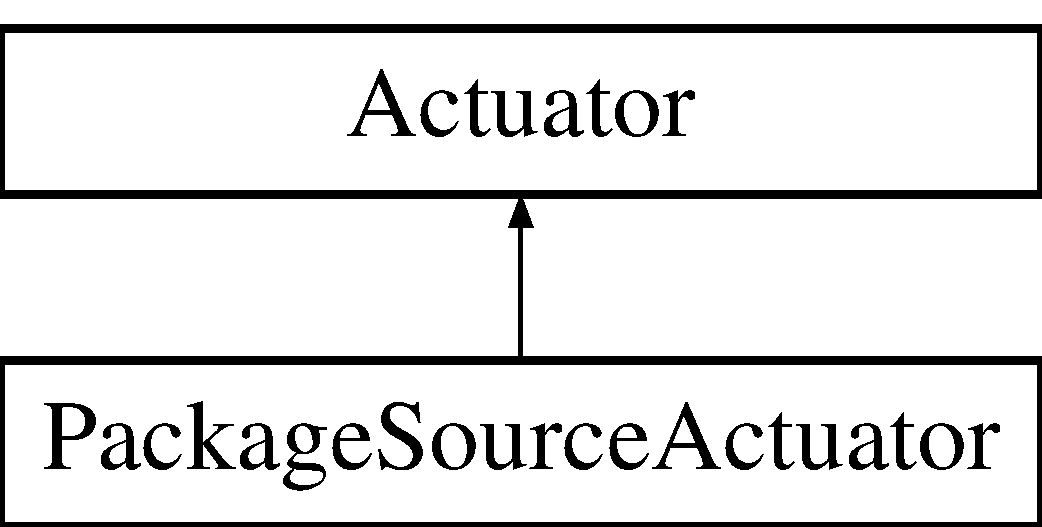
\includegraphics[height=2.000000cm]{classPackageSourceActuator}
\end{center}
\end{figure}
\subsection*{Public Member Functions}
\begin{DoxyCompactItemize}
\item 
\hyperlink{classPackageSourceActuator_a8be44f996eef9829a49d0cef77db033e}{Package\-Source\-Actuator} (int id, \hyperlink{classPackageSource}{Package\-Source} $\ast$package\-Source)
\item 
virtual void \hyperlink{classPackageSourceActuator_ab27c455d40d832ed4558f893f1ed3565}{draw\-Label} ()
\item 
void \hyperlink{classPackageSourceActuator_a67e19fb7457c9c29288d8409446756f0}{set} (signed int value)
\item 
void \hyperlink{classPackageSourceActuator_a058a225a850f0d49a79f90700ada3254}{run} ()
\end{DoxyCompactItemize}
\subsection*{Public Attributes}
\begin{DoxyCompactItemize}
\item 
\hyperlink{classPackageSource}{Package\-Source} $\ast$ \hyperlink{classPackageSourceActuator_a7104c9ab657025a7f245f92f38b27b71}{m\-\_\-package\-Source}
\end{DoxyCompactItemize}


\subsection{Detailed Description}
Produce packages at a specific position, by controlling a package-\/source. 

\subsection{Constructor \& Destructor Documentation}
\hypertarget{classPackageSourceActuator_a8be44f996eef9829a49d0cef77db033e}{\index{Package\-Source\-Actuator@{Package\-Source\-Actuator}!Package\-Source\-Actuator@{Package\-Source\-Actuator}}
\index{Package\-Source\-Actuator@{Package\-Source\-Actuator}!PackageSourceActuator@{Package\-Source\-Actuator}}
\subsubsection[{Package\-Source\-Actuator}]{\setlength{\rightskip}{0pt plus 5cm}Package\-Source\-Actuator\-::\-Package\-Source\-Actuator (
\begin{DoxyParamCaption}
\item[{int}]{id, }
\item[{{\bf Package\-Source} $\ast$}]{package\-Source}
\end{DoxyParamCaption}
)}}\label{classPackageSourceActuator_a8be44f996eef9829a49d0cef77db033e}


\subsection{Member Function Documentation}
\hypertarget{classPackageSourceActuator_ab27c455d40d832ed4558f893f1ed3565}{\index{Package\-Source\-Actuator@{Package\-Source\-Actuator}!draw\-Label@{draw\-Label}}
\index{draw\-Label@{draw\-Label}!PackageSourceActuator@{Package\-Source\-Actuator}}
\subsubsection[{draw\-Label}]{\setlength{\rightskip}{0pt plus 5cm}void Package\-Source\-Actuator\-::draw\-Label (
\begin{DoxyParamCaption}
{}
\end{DoxyParamCaption}
)\hspace{0.3cm}{\ttfamily [virtual]}}}\label{classPackageSourceActuator_ab27c455d40d832ed4558f893f1ed3565}


Reimplemented from \hyperlink{classActuator_aaa39a438315ac34dbb1a4237bf70ff99}{Actuator}.

\hypertarget{classPackageSourceActuator_a058a225a850f0d49a79f90700ada3254}{\index{Package\-Source\-Actuator@{Package\-Source\-Actuator}!run@{run}}
\index{run@{run}!PackageSourceActuator@{Package\-Source\-Actuator}}
\subsubsection[{run}]{\setlength{\rightskip}{0pt plus 5cm}void Package\-Source\-Actuator\-::run (
\begin{DoxyParamCaption}
{}
\end{DoxyParamCaption}
)\hspace{0.3cm}{\ttfamily [virtual]}}}\label{classPackageSourceActuator_a058a225a850f0d49a79f90700ada3254}


Reimplemented from \hyperlink{classActuator_aabe48a4249a91a4cd1b964001fe754fc}{Actuator}.

\hypertarget{classPackageSourceActuator_a67e19fb7457c9c29288d8409446756f0}{\index{Package\-Source\-Actuator@{Package\-Source\-Actuator}!set@{set}}
\index{set@{set}!PackageSourceActuator@{Package\-Source\-Actuator}}
\subsubsection[{set}]{\setlength{\rightskip}{0pt plus 5cm}void Package\-Source\-Actuator\-::set (
\begin{DoxyParamCaption}
\item[{signed int}]{value}
\end{DoxyParamCaption}
)\hspace{0.3cm}{\ttfamily [virtual]}}}\label{classPackageSourceActuator_a67e19fb7457c9c29288d8409446756f0}


Reimplemented from \hyperlink{classActuator_a6281019cccd4034ab2cf7071defecf70}{Actuator}.



\subsection{Member Data Documentation}
\hypertarget{classPackageSourceActuator_a7104c9ab657025a7f245f92f38b27b71}{\index{Package\-Source\-Actuator@{Package\-Source\-Actuator}!m\-\_\-package\-Source@{m\-\_\-package\-Source}}
\index{m\-\_\-package\-Source@{m\-\_\-package\-Source}!PackageSourceActuator@{Package\-Source\-Actuator}}
\subsubsection[{m\-\_\-package\-Source}]{\setlength{\rightskip}{0pt plus 5cm}{\bf Package\-Source}$\ast$ Package\-Source\-Actuator\-::m\-\_\-package\-Source}}\label{classPackageSourceActuator_a7104c9ab657025a7f245f92f38b27b71}


The documentation for this class was generated from the following files\-:\begin{DoxyCompactItemize}
\item 
\hyperlink{Actuators_8h}{Actuators.\-h}\item 
\hyperlink{Actuators_8cpp}{Actuators.\-cpp}\end{DoxyCompactItemize}

\hypertarget{classPlank}{\section{Plank Class Reference}
\label{classPlank}\index{Plank@{Plank}}
}


Represent Plank-\/objects.  




{\ttfamily \#include $<$Package.\-h$>$}

\subsection*{Public Member Functions}
\begin{DoxyCompactItemize}
\item 
\hyperlink{classPlank_ad76b1cdbf4909225eb58acaa577bcd5d}{Plank} (b2\-Vec2 pos, b2\-World $\ast$world)
\item 
\hyperlink{classPlank_a478e9bd1531adca6e8250ae11d0ed07a}{$\sim$\-Plank} ()
\item 
float \hyperlink{classPlank_a3f38a8e62a692f49cfcccf6692069ceb}{random\-Float} (float a, float b)
\begin{DoxyCompactList}\small\item\em Generate random number in interval \mbox{[}a,b\mbox{]}. \end{DoxyCompactList}\item 
float32 \hyperlink{classPlank_a2f83307bc8a6a95222a343395475dce7}{get\-Width} ()
\item 
float32 \hyperlink{classPlank_a5203208bd700934affd95cc0b7bd7234}{get\-Thickness} ()
\end{DoxyCompactItemize}
\subsection*{Private Attributes}
\begin{DoxyCompactItemize}
\item 
b2\-Body\-Def $\ast$ \hyperlink{classPlank_a2d0f77c8e5716733d9715bdd641987b4}{m\-\_\-bd}
\item 
b2\-Fixture\-Def $\ast$ \hyperlink{classPlank_ad9ee0dbf22fe79689efddda7d7a94347}{m\-\_\-fd}
\item 
b2\-World $\ast$ \hyperlink{classPlank_a13c403210d33ed7d7183cfd6dd71b494}{m\-\_\-world}
\item 
float32 \hyperlink{classPlank_a188c7ef7af7fdc72d9e4925299248677}{m\-\_\-width}
\item 
float32 \hyperlink{classPlank_aba0b2459614c6427abf50c5b16c623c3}{m\-\_\-thickness}
\item 
b2\-Body $\ast$ \hyperlink{classPlank_a311d983aad3e0cd5d5059edb37f5e1b6}{m\-\_\-body}
\end{DoxyCompactItemize}


\subsection{Detailed Description}
Represent Plank-\/objects. 

 

\subsection{Constructor \& Destructor Documentation}
\hypertarget{classPlank_ad76b1cdbf4909225eb58acaa577bcd5d}{\index{Plank@{Plank}!Plank@{Plank}}
\index{Plank@{Plank}!Plank@{Plank}}
\subsubsection[{Plank}]{\setlength{\rightskip}{0pt plus 5cm}Plank\-::\-Plank (
\begin{DoxyParamCaption}
\item[{b2\-Vec2}]{pos, }
\item[{b2\-World $\ast$}]{world}
\end{DoxyParamCaption}
)}}\label{classPlank_ad76b1cdbf4909225eb58acaa577bcd5d}

\begin{DoxyParams}{Parameters}
{\em pos} & The position at which you want place the center of the plank. \\
\hline
{\em world} & Pointer to the world in which you want to create the plank. \\
\hline
\end{DoxyParams}
\hypertarget{classPlank_a478e9bd1531adca6e8250ae11d0ed07a}{\index{Plank@{Plank}!$\sim$\-Plank@{$\sim$\-Plank}}
\index{$\sim$\-Plank@{$\sim$\-Plank}!Plank@{Plank}}
\subsubsection[{$\sim$\-Plank}]{\setlength{\rightskip}{0pt plus 5cm}Plank\-::$\sim$\-Plank (
\begin{DoxyParamCaption}
{}
\end{DoxyParamCaption}
)}}\label{classPlank_a478e9bd1531adca6e8250ae11d0ed07a}


\subsection{Member Function Documentation}
\hypertarget{classPlank_a5203208bd700934affd95cc0b7bd7234}{\index{Plank@{Plank}!get\-Thickness@{get\-Thickness}}
\index{get\-Thickness@{get\-Thickness}!Plank@{Plank}}
\subsubsection[{get\-Thickness}]{\setlength{\rightskip}{0pt plus 5cm}float32 Plank\-::get\-Thickness (
\begin{DoxyParamCaption}
{}
\end{DoxyParamCaption}
)\hspace{0.3cm}{\ttfamily [inline]}}}\label{classPlank_a5203208bd700934affd95cc0b7bd7234}
\hypertarget{classPlank_a2f83307bc8a6a95222a343395475dce7}{\index{Plank@{Plank}!get\-Width@{get\-Width}}
\index{get\-Width@{get\-Width}!Plank@{Plank}}
\subsubsection[{get\-Width}]{\setlength{\rightskip}{0pt plus 5cm}float32 Plank\-::get\-Width (
\begin{DoxyParamCaption}
{}
\end{DoxyParamCaption}
)\hspace{0.3cm}{\ttfamily [inline]}}}\label{classPlank_a2f83307bc8a6a95222a343395475dce7}
\hypertarget{classPlank_a3f38a8e62a692f49cfcccf6692069ceb}{\index{Plank@{Plank}!random\-Float@{random\-Float}}
\index{random\-Float@{random\-Float}!Plank@{Plank}}
\subsubsection[{random\-Float}]{\setlength{\rightskip}{0pt plus 5cm}float Plank\-::random\-Float (
\begin{DoxyParamCaption}
\item[{float}]{a, }
\item[{float}]{b}
\end{DoxyParamCaption}
)}}\label{classPlank_a3f38a8e62a692f49cfcccf6692069ceb}


Generate random number in interval \mbox{[}a,b\mbox{]}. 

Helper-\/function used to give planks random length and quality.


\begin{DoxyParams}{Parameters}
{\em a} & Start of interval \\
\hline
{\em b} & End of interval \\
\hline
\end{DoxyParams}
\begin{DoxyReturn}{Returns}
a random number from the interval \mbox{[}a,b\mbox{]} 
\end{DoxyReturn}


\subsection{Member Data Documentation}
\hypertarget{classPlank_a2d0f77c8e5716733d9715bdd641987b4}{\index{Plank@{Plank}!m\-\_\-bd@{m\-\_\-bd}}
\index{m\-\_\-bd@{m\-\_\-bd}!Plank@{Plank}}
\subsubsection[{m\-\_\-bd}]{\setlength{\rightskip}{0pt plus 5cm}b2\-Body\-Def$\ast$ Plank\-::m\-\_\-bd\hspace{0.3cm}{\ttfamily [private]}}}\label{classPlank_a2d0f77c8e5716733d9715bdd641987b4}
\hypertarget{classPlank_a311d983aad3e0cd5d5059edb37f5e1b6}{\index{Plank@{Plank}!m\-\_\-body@{m\-\_\-body}}
\index{m\-\_\-body@{m\-\_\-body}!Plank@{Plank}}
\subsubsection[{m\-\_\-body}]{\setlength{\rightskip}{0pt plus 5cm}b2\-Body$\ast$ Plank\-::m\-\_\-body\hspace{0.3cm}{\ttfamily [private]}}}\label{classPlank_a311d983aad3e0cd5d5059edb37f5e1b6}
\hypertarget{classPlank_ad9ee0dbf22fe79689efddda7d7a94347}{\index{Plank@{Plank}!m\-\_\-fd@{m\-\_\-fd}}
\index{m\-\_\-fd@{m\-\_\-fd}!Plank@{Plank}}
\subsubsection[{m\-\_\-fd}]{\setlength{\rightskip}{0pt plus 5cm}b2\-Fixture\-Def$\ast$ Plank\-::m\-\_\-fd\hspace{0.3cm}{\ttfamily [private]}}}\label{classPlank_ad9ee0dbf22fe79689efddda7d7a94347}
\hypertarget{classPlank_aba0b2459614c6427abf50c5b16c623c3}{\index{Plank@{Plank}!m\-\_\-thickness@{m\-\_\-thickness}}
\index{m\-\_\-thickness@{m\-\_\-thickness}!Plank@{Plank}}
\subsubsection[{m\-\_\-thickness}]{\setlength{\rightskip}{0pt plus 5cm}float32 Plank\-::m\-\_\-thickness\hspace{0.3cm}{\ttfamily [private]}}}\label{classPlank_aba0b2459614c6427abf50c5b16c623c3}
\hypertarget{classPlank_a188c7ef7af7fdc72d9e4925299248677}{\index{Plank@{Plank}!m\-\_\-width@{m\-\_\-width}}
\index{m\-\_\-width@{m\-\_\-width}!Plank@{Plank}}
\subsubsection[{m\-\_\-width}]{\setlength{\rightskip}{0pt plus 5cm}float32 Plank\-::m\-\_\-width\hspace{0.3cm}{\ttfamily [private]}}}\label{classPlank_a188c7ef7af7fdc72d9e4925299248677}
\hypertarget{classPlank_a13c403210d33ed7d7183cfd6dd71b494}{\index{Plank@{Plank}!m\-\_\-world@{m\-\_\-world}}
\index{m\-\_\-world@{m\-\_\-world}!Plank@{Plank}}
\subsubsection[{m\-\_\-world}]{\setlength{\rightskip}{0pt plus 5cm}b2\-World$\ast$ Plank\-::m\-\_\-world\hspace{0.3cm}{\ttfamily [private]}}}\label{classPlank_a13c403210d33ed7d7183cfd6dd71b494}


The documentation for this class was generated from the following files\-:\begin{DoxyCompactItemize}
\item 
\hyperlink{Package_8h}{Package.\-h}\item 
\hyperlink{Package_8cpp}{Package.\-cpp}\end{DoxyCompactItemize}

\hypertarget{classPlankSortingPlant}{\section{Plank\-Sorting\-Plant Class Reference}
\label{classPlankSortingPlant}\index{Plank\-Sorting\-Plant@{Plank\-Sorting\-Plant}}
}


Extend the default \hyperlink{classSimulatorPage}{Simulator\-Page} to create a simulation of a plank sorting plant.  




{\ttfamily \#include $<$Plank\-Sorting\-Plant.\-h$>$}

Inheritance diagram for Plank\-Sorting\-Plant\-:\begin{figure}[H]
\begin{center}
\leavevmode
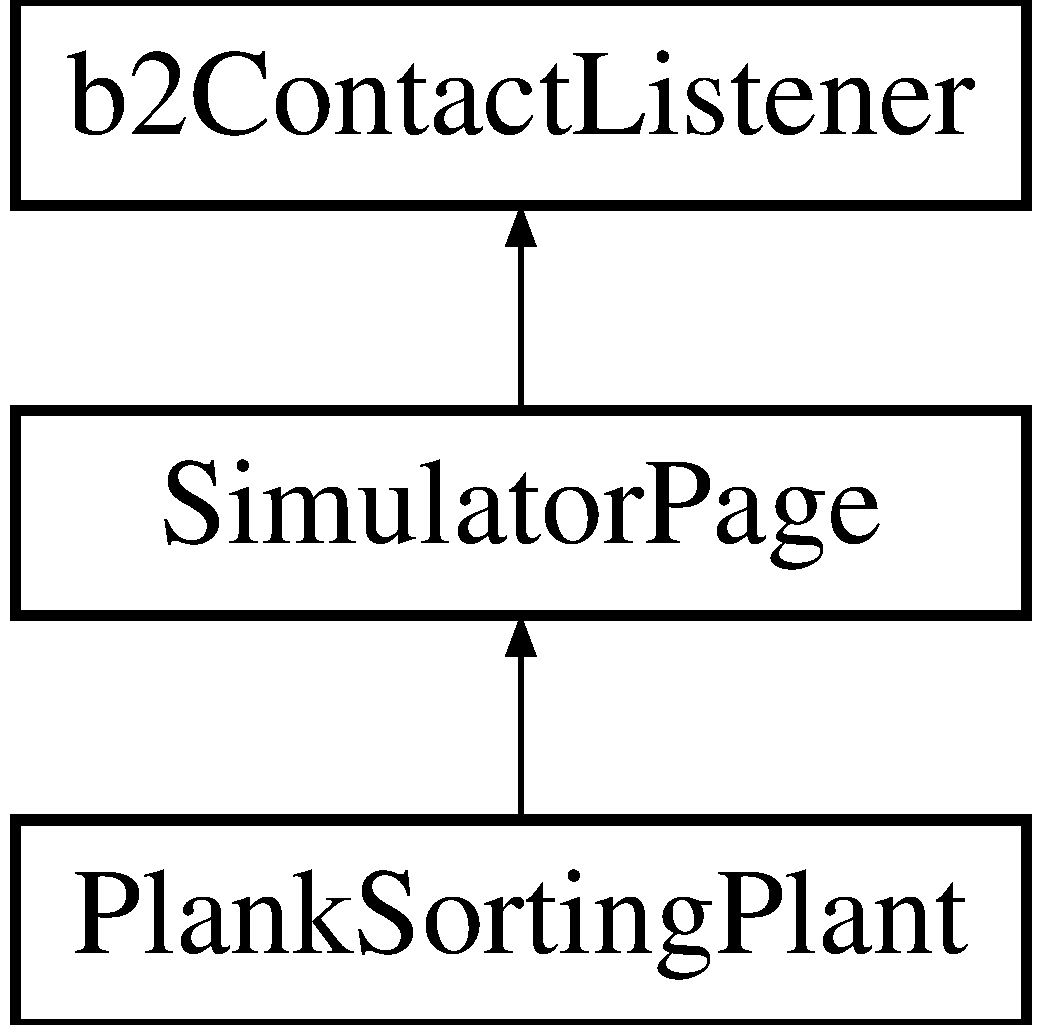
\includegraphics[height=3.000000cm]{classPlankSortingPlant}
\end{center}
\end{figure}
\subsection*{Public Member Functions}
\begin{DoxyCompactItemize}
\item 
\hyperlink{classPlankSortingPlant_a1cb45c8ff425d982f421b8226d0ce578}{Plank\-Sorting\-Plant} (\hyperlink{classCommunicator}{Communicator} $\ast$communicator)
\item 
void \hyperlink{classPlankSortingPlant_a512555c258c6e6d824356af6ed2e77f2}{Step} (\hyperlink{structSettings}{Settings} $\ast$settings)
\item 
void \hyperlink{classPlankSortingPlant_a131fade1b547a3af4f2b5158bc285e30}{Keyboard} (unsigned char key)
\end{DoxyCompactItemize}
\subsection*{Static Public Member Functions}
\begin{DoxyCompactItemize}
\item 
static \hyperlink{classSimulatorPage}{Simulator\-Page} $\ast$ \hyperlink{classPlankSortingPlant_ad576fadff9a31216c061cabce2071cf8}{Create} (\hyperlink{classCommunicator}{Communicator} $\ast$communicator)
\end{DoxyCompactItemize}
\subsection*{Private Attributes}
\begin{DoxyCompactItemize}
\item 
\hyperlink{classConveyor}{Conveyor} $\ast$ \hyperlink{classPlankSortingPlant_ad5ba935847d141b8dc9842e369b8fa75}{m\-\_\-conveyor1}
\item 
\hyperlink{classConveyor}{Conveyor} $\ast$ \hyperlink{classPlankSortingPlant_a97274155c82f74a78cf12b85bb21ef1a}{m\-\_\-conveyor2}
\item 
\hyperlink{classConveyor}{Conveyor} $\ast$ \hyperlink{classPlankSortingPlant_a371d083cde882e616fa2662ba8c54697}{m\-\_\-conveyor3}
\item 
\hyperlink{classConveyor}{Conveyor} $\ast$ \hyperlink{classPlankSortingPlant_a3bc33fc093ed704b987e2ae109aa5272}{m\-\_\-conveyor4}
\item 
\hyperlink{classConveyor}{Conveyor} $\ast$ \hyperlink{classPlankSortingPlant_ac4b0efb2fee3b1b0b15637577de11533}{m\-\_\-conveyor5}
\item 
\hyperlink{classConveyor}{Conveyor} $\ast$ \hyperlink{classPlankSortingPlant_a2996b20c8f489aa477f9f795b15f1763}{m\-\_\-conveyor6}
\item 
\hyperlink{classConveyor}{Conveyor} $\ast$ \hyperlink{classPlankSortingPlant_a34e6abc7cc90688e30ed11496c535d7f}{m\-\_\-conveyor7}
\item 
\hyperlink{classConveyor}{Conveyor} $\ast$ \hyperlink{classPlankSortingPlant_aa0f88ed0f453772b867ad77adfeb2c16}{m\-\_\-conveyor8}
\item 
\hyperlink{classWheel}{Wheel} $\ast$ \hyperlink{classPlankSortingPlant_a755d0e2c79ee575d469f2db9011cf4f1}{m\-\_\-wheel1}
\item 
\hyperlink{classWheel}{Wheel} $\ast$ \hyperlink{classPlankSortingPlant_a60a0596b799edbeef6d8a61a1e6bd9fc}{m\-\_\-wheel2}
\item 
\hyperlink{classConveyorSynchronizer}{Conveyor\-Synchronizer} $\ast$ \hyperlink{classPlankSortingPlant_a944ee04de6f8ba2afa71474061fac329}{m\-\_\-conveyor\-Synchronizer}
\item 
\hyperlink{classCommandSequenceInterpreter}{Command\-Sequence\-Interpreter} $\ast$ \hyperlink{classPlankSortingPlant_ab4428fbbce9a7023848de19be0525156}{m\-\_\-command\-Sequence\-Interpreter}
\item 
\hyperlink{classActuatorSet}{Actuator\-Set} $\ast$ \hyperlink{classPlankSortingPlant_ab6c83de131a92e26c4b007a64d84dcfe}{m\-\_\-actuator\-Set}
\item 
\hyperlink{classSensorSet}{Sensor\-Set} $\ast$ \hyperlink{classPlankSortingPlant_a4946e0e57ac1049bb7602708f884579b}{m\-\_\-sensor\-Set}
\end{DoxyCompactItemize}
\subsection*{Additional Inherited Members}


\subsection{Detailed Description}
Extend the default \hyperlink{classSimulatorPage}{Simulator\-Page} to create a simulation of a plank sorting plant. 

A snapshot of the plant\-: 

You are welcome to add your own Simulator\-Pages in the file \hyperlink{SimulatorPageEntries_8cpp}{Simulator\-Page\-Entries.\-cpp} in this maner\-: 
\begin{DoxyCode}
\hyperlink{structSimulatorPageEntry}{SimulatorPageEntry} g\_simulatorPageEntries[] =
\{
    \{\textcolor{stringliteral}{"Plank sorting plant"}, \hyperlink{classPlankSortingPlant_ad576fadff9a31216c061cabce2071cf8}{PlankSortingPlant::Create}\}
      ,
    \{NULL, NULL\}
\}
\end{DoxyCode}
 

\subsection{Constructor \& Destructor Documentation}
\hypertarget{classPlankSortingPlant_a1cb45c8ff425d982f421b8226d0ce578}{\index{Plank\-Sorting\-Plant@{Plank\-Sorting\-Plant}!Plank\-Sorting\-Plant@{Plank\-Sorting\-Plant}}
\index{Plank\-Sorting\-Plant@{Plank\-Sorting\-Plant}!PlankSortingPlant@{Plank\-Sorting\-Plant}}
\subsubsection[{Plank\-Sorting\-Plant}]{\setlength{\rightskip}{0pt plus 5cm}Plank\-Sorting\-Plant\-::\-Plank\-Sorting\-Plant (
\begin{DoxyParamCaption}
\item[{{\bf Communicator} $\ast$}]{communicator}
\end{DoxyParamCaption}
)}}\label{classPlankSortingPlant_a1cb45c8ff425d982f421b8226d0ce578}


\subsection{Member Function Documentation}
\hypertarget{classPlankSortingPlant_ad576fadff9a31216c061cabce2071cf8}{\index{Plank\-Sorting\-Plant@{Plank\-Sorting\-Plant}!Create@{Create}}
\index{Create@{Create}!PlankSortingPlant@{Plank\-Sorting\-Plant}}
\subsubsection[{Create}]{\setlength{\rightskip}{0pt plus 5cm}{\bf Simulator\-Page} $\ast$ Plank\-Sorting\-Plant\-::\-Create (
\begin{DoxyParamCaption}
\item[{{\bf Communicator} $\ast$}]{communicator}
\end{DoxyParamCaption}
)\hspace{0.3cm}{\ttfamily [static]}}}\label{classPlankSortingPlant_ad576fadff9a31216c061cabce2071cf8}
\hypertarget{classPlankSortingPlant_a131fade1b547a3af4f2b5158bc285e30}{\index{Plank\-Sorting\-Plant@{Plank\-Sorting\-Plant}!Keyboard@{Keyboard}}
\index{Keyboard@{Keyboard}!PlankSortingPlant@{Plank\-Sorting\-Plant}}
\subsubsection[{Keyboard}]{\setlength{\rightskip}{0pt plus 5cm}void Plank\-Sorting\-Plant\-::\-Keyboard (
\begin{DoxyParamCaption}
\item[{unsigned char}]{key}
\end{DoxyParamCaption}
)\hspace{0.3cm}{\ttfamily [virtual]}}}\label{classPlankSortingPlant_a131fade1b547a3af4f2b5158bc285e30}


Reimplemented from \hyperlink{classSimulatorPage_a295bcbd72dfe0dd651d922b8165e8f9a}{Simulator\-Page}.

\hypertarget{classPlankSortingPlant_a512555c258c6e6d824356af6ed2e77f2}{\index{Plank\-Sorting\-Plant@{Plank\-Sorting\-Plant}!Step@{Step}}
\index{Step@{Step}!PlankSortingPlant@{Plank\-Sorting\-Plant}}
\subsubsection[{Step}]{\setlength{\rightskip}{0pt plus 5cm}void Plank\-Sorting\-Plant\-::\-Step (
\begin{DoxyParamCaption}
\item[{{\bf Settings} $\ast$}]{settings}
\end{DoxyParamCaption}
)\hspace{0.3cm}{\ttfamily [virtual]}}}\label{classPlankSortingPlant_a512555c258c6e6d824356af6ed2e77f2}


Reimplemented from \hyperlink{classSimulatorPage_ac478dc8792d0f593c6dc6277a4e96719}{Simulator\-Page}.



\subsection{Member Data Documentation}
\hypertarget{classPlankSortingPlant_ab6c83de131a92e26c4b007a64d84dcfe}{\index{Plank\-Sorting\-Plant@{Plank\-Sorting\-Plant}!m\-\_\-actuator\-Set@{m\-\_\-actuator\-Set}}
\index{m\-\_\-actuator\-Set@{m\-\_\-actuator\-Set}!PlankSortingPlant@{Plank\-Sorting\-Plant}}
\subsubsection[{m\-\_\-actuator\-Set}]{\setlength{\rightskip}{0pt plus 5cm}{\bf Actuator\-Set}$\ast$ Plank\-Sorting\-Plant\-::m\-\_\-actuator\-Set\hspace{0.3cm}{\ttfamily [private]}}}\label{classPlankSortingPlant_ab6c83de131a92e26c4b007a64d84dcfe}
\hypertarget{classPlankSortingPlant_ab4428fbbce9a7023848de19be0525156}{\index{Plank\-Sorting\-Plant@{Plank\-Sorting\-Plant}!m\-\_\-command\-Sequence\-Interpreter@{m\-\_\-command\-Sequence\-Interpreter}}
\index{m\-\_\-command\-Sequence\-Interpreter@{m\-\_\-command\-Sequence\-Interpreter}!PlankSortingPlant@{Plank\-Sorting\-Plant}}
\subsubsection[{m\-\_\-command\-Sequence\-Interpreter}]{\setlength{\rightskip}{0pt plus 5cm}{\bf Command\-Sequence\-Interpreter}$\ast$ Plank\-Sorting\-Plant\-::m\-\_\-command\-Sequence\-Interpreter\hspace{0.3cm}{\ttfamily [private]}}}\label{classPlankSortingPlant_ab4428fbbce9a7023848de19be0525156}
\hypertarget{classPlankSortingPlant_ad5ba935847d141b8dc9842e369b8fa75}{\index{Plank\-Sorting\-Plant@{Plank\-Sorting\-Plant}!m\-\_\-conveyor1@{m\-\_\-conveyor1}}
\index{m\-\_\-conveyor1@{m\-\_\-conveyor1}!PlankSortingPlant@{Plank\-Sorting\-Plant}}
\subsubsection[{m\-\_\-conveyor1}]{\setlength{\rightskip}{0pt plus 5cm}{\bf Conveyor}$\ast$ Plank\-Sorting\-Plant\-::m\-\_\-conveyor1\hspace{0.3cm}{\ttfamily [private]}}}\label{classPlankSortingPlant_ad5ba935847d141b8dc9842e369b8fa75}
\hypertarget{classPlankSortingPlant_a97274155c82f74a78cf12b85bb21ef1a}{\index{Plank\-Sorting\-Plant@{Plank\-Sorting\-Plant}!m\-\_\-conveyor2@{m\-\_\-conveyor2}}
\index{m\-\_\-conveyor2@{m\-\_\-conveyor2}!PlankSortingPlant@{Plank\-Sorting\-Plant}}
\subsubsection[{m\-\_\-conveyor2}]{\setlength{\rightskip}{0pt plus 5cm}{\bf Conveyor}$\ast$ Plank\-Sorting\-Plant\-::m\-\_\-conveyor2\hspace{0.3cm}{\ttfamily [private]}}}\label{classPlankSortingPlant_a97274155c82f74a78cf12b85bb21ef1a}
\hypertarget{classPlankSortingPlant_a371d083cde882e616fa2662ba8c54697}{\index{Plank\-Sorting\-Plant@{Plank\-Sorting\-Plant}!m\-\_\-conveyor3@{m\-\_\-conveyor3}}
\index{m\-\_\-conveyor3@{m\-\_\-conveyor3}!PlankSortingPlant@{Plank\-Sorting\-Plant}}
\subsubsection[{m\-\_\-conveyor3}]{\setlength{\rightskip}{0pt plus 5cm}{\bf Conveyor}$\ast$ Plank\-Sorting\-Plant\-::m\-\_\-conveyor3\hspace{0.3cm}{\ttfamily [private]}}}\label{classPlankSortingPlant_a371d083cde882e616fa2662ba8c54697}
\hypertarget{classPlankSortingPlant_a3bc33fc093ed704b987e2ae109aa5272}{\index{Plank\-Sorting\-Plant@{Plank\-Sorting\-Plant}!m\-\_\-conveyor4@{m\-\_\-conveyor4}}
\index{m\-\_\-conveyor4@{m\-\_\-conveyor4}!PlankSortingPlant@{Plank\-Sorting\-Plant}}
\subsubsection[{m\-\_\-conveyor4}]{\setlength{\rightskip}{0pt plus 5cm}{\bf Conveyor}$\ast$ Plank\-Sorting\-Plant\-::m\-\_\-conveyor4\hspace{0.3cm}{\ttfamily [private]}}}\label{classPlankSortingPlant_a3bc33fc093ed704b987e2ae109aa5272}
\hypertarget{classPlankSortingPlant_ac4b0efb2fee3b1b0b15637577de11533}{\index{Plank\-Sorting\-Plant@{Plank\-Sorting\-Plant}!m\-\_\-conveyor5@{m\-\_\-conveyor5}}
\index{m\-\_\-conveyor5@{m\-\_\-conveyor5}!PlankSortingPlant@{Plank\-Sorting\-Plant}}
\subsubsection[{m\-\_\-conveyor5}]{\setlength{\rightskip}{0pt plus 5cm}{\bf Conveyor}$\ast$ Plank\-Sorting\-Plant\-::m\-\_\-conveyor5\hspace{0.3cm}{\ttfamily [private]}}}\label{classPlankSortingPlant_ac4b0efb2fee3b1b0b15637577de11533}
\hypertarget{classPlankSortingPlant_a2996b20c8f489aa477f9f795b15f1763}{\index{Plank\-Sorting\-Plant@{Plank\-Sorting\-Plant}!m\-\_\-conveyor6@{m\-\_\-conveyor6}}
\index{m\-\_\-conveyor6@{m\-\_\-conveyor6}!PlankSortingPlant@{Plank\-Sorting\-Plant}}
\subsubsection[{m\-\_\-conveyor6}]{\setlength{\rightskip}{0pt plus 5cm}{\bf Conveyor}$\ast$ Plank\-Sorting\-Plant\-::m\-\_\-conveyor6\hspace{0.3cm}{\ttfamily [private]}}}\label{classPlankSortingPlant_a2996b20c8f489aa477f9f795b15f1763}
\hypertarget{classPlankSortingPlant_a34e6abc7cc90688e30ed11496c535d7f}{\index{Plank\-Sorting\-Plant@{Plank\-Sorting\-Plant}!m\-\_\-conveyor7@{m\-\_\-conveyor7}}
\index{m\-\_\-conveyor7@{m\-\_\-conveyor7}!PlankSortingPlant@{Plank\-Sorting\-Plant}}
\subsubsection[{m\-\_\-conveyor7}]{\setlength{\rightskip}{0pt plus 5cm}{\bf Conveyor}$\ast$ Plank\-Sorting\-Plant\-::m\-\_\-conveyor7\hspace{0.3cm}{\ttfamily [private]}}}\label{classPlankSortingPlant_a34e6abc7cc90688e30ed11496c535d7f}
\hypertarget{classPlankSortingPlant_aa0f88ed0f453772b867ad77adfeb2c16}{\index{Plank\-Sorting\-Plant@{Plank\-Sorting\-Plant}!m\-\_\-conveyor8@{m\-\_\-conveyor8}}
\index{m\-\_\-conveyor8@{m\-\_\-conveyor8}!PlankSortingPlant@{Plank\-Sorting\-Plant}}
\subsubsection[{m\-\_\-conveyor8}]{\setlength{\rightskip}{0pt plus 5cm}{\bf Conveyor}$\ast$ Plank\-Sorting\-Plant\-::m\-\_\-conveyor8\hspace{0.3cm}{\ttfamily [private]}}}\label{classPlankSortingPlant_aa0f88ed0f453772b867ad77adfeb2c16}
\hypertarget{classPlankSortingPlant_a944ee04de6f8ba2afa71474061fac329}{\index{Plank\-Sorting\-Plant@{Plank\-Sorting\-Plant}!m\-\_\-conveyor\-Synchronizer@{m\-\_\-conveyor\-Synchronizer}}
\index{m\-\_\-conveyor\-Synchronizer@{m\-\_\-conveyor\-Synchronizer}!PlankSortingPlant@{Plank\-Sorting\-Plant}}
\subsubsection[{m\-\_\-conveyor\-Synchronizer}]{\setlength{\rightskip}{0pt plus 5cm}{\bf Conveyor\-Synchronizer}$\ast$ Plank\-Sorting\-Plant\-::m\-\_\-conveyor\-Synchronizer\hspace{0.3cm}{\ttfamily [private]}}}\label{classPlankSortingPlant_a944ee04de6f8ba2afa71474061fac329}
\hypertarget{classPlankSortingPlant_a4946e0e57ac1049bb7602708f884579b}{\index{Plank\-Sorting\-Plant@{Plank\-Sorting\-Plant}!m\-\_\-sensor\-Set@{m\-\_\-sensor\-Set}}
\index{m\-\_\-sensor\-Set@{m\-\_\-sensor\-Set}!PlankSortingPlant@{Plank\-Sorting\-Plant}}
\subsubsection[{m\-\_\-sensor\-Set}]{\setlength{\rightskip}{0pt plus 5cm}{\bf Sensor\-Set}$\ast$ Plank\-Sorting\-Plant\-::m\-\_\-sensor\-Set\hspace{0.3cm}{\ttfamily [private]}}}\label{classPlankSortingPlant_a4946e0e57ac1049bb7602708f884579b}
\hypertarget{classPlankSortingPlant_a755d0e2c79ee575d469f2db9011cf4f1}{\index{Plank\-Sorting\-Plant@{Plank\-Sorting\-Plant}!m\-\_\-wheel1@{m\-\_\-wheel1}}
\index{m\-\_\-wheel1@{m\-\_\-wheel1}!PlankSortingPlant@{Plank\-Sorting\-Plant}}
\subsubsection[{m\-\_\-wheel1}]{\setlength{\rightskip}{0pt plus 5cm}{\bf Wheel}$\ast$ Plank\-Sorting\-Plant\-::m\-\_\-wheel1\hspace{0.3cm}{\ttfamily [private]}}}\label{classPlankSortingPlant_a755d0e2c79ee575d469f2db9011cf4f1}
\hypertarget{classPlankSortingPlant_a60a0596b799edbeef6d8a61a1e6bd9fc}{\index{Plank\-Sorting\-Plant@{Plank\-Sorting\-Plant}!m\-\_\-wheel2@{m\-\_\-wheel2}}
\index{m\-\_\-wheel2@{m\-\_\-wheel2}!PlankSortingPlant@{Plank\-Sorting\-Plant}}
\subsubsection[{m\-\_\-wheel2}]{\setlength{\rightskip}{0pt plus 5cm}{\bf Wheel}$\ast$ Plank\-Sorting\-Plant\-::m\-\_\-wheel2\hspace{0.3cm}{\ttfamily [private]}}}\label{classPlankSortingPlant_a60a0596b799edbeef6d8a61a1e6bd9fc}


The documentation for this class was generated from the following files\-:\begin{DoxyCompactItemize}
\item 
\hyperlink{PlankSortingPlant_8h}{Plank\-Sorting\-Plant.\-h}\item 
\hyperlink{PlankSortingPlant_8cpp}{Plank\-Sorting\-Plant.\-cpp}\end{DoxyCompactItemize}

\hypertarget{classPlankUserData}{\section{Plank\-User\-Data Class Reference}
\label{classPlankUserData}\index{Plank\-User\-Data@{Plank\-User\-Data}}
}


Carry information about planks.  




{\ttfamily \#include $<$User\-Data.\-h$>$}

Inheritance diagram for Plank\-User\-Data\-:\begin{figure}[H]
\begin{center}
\leavevmode
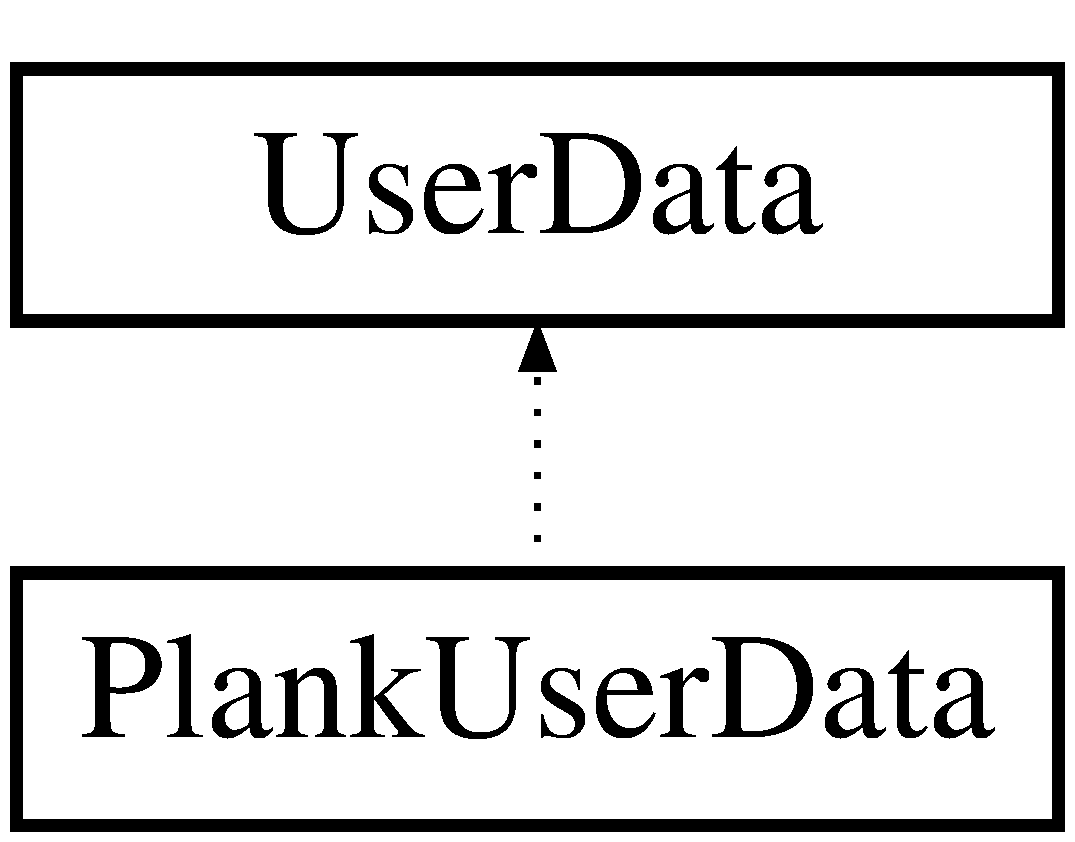
\includegraphics[height=2.000000cm]{classPlankUserData}
\end{center}
\end{figure}
\subsection*{Public Member Functions}
\begin{DoxyCompactItemize}
\item 
\hyperlink{classPlankUserData_a0357a6e184cee3a636a373095cde606d}{Plank\-User\-Data} (float32 length, float32 quality)
\end{DoxyCompactItemize}
\subsection*{Public Attributes}
\begin{DoxyCompactItemize}
\item 
float32 \hyperlink{classPlankUserData_acb52b3118340b50102503b34e102b90b}{m\-\_\-length}
\item 
float32 \hyperlink{classPlankUserData_ae4136eaef48871ffbec502cdd4660d81}{m\-\_\-quality}
\end{DoxyCompactItemize}
\subsection*{Additional Inherited Members}


\subsection{Detailed Description}
Carry information about planks. 

Each planks b2\-Fixture points to an instance of this class. Contains information about a planks objective length and planks objective quality. 

\subsection{Constructor \& Destructor Documentation}
\hypertarget{classPlankUserData_a0357a6e184cee3a636a373095cde606d}{\index{Plank\-User\-Data@{Plank\-User\-Data}!Plank\-User\-Data@{Plank\-User\-Data}}
\index{Plank\-User\-Data@{Plank\-User\-Data}!PlankUserData@{Plank\-User\-Data}}
\subsubsection[{Plank\-User\-Data}]{\setlength{\rightskip}{0pt plus 5cm}Plank\-User\-Data\-::\-Plank\-User\-Data (
\begin{DoxyParamCaption}
\item[{float32}]{length, }
\item[{float32}]{quality}
\end{DoxyParamCaption}
)\hspace{0.3cm}{\ttfamily [inline]}}}\label{classPlankUserData_a0357a6e184cee3a636a373095cde606d}


\subsection{Member Data Documentation}
\hypertarget{classPlankUserData_acb52b3118340b50102503b34e102b90b}{\index{Plank\-User\-Data@{Plank\-User\-Data}!m\-\_\-length@{m\-\_\-length}}
\index{m\-\_\-length@{m\-\_\-length}!PlankUserData@{Plank\-User\-Data}}
\subsubsection[{m\-\_\-length}]{\setlength{\rightskip}{0pt plus 5cm}float32 Plank\-User\-Data\-::m\-\_\-length}}\label{classPlankUserData_acb52b3118340b50102503b34e102b90b}
\hypertarget{classPlankUserData_ae4136eaef48871ffbec502cdd4660d81}{\index{Plank\-User\-Data@{Plank\-User\-Data}!m\-\_\-quality@{m\-\_\-quality}}
\index{m\-\_\-quality@{m\-\_\-quality}!PlankUserData@{Plank\-User\-Data}}
\subsubsection[{m\-\_\-quality}]{\setlength{\rightskip}{0pt plus 5cm}float32 Plank\-User\-Data\-::m\-\_\-quality}}\label{classPlankUserData_ae4136eaef48871ffbec502cdd4660d81}


The documentation for this class was generated from the following file\-:\begin{DoxyCompactItemize}
\item 
\hyperlink{UserData_8h}{User\-Data.\-h}\end{DoxyCompactItemize}

\hypertarget{classQualitySensor}{\section{Quality\-Sensor Class Reference}
\label{classQualitySensor}\index{Quality\-Sensor@{Quality\-Sensor}}
}


Measure quality of a colliding Plank-\/instance.  




{\ttfamily \#include $<$Sensors.\-h$>$}

Inheritance diagram for Quality\-Sensor\-:\begin{figure}[H]
\begin{center}
\leavevmode
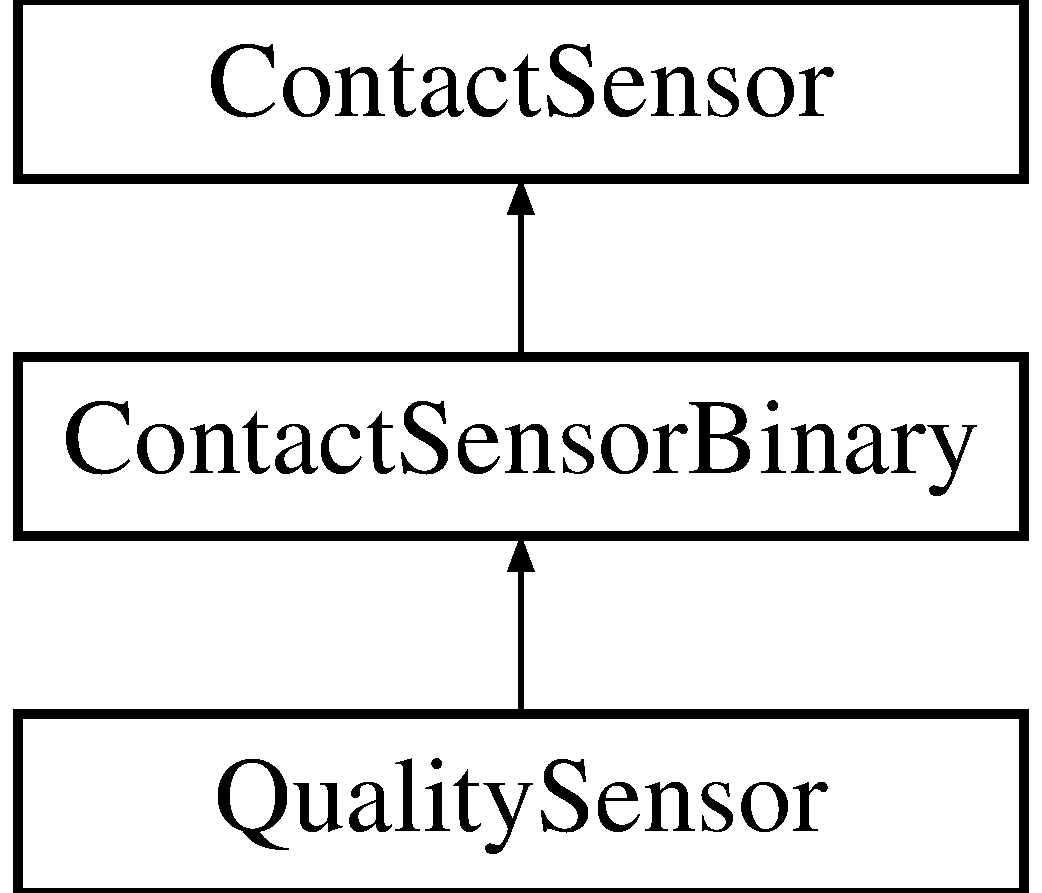
\includegraphics[height=3.000000cm]{classQualitySensor}
\end{center}
\end{figure}
\subsection*{Public Member Functions}
\begin{DoxyCompactItemize}
\item 
\hyperlink{classQualitySensor_a4ef03471dc36c3645e818b18da8a735c}{Quality\-Sensor} (int id, b2\-Vec2 position, float32 radius, b2\-World $\ast$world)
\item 
void \hyperlink{classQualitySensor_a65cff94293bca6403c88f64a1986eb53}{meassure\-Quality} (float32 quality)
\item 
signed int \hyperlink{classQualitySensor_ab8740e275a34b860b0b370183eb4d578}{get} ()
\begin{DoxyCompactList}\small\item\em Return the state of the sensor. \end{DoxyCompactList}\end{DoxyCompactItemize}
\subsection*{Public Attributes}
\begin{DoxyCompactItemize}
\item 
signed int \hyperlink{classQualitySensor_ab8ff0417a223b169e73312f06c044cde}{m\-\_\-meassured\-Quality}
\begin{DoxyCompactList}\small\item\em Store the last measured plank quality. \end{DoxyCompactList}\end{DoxyCompactItemize}


\subsection{Detailed Description}
Measure quality of a colliding Plank-\/instance. 

\subsection{Constructor \& Destructor Documentation}
\hypertarget{classQualitySensor_a4ef03471dc36c3645e818b18da8a735c}{\index{Quality\-Sensor@{Quality\-Sensor}!Quality\-Sensor@{Quality\-Sensor}}
\index{Quality\-Sensor@{Quality\-Sensor}!QualitySensor@{Quality\-Sensor}}
\subsubsection[{Quality\-Sensor}]{\setlength{\rightskip}{0pt plus 5cm}Quality\-Sensor\-::\-Quality\-Sensor (
\begin{DoxyParamCaption}
\item[{int}]{id, }
\item[{b2\-Vec2}]{position, }
\item[{float32}]{radius, }
\item[{b2\-World $\ast$}]{world}
\end{DoxyParamCaption}
)}}\label{classQualitySensor_a4ef03471dc36c3645e818b18da8a735c}


\subsection{Member Function Documentation}
\hypertarget{classQualitySensor_ab8740e275a34b860b0b370183eb4d578}{\index{Quality\-Sensor@{Quality\-Sensor}!get@{get}}
\index{get@{get}!QualitySensor@{Quality\-Sensor}}
\subsubsection[{get}]{\setlength{\rightskip}{0pt plus 5cm}signed int Quality\-Sensor\-::get (
\begin{DoxyParamCaption}
{}
\end{DoxyParamCaption}
)\hspace{0.3cm}{\ttfamily [inline]}, {\ttfamily [virtual]}}}\label{classQualitySensor_ab8740e275a34b860b0b370183eb4d578}


Return the state of the sensor. 



Reimplemented from \hyperlink{classContactSensorBinary_a68e856e0d580f91f518099874f8c226b}{Contact\-Sensor\-Binary}.

\hypertarget{classQualitySensor_a65cff94293bca6403c88f64a1986eb53}{\index{Quality\-Sensor@{Quality\-Sensor}!meassure\-Quality@{meassure\-Quality}}
\index{meassure\-Quality@{meassure\-Quality}!QualitySensor@{Quality\-Sensor}}
\subsubsection[{meassure\-Quality}]{\setlength{\rightskip}{0pt plus 5cm}void Quality\-Sensor\-::meassure\-Quality (
\begin{DoxyParamCaption}
\item[{float32}]{quality}
\end{DoxyParamCaption}
)}}\label{classQualitySensor_a65cff94293bca6403c88f64a1986eb53}


\subsection{Member Data Documentation}
\hypertarget{classQualitySensor_ab8ff0417a223b169e73312f06c044cde}{\index{Quality\-Sensor@{Quality\-Sensor}!m\-\_\-meassured\-Quality@{m\-\_\-meassured\-Quality}}
\index{m\-\_\-meassured\-Quality@{m\-\_\-meassured\-Quality}!QualitySensor@{Quality\-Sensor}}
\subsubsection[{m\-\_\-meassured\-Quality}]{\setlength{\rightskip}{0pt plus 5cm}signed int Quality\-Sensor\-::m\-\_\-meassured\-Quality}}\label{classQualitySensor_ab8ff0417a223b169e73312f06c044cde}


Store the last measured plank quality. 



The documentation for this class was generated from the following files\-:\begin{DoxyCompactItemize}
\item 
\hyperlink{Sensors_8h}{Sensors.\-h}\item 
\hyperlink{Sensors_8cpp}{Sensors.\-cpp}\end{DoxyCompactItemize}

\hypertarget{classQueryCallback}{\section{Query\-Callback Class Reference}
\label{classQueryCallback}\index{Query\-Callback@{Query\-Callback}}
}
Inheritance diagram for Query\-Callback\-:\begin{figure}[H]
\begin{center}
\leavevmode
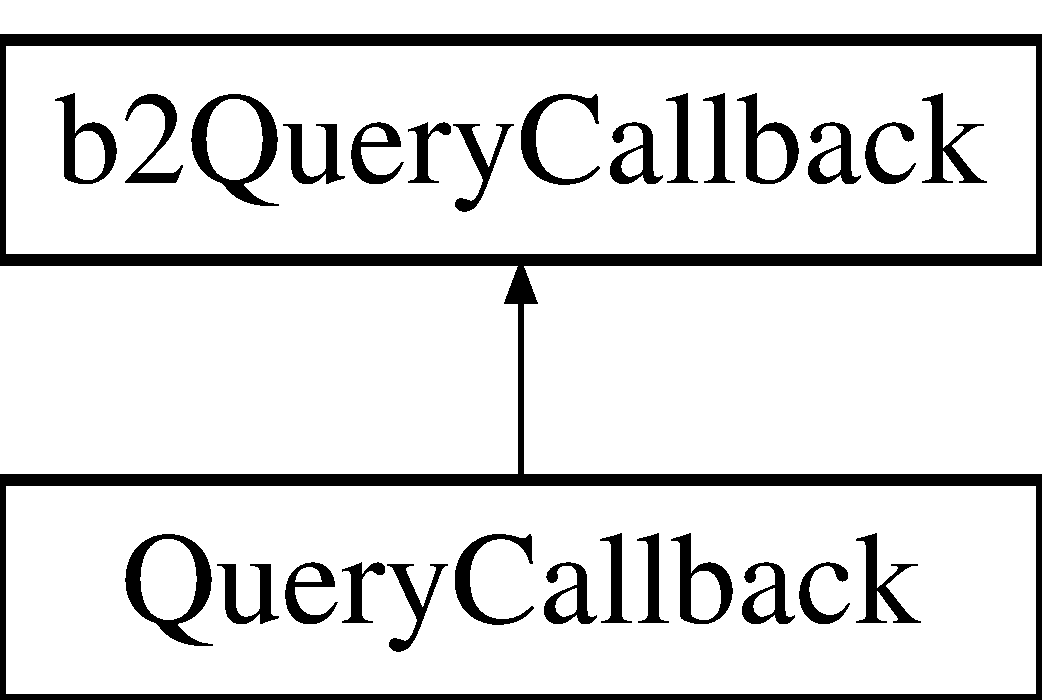
\includegraphics[height=2.000000cm]{classQueryCallback}
\end{center}
\end{figure}
\subsection*{Public Member Functions}
\begin{DoxyCompactItemize}
\item 
\hyperlink{classQueryCallback_a9c15d04aa8895b319f93e6c9af1c59f6}{Query\-Callback} (const b2\-Vec2 \&point)
\item 
bool \hyperlink{classQueryCallback_ac79cf9e2008bdea68ab3d9d64811dc62}{Report\-Fixture} (b2\-Fixture $\ast$fixture)
\end{DoxyCompactItemize}
\subsection*{Public Attributes}
\begin{DoxyCompactItemize}
\item 
b2\-Vec2 \hyperlink{classQueryCallback_a40f98612c1a6d7eeb57a3451b4898cda}{m\-\_\-point}
\item 
b2\-Fixture $\ast$ \hyperlink{classQueryCallback_acf7997f35f4f35b82a2aa6a9b3bd66db}{m\-\_\-fixture}
\end{DoxyCompactItemize}


\subsection{Constructor \& Destructor Documentation}
\hypertarget{classQueryCallback_a9c15d04aa8895b319f93e6c9af1c59f6}{\index{Query\-Callback@{Query\-Callback}!Query\-Callback@{Query\-Callback}}
\index{Query\-Callback@{Query\-Callback}!QueryCallback@{Query\-Callback}}
\subsubsection[{Query\-Callback}]{\setlength{\rightskip}{0pt plus 5cm}Query\-Callback\-::\-Query\-Callback (
\begin{DoxyParamCaption}
\item[{const b2\-Vec2 \&}]{point}
\end{DoxyParamCaption}
)\hspace{0.3cm}{\ttfamily [inline]}}}\label{classQueryCallback_a9c15d04aa8895b319f93e6c9af1c59f6}


\subsection{Member Function Documentation}
\hypertarget{classQueryCallback_ac79cf9e2008bdea68ab3d9d64811dc62}{\index{Query\-Callback@{Query\-Callback}!Report\-Fixture@{Report\-Fixture}}
\index{Report\-Fixture@{Report\-Fixture}!QueryCallback@{Query\-Callback}}
\subsubsection[{Report\-Fixture}]{\setlength{\rightskip}{0pt plus 5cm}bool Query\-Callback\-::\-Report\-Fixture (
\begin{DoxyParamCaption}
\item[{b2\-Fixture $\ast$}]{fixture}
\end{DoxyParamCaption}
)\hspace{0.3cm}{\ttfamily [inline]}}}\label{classQueryCallback_ac79cf9e2008bdea68ab3d9d64811dc62}


\subsection{Member Data Documentation}
\hypertarget{classQueryCallback_acf7997f35f4f35b82a2aa6a9b3bd66db}{\index{Query\-Callback@{Query\-Callback}!m\-\_\-fixture@{m\-\_\-fixture}}
\index{m\-\_\-fixture@{m\-\_\-fixture}!QueryCallback@{Query\-Callback}}
\subsubsection[{m\-\_\-fixture}]{\setlength{\rightskip}{0pt plus 5cm}b2\-Fixture$\ast$ Query\-Callback\-::m\-\_\-fixture}}\label{classQueryCallback_acf7997f35f4f35b82a2aa6a9b3bd66db}
\hypertarget{classQueryCallback_a40f98612c1a6d7eeb57a3451b4898cda}{\index{Query\-Callback@{Query\-Callback}!m\-\_\-point@{m\-\_\-point}}
\index{m\-\_\-point@{m\-\_\-point}!QueryCallback@{Query\-Callback}}
\subsubsection[{m\-\_\-point}]{\setlength{\rightskip}{0pt plus 5cm}b2\-Vec2 Query\-Callback\-::m\-\_\-point}}\label{classQueryCallback_a40f98612c1a6d7eeb57a3451b4898cda}


The documentation for this class was generated from the following file\-:\begin{DoxyCompactItemize}
\item 
\hyperlink{SimulatorPage_8cpp}{Simulator\-Page.\-cpp}\end{DoxyCompactItemize}

\hypertarget{classSensorSet}{\section{Sensor\-Set Class Reference}
\label{classSensorSet}\index{Sensor\-Set@{Sensor\-Set}}
}


Listen to sensors and transmit state-\/changes to the communicator.  




{\ttfamily \#include $<$Sensors.\-h$>$}

Inheritance diagram for Sensor\-Set\-:\begin{figure}[H]
\begin{center}
\leavevmode
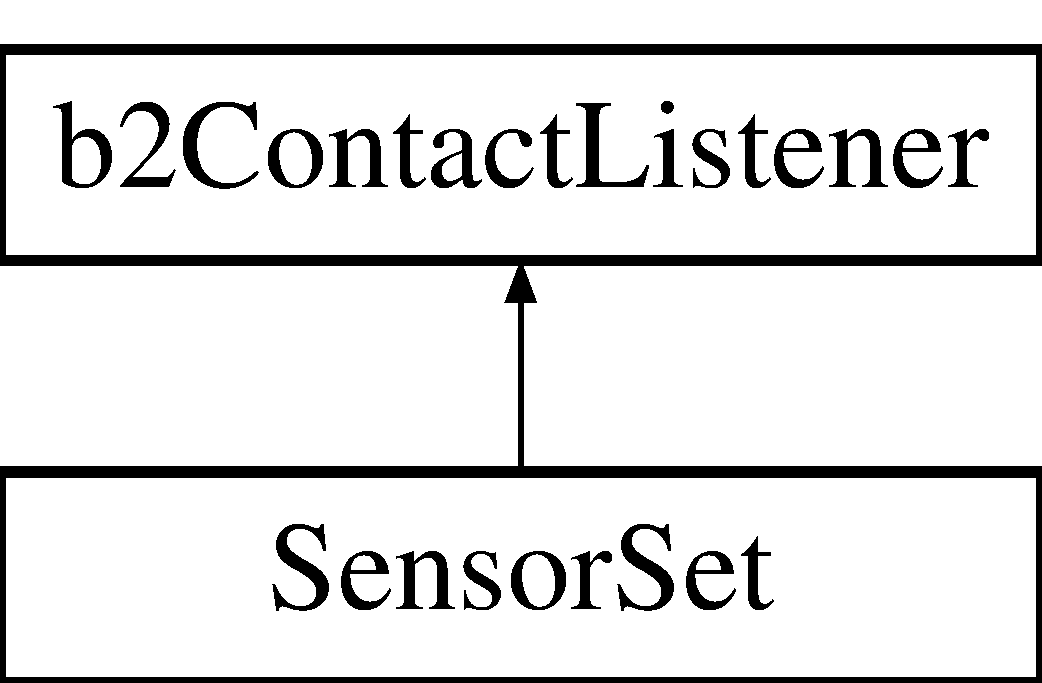
\includegraphics[height=2.000000cm]{classSensorSet}
\end{center}
\end{figure}
\subsection*{Public Member Functions}
\begin{DoxyCompactItemize}
\item 
\hyperlink{classSensorSet_a2ebeeee6217e89c28ae767afb8cbc43e}{Sensor\-Set} (\hyperlink{classCommunicator}{Communicator} $\ast$communicator)
\item 
void \hyperlink{classSensorSet_aed0ec0b0d635de5ffa1f3a459ebf1a18}{Begin\-Contact} (b2\-Contact $\ast$contact)
\item 
void \hyperlink{classSensorSet_aaf34d48652893b393abe3e2c3e28e191}{End\-Contact} (b2\-Contact $\ast$contact)
\item 
void \hyperlink{classSensorSet_a35829e201b615e086bdb328b22f22ca5}{draw\-Labels} ()
\item 
signed int \hyperlink{classSensorSet_aaa08836d3cad9bbe5bca2f85bac25d9e}{read\-Sensor} (signed int id)
\begin{DoxyCompactList}\small\item\em Read sensor state on demand. \end{DoxyCompactList}\item 
void \hyperlink{classSensorSet_a638d99d8fb36d066c074b05f1dba016d}{add} (\hyperlink{classContactSensor}{Contact\-Sensor} $\ast$contact\-Sensor)
\begin{DoxyCompactList}\small\item\em Add sensor to sensor-\/set. \end{DoxyCompactList}\end{DoxyCompactItemize}
\subsection*{Public Attributes}
\begin{DoxyCompactItemize}
\item 
vector$<$ \hyperlink{classContactSensor}{Contact\-Sensor} $\ast$ $>$ \hyperlink{classSensorSet_a2747d586c016d0fe34645f9ca07a08c6}{m\-\_\-contact\-Sensor\-Vector}
\item 
\hyperlink{classCommunicator}{Communicator} $\ast$ \hyperlink{classSensorSet_a9045b86488810de30e8a5b25fdb1128a}{m\-\_\-communicator}
\begin{DoxyCompactList}\small\item\em The communicator with whom \hyperlink{classSensorSet}{Sensor\-Set} speaks. \end{DoxyCompactList}\end{DoxyCompactItemize}


\subsection{Detailed Description}
Listen to sensors and transmit state-\/changes to the communicator. 

\subsection{Constructor \& Destructor Documentation}
\hypertarget{classSensorSet_a2ebeeee6217e89c28ae767afb8cbc43e}{\index{Sensor\-Set@{Sensor\-Set}!Sensor\-Set@{Sensor\-Set}}
\index{Sensor\-Set@{Sensor\-Set}!SensorSet@{Sensor\-Set}}
\subsubsection[{Sensor\-Set}]{\setlength{\rightskip}{0pt plus 5cm}Sensor\-Set\-::\-Sensor\-Set (
\begin{DoxyParamCaption}
\item[{{\bf Communicator} $\ast$}]{communicator}
\end{DoxyParamCaption}
)}}\label{classSensorSet_a2ebeeee6217e89c28ae767afb8cbc43e}


\subsection{Member Function Documentation}
\hypertarget{classSensorSet_a638d99d8fb36d066c074b05f1dba016d}{\index{Sensor\-Set@{Sensor\-Set}!add@{add}}
\index{add@{add}!SensorSet@{Sensor\-Set}}
\subsubsection[{add}]{\setlength{\rightskip}{0pt plus 5cm}void Sensor\-Set\-::add (
\begin{DoxyParamCaption}
\item[{{\bf Contact\-Sensor} $\ast$}]{contact\-Sensor}
\end{DoxyParamCaption}
)}}\label{classSensorSet_a638d99d8fb36d066c074b05f1dba016d}


Add sensor to sensor-\/set. 

\hypertarget{classSensorSet_aed0ec0b0d635de5ffa1f3a459ebf1a18}{\index{Sensor\-Set@{Sensor\-Set}!Begin\-Contact@{Begin\-Contact}}
\index{Begin\-Contact@{Begin\-Contact}!SensorSet@{Sensor\-Set}}
\subsubsection[{Begin\-Contact}]{\setlength{\rightskip}{0pt plus 5cm}void Sensor\-Set\-::\-Begin\-Contact (
\begin{DoxyParamCaption}
\item[{b2\-Contact $\ast$}]{contact}
\end{DoxyParamCaption}
)}}\label{classSensorSet_aed0ec0b0d635de5ffa1f3a459ebf1a18}
\hypertarget{classSensorSet_a35829e201b615e086bdb328b22f22ca5}{\index{Sensor\-Set@{Sensor\-Set}!draw\-Labels@{draw\-Labels}}
\index{draw\-Labels@{draw\-Labels}!SensorSet@{Sensor\-Set}}
\subsubsection[{draw\-Labels}]{\setlength{\rightskip}{0pt plus 5cm}void Sensor\-Set\-::draw\-Labels (
\begin{DoxyParamCaption}
{}
\end{DoxyParamCaption}
)}}\label{classSensorSet_a35829e201b615e086bdb328b22f22ca5}
Draw all sensor labels \hypertarget{classSensorSet_aaf34d48652893b393abe3e2c3e28e191}{\index{Sensor\-Set@{Sensor\-Set}!End\-Contact@{End\-Contact}}
\index{End\-Contact@{End\-Contact}!SensorSet@{Sensor\-Set}}
\subsubsection[{End\-Contact}]{\setlength{\rightskip}{0pt plus 5cm}void Sensor\-Set\-::\-End\-Contact (
\begin{DoxyParamCaption}
\item[{b2\-Contact $\ast$}]{contact}
\end{DoxyParamCaption}
)}}\label{classSensorSet_aaf34d48652893b393abe3e2c3e28e191}
\hypertarget{classSensorSet_aaa08836d3cad9bbe5bca2f85bac25d9e}{\index{Sensor\-Set@{Sensor\-Set}!read\-Sensor@{read\-Sensor}}
\index{read\-Sensor@{read\-Sensor}!SensorSet@{Sensor\-Set}}
\subsubsection[{read\-Sensor}]{\setlength{\rightskip}{0pt plus 5cm}signed int Sensor\-Set\-::read\-Sensor (
\begin{DoxyParamCaption}
\item[{signed int}]{id}
\end{DoxyParamCaption}
)}}\label{classSensorSet_aaa08836d3cad9bbe5bca2f85bac25d9e}


Read sensor state on demand. 



\subsection{Member Data Documentation}
\hypertarget{classSensorSet_a9045b86488810de30e8a5b25fdb1128a}{\index{Sensor\-Set@{Sensor\-Set}!m\-\_\-communicator@{m\-\_\-communicator}}
\index{m\-\_\-communicator@{m\-\_\-communicator}!SensorSet@{Sensor\-Set}}
\subsubsection[{m\-\_\-communicator}]{\setlength{\rightskip}{0pt plus 5cm}{\bf Communicator}$\ast$ Sensor\-Set\-::m\-\_\-communicator}}\label{classSensorSet_a9045b86488810de30e8a5b25fdb1128a}


The communicator with whom \hyperlink{classSensorSet}{Sensor\-Set} speaks. 

\hypertarget{classSensorSet_a2747d586c016d0fe34645f9ca07a08c6}{\index{Sensor\-Set@{Sensor\-Set}!m\-\_\-contact\-Sensor\-Vector@{m\-\_\-contact\-Sensor\-Vector}}
\index{m\-\_\-contact\-Sensor\-Vector@{m\-\_\-contact\-Sensor\-Vector}!SensorSet@{Sensor\-Set}}
\subsubsection[{m\-\_\-contact\-Sensor\-Vector}]{\setlength{\rightskip}{0pt plus 5cm}vector$<${\bf Contact\-Sensor}$\ast$$>$ Sensor\-Set\-::m\-\_\-contact\-Sensor\-Vector}}\label{classSensorSet_a2747d586c016d0fe34645f9ca07a08c6}


The documentation for this class was generated from the following files\-:\begin{DoxyCompactItemize}
\item 
\hyperlink{Sensors_8h}{Sensors.\-h}\item 
\hyperlink{Sensors_8cpp}{Sensors.\-cpp}\end{DoxyCompactItemize}

\hypertarget{structSettings}{\section{Settings Struct Reference}
\label{structSettings}\index{Settings@{Settings}}
}


\hyperlink{classSimulatorPage}{Simulator\-Page} settings. Some can be controlled in the G\-U\-I.  




{\ttfamily \#include $<$Simulator\-Page.\-h$>$}

\subsection*{Public Member Functions}
\begin{DoxyCompactItemize}
\item 
\hyperlink{structSettings_ab7169a6eefce79566dd07db3b1e5e967}{Settings} ()
\end{DoxyCompactItemize}
\subsection*{Public Attributes}
\begin{DoxyCompactItemize}
\item 
b2\-Vec2 \hyperlink{structSettings_a9f73ff7bfe24c0ec00f00637ad660afa}{view\-Center}
\item 
float32 \hyperlink{structSettings_a81f52938e3bfe4976755e77e940ca0e0}{hz}
\item 
int32 \hyperlink{structSettings_aef56168e9043d5a6f264a57fc0d0823a}{velocity\-Iterations}
\item 
int32 \hyperlink{structSettings_ae66b1defd12295dd5dce2362fcdad12f}{position\-Iterations}
\item 
int32 \hyperlink{structSettings_a4a8172dd21368b12a8442723f30914bf}{draw\-Shapes}
\item 
int32 \hyperlink{structSettings_ab03e798642ff7d039d5efa3e0d5e86cb}{draw\-Joints}
\item 
int32 \hyperlink{structSettings_a7ac6f10e3c8e20e8e9a7b7fa90f4b5b5}{draw\-A\-A\-B\-Bs}
\item 
int32 \hyperlink{structSettings_a393ea9824e615323134a9f8514d51ef7}{draw\-Pairs}
\item 
int32 \hyperlink{structSettings_afdc2b5f2611fc52d082e2ff69242cd9b}{draw\-Contact\-Points}
\item 
int32 \hyperlink{structSettings_ad95473a203267e76c613f3a7c2677836}{draw\-Contact\-Normals}
\item 
int32 \hyperlink{structSettings_a55646015c8d056282396c5a8511bc99a}{draw\-Contact\-Forces}
\item 
int32 \hyperlink{structSettings_a9a5046eae0535fff1e23479d18ecaa15}{draw\-Friction\-Forces}
\item 
int32 \hyperlink{structSettings_af5595d1914a8f3b76b43224cc16f05fc}{draw\-C\-O\-Ms}
\item 
int32 \hyperlink{structSettings_ac1dc47bd42cb02ab564d16973c3ac235}{draw\-Stats}
\item 
int32 \hyperlink{structSettings_ab2f2f8bbbd3cf9997000d229f4caff31}{draw\-Profile}
\item 
int32 \hyperlink{structSettings_adb8ab5ccbdefc201db87e2d451df1758}{enable\-Warm\-Starting}
\item 
int32 \hyperlink{structSettings_a5c4a2f9de9c8934d149dc352fc600bf1}{enable\-Continuous}
\item 
int32 \hyperlink{structSettings_a13446b165febfb28b59adcce030d29cc}{enable\-Sub\-Stepping}
\item 
int32 \hyperlink{structSettings_a8be95d53012a813806bd14fdf3d02885}{pause}
\item 
int32 \hyperlink{structSettings_ab26356e864848394be4ae8bc76850d05}{single\-Step}
\end{DoxyCompactItemize}


\subsection{Detailed Description}
\hyperlink{classSimulatorPage}{Simulator\-Page} settings. Some can be controlled in the G\-U\-I. 

\subsection{Constructor \& Destructor Documentation}
\hypertarget{structSettings_ab7169a6eefce79566dd07db3b1e5e967}{\index{Settings@{Settings}!Settings@{Settings}}
\index{Settings@{Settings}!Settings@{Settings}}
\subsubsection[{Settings}]{\setlength{\rightskip}{0pt plus 5cm}Settings\-::\-Settings (
\begin{DoxyParamCaption}
{}
\end{DoxyParamCaption}
)\hspace{0.3cm}{\ttfamily [inline]}}}\label{structSettings_ab7169a6eefce79566dd07db3b1e5e967}


\subsection{Member Data Documentation}
\hypertarget{structSettings_a7ac6f10e3c8e20e8e9a7b7fa90f4b5b5}{\index{Settings@{Settings}!draw\-A\-A\-B\-Bs@{draw\-A\-A\-B\-Bs}}
\index{draw\-A\-A\-B\-Bs@{draw\-A\-A\-B\-Bs}!Settings@{Settings}}
\subsubsection[{draw\-A\-A\-B\-Bs}]{\setlength{\rightskip}{0pt plus 5cm}int32 Settings\-::draw\-A\-A\-B\-Bs}}\label{structSettings_a7ac6f10e3c8e20e8e9a7b7fa90f4b5b5}
\hypertarget{structSettings_af5595d1914a8f3b76b43224cc16f05fc}{\index{Settings@{Settings}!draw\-C\-O\-Ms@{draw\-C\-O\-Ms}}
\index{draw\-C\-O\-Ms@{draw\-C\-O\-Ms}!Settings@{Settings}}
\subsubsection[{draw\-C\-O\-Ms}]{\setlength{\rightskip}{0pt plus 5cm}int32 Settings\-::draw\-C\-O\-Ms}}\label{structSettings_af5595d1914a8f3b76b43224cc16f05fc}
\hypertarget{structSettings_a55646015c8d056282396c5a8511bc99a}{\index{Settings@{Settings}!draw\-Contact\-Forces@{draw\-Contact\-Forces}}
\index{draw\-Contact\-Forces@{draw\-Contact\-Forces}!Settings@{Settings}}
\subsubsection[{draw\-Contact\-Forces}]{\setlength{\rightskip}{0pt plus 5cm}int32 Settings\-::draw\-Contact\-Forces}}\label{structSettings_a55646015c8d056282396c5a8511bc99a}
\hypertarget{structSettings_ad95473a203267e76c613f3a7c2677836}{\index{Settings@{Settings}!draw\-Contact\-Normals@{draw\-Contact\-Normals}}
\index{draw\-Contact\-Normals@{draw\-Contact\-Normals}!Settings@{Settings}}
\subsubsection[{draw\-Contact\-Normals}]{\setlength{\rightskip}{0pt plus 5cm}int32 Settings\-::draw\-Contact\-Normals}}\label{structSettings_ad95473a203267e76c613f3a7c2677836}
\hypertarget{structSettings_afdc2b5f2611fc52d082e2ff69242cd9b}{\index{Settings@{Settings}!draw\-Contact\-Points@{draw\-Contact\-Points}}
\index{draw\-Contact\-Points@{draw\-Contact\-Points}!Settings@{Settings}}
\subsubsection[{draw\-Contact\-Points}]{\setlength{\rightskip}{0pt plus 5cm}int32 Settings\-::draw\-Contact\-Points}}\label{structSettings_afdc2b5f2611fc52d082e2ff69242cd9b}
\hypertarget{structSettings_a9a5046eae0535fff1e23479d18ecaa15}{\index{Settings@{Settings}!draw\-Friction\-Forces@{draw\-Friction\-Forces}}
\index{draw\-Friction\-Forces@{draw\-Friction\-Forces}!Settings@{Settings}}
\subsubsection[{draw\-Friction\-Forces}]{\setlength{\rightskip}{0pt plus 5cm}int32 Settings\-::draw\-Friction\-Forces}}\label{structSettings_a9a5046eae0535fff1e23479d18ecaa15}
\hypertarget{structSettings_ab03e798642ff7d039d5efa3e0d5e86cb}{\index{Settings@{Settings}!draw\-Joints@{draw\-Joints}}
\index{draw\-Joints@{draw\-Joints}!Settings@{Settings}}
\subsubsection[{draw\-Joints}]{\setlength{\rightskip}{0pt plus 5cm}int32 Settings\-::draw\-Joints}}\label{structSettings_ab03e798642ff7d039d5efa3e0d5e86cb}
\hypertarget{structSettings_a393ea9824e615323134a9f8514d51ef7}{\index{Settings@{Settings}!draw\-Pairs@{draw\-Pairs}}
\index{draw\-Pairs@{draw\-Pairs}!Settings@{Settings}}
\subsubsection[{draw\-Pairs}]{\setlength{\rightskip}{0pt plus 5cm}int32 Settings\-::draw\-Pairs}}\label{structSettings_a393ea9824e615323134a9f8514d51ef7}
\hypertarget{structSettings_ab2f2f8bbbd3cf9997000d229f4caff31}{\index{Settings@{Settings}!draw\-Profile@{draw\-Profile}}
\index{draw\-Profile@{draw\-Profile}!Settings@{Settings}}
\subsubsection[{draw\-Profile}]{\setlength{\rightskip}{0pt plus 5cm}int32 Settings\-::draw\-Profile}}\label{structSettings_ab2f2f8bbbd3cf9997000d229f4caff31}
\hypertarget{structSettings_a4a8172dd21368b12a8442723f30914bf}{\index{Settings@{Settings}!draw\-Shapes@{draw\-Shapes}}
\index{draw\-Shapes@{draw\-Shapes}!Settings@{Settings}}
\subsubsection[{draw\-Shapes}]{\setlength{\rightskip}{0pt plus 5cm}int32 Settings\-::draw\-Shapes}}\label{structSettings_a4a8172dd21368b12a8442723f30914bf}
\hypertarget{structSettings_ac1dc47bd42cb02ab564d16973c3ac235}{\index{Settings@{Settings}!draw\-Stats@{draw\-Stats}}
\index{draw\-Stats@{draw\-Stats}!Settings@{Settings}}
\subsubsection[{draw\-Stats}]{\setlength{\rightskip}{0pt plus 5cm}int32 Settings\-::draw\-Stats}}\label{structSettings_ac1dc47bd42cb02ab564d16973c3ac235}
\hypertarget{structSettings_a5c4a2f9de9c8934d149dc352fc600bf1}{\index{Settings@{Settings}!enable\-Continuous@{enable\-Continuous}}
\index{enable\-Continuous@{enable\-Continuous}!Settings@{Settings}}
\subsubsection[{enable\-Continuous}]{\setlength{\rightskip}{0pt plus 5cm}int32 Settings\-::enable\-Continuous}}\label{structSettings_a5c4a2f9de9c8934d149dc352fc600bf1}
\hypertarget{structSettings_a13446b165febfb28b59adcce030d29cc}{\index{Settings@{Settings}!enable\-Sub\-Stepping@{enable\-Sub\-Stepping}}
\index{enable\-Sub\-Stepping@{enable\-Sub\-Stepping}!Settings@{Settings}}
\subsubsection[{enable\-Sub\-Stepping}]{\setlength{\rightskip}{0pt plus 5cm}int32 Settings\-::enable\-Sub\-Stepping}}\label{structSettings_a13446b165febfb28b59adcce030d29cc}
\hypertarget{structSettings_adb8ab5ccbdefc201db87e2d451df1758}{\index{Settings@{Settings}!enable\-Warm\-Starting@{enable\-Warm\-Starting}}
\index{enable\-Warm\-Starting@{enable\-Warm\-Starting}!Settings@{Settings}}
\subsubsection[{enable\-Warm\-Starting}]{\setlength{\rightskip}{0pt plus 5cm}int32 Settings\-::enable\-Warm\-Starting}}\label{structSettings_adb8ab5ccbdefc201db87e2d451df1758}
\hypertarget{structSettings_a81f52938e3bfe4976755e77e940ca0e0}{\index{Settings@{Settings}!hz@{hz}}
\index{hz@{hz}!Settings@{Settings}}
\subsubsection[{hz}]{\setlength{\rightskip}{0pt plus 5cm}float32 Settings\-::hz}}\label{structSettings_a81f52938e3bfe4976755e77e940ca0e0}
\hypertarget{structSettings_a8be95d53012a813806bd14fdf3d02885}{\index{Settings@{Settings}!pause@{pause}}
\index{pause@{pause}!Settings@{Settings}}
\subsubsection[{pause}]{\setlength{\rightskip}{0pt plus 5cm}int32 Settings\-::pause}}\label{structSettings_a8be95d53012a813806bd14fdf3d02885}
\hypertarget{structSettings_ae66b1defd12295dd5dce2362fcdad12f}{\index{Settings@{Settings}!position\-Iterations@{position\-Iterations}}
\index{position\-Iterations@{position\-Iterations}!Settings@{Settings}}
\subsubsection[{position\-Iterations}]{\setlength{\rightskip}{0pt plus 5cm}int32 Settings\-::position\-Iterations}}\label{structSettings_ae66b1defd12295dd5dce2362fcdad12f}
\hypertarget{structSettings_ab26356e864848394be4ae8bc76850d05}{\index{Settings@{Settings}!single\-Step@{single\-Step}}
\index{single\-Step@{single\-Step}!Settings@{Settings}}
\subsubsection[{single\-Step}]{\setlength{\rightskip}{0pt plus 5cm}int32 Settings\-::single\-Step}}\label{structSettings_ab26356e864848394be4ae8bc76850d05}
\hypertarget{structSettings_aef56168e9043d5a6f264a57fc0d0823a}{\index{Settings@{Settings}!velocity\-Iterations@{velocity\-Iterations}}
\index{velocity\-Iterations@{velocity\-Iterations}!Settings@{Settings}}
\subsubsection[{velocity\-Iterations}]{\setlength{\rightskip}{0pt plus 5cm}int32 Settings\-::velocity\-Iterations}}\label{structSettings_aef56168e9043d5a6f264a57fc0d0823a}
\hypertarget{structSettings_a9f73ff7bfe24c0ec00f00637ad660afa}{\index{Settings@{Settings}!view\-Center@{view\-Center}}
\index{view\-Center@{view\-Center}!Settings@{Settings}}
\subsubsection[{view\-Center}]{\setlength{\rightskip}{0pt plus 5cm}b2\-Vec2 Settings\-::view\-Center}}\label{structSettings_a9f73ff7bfe24c0ec00f00637ad660afa}


The documentation for this struct was generated from the following file\-:\begin{DoxyCompactItemize}
\item 
\hyperlink{SimulatorPage_8h}{Simulator\-Page.\-h}\end{DoxyCompactItemize}

\hypertarget{classSimulatorPage}{\section{Simulator\-Page Class Reference}
\label{classSimulatorPage}\index{Simulator\-Page@{Simulator\-Page}}
}


{\ttfamily \#include $<$Simulator\-Page.\-h$>$}

Inheritance diagram for Simulator\-Page\-:\begin{figure}[H]
\begin{center}
\leavevmode
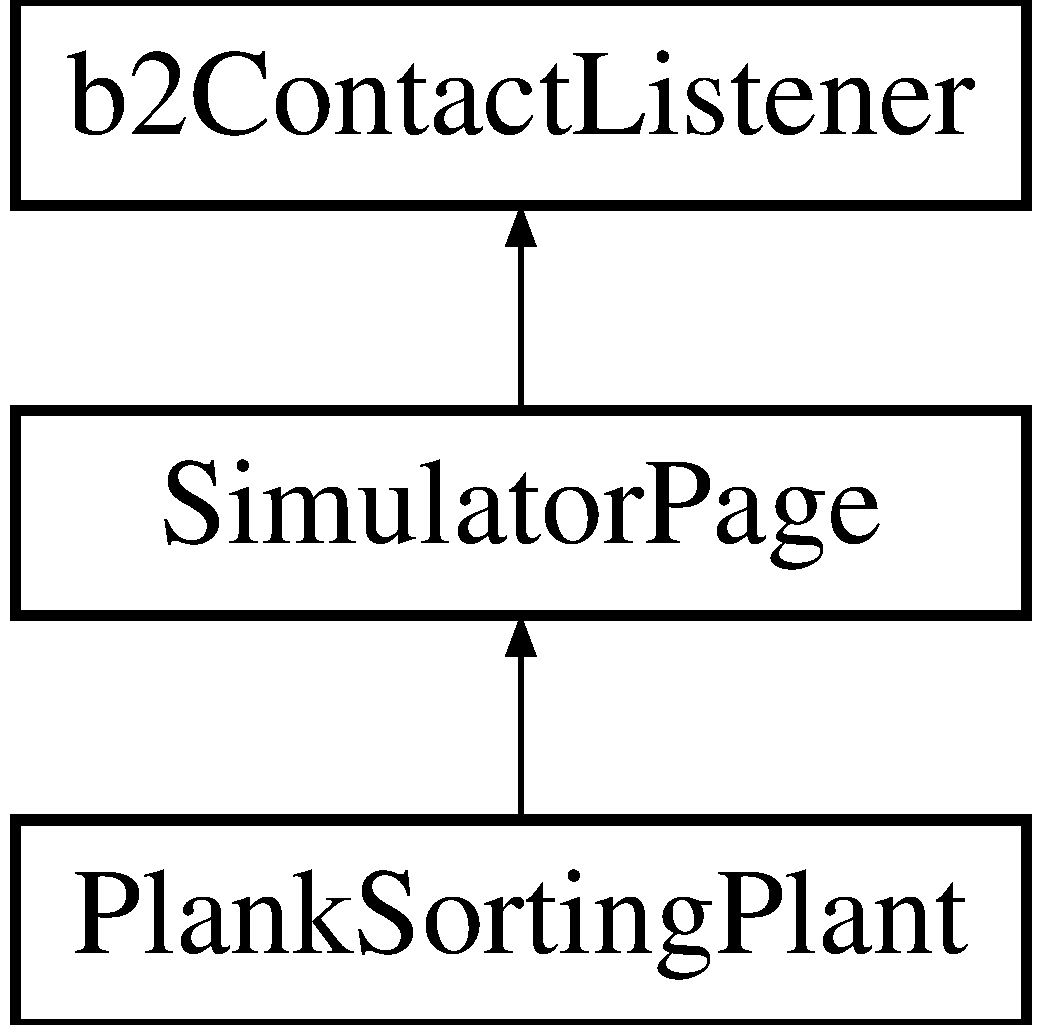
\includegraphics[height=3.000000cm]{classSimulatorPage}
\end{center}
\end{figure}
\subsection*{Public Member Functions}
\begin{DoxyCompactItemize}
\item 
\hyperlink{classSimulatorPage_ae4c224aee18df3d96f37b54a0bf36464}{Simulator\-Page} (\hyperlink{classCommunicator}{Communicator} $\ast$communicator)
\item 
virtual \hyperlink{classSimulatorPage_af1468b91ff43c04bf51596769553ff5a}{$\sim$\-Simulator\-Page} ()
\item 
void \hyperlink{classSimulatorPage_af9089342514e16944fbc9f6202ed1439}{Set\-Text\-Line} (int32 line)
\item 
void \hyperlink{classSimulatorPage_a9bb317b7301bb3fddfd0bda065447d80}{Draw\-Title} (int x, int y, const char $\ast$string)
\item 
virtual void \hyperlink{classSimulatorPage_ac478dc8792d0f593c6dc6277a4e96719}{Step} (\hyperlink{structSettings}{Settings} $\ast$settings)
\item 
virtual void \hyperlink{classSimulatorPage_a295bcbd72dfe0dd651d922b8165e8f9a}{Keyboard} (unsigned char key)
\item 
virtual void \hyperlink{classSimulatorPage_af95e71d2e0b7bad8d0cdf7b7e5588440}{Keyboard\-Up} (unsigned char key)
\item 
void \hyperlink{classSimulatorPage_aa780589b43ed6c51d5d293b004dfd695}{Shift\-Mouse\-Down} (const b2\-Vec2 \&p)
\item 
virtual void \hyperlink{classSimulatorPage_ad6c49283fed786a374af8a3f236b2e29}{Mouse\-Down} (const b2\-Vec2 \&p)
\item 
virtual void \hyperlink{classSimulatorPage_afcc118e0e87b65a2c4bf95a76cec2396}{Mouse\-Up} (const b2\-Vec2 \&p)
\item 
void \hyperlink{classSimulatorPage_a71ff43bcbced024eaa85b037a9c22006}{Mouse\-Move} (const b2\-Vec2 \&p)
\item 
void \hyperlink{classSimulatorPage_a39e3534423f49c6f6f233b81f7f5bc80}{Launch\-Bomb} ()
\item 
void \hyperlink{classSimulatorPage_a99976c3f608eb764bee788460b2c0f8d}{Launch\-Bomb} (const b2\-Vec2 \&position, const b2\-Vec2 \&velocity)
\item 
void \hyperlink{classSimulatorPage_a177d0ac170bcdd4ec523ce0c99dec40d}{Spawn\-Bomb} (const b2\-Vec2 \&world\-Pt)
\item 
void \hyperlink{classSimulatorPage_a25475c39d60beeabfa7c5bf0f9bbaae9}{Complete\-Bomb\-Spawn} (const b2\-Vec2 \&p)
\item 
virtual void \hyperlink{classSimulatorPage_a1c6a3e2ebc71dcc01aaebca77fcec421}{Joint\-Destroyed} (b2\-Joint $\ast$joint)
\item 
virtual void \hyperlink{classSimulatorPage_a5a6ea36613740fcbb301317ac48816b0}{Begin\-Contact} (b2\-Contact $\ast$contact)
\item 
virtual void \hyperlink{classSimulatorPage_a1679b66b418b92aafb7e46a47c737f03}{End\-Contact} (b2\-Contact $\ast$contact)
\item 
virtual void \hyperlink{classSimulatorPage_a0bf3450167587c8f2e013df17abecb73}{Pre\-Solve} (b2\-Contact $\ast$contact, const b2\-Manifold $\ast$old\-Manifold)
\item 
virtual void \hyperlink{classSimulatorPage_aa86fc16964e2465873d3b352d70a6ae6}{Post\-Solve} (const b2\-Contact $\ast$contact, const b2\-Contact\-Impulse $\ast$impulse)
\end{DoxyCompactItemize}
\subsection*{Protected Attributes}
\begin{DoxyCompactItemize}
\item 
b2\-Body $\ast$ \hyperlink{classSimulatorPage_ab4c6f15c6a33d3884c3e3a55b93971ec}{m\-\_\-ground\-Body}
\item 
b2\-A\-A\-B\-B \hyperlink{classSimulatorPage_afe7bd14c770a28ab335a803ebc93d1a5}{m\-\_\-world\-A\-A\-B\-B}
\item 
\hyperlink{structContactPoint}{Contact\-Point} \hyperlink{classSimulatorPage_afa967705601096830dc2bb2a0fd3b999}{m\-\_\-points} \mbox{[}\hyperlink{SimulatorPage_8h_ae34d209729703751560149e5bcb5d2f0}{k\-\_\-max\-Contact\-Points}\mbox{]}
\item 
int32 \hyperlink{classSimulatorPage_a26946c6050b34954b256c4b0271be534}{m\-\_\-point\-Count}
\item 
\hyperlink{classDestructionListener}{Destruction\-Listener} \hyperlink{classSimulatorPage_a3fd7bc3de5a63d35d152f8446f41cd53}{m\-\_\-destruction\-Listener}
\item 
\hyperlink{classDebugDraw}{Debug\-Draw} \hyperlink{classSimulatorPage_a9b074b47b00e81c08154cf2975282a6d}{m\-\_\-debug\-Draw}
\item 
int32 \hyperlink{classSimulatorPage_aebe43734cac8bf5c8a88fb20e0975b63}{m\-\_\-text\-Line}
\item 
b2\-World $\ast$ \hyperlink{classSimulatorPage_af1b8c6fc0d7ede12a5132fe44c0fae5e}{m\-\_\-world}
\item 
b2\-Body $\ast$ \hyperlink{classSimulatorPage_a9ecb370ad58655cbc55190869fe43fab}{m\-\_\-bomb}
\item 
b2\-Mouse\-Joint $\ast$ \hyperlink{classSimulatorPage_a1dd1eef1ae65277d3bd5e93c44baca03}{m\-\_\-mouse\-Joint}
\item 
b2\-Vec2 \hyperlink{classSimulatorPage_a1be96eadc8befadc61960d68e602238a}{m\-\_\-bomb\-Spawn\-Point}
\item 
bool \hyperlink{classSimulatorPage_a5140893531a64b6fdf035b0c1ab448eb}{m\-\_\-bomb\-Spawning}
\item 
b2\-Vec2 \hyperlink{classSimulatorPage_aba988f418bc061a8d70982589916f662}{m\-\_\-mouse\-World}
\item 
int32 \hyperlink{classSimulatorPage_ac9a5a37acf3ec09e34983fe661ec5d3c}{m\-\_\-step\-Count}
\item 
b2\-Profile \hyperlink{classSimulatorPage_a715c353347e2e677ac7e4dadfe3b0792}{m\-\_\-max\-Profile}
\item 
b2\-Profile \hyperlink{classSimulatorPage_a53d76f9f1cd19e16205223d0277a878d}{m\-\_\-total\-Profile}
\item 
\hyperlink{classCommunicator}{Communicator} $\ast$ \hyperlink{classSimulatorPage_a26c6d51e11a440700f8400da277926b1}{m\-\_\-communicator}
\end{DoxyCompactItemize}
\subsection*{Friends}
\begin{DoxyCompactItemize}
\item 
class \hyperlink{classSimulatorPage_a070117113adbe4bd234cc819a8a31d67}{Destruction\-Listener}
\item 
class \hyperlink{classSimulatorPage_ace42de2cf55b34c2abc668b911b4fc70}{Boundary\-Listener}
\item 
class \hyperlink{classSimulatorPage_aea5531aaede6e9afc2c156b067c847d4}{Contact\-Listener}
\end{DoxyCompactItemize}


\subsection{Constructor \& Destructor Documentation}
\hypertarget{classSimulatorPage_ae4c224aee18df3d96f37b54a0bf36464}{\index{Simulator\-Page@{Simulator\-Page}!Simulator\-Page@{Simulator\-Page}}
\index{Simulator\-Page@{Simulator\-Page}!SimulatorPage@{Simulator\-Page}}
\subsubsection[{Simulator\-Page}]{\setlength{\rightskip}{0pt plus 5cm}Simulator\-Page\-::\-Simulator\-Page (
\begin{DoxyParamCaption}
\item[{{\bf Communicator} $\ast$}]{communicator}
\end{DoxyParamCaption}
)}}\label{classSimulatorPage_ae4c224aee18df3d96f37b54a0bf36464}
\hypertarget{classSimulatorPage_af1468b91ff43c04bf51596769553ff5a}{\index{Simulator\-Page@{Simulator\-Page}!$\sim$\-Simulator\-Page@{$\sim$\-Simulator\-Page}}
\index{$\sim$\-Simulator\-Page@{$\sim$\-Simulator\-Page}!SimulatorPage@{Simulator\-Page}}
\subsubsection[{$\sim$\-Simulator\-Page}]{\setlength{\rightskip}{0pt plus 5cm}Simulator\-Page\-::$\sim$\-Simulator\-Page (
\begin{DoxyParamCaption}
{}
\end{DoxyParamCaption}
)\hspace{0.3cm}{\ttfamily [virtual]}}}\label{classSimulatorPage_af1468b91ff43c04bf51596769553ff5a}


\subsection{Member Function Documentation}
\hypertarget{classSimulatorPage_a5a6ea36613740fcbb301317ac48816b0}{\index{Simulator\-Page@{Simulator\-Page}!Begin\-Contact@{Begin\-Contact}}
\index{Begin\-Contact@{Begin\-Contact}!SimulatorPage@{Simulator\-Page}}
\subsubsection[{Begin\-Contact}]{\setlength{\rightskip}{0pt plus 5cm}virtual void Simulator\-Page\-::\-Begin\-Contact (
\begin{DoxyParamCaption}
\item[{b2\-Contact $\ast$}]{contact}
\end{DoxyParamCaption}
)\hspace{0.3cm}{\ttfamily [inline]}, {\ttfamily [virtual]}}}\label{classSimulatorPage_a5a6ea36613740fcbb301317ac48816b0}
\hypertarget{classSimulatorPage_a25475c39d60beeabfa7c5bf0f9bbaae9}{\index{Simulator\-Page@{Simulator\-Page}!Complete\-Bomb\-Spawn@{Complete\-Bomb\-Spawn}}
\index{Complete\-Bomb\-Spawn@{Complete\-Bomb\-Spawn}!SimulatorPage@{Simulator\-Page}}
\subsubsection[{Complete\-Bomb\-Spawn}]{\setlength{\rightskip}{0pt plus 5cm}void Simulator\-Page\-::\-Complete\-Bomb\-Spawn (
\begin{DoxyParamCaption}
\item[{const b2\-Vec2 \&}]{p}
\end{DoxyParamCaption}
)}}\label{classSimulatorPage_a25475c39d60beeabfa7c5bf0f9bbaae9}
\hypertarget{classSimulatorPage_a9bb317b7301bb3fddfd0bda065447d80}{\index{Simulator\-Page@{Simulator\-Page}!Draw\-Title@{Draw\-Title}}
\index{Draw\-Title@{Draw\-Title}!SimulatorPage@{Simulator\-Page}}
\subsubsection[{Draw\-Title}]{\setlength{\rightskip}{0pt plus 5cm}void Simulator\-Page\-::\-Draw\-Title (
\begin{DoxyParamCaption}
\item[{int}]{x, }
\item[{int}]{y, }
\item[{const char $\ast$}]{string}
\end{DoxyParamCaption}
)}}\label{classSimulatorPage_a9bb317b7301bb3fddfd0bda065447d80}
\hypertarget{classSimulatorPage_a1679b66b418b92aafb7e46a47c737f03}{\index{Simulator\-Page@{Simulator\-Page}!End\-Contact@{End\-Contact}}
\index{End\-Contact@{End\-Contact}!SimulatorPage@{Simulator\-Page}}
\subsubsection[{End\-Contact}]{\setlength{\rightskip}{0pt plus 5cm}virtual void Simulator\-Page\-::\-End\-Contact (
\begin{DoxyParamCaption}
\item[{b2\-Contact $\ast$}]{contact}
\end{DoxyParamCaption}
)\hspace{0.3cm}{\ttfamily [inline]}, {\ttfamily [virtual]}}}\label{classSimulatorPage_a1679b66b418b92aafb7e46a47c737f03}
\hypertarget{classSimulatorPage_a1c6a3e2ebc71dcc01aaebca77fcec421}{\index{Simulator\-Page@{Simulator\-Page}!Joint\-Destroyed@{Joint\-Destroyed}}
\index{Joint\-Destroyed@{Joint\-Destroyed}!SimulatorPage@{Simulator\-Page}}
\subsubsection[{Joint\-Destroyed}]{\setlength{\rightskip}{0pt plus 5cm}virtual void Simulator\-Page\-::\-Joint\-Destroyed (
\begin{DoxyParamCaption}
\item[{b2\-Joint $\ast$}]{joint}
\end{DoxyParamCaption}
)\hspace{0.3cm}{\ttfamily [inline]}, {\ttfamily [virtual]}}}\label{classSimulatorPage_a1c6a3e2ebc71dcc01aaebca77fcec421}
\hypertarget{classSimulatorPage_a295bcbd72dfe0dd651d922b8165e8f9a}{\index{Simulator\-Page@{Simulator\-Page}!Keyboard@{Keyboard}}
\index{Keyboard@{Keyboard}!SimulatorPage@{Simulator\-Page}}
\subsubsection[{Keyboard}]{\setlength{\rightskip}{0pt plus 5cm}virtual void Simulator\-Page\-::\-Keyboard (
\begin{DoxyParamCaption}
\item[{unsigned char}]{key}
\end{DoxyParamCaption}
)\hspace{0.3cm}{\ttfamily [inline]}, {\ttfamily [virtual]}}}\label{classSimulatorPage_a295bcbd72dfe0dd651d922b8165e8f9a}


Reimplemented in \hyperlink{classPlankSortingPlant_a131fade1b547a3af4f2b5158bc285e30}{Plank\-Sorting\-Plant}.

\hypertarget{classSimulatorPage_af95e71d2e0b7bad8d0cdf7b7e5588440}{\index{Simulator\-Page@{Simulator\-Page}!Keyboard\-Up@{Keyboard\-Up}}
\index{Keyboard\-Up@{Keyboard\-Up}!SimulatorPage@{Simulator\-Page}}
\subsubsection[{Keyboard\-Up}]{\setlength{\rightskip}{0pt plus 5cm}virtual void Simulator\-Page\-::\-Keyboard\-Up (
\begin{DoxyParamCaption}
\item[{unsigned char}]{key}
\end{DoxyParamCaption}
)\hspace{0.3cm}{\ttfamily [inline]}, {\ttfamily [virtual]}}}\label{classSimulatorPage_af95e71d2e0b7bad8d0cdf7b7e5588440}
\hypertarget{classSimulatorPage_a39e3534423f49c6f6f233b81f7f5bc80}{\index{Simulator\-Page@{Simulator\-Page}!Launch\-Bomb@{Launch\-Bomb}}
\index{Launch\-Bomb@{Launch\-Bomb}!SimulatorPage@{Simulator\-Page}}
\subsubsection[{Launch\-Bomb}]{\setlength{\rightskip}{0pt plus 5cm}void Simulator\-Page\-::\-Launch\-Bomb (
\begin{DoxyParamCaption}
{}
\end{DoxyParamCaption}
)}}\label{classSimulatorPage_a39e3534423f49c6f6f233b81f7f5bc80}
\hypertarget{classSimulatorPage_a99976c3f608eb764bee788460b2c0f8d}{\index{Simulator\-Page@{Simulator\-Page}!Launch\-Bomb@{Launch\-Bomb}}
\index{Launch\-Bomb@{Launch\-Bomb}!SimulatorPage@{Simulator\-Page}}
\subsubsection[{Launch\-Bomb}]{\setlength{\rightskip}{0pt plus 5cm}void Simulator\-Page\-::\-Launch\-Bomb (
\begin{DoxyParamCaption}
\item[{const b2\-Vec2 \&}]{position, }
\item[{const b2\-Vec2 \&}]{velocity}
\end{DoxyParamCaption}
)}}\label{classSimulatorPage_a99976c3f608eb764bee788460b2c0f8d}
\hypertarget{classSimulatorPage_ad6c49283fed786a374af8a3f236b2e29}{\index{Simulator\-Page@{Simulator\-Page}!Mouse\-Down@{Mouse\-Down}}
\index{Mouse\-Down@{Mouse\-Down}!SimulatorPage@{Simulator\-Page}}
\subsubsection[{Mouse\-Down}]{\setlength{\rightskip}{0pt plus 5cm}void Simulator\-Page\-::\-Mouse\-Down (
\begin{DoxyParamCaption}
\item[{const b2\-Vec2 \&}]{p}
\end{DoxyParamCaption}
)\hspace{0.3cm}{\ttfamily [virtual]}}}\label{classSimulatorPage_ad6c49283fed786a374af8a3f236b2e29}
\hypertarget{classSimulatorPage_a71ff43bcbced024eaa85b037a9c22006}{\index{Simulator\-Page@{Simulator\-Page}!Mouse\-Move@{Mouse\-Move}}
\index{Mouse\-Move@{Mouse\-Move}!SimulatorPage@{Simulator\-Page}}
\subsubsection[{Mouse\-Move}]{\setlength{\rightskip}{0pt plus 5cm}void Simulator\-Page\-::\-Mouse\-Move (
\begin{DoxyParamCaption}
\item[{const b2\-Vec2 \&}]{p}
\end{DoxyParamCaption}
)}}\label{classSimulatorPage_a71ff43bcbced024eaa85b037a9c22006}
\hypertarget{classSimulatorPage_afcc118e0e87b65a2c4bf95a76cec2396}{\index{Simulator\-Page@{Simulator\-Page}!Mouse\-Up@{Mouse\-Up}}
\index{Mouse\-Up@{Mouse\-Up}!SimulatorPage@{Simulator\-Page}}
\subsubsection[{Mouse\-Up}]{\setlength{\rightskip}{0pt plus 5cm}void Simulator\-Page\-::\-Mouse\-Up (
\begin{DoxyParamCaption}
\item[{const b2\-Vec2 \&}]{p}
\end{DoxyParamCaption}
)\hspace{0.3cm}{\ttfamily [virtual]}}}\label{classSimulatorPage_afcc118e0e87b65a2c4bf95a76cec2396}
\hypertarget{classSimulatorPage_aa86fc16964e2465873d3b352d70a6ae6}{\index{Simulator\-Page@{Simulator\-Page}!Post\-Solve@{Post\-Solve}}
\index{Post\-Solve@{Post\-Solve}!SimulatorPage@{Simulator\-Page}}
\subsubsection[{Post\-Solve}]{\setlength{\rightskip}{0pt plus 5cm}virtual void Simulator\-Page\-::\-Post\-Solve (
\begin{DoxyParamCaption}
\item[{const b2\-Contact $\ast$}]{contact, }
\item[{const b2\-Contact\-Impulse $\ast$}]{impulse}
\end{DoxyParamCaption}
)\hspace{0.3cm}{\ttfamily [inline]}, {\ttfamily [virtual]}}}\label{classSimulatorPage_aa86fc16964e2465873d3b352d70a6ae6}
\hypertarget{classSimulatorPage_a0bf3450167587c8f2e013df17abecb73}{\index{Simulator\-Page@{Simulator\-Page}!Pre\-Solve@{Pre\-Solve}}
\index{Pre\-Solve@{Pre\-Solve}!SimulatorPage@{Simulator\-Page}}
\subsubsection[{Pre\-Solve}]{\setlength{\rightskip}{0pt plus 5cm}void Simulator\-Page\-::\-Pre\-Solve (
\begin{DoxyParamCaption}
\item[{b2\-Contact $\ast$}]{contact, }
\item[{const b2\-Manifold $\ast$}]{old\-Manifold}
\end{DoxyParamCaption}
)\hspace{0.3cm}{\ttfamily [virtual]}}}\label{classSimulatorPage_a0bf3450167587c8f2e013df17abecb73}
\hypertarget{classSimulatorPage_af9089342514e16944fbc9f6202ed1439}{\index{Simulator\-Page@{Simulator\-Page}!Set\-Text\-Line@{Set\-Text\-Line}}
\index{Set\-Text\-Line@{Set\-Text\-Line}!SimulatorPage@{Simulator\-Page}}
\subsubsection[{Set\-Text\-Line}]{\setlength{\rightskip}{0pt plus 5cm}void Simulator\-Page\-::\-Set\-Text\-Line (
\begin{DoxyParamCaption}
\item[{int32}]{line}
\end{DoxyParamCaption}
)\hspace{0.3cm}{\ttfamily [inline]}}}\label{classSimulatorPage_af9089342514e16944fbc9f6202ed1439}
\hypertarget{classSimulatorPage_aa780589b43ed6c51d5d293b004dfd695}{\index{Simulator\-Page@{Simulator\-Page}!Shift\-Mouse\-Down@{Shift\-Mouse\-Down}}
\index{Shift\-Mouse\-Down@{Shift\-Mouse\-Down}!SimulatorPage@{Simulator\-Page}}
\subsubsection[{Shift\-Mouse\-Down}]{\setlength{\rightskip}{0pt plus 5cm}void Simulator\-Page\-::\-Shift\-Mouse\-Down (
\begin{DoxyParamCaption}
\item[{const b2\-Vec2 \&}]{p}
\end{DoxyParamCaption}
)}}\label{classSimulatorPage_aa780589b43ed6c51d5d293b004dfd695}
\hypertarget{classSimulatorPage_a177d0ac170bcdd4ec523ce0c99dec40d}{\index{Simulator\-Page@{Simulator\-Page}!Spawn\-Bomb@{Spawn\-Bomb}}
\index{Spawn\-Bomb@{Spawn\-Bomb}!SimulatorPage@{Simulator\-Page}}
\subsubsection[{Spawn\-Bomb}]{\setlength{\rightskip}{0pt plus 5cm}void Simulator\-Page\-::\-Spawn\-Bomb (
\begin{DoxyParamCaption}
\item[{const b2\-Vec2 \&}]{world\-Pt}
\end{DoxyParamCaption}
)}}\label{classSimulatorPage_a177d0ac170bcdd4ec523ce0c99dec40d}
\hypertarget{classSimulatorPage_ac478dc8792d0f593c6dc6277a4e96719}{\index{Simulator\-Page@{Simulator\-Page}!Step@{Step}}
\index{Step@{Step}!SimulatorPage@{Simulator\-Page}}
\subsubsection[{Step}]{\setlength{\rightskip}{0pt plus 5cm}void Simulator\-Page\-::\-Step (
\begin{DoxyParamCaption}
\item[{{\bf Settings} $\ast$}]{settings}
\end{DoxyParamCaption}
)\hspace{0.3cm}{\ttfamily [virtual]}}}\label{classSimulatorPage_ac478dc8792d0f593c6dc6277a4e96719}


Reimplemented in \hyperlink{classPlankSortingPlant_a512555c258c6e6d824356af6ed2e77f2}{Plank\-Sorting\-Plant}.



\subsection{Friends And Related Function Documentation}
\hypertarget{classSimulatorPage_ace42de2cf55b34c2abc668b911b4fc70}{\index{Simulator\-Page@{Simulator\-Page}!Boundary\-Listener@{Boundary\-Listener}}
\index{Boundary\-Listener@{Boundary\-Listener}!SimulatorPage@{Simulator\-Page}}
\subsubsection[{Boundary\-Listener}]{\setlength{\rightskip}{0pt plus 5cm}friend class Boundary\-Listener\hspace{0.3cm}{\ttfamily [friend]}}}\label{classSimulatorPage_ace42de2cf55b34c2abc668b911b4fc70}
\hypertarget{classSimulatorPage_aea5531aaede6e9afc2c156b067c847d4}{\index{Simulator\-Page@{Simulator\-Page}!Contact\-Listener@{Contact\-Listener}}
\index{Contact\-Listener@{Contact\-Listener}!SimulatorPage@{Simulator\-Page}}
\subsubsection[{Contact\-Listener}]{\setlength{\rightskip}{0pt plus 5cm}friend class Contact\-Listener\hspace{0.3cm}{\ttfamily [friend]}}}\label{classSimulatorPage_aea5531aaede6e9afc2c156b067c847d4}
\hypertarget{classSimulatorPage_a070117113adbe4bd234cc819a8a31d67}{\index{Simulator\-Page@{Simulator\-Page}!Destruction\-Listener@{Destruction\-Listener}}
\index{Destruction\-Listener@{Destruction\-Listener}!SimulatorPage@{Simulator\-Page}}
\subsubsection[{Destruction\-Listener}]{\setlength{\rightskip}{0pt plus 5cm}friend class {\bf Destruction\-Listener}\hspace{0.3cm}{\ttfamily [friend]}}}\label{classSimulatorPage_a070117113adbe4bd234cc819a8a31d67}


\subsection{Member Data Documentation}
\hypertarget{classSimulatorPage_a9ecb370ad58655cbc55190869fe43fab}{\index{Simulator\-Page@{Simulator\-Page}!m\-\_\-bomb@{m\-\_\-bomb}}
\index{m\-\_\-bomb@{m\-\_\-bomb}!SimulatorPage@{Simulator\-Page}}
\subsubsection[{m\-\_\-bomb}]{\setlength{\rightskip}{0pt plus 5cm}b2\-Body$\ast$ Simulator\-Page\-::m\-\_\-bomb\hspace{0.3cm}{\ttfamily [protected]}}}\label{classSimulatorPage_a9ecb370ad58655cbc55190869fe43fab}
\hypertarget{classSimulatorPage_a5140893531a64b6fdf035b0c1ab448eb}{\index{Simulator\-Page@{Simulator\-Page}!m\-\_\-bomb\-Spawning@{m\-\_\-bomb\-Spawning}}
\index{m\-\_\-bomb\-Spawning@{m\-\_\-bomb\-Spawning}!SimulatorPage@{Simulator\-Page}}
\subsubsection[{m\-\_\-bomb\-Spawning}]{\setlength{\rightskip}{0pt plus 5cm}bool Simulator\-Page\-::m\-\_\-bomb\-Spawning\hspace{0.3cm}{\ttfamily [protected]}}}\label{classSimulatorPage_a5140893531a64b6fdf035b0c1ab448eb}
\hypertarget{classSimulatorPage_a1be96eadc8befadc61960d68e602238a}{\index{Simulator\-Page@{Simulator\-Page}!m\-\_\-bomb\-Spawn\-Point@{m\-\_\-bomb\-Spawn\-Point}}
\index{m\-\_\-bomb\-Spawn\-Point@{m\-\_\-bomb\-Spawn\-Point}!SimulatorPage@{Simulator\-Page}}
\subsubsection[{m\-\_\-bomb\-Spawn\-Point}]{\setlength{\rightskip}{0pt plus 5cm}b2\-Vec2 Simulator\-Page\-::m\-\_\-bomb\-Spawn\-Point\hspace{0.3cm}{\ttfamily [protected]}}}\label{classSimulatorPage_a1be96eadc8befadc61960d68e602238a}
\hypertarget{classSimulatorPage_a26c6d51e11a440700f8400da277926b1}{\index{Simulator\-Page@{Simulator\-Page}!m\-\_\-communicator@{m\-\_\-communicator}}
\index{m\-\_\-communicator@{m\-\_\-communicator}!SimulatorPage@{Simulator\-Page}}
\subsubsection[{m\-\_\-communicator}]{\setlength{\rightskip}{0pt plus 5cm}{\bf Communicator}$\ast$ Simulator\-Page\-::m\-\_\-communicator\hspace{0.3cm}{\ttfamily [protected]}}}\label{classSimulatorPage_a26c6d51e11a440700f8400da277926b1}
\hypertarget{classSimulatorPage_a9b074b47b00e81c08154cf2975282a6d}{\index{Simulator\-Page@{Simulator\-Page}!m\-\_\-debug\-Draw@{m\-\_\-debug\-Draw}}
\index{m\-\_\-debug\-Draw@{m\-\_\-debug\-Draw}!SimulatorPage@{Simulator\-Page}}
\subsubsection[{m\-\_\-debug\-Draw}]{\setlength{\rightskip}{0pt plus 5cm}{\bf Debug\-Draw} Simulator\-Page\-::m\-\_\-debug\-Draw\hspace{0.3cm}{\ttfamily [protected]}}}\label{classSimulatorPage_a9b074b47b00e81c08154cf2975282a6d}
\hypertarget{classSimulatorPage_a3fd7bc3de5a63d35d152f8446f41cd53}{\index{Simulator\-Page@{Simulator\-Page}!m\-\_\-destruction\-Listener@{m\-\_\-destruction\-Listener}}
\index{m\-\_\-destruction\-Listener@{m\-\_\-destruction\-Listener}!SimulatorPage@{Simulator\-Page}}
\subsubsection[{m\-\_\-destruction\-Listener}]{\setlength{\rightskip}{0pt plus 5cm}{\bf Destruction\-Listener} Simulator\-Page\-::m\-\_\-destruction\-Listener\hspace{0.3cm}{\ttfamily [protected]}}}\label{classSimulatorPage_a3fd7bc3de5a63d35d152f8446f41cd53}
\hypertarget{classSimulatorPage_ab4c6f15c6a33d3884c3e3a55b93971ec}{\index{Simulator\-Page@{Simulator\-Page}!m\-\_\-ground\-Body@{m\-\_\-ground\-Body}}
\index{m\-\_\-ground\-Body@{m\-\_\-ground\-Body}!SimulatorPage@{Simulator\-Page}}
\subsubsection[{m\-\_\-ground\-Body}]{\setlength{\rightskip}{0pt plus 5cm}b2\-Body$\ast$ Simulator\-Page\-::m\-\_\-ground\-Body\hspace{0.3cm}{\ttfamily [protected]}}}\label{classSimulatorPage_ab4c6f15c6a33d3884c3e3a55b93971ec}
\hypertarget{classSimulatorPage_a715c353347e2e677ac7e4dadfe3b0792}{\index{Simulator\-Page@{Simulator\-Page}!m\-\_\-max\-Profile@{m\-\_\-max\-Profile}}
\index{m\-\_\-max\-Profile@{m\-\_\-max\-Profile}!SimulatorPage@{Simulator\-Page}}
\subsubsection[{m\-\_\-max\-Profile}]{\setlength{\rightskip}{0pt plus 5cm}b2\-Profile Simulator\-Page\-::m\-\_\-max\-Profile\hspace{0.3cm}{\ttfamily [protected]}}}\label{classSimulatorPage_a715c353347e2e677ac7e4dadfe3b0792}
\hypertarget{classSimulatorPage_a1dd1eef1ae65277d3bd5e93c44baca03}{\index{Simulator\-Page@{Simulator\-Page}!m\-\_\-mouse\-Joint@{m\-\_\-mouse\-Joint}}
\index{m\-\_\-mouse\-Joint@{m\-\_\-mouse\-Joint}!SimulatorPage@{Simulator\-Page}}
\subsubsection[{m\-\_\-mouse\-Joint}]{\setlength{\rightskip}{0pt plus 5cm}b2\-Mouse\-Joint$\ast$ Simulator\-Page\-::m\-\_\-mouse\-Joint\hspace{0.3cm}{\ttfamily [protected]}}}\label{classSimulatorPage_a1dd1eef1ae65277d3bd5e93c44baca03}
\hypertarget{classSimulatorPage_aba988f418bc061a8d70982589916f662}{\index{Simulator\-Page@{Simulator\-Page}!m\-\_\-mouse\-World@{m\-\_\-mouse\-World}}
\index{m\-\_\-mouse\-World@{m\-\_\-mouse\-World}!SimulatorPage@{Simulator\-Page}}
\subsubsection[{m\-\_\-mouse\-World}]{\setlength{\rightskip}{0pt plus 5cm}b2\-Vec2 Simulator\-Page\-::m\-\_\-mouse\-World\hspace{0.3cm}{\ttfamily [protected]}}}\label{classSimulatorPage_aba988f418bc061a8d70982589916f662}
\hypertarget{classSimulatorPage_a26946c6050b34954b256c4b0271be534}{\index{Simulator\-Page@{Simulator\-Page}!m\-\_\-point\-Count@{m\-\_\-point\-Count}}
\index{m\-\_\-point\-Count@{m\-\_\-point\-Count}!SimulatorPage@{Simulator\-Page}}
\subsubsection[{m\-\_\-point\-Count}]{\setlength{\rightskip}{0pt plus 5cm}int32 Simulator\-Page\-::m\-\_\-point\-Count\hspace{0.3cm}{\ttfamily [protected]}}}\label{classSimulatorPage_a26946c6050b34954b256c4b0271be534}
\hypertarget{classSimulatorPage_afa967705601096830dc2bb2a0fd3b999}{\index{Simulator\-Page@{Simulator\-Page}!m\-\_\-points@{m\-\_\-points}}
\index{m\-\_\-points@{m\-\_\-points}!SimulatorPage@{Simulator\-Page}}
\subsubsection[{m\-\_\-points}]{\setlength{\rightskip}{0pt plus 5cm}{\bf Contact\-Point} Simulator\-Page\-::m\-\_\-points\mbox{[}{\bf k\-\_\-max\-Contact\-Points}\mbox{]}\hspace{0.3cm}{\ttfamily [protected]}}}\label{classSimulatorPage_afa967705601096830dc2bb2a0fd3b999}
\hypertarget{classSimulatorPage_ac9a5a37acf3ec09e34983fe661ec5d3c}{\index{Simulator\-Page@{Simulator\-Page}!m\-\_\-step\-Count@{m\-\_\-step\-Count}}
\index{m\-\_\-step\-Count@{m\-\_\-step\-Count}!SimulatorPage@{Simulator\-Page}}
\subsubsection[{m\-\_\-step\-Count}]{\setlength{\rightskip}{0pt plus 5cm}int32 Simulator\-Page\-::m\-\_\-step\-Count\hspace{0.3cm}{\ttfamily [protected]}}}\label{classSimulatorPage_ac9a5a37acf3ec09e34983fe661ec5d3c}
\hypertarget{classSimulatorPage_aebe43734cac8bf5c8a88fb20e0975b63}{\index{Simulator\-Page@{Simulator\-Page}!m\-\_\-text\-Line@{m\-\_\-text\-Line}}
\index{m\-\_\-text\-Line@{m\-\_\-text\-Line}!SimulatorPage@{Simulator\-Page}}
\subsubsection[{m\-\_\-text\-Line}]{\setlength{\rightskip}{0pt plus 5cm}int32 Simulator\-Page\-::m\-\_\-text\-Line\hspace{0.3cm}{\ttfamily [protected]}}}\label{classSimulatorPage_aebe43734cac8bf5c8a88fb20e0975b63}
\hypertarget{classSimulatorPage_a53d76f9f1cd19e16205223d0277a878d}{\index{Simulator\-Page@{Simulator\-Page}!m\-\_\-total\-Profile@{m\-\_\-total\-Profile}}
\index{m\-\_\-total\-Profile@{m\-\_\-total\-Profile}!SimulatorPage@{Simulator\-Page}}
\subsubsection[{m\-\_\-total\-Profile}]{\setlength{\rightskip}{0pt plus 5cm}b2\-Profile Simulator\-Page\-::m\-\_\-total\-Profile\hspace{0.3cm}{\ttfamily [protected]}}}\label{classSimulatorPage_a53d76f9f1cd19e16205223d0277a878d}
\hypertarget{classSimulatorPage_af1b8c6fc0d7ede12a5132fe44c0fae5e}{\index{Simulator\-Page@{Simulator\-Page}!m\-\_\-world@{m\-\_\-world}}
\index{m\-\_\-world@{m\-\_\-world}!SimulatorPage@{Simulator\-Page}}
\subsubsection[{m\-\_\-world}]{\setlength{\rightskip}{0pt plus 5cm}b2\-World$\ast$ Simulator\-Page\-::m\-\_\-world\hspace{0.3cm}{\ttfamily [protected]}}}\label{classSimulatorPage_af1b8c6fc0d7ede12a5132fe44c0fae5e}
\hypertarget{classSimulatorPage_afe7bd14c770a28ab335a803ebc93d1a5}{\index{Simulator\-Page@{Simulator\-Page}!m\-\_\-world\-A\-A\-B\-B@{m\-\_\-world\-A\-A\-B\-B}}
\index{m\-\_\-world\-A\-A\-B\-B@{m\-\_\-world\-A\-A\-B\-B}!SimulatorPage@{Simulator\-Page}}
\subsubsection[{m\-\_\-world\-A\-A\-B\-B}]{\setlength{\rightskip}{0pt plus 5cm}b2\-A\-A\-B\-B Simulator\-Page\-::m\-\_\-world\-A\-A\-B\-B\hspace{0.3cm}{\ttfamily [protected]}}}\label{classSimulatorPage_afe7bd14c770a28ab335a803ebc93d1a5}


The documentation for this class was generated from the following files\-:\begin{DoxyCompactItemize}
\item 
\hyperlink{SimulatorPage_8h}{Simulator\-Page.\-h}\item 
\hyperlink{SimulatorPage_8cpp}{Simulator\-Page.\-cpp}\end{DoxyCompactItemize}

\hypertarget{structSimulatorPageEntry}{\section{Simulator\-Page\-Entry Struct Reference}
\label{structSimulatorPageEntry}\index{Simulator\-Page\-Entry@{Simulator\-Page\-Entry}}
}


{\ttfamily \#include $<$Simulator\-Page.\-h$>$}

\subsection*{Public Attributes}
\begin{DoxyCompactItemize}
\item 
const char $\ast$ \hyperlink{structSimulatorPageEntry_a173a2f93db826db4e0aff9ec05a8e09a}{name}
\item 
\hyperlink{SimulatorPage_8h_af4a572735f936f8e0960d22951246d22}{Simulator\-Page\-Create\-Fcn} $\ast$ \hyperlink{structSimulatorPageEntry_a6031bb99b2ae7891b4668e2ebf94fa55}{create\-Fcn}
\end{DoxyCompactItemize}


\subsection{Member Data Documentation}
\hypertarget{structSimulatorPageEntry_a6031bb99b2ae7891b4668e2ebf94fa55}{\index{Simulator\-Page\-Entry@{Simulator\-Page\-Entry}!create\-Fcn@{create\-Fcn}}
\index{create\-Fcn@{create\-Fcn}!SimulatorPageEntry@{Simulator\-Page\-Entry}}
\subsubsection[{create\-Fcn}]{\setlength{\rightskip}{0pt plus 5cm}{\bf Simulator\-Page\-Create\-Fcn}$\ast$ Simulator\-Page\-Entry\-::create\-Fcn}}\label{structSimulatorPageEntry_a6031bb99b2ae7891b4668e2ebf94fa55}
\hypertarget{structSimulatorPageEntry_a173a2f93db826db4e0aff9ec05a8e09a}{\index{Simulator\-Page\-Entry@{Simulator\-Page\-Entry}!name@{name}}
\index{name@{name}!SimulatorPageEntry@{Simulator\-Page\-Entry}}
\subsubsection[{name}]{\setlength{\rightskip}{0pt plus 5cm}const char$\ast$ Simulator\-Page\-Entry\-::name}}\label{structSimulatorPageEntry_a173a2f93db826db4e0aff9ec05a8e09a}


The documentation for this struct was generated from the following file\-:\begin{DoxyCompactItemize}
\item 
\hyperlink{SimulatorPage_8h}{Simulator\-Page.\-h}\end{DoxyCompactItemize}

\hypertarget{classSprinkle}{\section{Sprinkle Class Reference}
\label{classSprinkle}\index{Sprinkle@{Sprinkle}}
}


Represent \char`\"{}\-Sprinkle\char`\"{}-\/objects(In norwegian\-: strø).  




{\ttfamily \#include $<$Package.\-h$>$}

\subsection*{Public Member Functions}
\begin{DoxyCompactItemize}
\item 
\hyperlink{classSprinkle_ad8a4a784357965f603134bd4a068d633}{Sprinkle} (b2\-Vec2 pos, b2\-World $\ast$world)
\item 
\hyperlink{classSprinkle_a32800ac4fe6b3f41b5f68c39f1dae3ae}{$\sim$\-Sprinkle} ()
\begin{DoxyCompactList}\small\item\em Deallocate the Sprinkle-\/object and remove its body from the world. \end{DoxyCompactList}\item 
float32 \hyperlink{classSprinkle_aabea3b25464f33b4535077337aa5be4d}{get\-Width} ()
\item 
float32 \hyperlink{classSprinkle_ad3bdbdb77c6bef2f46779788abede0c5}{get\-Thickness} ()
\item 
void \hyperlink{classSprinkle_abf969079337b201692236945d5a6abe9}{remove\-When\-Out\-Of\-Bounds} (b2\-Vec2 senter, float32 avstand)
\begin{DoxyCompactList}\small\item\em Remove Sprinkle-\/instance when center-\/point is outside circular-\/boundary. \end{DoxyCompactList}\end{DoxyCompactItemize}
\subsection*{Private Attributes}
\begin{DoxyCompactItemize}
\item 
b2\-Body\-Def $\ast$ \hyperlink{classSprinkle_a6b731943cb16ebafcac7317d905d2304}{m\-\_\-bd}
\item 
b2\-Fixture\-Def $\ast$ \hyperlink{classSprinkle_ab031f14a73693c0a8a997e03218a7fce}{m\-\_\-fd}
\item 
b2\-World $\ast$ \hyperlink{classSprinkle_af727f24bec3c2bba8d04f682858207d4}{m\-\_\-world}
\item 
float32 \hyperlink{classSprinkle_a41962d16aa3eae840e9a32ecd0f2027d}{m\-\_\-width}
\item 
float32 \hyperlink{classSprinkle_a973d70d3285539af9f7d2345ec29eeab}{m\-\_\-thickness}
\item 
b2\-Body $\ast$ \hyperlink{classSprinkle_a338c8d207f21b49d1da9f93cc093d331}{m\-\_\-body}
\item 
bool \hyperlink{classSprinkle_ae83f45cf44a02b8cdd3d1093a6649faa}{m\-\_\-b\-Has\-Body}
\item 
b2\-Fixture $\ast$ \hyperlink{classSprinkle_a7f750bc32d346c4fde415b4d8722e344}{m\-\_\-fixture}
\end{DoxyCompactItemize}


\subsection{Detailed Description}
Represent \char`\"{}\-Sprinkle\char`\"{}-\/objects(In norwegian\-: strø). 

 

\subsection{Constructor \& Destructor Documentation}
\hypertarget{classSprinkle_ad8a4a784357965f603134bd4a068d633}{\index{Sprinkle@{Sprinkle}!Sprinkle@{Sprinkle}}
\index{Sprinkle@{Sprinkle}!Sprinkle@{Sprinkle}}
\subsubsection[{Sprinkle}]{\setlength{\rightskip}{0pt plus 5cm}Sprinkle\-::\-Sprinkle (
\begin{DoxyParamCaption}
\item[{b2\-Vec2}]{pos, }
\item[{b2\-World $\ast$}]{world}
\end{DoxyParamCaption}
)}}\label{classSprinkle_ad8a4a784357965f603134bd4a068d633}

\begin{DoxyParams}{Parameters}
{\em pos} & The position at which you want place the center of the sprinkle. \\
\hline
{\em world} & Pointer to the world in which you want to create the sprinkle. \\
\hline
\end{DoxyParams}
\hypertarget{classSprinkle_a32800ac4fe6b3f41b5f68c39f1dae3ae}{\index{Sprinkle@{Sprinkle}!$\sim$\-Sprinkle@{$\sim$\-Sprinkle}}
\index{$\sim$\-Sprinkle@{$\sim$\-Sprinkle}!Sprinkle@{Sprinkle}}
\subsubsection[{$\sim$\-Sprinkle}]{\setlength{\rightskip}{0pt plus 5cm}Sprinkle\-::$\sim$\-Sprinkle (
\begin{DoxyParamCaption}
{}
\end{DoxyParamCaption}
)}}\label{classSprinkle_a32800ac4fe6b3f41b5f68c39f1dae3ae}


Deallocate the Sprinkle-\/object and remove its body from the world. 



\subsection{Member Function Documentation}
\hypertarget{classSprinkle_ad3bdbdb77c6bef2f46779788abede0c5}{\index{Sprinkle@{Sprinkle}!get\-Thickness@{get\-Thickness}}
\index{get\-Thickness@{get\-Thickness}!Sprinkle@{Sprinkle}}
\subsubsection[{get\-Thickness}]{\setlength{\rightskip}{0pt plus 5cm}float32 Sprinkle\-::get\-Thickness (
\begin{DoxyParamCaption}
{}
\end{DoxyParamCaption}
)\hspace{0.3cm}{\ttfamily [inline]}}}\label{classSprinkle_ad3bdbdb77c6bef2f46779788abede0c5}
\hypertarget{classSprinkle_aabea3b25464f33b4535077337aa5be4d}{\index{Sprinkle@{Sprinkle}!get\-Width@{get\-Width}}
\index{get\-Width@{get\-Width}!Sprinkle@{Sprinkle}}
\subsubsection[{get\-Width}]{\setlength{\rightskip}{0pt plus 5cm}float32 Sprinkle\-::get\-Width (
\begin{DoxyParamCaption}
{}
\end{DoxyParamCaption}
)\hspace{0.3cm}{\ttfamily [inline]}}}\label{classSprinkle_aabea3b25464f33b4535077337aa5be4d}
\hypertarget{classSprinkle_abf969079337b201692236945d5a6abe9}{\index{Sprinkle@{Sprinkle}!remove\-When\-Out\-Of\-Bounds@{remove\-When\-Out\-Of\-Bounds}}
\index{remove\-When\-Out\-Of\-Bounds@{remove\-When\-Out\-Of\-Bounds}!Sprinkle@{Sprinkle}}
\subsubsection[{remove\-When\-Out\-Of\-Bounds}]{\setlength{\rightskip}{0pt plus 5cm}void Sprinkle\-::remove\-When\-Out\-Of\-Bounds (
\begin{DoxyParamCaption}
\item[{b2\-Vec2}]{senter, }
\item[{float32}]{avstand}
\end{DoxyParamCaption}
)}}\label{classSprinkle_abf969079337b201692236945d5a6abe9}


Remove Sprinkle-\/instance when center-\/point is outside circular-\/boundary. 

You need to call this function repeatedly.


\begin{DoxyParams}{Parameters}
{\em senter} & Center of the circular boundary. \\
\hline
{\em avstand} & Remove \hyperlink{classSprinkle}{Sprinkle} from world when distance from senter is grater than this number. \\
\hline
\end{DoxyParams}


\subsection{Member Data Documentation}
\hypertarget{classSprinkle_a6b731943cb16ebafcac7317d905d2304}{\index{Sprinkle@{Sprinkle}!m\-\_\-bd@{m\-\_\-bd}}
\index{m\-\_\-bd@{m\-\_\-bd}!Sprinkle@{Sprinkle}}
\subsubsection[{m\-\_\-bd}]{\setlength{\rightskip}{0pt plus 5cm}b2\-Body\-Def$\ast$ Sprinkle\-::m\-\_\-bd\hspace{0.3cm}{\ttfamily [private]}}}\label{classSprinkle_a6b731943cb16ebafcac7317d905d2304}
\hypertarget{classSprinkle_ae83f45cf44a02b8cdd3d1093a6649faa}{\index{Sprinkle@{Sprinkle}!m\-\_\-b\-Has\-Body@{m\-\_\-b\-Has\-Body}}
\index{m\-\_\-b\-Has\-Body@{m\-\_\-b\-Has\-Body}!Sprinkle@{Sprinkle}}
\subsubsection[{m\-\_\-b\-Has\-Body}]{\setlength{\rightskip}{0pt plus 5cm}bool Sprinkle\-::m\-\_\-b\-Has\-Body\hspace{0.3cm}{\ttfamily [private]}}}\label{classSprinkle_ae83f45cf44a02b8cdd3d1093a6649faa}
\hypertarget{classSprinkle_a338c8d207f21b49d1da9f93cc093d331}{\index{Sprinkle@{Sprinkle}!m\-\_\-body@{m\-\_\-body}}
\index{m\-\_\-body@{m\-\_\-body}!Sprinkle@{Sprinkle}}
\subsubsection[{m\-\_\-body}]{\setlength{\rightskip}{0pt plus 5cm}b2\-Body$\ast$ Sprinkle\-::m\-\_\-body\hspace{0.3cm}{\ttfamily [private]}}}\label{classSprinkle_a338c8d207f21b49d1da9f93cc093d331}
\hypertarget{classSprinkle_ab031f14a73693c0a8a997e03218a7fce}{\index{Sprinkle@{Sprinkle}!m\-\_\-fd@{m\-\_\-fd}}
\index{m\-\_\-fd@{m\-\_\-fd}!Sprinkle@{Sprinkle}}
\subsubsection[{m\-\_\-fd}]{\setlength{\rightskip}{0pt plus 5cm}b2\-Fixture\-Def$\ast$ Sprinkle\-::m\-\_\-fd\hspace{0.3cm}{\ttfamily [private]}}}\label{classSprinkle_ab031f14a73693c0a8a997e03218a7fce}
\hypertarget{classSprinkle_a7f750bc32d346c4fde415b4d8722e344}{\index{Sprinkle@{Sprinkle}!m\-\_\-fixture@{m\-\_\-fixture}}
\index{m\-\_\-fixture@{m\-\_\-fixture}!Sprinkle@{Sprinkle}}
\subsubsection[{m\-\_\-fixture}]{\setlength{\rightskip}{0pt plus 5cm}b2\-Fixture$\ast$ Sprinkle\-::m\-\_\-fixture\hspace{0.3cm}{\ttfamily [private]}}}\label{classSprinkle_a7f750bc32d346c4fde415b4d8722e344}
\hypertarget{classSprinkle_a973d70d3285539af9f7d2345ec29eeab}{\index{Sprinkle@{Sprinkle}!m\-\_\-thickness@{m\-\_\-thickness}}
\index{m\-\_\-thickness@{m\-\_\-thickness}!Sprinkle@{Sprinkle}}
\subsubsection[{m\-\_\-thickness}]{\setlength{\rightskip}{0pt plus 5cm}float32 Sprinkle\-::m\-\_\-thickness\hspace{0.3cm}{\ttfamily [private]}}}\label{classSprinkle_a973d70d3285539af9f7d2345ec29eeab}
\hypertarget{classSprinkle_a41962d16aa3eae840e9a32ecd0f2027d}{\index{Sprinkle@{Sprinkle}!m\-\_\-width@{m\-\_\-width}}
\index{m\-\_\-width@{m\-\_\-width}!Sprinkle@{Sprinkle}}
\subsubsection[{m\-\_\-width}]{\setlength{\rightskip}{0pt plus 5cm}float32 Sprinkle\-::m\-\_\-width\hspace{0.3cm}{\ttfamily [private]}}}\label{classSprinkle_a41962d16aa3eae840e9a32ecd0f2027d}
\hypertarget{classSprinkle_af727f24bec3c2bba8d04f682858207d4}{\index{Sprinkle@{Sprinkle}!m\-\_\-world@{m\-\_\-world}}
\index{m\-\_\-world@{m\-\_\-world}!Sprinkle@{Sprinkle}}
\subsubsection[{m\-\_\-world}]{\setlength{\rightskip}{0pt plus 5cm}b2\-World$\ast$ Sprinkle\-::m\-\_\-world\hspace{0.3cm}{\ttfamily [private]}}}\label{classSprinkle_af727f24bec3c2bba8d04f682858207d4}


The documentation for this class was generated from the following files\-:\begin{DoxyCompactItemize}
\item 
\hyperlink{Package_8h}{Package.\-h}\item 
\hyperlink{Package_8cpp}{Package.\-cpp}\end{DoxyCompactItemize}

\hypertarget{classSprinkleSource}{\section{Sprinkle\-Source Class Reference}
\label{classSprinkleSource}\index{Sprinkle\-Source@{Sprinkle\-Source}}
}


Lets you create and destruct sprinkles by id.  




{\ttfamily \#include $<$Package.\-h$>$}

\subsection*{Public Member Functions}
\begin{DoxyCompactItemize}
\item 
\hyperlink{classSprinkleSource_a824b0a6fdf330e751eb41b4debb3e169}{Sprinkle\-Source} (b2\-Body $\ast$body, b2\-World $\ast$world)
\begin{DoxyCompactList}\small\item\em Turn any b2body into an abundant source of fresh sprinkles. \end{DoxyCompactList}\item 
void \hyperlink{classSprinkleSource_a46a3ee06b8ba7576d4c15a0da597f317}{create} (int id)
\begin{DoxyCompactList}\small\item\em Force the source to create a new Sprinkle-\/instance \char`\"{}id\char`\"{}. \end{DoxyCompactList}\item 
void \hyperlink{classSprinkleSource_aca356ad2512a551436f0386c69f1c7cc}{destruct} (int id)
\begin{DoxyCompactList}\small\item\em Force the source to remove Sprinkle-\/instance \char`\"{}id\char`\"{}. \end{DoxyCompactList}\item 
void \hyperlink{classSprinkleSource_a57aee0f31a931c0e3a71719539d4d28d}{update\-Position} ()
\begin{DoxyCompactList}\small\item\em Call continuously to update position of source. \end{DoxyCompactList}\item 
b2\-Vec2 \hyperlink{classSprinkleSource_a7466f70cd45495df332777e4b179422c}{get\-Position} ()
\begin{DoxyCompactList}\small\item\em Return current position of source. \end{DoxyCompactList}\end{DoxyCompactItemize}
\subsection*{Public Attributes}
\begin{DoxyCompactItemize}
\item 
multimap$<$ int, \hyperlink{classSprinkle}{Sprinkle} $\ast$ $>$ \hyperlink{classSprinkleSource_a666b3620ce503c263a05a05da02b7f07}{m\-\_\-sprinkle}
\item 
b2\-Vec2 \hyperlink{classSprinkleSource_a4fe9f165895202faf9be6c3b0c3c9e1e}{m\-\_\-position}
\item 
b2\-Body $\ast$ \hyperlink{classSprinkleSource_a6aabdc2149d75deb8fd91c4204605a6e}{m\-\_\-body}
\item 
b2\-World $\ast$ \hyperlink{classSprinkleSource_a364f280e34168ed14147ee7ad9ce8436}{m\-\_\-world}
\end{DoxyCompactItemize}


\subsection{Detailed Description}
Lets you create and destruct sprinkles by id. 

This source can be controlled by a \hyperlink{classSprinkleSourceActuator}{Sprinkle\-Source\-Actuator}. 

\subsection{Constructor \& Destructor Documentation}
\hypertarget{classSprinkleSource_a824b0a6fdf330e751eb41b4debb3e169}{\index{Sprinkle\-Source@{Sprinkle\-Source}!Sprinkle\-Source@{Sprinkle\-Source}}
\index{Sprinkle\-Source@{Sprinkle\-Source}!SprinkleSource@{Sprinkle\-Source}}
\subsubsection[{Sprinkle\-Source}]{\setlength{\rightskip}{0pt plus 5cm}Sprinkle\-Source\-::\-Sprinkle\-Source (
\begin{DoxyParamCaption}
\item[{b2\-Body $\ast$}]{body, }
\item[{b2\-World $\ast$}]{world}
\end{DoxyParamCaption}
)}}\label{classSprinkleSource_a824b0a6fdf330e751eb41b4debb3e169}


Turn any b2body into an abundant source of fresh sprinkles. 


\begin{DoxyParams}{Parameters}
{\em body} & Pointer to a body \\
\hline
{\em world} & Pointer to the world in which you want to create the Sprinle\-Source\\
\hline
\end{DoxyParams}
\begin{DoxyRefDesc}{Todo}
\item[\hyperlink{todo__todo000001}{Todo}]Remove world parameter. Not needed. \end{DoxyRefDesc}


\subsection{Member Function Documentation}
\hypertarget{classSprinkleSource_a46a3ee06b8ba7576d4c15a0da597f317}{\index{Sprinkle\-Source@{Sprinkle\-Source}!create@{create}}
\index{create@{create}!SprinkleSource@{Sprinkle\-Source}}
\subsubsection[{create}]{\setlength{\rightskip}{0pt plus 5cm}void Sprinkle\-Source\-::create (
\begin{DoxyParamCaption}
\item[{int}]{id}
\end{DoxyParamCaption}
)}}\label{classSprinkleSource_a46a3ee06b8ba7576d4c15a0da597f317}


Force the source to create a new Sprinkle-\/instance \char`\"{}id\char`\"{}. 

\hypertarget{classSprinkleSource_aca356ad2512a551436f0386c69f1c7cc}{\index{Sprinkle\-Source@{Sprinkle\-Source}!destruct@{destruct}}
\index{destruct@{destruct}!SprinkleSource@{Sprinkle\-Source}}
\subsubsection[{destruct}]{\setlength{\rightskip}{0pt plus 5cm}void Sprinkle\-Source\-::destruct (
\begin{DoxyParamCaption}
\item[{int}]{id}
\end{DoxyParamCaption}
)}}\label{classSprinkleSource_aca356ad2512a551436f0386c69f1c7cc}


Force the source to remove Sprinkle-\/instance \char`\"{}id\char`\"{}. 

\hypertarget{classSprinkleSource_a7466f70cd45495df332777e4b179422c}{\index{Sprinkle\-Source@{Sprinkle\-Source}!get\-Position@{get\-Position}}
\index{get\-Position@{get\-Position}!SprinkleSource@{Sprinkle\-Source}}
\subsubsection[{get\-Position}]{\setlength{\rightskip}{0pt plus 5cm}b2\-Vec2 Sprinkle\-Source\-::get\-Position (
\begin{DoxyParamCaption}
{}
\end{DoxyParamCaption}
)\hspace{0.3cm}{\ttfamily [inline]}}}\label{classSprinkleSource_a7466f70cd45495df332777e4b179422c}


Return current position of source. 

\hypertarget{classSprinkleSource_a57aee0f31a931c0e3a71719539d4d28d}{\index{Sprinkle\-Source@{Sprinkle\-Source}!update\-Position@{update\-Position}}
\index{update\-Position@{update\-Position}!SprinkleSource@{Sprinkle\-Source}}
\subsubsection[{update\-Position}]{\setlength{\rightskip}{0pt plus 5cm}void Sprinkle\-Source\-::update\-Position (
\begin{DoxyParamCaption}
{}
\end{DoxyParamCaption}
)}}\label{classSprinkleSource_a57aee0f31a931c0e3a71719539d4d28d}


Call continuously to update position of source. 



\subsection{Member Data Documentation}
\hypertarget{classSprinkleSource_a6aabdc2149d75deb8fd91c4204605a6e}{\index{Sprinkle\-Source@{Sprinkle\-Source}!m\-\_\-body@{m\-\_\-body}}
\index{m\-\_\-body@{m\-\_\-body}!SprinkleSource@{Sprinkle\-Source}}
\subsubsection[{m\-\_\-body}]{\setlength{\rightskip}{0pt plus 5cm}b2\-Body$\ast$ Sprinkle\-Source\-::m\-\_\-body}}\label{classSprinkleSource_a6aabdc2149d75deb8fd91c4204605a6e}
\hypertarget{classSprinkleSource_a4fe9f165895202faf9be6c3b0c3c9e1e}{\index{Sprinkle\-Source@{Sprinkle\-Source}!m\-\_\-position@{m\-\_\-position}}
\index{m\-\_\-position@{m\-\_\-position}!SprinkleSource@{Sprinkle\-Source}}
\subsubsection[{m\-\_\-position}]{\setlength{\rightskip}{0pt plus 5cm}b2\-Vec2 Sprinkle\-Source\-::m\-\_\-position}}\label{classSprinkleSource_a4fe9f165895202faf9be6c3b0c3c9e1e}
\hypertarget{classSprinkleSource_a666b3620ce503c263a05a05da02b7f07}{\index{Sprinkle\-Source@{Sprinkle\-Source}!m\-\_\-sprinkle@{m\-\_\-sprinkle}}
\index{m\-\_\-sprinkle@{m\-\_\-sprinkle}!SprinkleSource@{Sprinkle\-Source}}
\subsubsection[{m\-\_\-sprinkle}]{\setlength{\rightskip}{0pt plus 5cm}multimap$<$int,{\bf Sprinkle}$\ast$$>$ Sprinkle\-Source\-::m\-\_\-sprinkle}}\label{classSprinkleSource_a666b3620ce503c263a05a05da02b7f07}
\hypertarget{classSprinkleSource_a364f280e34168ed14147ee7ad9ce8436}{\index{Sprinkle\-Source@{Sprinkle\-Source}!m\-\_\-world@{m\-\_\-world}}
\index{m\-\_\-world@{m\-\_\-world}!SprinkleSource@{Sprinkle\-Source}}
\subsubsection[{m\-\_\-world}]{\setlength{\rightskip}{0pt plus 5cm}b2\-World$\ast$ Sprinkle\-Source\-::m\-\_\-world}}\label{classSprinkleSource_a364f280e34168ed14147ee7ad9ce8436}


The documentation for this class was generated from the following files\-:\begin{DoxyCompactItemize}
\item 
\hyperlink{Package_8h}{Package.\-h}\item 
\hyperlink{Package_8cpp}{Package.\-cpp}\end{DoxyCompactItemize}

\hypertarget{classSprinkleSourceActuator}{\section{Sprinkle\-Source\-Actuator Class Reference}
\label{classSprinkleSourceActuator}\index{Sprinkle\-Source\-Actuator@{Sprinkle\-Source\-Actuator}}
}


Produce \char`\"{}sprinkles\char`\"{} at a specific position, by controlling a sprinkle-\/source.  




{\ttfamily \#include $<$Actuators.\-h$>$}

Inheritance diagram for Sprinkle\-Source\-Actuator\-:\begin{figure}[H]
\begin{center}
\leavevmode
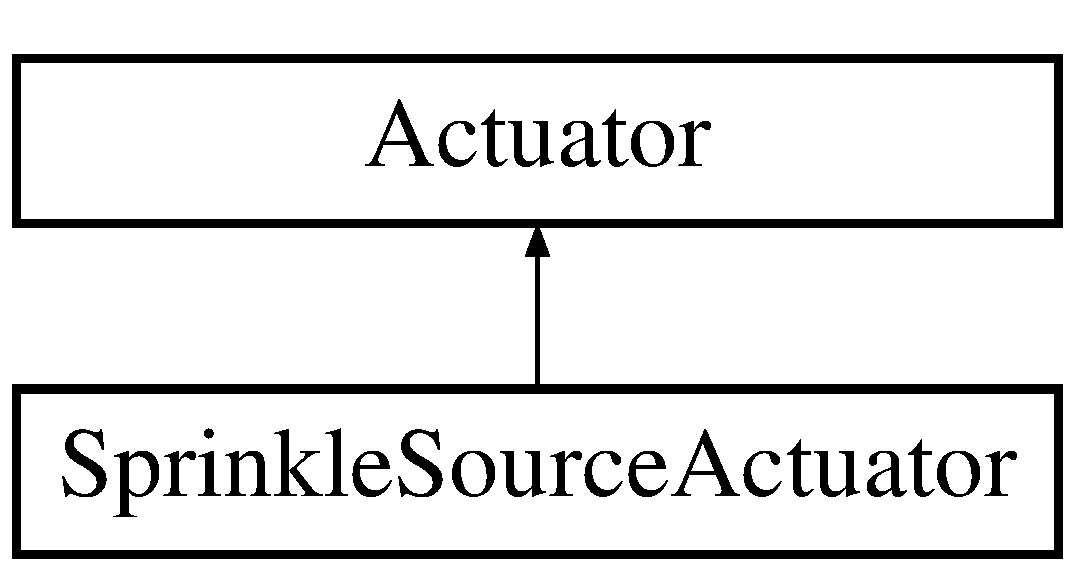
\includegraphics[height=2.000000cm]{classSprinkleSourceActuator}
\end{center}
\end{figure}
\subsection*{Public Member Functions}
\begin{DoxyCompactItemize}
\item 
\hyperlink{classSprinkleSourceActuator_ad5c37f4cec656b8c7709f26e11ecd7a1}{Sprinkle\-Source\-Actuator} (int id, \hyperlink{classSprinkleSource}{Sprinkle\-Source} $\ast$sprinkle\-Source)
\item 
virtual void \hyperlink{classSprinkleSourceActuator_ad61ef520615f3ad27964c9388da99825}{draw\-Label} ()
\item 
void \hyperlink{classSprinkleSourceActuator_a273206caefb1bfa72320f7b096a004ed}{set} (signed int value)
\item 
void \hyperlink{classSprinkleSourceActuator_a92ea18d960f132ec493d3b0400a0c504}{run} ()
\end{DoxyCompactItemize}
\subsection*{Public Attributes}
\begin{DoxyCompactItemize}
\item 
\hyperlink{classSprinkleSource}{Sprinkle\-Source} $\ast$ \hyperlink{classSprinkleSourceActuator_a796daa80fb757c0db169b92c13f8d836}{m\-\_\-sprinkle\-Source}
\end{DoxyCompactItemize}


\subsection{Detailed Description}
Produce \char`\"{}sprinkles\char`\"{} at a specific position, by controlling a sprinkle-\/source. 

\subsection{Constructor \& Destructor Documentation}
\hypertarget{classSprinkleSourceActuator_ad5c37f4cec656b8c7709f26e11ecd7a1}{\index{Sprinkle\-Source\-Actuator@{Sprinkle\-Source\-Actuator}!Sprinkle\-Source\-Actuator@{Sprinkle\-Source\-Actuator}}
\index{Sprinkle\-Source\-Actuator@{Sprinkle\-Source\-Actuator}!SprinkleSourceActuator@{Sprinkle\-Source\-Actuator}}
\subsubsection[{Sprinkle\-Source\-Actuator}]{\setlength{\rightskip}{0pt plus 5cm}Sprinkle\-Source\-Actuator\-::\-Sprinkle\-Source\-Actuator (
\begin{DoxyParamCaption}
\item[{int}]{id, }
\item[{{\bf Sprinkle\-Source} $\ast$}]{sprinkle\-Source}
\end{DoxyParamCaption}
)}}\label{classSprinkleSourceActuator_ad5c37f4cec656b8c7709f26e11ecd7a1}


\subsection{Member Function Documentation}
\hypertarget{classSprinkleSourceActuator_ad61ef520615f3ad27964c9388da99825}{\index{Sprinkle\-Source\-Actuator@{Sprinkle\-Source\-Actuator}!draw\-Label@{draw\-Label}}
\index{draw\-Label@{draw\-Label}!SprinkleSourceActuator@{Sprinkle\-Source\-Actuator}}
\subsubsection[{draw\-Label}]{\setlength{\rightskip}{0pt plus 5cm}void Sprinkle\-Source\-Actuator\-::draw\-Label (
\begin{DoxyParamCaption}
{}
\end{DoxyParamCaption}
)\hspace{0.3cm}{\ttfamily [virtual]}}}\label{classSprinkleSourceActuator_ad61ef520615f3ad27964c9388da99825}


Reimplemented from \hyperlink{classActuator_aaa39a438315ac34dbb1a4237bf70ff99}{Actuator}.

\hypertarget{classSprinkleSourceActuator_a92ea18d960f132ec493d3b0400a0c504}{\index{Sprinkle\-Source\-Actuator@{Sprinkle\-Source\-Actuator}!run@{run}}
\index{run@{run}!SprinkleSourceActuator@{Sprinkle\-Source\-Actuator}}
\subsubsection[{run}]{\setlength{\rightskip}{0pt plus 5cm}void Sprinkle\-Source\-Actuator\-::run (
\begin{DoxyParamCaption}
{}
\end{DoxyParamCaption}
)\hspace{0.3cm}{\ttfamily [virtual]}}}\label{classSprinkleSourceActuator_a92ea18d960f132ec493d3b0400a0c504}


Reimplemented from \hyperlink{classActuator_aabe48a4249a91a4cd1b964001fe754fc}{Actuator}.

\hypertarget{classSprinkleSourceActuator_a273206caefb1bfa72320f7b096a004ed}{\index{Sprinkle\-Source\-Actuator@{Sprinkle\-Source\-Actuator}!set@{set}}
\index{set@{set}!SprinkleSourceActuator@{Sprinkle\-Source\-Actuator}}
\subsubsection[{set}]{\setlength{\rightskip}{0pt plus 5cm}void Sprinkle\-Source\-Actuator\-::set (
\begin{DoxyParamCaption}
\item[{signed int}]{value}
\end{DoxyParamCaption}
)\hspace{0.3cm}{\ttfamily [virtual]}}}\label{classSprinkleSourceActuator_a273206caefb1bfa72320f7b096a004ed}


Reimplemented from \hyperlink{classActuator_a6281019cccd4034ab2cf7071defecf70}{Actuator}.



\subsection{Member Data Documentation}
\hypertarget{classSprinkleSourceActuator_a796daa80fb757c0db169b92c13f8d836}{\index{Sprinkle\-Source\-Actuator@{Sprinkle\-Source\-Actuator}!m\-\_\-sprinkle\-Source@{m\-\_\-sprinkle\-Source}}
\index{m\-\_\-sprinkle\-Source@{m\-\_\-sprinkle\-Source}!SprinkleSourceActuator@{Sprinkle\-Source\-Actuator}}
\subsubsection[{m\-\_\-sprinkle\-Source}]{\setlength{\rightskip}{0pt plus 5cm}{\bf Sprinkle\-Source}$\ast$ Sprinkle\-Source\-Actuator\-::m\-\_\-sprinkle\-Source}}\label{classSprinkleSourceActuator_a796daa80fb757c0db169b92c13f8d836}


The documentation for this class was generated from the following files\-:\begin{DoxyCompactItemize}
\item 
\hyperlink{Actuators_8h}{Actuators.\-h}\item 
\hyperlink{Actuators_8cpp}{Actuators.\-cpp}\end{DoxyCompactItemize}

\hypertarget{classStorage}{\section{Storage Class Reference}
\label{classStorage}\index{Storage@{Storage}}
}


Create an individual storage to sort planks into.  




{\ttfamily \#include $<$Storages.\-h$>$}

\subsection*{Public Member Functions}
\begin{DoxyCompactItemize}
\item 
\hyperlink{classStorage_a65c2cbe07917448e17db98e7a1661cea}{Storage} (b2\-Vec2 upper\-Left\-Corner, float32 width, float32 height, float32 wall\-Thickness, b2\-World $\ast$world)
\begin{DoxyCompactList}\small\item\em Construct a \hyperlink{classStorage}{Storage}. \end{DoxyCompactList}\item 
b2\-Prismatic\-Joint $\ast$ \hyperlink{classStorage_a1c5c79f11fa271b28e0ac22ea0649c40}{get\-Lift\-Joint} ()
\begin{DoxyCompactList}\small\item\em Return the lift\-Joint. \end{DoxyCompactList}\item 
b2\-Prismatic\-Joint $\ast$ \hyperlink{classStorage_a6e36f363dae08cf2f4b308b1e0a1e1bd}{get\-Stopper\-Joint} ()
\begin{DoxyCompactList}\small\item\em Return the stopper\-Joint. \end{DoxyCompactList}\item 
b2\-Fixture $\ast$ \hyperlink{classStorage_a585cdae218715a238dfc4277f875df60}{get\-Top\-Sensor\-Fixture} ()
\begin{DoxyCompactList}\small\item\em Return the top\-Sensor\-Fixture. \end{DoxyCompactList}\item 
b2\-Fixture $\ast$ \hyperlink{classStorage_ad22d8f7e6c28ba888bf7abd016e9ec38}{get\-Middle\-Sensor\-Fixture} ()
\begin{DoxyCompactList}\small\item\em Return the middle\-Sensor\-Fixture. \end{DoxyCompactList}\item 
b2\-Fixture $\ast$ \hyperlink{classStorage_a02014b1514942bedd63a7e2456982f39}{get\-Bottom\-Sensor\-Fixture} ()
\begin{DoxyCompactList}\small\item\em Return the bottom\-Sensor\-Fixture. \end{DoxyCompactList}\end{DoxyCompactItemize}
\subsection*{Public Attributes}
\begin{DoxyCompactItemize}
\item 
b2\-Body $\ast$ \hyperlink{classStorage_a3bae1d833350258742b94caca470e735}{m\-\_\-body\-Stopper}
\item 
b2\-Prismatic\-Joint $\ast$ \hyperlink{classStorage_a989c2bbe46e9874a4f4fed780a3d5de6}{m\-\_\-joint\-Lift}
\item 
b2\-Prismatic\-Joint $\ast$ \hyperlink{classStorage_ae96e6bf24e9d9c9788129bb6d87d10ab}{m\-\_\-joint\-Stopper}
\item 
b2\-Fixture $\ast$ \hyperlink{classStorage_afa862f61854f0960b41ae24b673b3980}{m\-\_\-fixture\-Top\-Sensor}
\item 
b2\-Fixture $\ast$ \hyperlink{classStorage_a27bcc4c94a7766c56f98ace7e2c3b662}{m\-\_\-fixture\-Middle\-Sensor}
\item 
b2\-Fixture $\ast$ \hyperlink{classStorage_afa76f1b21a27a64ef14d2360cc518bc3}{m\-\_\-fixture\-Bottom\-Sensor}
\end{DoxyCompactItemize}


\subsection{Detailed Description}
Create an individual storage to sort planks into. 

The Following line of code generates an instance of the Storage-\/class\-: 
\begin{DoxyCode}
\hyperlink{classStorage}{Storage}* storage = \textcolor{keyword}{new} \hyperlink{classStorage_a65c2cbe07917448e17db98e7a1661cea}{Storage}(b2Vec2(-40.0f,0.0f),9,5,0.5f,
      m\_world);
\end{DoxyCode}


Storage-\/instance + descriptive text\-:  

\subsection{Constructor \& Destructor Documentation}
\hypertarget{classStorage_a65c2cbe07917448e17db98e7a1661cea}{\index{Storage@{Storage}!Storage@{Storage}}
\index{Storage@{Storage}!Storage@{Storage}}
\subsubsection[{Storage}]{\setlength{\rightskip}{0pt plus 5cm}Storage\-::\-Storage (
\begin{DoxyParamCaption}
\item[{b2\-Vec2}]{upper\-Left\-Corner, }
\item[{float32}]{width, }
\item[{float32}]{height, }
\item[{float32}]{wall\-Thickness, }
\item[{b2\-World $\ast$}]{world}
\end{DoxyParamCaption}
)}}\label{classStorage_a65c2cbe07917448e17db98e7a1661cea}


Construct a \hyperlink{classStorage}{Storage}. 


\begin{DoxyParams}{Parameters}
{\em upper\-Left\-Corner} & The upper left corner of the storage. \\
\hline
{\em width} & The width of the storage. \\
\hline
{\em height} & The height of the storage. \\
\hline
{\em wall\-Thickness} & The thickness of the storages walls. \\
\hline
{\em world} & Pointer to world you want to create the storage in. \\
\hline
\end{DoxyParams}


\subsection{Member Function Documentation}
\hypertarget{classStorage_a02014b1514942bedd63a7e2456982f39}{\index{Storage@{Storage}!get\-Bottom\-Sensor\-Fixture@{get\-Bottom\-Sensor\-Fixture}}
\index{get\-Bottom\-Sensor\-Fixture@{get\-Bottom\-Sensor\-Fixture}!Storage@{Storage}}
\subsubsection[{get\-Bottom\-Sensor\-Fixture}]{\setlength{\rightskip}{0pt plus 5cm}b2\-Fixture$\ast$ Storage\-::get\-Bottom\-Sensor\-Fixture (
\begin{DoxyParamCaption}
{}
\end{DoxyParamCaption}
)\hspace{0.3cm}{\ttfamily [inline]}}}\label{classStorage_a02014b1514942bedd63a7e2456982f39}


Return the bottom\-Sensor\-Fixture. 

\hypertarget{classStorage_a1c5c79f11fa271b28e0ac22ea0649c40}{\index{Storage@{Storage}!get\-Lift\-Joint@{get\-Lift\-Joint}}
\index{get\-Lift\-Joint@{get\-Lift\-Joint}!Storage@{Storage}}
\subsubsection[{get\-Lift\-Joint}]{\setlength{\rightskip}{0pt plus 5cm}b2\-Prismatic\-Joint$\ast$ Storage\-::get\-Lift\-Joint (
\begin{DoxyParamCaption}
{}
\end{DoxyParamCaption}
)\hspace{0.3cm}{\ttfamily [inline]}}}\label{classStorage_a1c5c79f11fa271b28e0ac22ea0649c40}


Return the lift\-Joint. 

\hypertarget{classStorage_ad22d8f7e6c28ba888bf7abd016e9ec38}{\index{Storage@{Storage}!get\-Middle\-Sensor\-Fixture@{get\-Middle\-Sensor\-Fixture}}
\index{get\-Middle\-Sensor\-Fixture@{get\-Middle\-Sensor\-Fixture}!Storage@{Storage}}
\subsubsection[{get\-Middle\-Sensor\-Fixture}]{\setlength{\rightskip}{0pt plus 5cm}b2\-Fixture$\ast$ Storage\-::get\-Middle\-Sensor\-Fixture (
\begin{DoxyParamCaption}
{}
\end{DoxyParamCaption}
)\hspace{0.3cm}{\ttfamily [inline]}}}\label{classStorage_ad22d8f7e6c28ba888bf7abd016e9ec38}


Return the middle\-Sensor\-Fixture. 

\hypertarget{classStorage_a6e36f363dae08cf2f4b308b1e0a1e1bd}{\index{Storage@{Storage}!get\-Stopper\-Joint@{get\-Stopper\-Joint}}
\index{get\-Stopper\-Joint@{get\-Stopper\-Joint}!Storage@{Storage}}
\subsubsection[{get\-Stopper\-Joint}]{\setlength{\rightskip}{0pt plus 5cm}b2\-Prismatic\-Joint$\ast$ Storage\-::get\-Stopper\-Joint (
\begin{DoxyParamCaption}
{}
\end{DoxyParamCaption}
)\hspace{0.3cm}{\ttfamily [inline]}}}\label{classStorage_a6e36f363dae08cf2f4b308b1e0a1e1bd}


Return the stopper\-Joint. 

\hypertarget{classStorage_a585cdae218715a238dfc4277f875df60}{\index{Storage@{Storage}!get\-Top\-Sensor\-Fixture@{get\-Top\-Sensor\-Fixture}}
\index{get\-Top\-Sensor\-Fixture@{get\-Top\-Sensor\-Fixture}!Storage@{Storage}}
\subsubsection[{get\-Top\-Sensor\-Fixture}]{\setlength{\rightskip}{0pt plus 5cm}b2\-Fixture$\ast$ Storage\-::get\-Top\-Sensor\-Fixture (
\begin{DoxyParamCaption}
{}
\end{DoxyParamCaption}
)\hspace{0.3cm}{\ttfamily [inline]}}}\label{classStorage_a585cdae218715a238dfc4277f875df60}


Return the top\-Sensor\-Fixture. 



\subsection{Member Data Documentation}
\hypertarget{classStorage_a3bae1d833350258742b94caca470e735}{\index{Storage@{Storage}!m\-\_\-body\-Stopper@{m\-\_\-body\-Stopper}}
\index{m\-\_\-body\-Stopper@{m\-\_\-body\-Stopper}!Storage@{Storage}}
\subsubsection[{m\-\_\-body\-Stopper}]{\setlength{\rightskip}{0pt plus 5cm}b2\-Body$\ast$ Storage\-::m\-\_\-body\-Stopper}}\label{classStorage_a3bae1d833350258742b94caca470e735}
\hypertarget{classStorage_afa76f1b21a27a64ef14d2360cc518bc3}{\index{Storage@{Storage}!m\-\_\-fixture\-Bottom\-Sensor@{m\-\_\-fixture\-Bottom\-Sensor}}
\index{m\-\_\-fixture\-Bottom\-Sensor@{m\-\_\-fixture\-Bottom\-Sensor}!Storage@{Storage}}
\subsubsection[{m\-\_\-fixture\-Bottom\-Sensor}]{\setlength{\rightskip}{0pt plus 5cm}b2\-Fixture$\ast$ Storage\-::m\-\_\-fixture\-Bottom\-Sensor}}\label{classStorage_afa76f1b21a27a64ef14d2360cc518bc3}
\hypertarget{classStorage_a27bcc4c94a7766c56f98ace7e2c3b662}{\index{Storage@{Storage}!m\-\_\-fixture\-Middle\-Sensor@{m\-\_\-fixture\-Middle\-Sensor}}
\index{m\-\_\-fixture\-Middle\-Sensor@{m\-\_\-fixture\-Middle\-Sensor}!Storage@{Storage}}
\subsubsection[{m\-\_\-fixture\-Middle\-Sensor}]{\setlength{\rightskip}{0pt plus 5cm}b2\-Fixture$\ast$ Storage\-::m\-\_\-fixture\-Middle\-Sensor}}\label{classStorage_a27bcc4c94a7766c56f98ace7e2c3b662}
\hypertarget{classStorage_afa862f61854f0960b41ae24b673b3980}{\index{Storage@{Storage}!m\-\_\-fixture\-Top\-Sensor@{m\-\_\-fixture\-Top\-Sensor}}
\index{m\-\_\-fixture\-Top\-Sensor@{m\-\_\-fixture\-Top\-Sensor}!Storage@{Storage}}
\subsubsection[{m\-\_\-fixture\-Top\-Sensor}]{\setlength{\rightskip}{0pt plus 5cm}b2\-Fixture$\ast$ Storage\-::m\-\_\-fixture\-Top\-Sensor}}\label{classStorage_afa862f61854f0960b41ae24b673b3980}
\hypertarget{classStorage_a989c2bbe46e9874a4f4fed780a3d5de6}{\index{Storage@{Storage}!m\-\_\-joint\-Lift@{m\-\_\-joint\-Lift}}
\index{m\-\_\-joint\-Lift@{m\-\_\-joint\-Lift}!Storage@{Storage}}
\subsubsection[{m\-\_\-joint\-Lift}]{\setlength{\rightskip}{0pt plus 5cm}b2\-Prismatic\-Joint$\ast$ Storage\-::m\-\_\-joint\-Lift}}\label{classStorage_a989c2bbe46e9874a4f4fed780a3d5de6}
\hypertarget{classStorage_ae96e6bf24e9d9c9788129bb6d87d10ab}{\index{Storage@{Storage}!m\-\_\-joint\-Stopper@{m\-\_\-joint\-Stopper}}
\index{m\-\_\-joint\-Stopper@{m\-\_\-joint\-Stopper}!Storage@{Storage}}
\subsubsection[{m\-\_\-joint\-Stopper}]{\setlength{\rightskip}{0pt plus 5cm}b2\-Prismatic\-Joint$\ast$ Storage\-::m\-\_\-joint\-Stopper}}\label{classStorage_ae96e6bf24e9d9c9788129bb6d87d10ab}


The documentation for this class was generated from the following files\-:\begin{DoxyCompactItemize}
\item 
\hyperlink{Storages_8h}{Storages.\-h}\item 
\hyperlink{Storages_8cpp}{Storages.\-cpp}\end{DoxyCompactItemize}

\hypertarget{classStorageArea}{\section{Storage\-Area Class Reference}
\label{classStorageArea}\index{Storage\-Area@{Storage\-Area}}
}


Create an arbitrary number of storages side-\/by-\/side to sort planks into.  




{\ttfamily \#include $<$Storages.\-h$>$}

\subsection*{Public Member Functions}
\begin{DoxyCompactItemize}
\item 
\hyperlink{classStorageArea_a4a5f9f5686f968f55810b61ad7842650}{Storage\-Area} (int number\-Of\-Storages, b2\-Vec2 upper\-Left\-Corner, float32 width, float32 height, float32 wall\-Thickness, b2\-World $\ast$world)
\begin{DoxyCompactList}\small\item\em Construct an arbitrary number of storages side-\/by-\/side. \end{DoxyCompactList}\item 
b2\-Prismatic\-Joint $\ast$ \hyperlink{classStorageArea_a0885600a2b998f164acdc93f88d384d0}{get\-Lift\-Joint} (int i)
\item 
b2\-Prismatic\-Joint $\ast$ \hyperlink{classStorageArea_aea535b0b0abe0235582239ab0851b73e}{get\-Stopper\-Joint} (int i)
\item 
b2\-Fixture $\ast$ \hyperlink{classStorageArea_a1c797933bfbf9e3aaef52190630277e4}{get\-Top\-Sensor\-Fixture} (int i)
\item 
b2\-Fixture $\ast$ \hyperlink{classStorageArea_a2ea9264e9f7243ca6f2e66e99e5d13a8}{get\-Middle\-Sensor\-Fixture} (int i)
\item 
b2\-Fixture $\ast$ \hyperlink{classStorageArea_a3c2ddd3fe7e2f26b9be4ec9564257f5d}{get\-Bottom\-Sensor\-Fixture} (int i)
\end{DoxyCompactItemize}
\subsection*{Public Attributes}
\begin{DoxyCompactItemize}
\item 
vector$<$ \hyperlink{classStorage}{Storage} $\ast$ $>$ \hyperlink{classStorageArea_ab5c3b86896768610f1b558126bf0df71}{m\-\_\-storage}
\begin{DoxyCompactList}\small\item\em Vector that contains pointers to the individual storages. \end{DoxyCompactList}\end{DoxyCompactItemize}


\subsection{Detailed Description}
Create an arbitrary number of storages side-\/by-\/side to sort planks into. 

The Following line of code generates the storage area in the image below. 
\begin{DoxyCode}
\hyperlink{classStorageArea}{StorageArea}* storageArea0 = \textcolor{keyword}{new} \hyperlink{classStorageArea_a4a5f9f5686f968f55810b61ad7842650}{StorageArea}(3,b2Vec2(-40.
      0f,0.0f),9,5,0.5f,m\_world);
\end{DoxyCode}


Instance of \hyperlink{classStorageArea}{Storage\-Area} + descriptive text\-:  

\subsection{Constructor \& Destructor Documentation}
\hypertarget{classStorageArea_a4a5f9f5686f968f55810b61ad7842650}{\index{Storage\-Area@{Storage\-Area}!Storage\-Area@{Storage\-Area}}
\index{Storage\-Area@{Storage\-Area}!StorageArea@{Storage\-Area}}
\subsubsection[{Storage\-Area}]{\setlength{\rightskip}{0pt plus 5cm}Storage\-Area\-::\-Storage\-Area (
\begin{DoxyParamCaption}
\item[{int}]{number\-Of\-Storages, }
\item[{b2\-Vec2}]{upper\-Left\-Corner, }
\item[{float32}]{width, }
\item[{float32}]{height, }
\item[{float32}]{wall\-Thickness, }
\item[{b2\-World $\ast$}]{world}
\end{DoxyParamCaption}
)}}\label{classStorageArea_a4a5f9f5686f968f55810b61ad7842650}


Construct an arbitrary number of storages side-\/by-\/side. 


\begin{DoxyParams}{Parameters}
{\em number\-Of\-Storages} & The number of storages. \\
\hline
{\em upper\-Left\-Corner} & Positioin of the upper left corner of the first storage. \\
\hline
{\em width} & The width of an individual storage. \\
\hline
{\em height} & The height of an individual storage. \\
\hline
{\em wall\-Thickness} & The wall-\/thickness of an individual storage. \\
\hline
{\em world} & Pointer to the world you want to create the storage-\/area in. \\
\hline
\end{DoxyParams}


\subsection{Member Function Documentation}
\hypertarget{classStorageArea_a3c2ddd3fe7e2f26b9be4ec9564257f5d}{\index{Storage\-Area@{Storage\-Area}!get\-Bottom\-Sensor\-Fixture@{get\-Bottom\-Sensor\-Fixture}}
\index{get\-Bottom\-Sensor\-Fixture@{get\-Bottom\-Sensor\-Fixture}!StorageArea@{Storage\-Area}}
\subsubsection[{get\-Bottom\-Sensor\-Fixture}]{\setlength{\rightskip}{0pt plus 5cm}b2\-Fixture $\ast$ Storage\-Area\-::get\-Bottom\-Sensor\-Fixture (
\begin{DoxyParamCaption}
\item[{int}]{i}
\end{DoxyParamCaption}
)}}\label{classStorageArea_a3c2ddd3fe7e2f26b9be4ec9564257f5d}
\hypertarget{classStorageArea_a0885600a2b998f164acdc93f88d384d0}{\index{Storage\-Area@{Storage\-Area}!get\-Lift\-Joint@{get\-Lift\-Joint}}
\index{get\-Lift\-Joint@{get\-Lift\-Joint}!StorageArea@{Storage\-Area}}
\subsubsection[{get\-Lift\-Joint}]{\setlength{\rightskip}{0pt plus 5cm}b2\-Prismatic\-Joint $\ast$ Storage\-Area\-::get\-Lift\-Joint (
\begin{DoxyParamCaption}
\item[{int}]{i}
\end{DoxyParamCaption}
)}}\label{classStorageArea_a0885600a2b998f164acdc93f88d384d0}
\hypertarget{classStorageArea_a2ea9264e9f7243ca6f2e66e99e5d13a8}{\index{Storage\-Area@{Storage\-Area}!get\-Middle\-Sensor\-Fixture@{get\-Middle\-Sensor\-Fixture}}
\index{get\-Middle\-Sensor\-Fixture@{get\-Middle\-Sensor\-Fixture}!StorageArea@{Storage\-Area}}
\subsubsection[{get\-Middle\-Sensor\-Fixture}]{\setlength{\rightskip}{0pt plus 5cm}b2\-Fixture $\ast$ Storage\-Area\-::get\-Middle\-Sensor\-Fixture (
\begin{DoxyParamCaption}
\item[{int}]{i}
\end{DoxyParamCaption}
)}}\label{classStorageArea_a2ea9264e9f7243ca6f2e66e99e5d13a8}
\hypertarget{classStorageArea_aea535b0b0abe0235582239ab0851b73e}{\index{Storage\-Area@{Storage\-Area}!get\-Stopper\-Joint@{get\-Stopper\-Joint}}
\index{get\-Stopper\-Joint@{get\-Stopper\-Joint}!StorageArea@{Storage\-Area}}
\subsubsection[{get\-Stopper\-Joint}]{\setlength{\rightskip}{0pt plus 5cm}b2\-Prismatic\-Joint $\ast$ Storage\-Area\-::get\-Stopper\-Joint (
\begin{DoxyParamCaption}
\item[{int}]{i}
\end{DoxyParamCaption}
)}}\label{classStorageArea_aea535b0b0abe0235582239ab0851b73e}
\hypertarget{classStorageArea_a1c797933bfbf9e3aaef52190630277e4}{\index{Storage\-Area@{Storage\-Area}!get\-Top\-Sensor\-Fixture@{get\-Top\-Sensor\-Fixture}}
\index{get\-Top\-Sensor\-Fixture@{get\-Top\-Sensor\-Fixture}!StorageArea@{Storage\-Area}}
\subsubsection[{get\-Top\-Sensor\-Fixture}]{\setlength{\rightskip}{0pt plus 5cm}b2\-Fixture $\ast$ Storage\-Area\-::get\-Top\-Sensor\-Fixture (
\begin{DoxyParamCaption}
\item[{int}]{i}
\end{DoxyParamCaption}
)}}\label{classStorageArea_a1c797933bfbf9e3aaef52190630277e4}


\subsection{Member Data Documentation}
\hypertarget{classStorageArea_ab5c3b86896768610f1b558126bf0df71}{\index{Storage\-Area@{Storage\-Area}!m\-\_\-storage@{m\-\_\-storage}}
\index{m\-\_\-storage@{m\-\_\-storage}!StorageArea@{Storage\-Area}}
\subsubsection[{m\-\_\-storage}]{\setlength{\rightskip}{0pt plus 5cm}vector$<${\bf Storage}$\ast$$>$ Storage\-Area\-::m\-\_\-storage}}\label{classStorageArea_ab5c3b86896768610f1b558126bf0df71}


Vector that contains pointers to the individual storages. 



The documentation for this class was generated from the following files\-:\begin{DoxyCompactItemize}
\item 
\hyperlink{Storages_8h}{Storages.\-h}\item 
\hyperlink{Storages_8cpp}{Storages.\-cpp}\end{DoxyCompactItemize}

\hypertarget{classStorageLiftUserData}{\section{Storage\-Lift\-User\-Data Class Reference}
\label{classStorageLiftUserData}\index{Storage\-Lift\-User\-Data@{Storage\-Lift\-User\-Data}}
}


Identify a b2\-Fixture as a storage-\/lift.  




{\ttfamily \#include $<$User\-Data.\-h$>$}

Inheritance diagram for Storage\-Lift\-User\-Data\-:\begin{figure}[H]
\begin{center}
\leavevmode
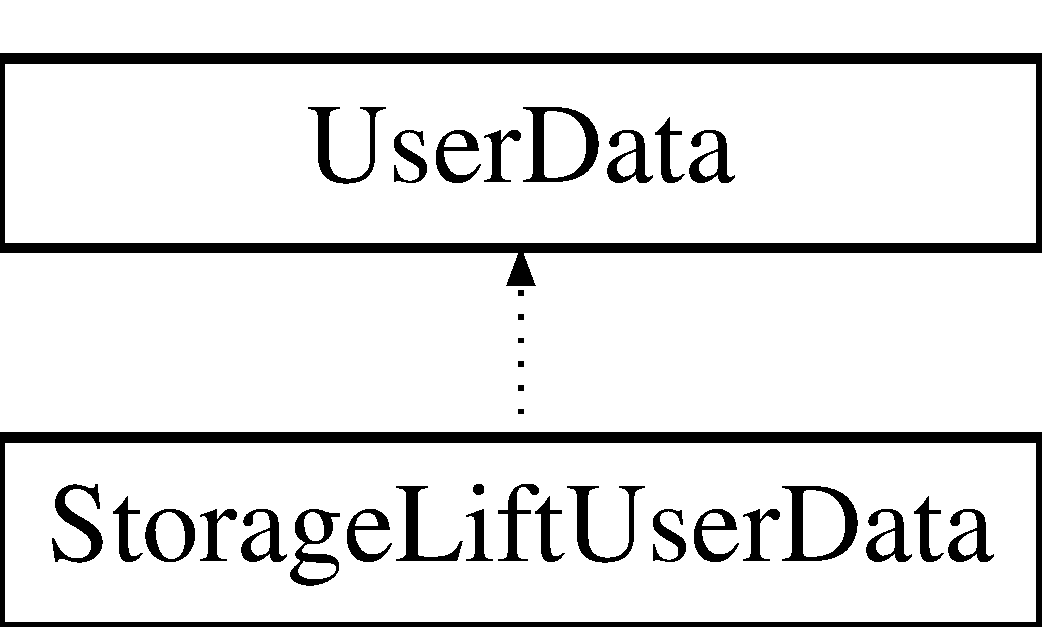
\includegraphics[height=2.000000cm]{classStorageLiftUserData}
\end{center}
\end{figure}
\subsection*{Public Member Functions}
\begin{DoxyCompactItemize}
\item 
\hyperlink{classStorageLiftUserData_a51fb52d638cc97778302fa4aeff98fb1}{Storage\-Lift\-User\-Data} ()
\end{DoxyCompactItemize}
\subsection*{Additional Inherited Members}


\subsection{Detailed Description}
Identify a b2\-Fixture as a storage-\/lift. 

Each storage-\/lifts b2\-Fixture points to an instance of this class. 

\subsection{Constructor \& Destructor Documentation}
\hypertarget{classStorageLiftUserData_a51fb52d638cc97778302fa4aeff98fb1}{\index{Storage\-Lift\-User\-Data@{Storage\-Lift\-User\-Data}!Storage\-Lift\-User\-Data@{Storage\-Lift\-User\-Data}}
\index{Storage\-Lift\-User\-Data@{Storage\-Lift\-User\-Data}!StorageLiftUserData@{Storage\-Lift\-User\-Data}}
\subsubsection[{Storage\-Lift\-User\-Data}]{\setlength{\rightskip}{0pt plus 5cm}Storage\-Lift\-User\-Data\-::\-Storage\-Lift\-User\-Data (
\begin{DoxyParamCaption}
{}
\end{DoxyParamCaption}
)\hspace{0.3cm}{\ttfamily [inline]}}}\label{classStorageLiftUserData_a51fb52d638cc97778302fa4aeff98fb1}


The documentation for this class was generated from the following file\-:\begin{DoxyCompactItemize}
\item 
\hyperlink{UserData_8h}{User\-Data.\-h}\end{DoxyCompactItemize}

\hypertarget{classUserData}{\section{User\-Data Class Reference}
\label{classUserData}\index{User\-Data@{User\-Data}}
}


The archtypical userdata-\/class which other userdata-\/classes inherit from.  




{\ttfamily \#include $<$User\-Data.\-h$>$}

Inheritance diagram for User\-Data\-:\begin{figure}[H]
\begin{center}
\leavevmode
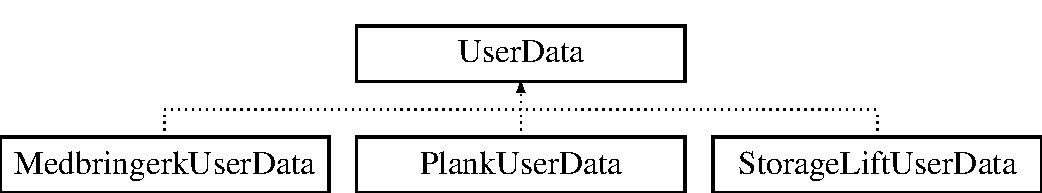
\includegraphics[height=2.000000cm]{classUserData}
\end{center}
\end{figure}
\subsection*{Public Member Functions}
\begin{DoxyCompactItemize}
\item 
\hyperlink{classUserData_a1d4f7b61ec5dd67bbd4e03efd4f85ce8}{User\-Data} ()
\end{DoxyCompactItemize}
\subsection*{Public Attributes}
\begin{DoxyCompactItemize}
\item 
\hyperlink{UserData_8h_a137995e5213a16d462ac7f64935fea34}{t\-\_\-user\-Data\-Type} \hyperlink{classUserData_acb084482d371d842c4ca1c6fc57f737d}{m\-\_\-type}
\end{DoxyCompactItemize}


\subsection{Detailed Description}
The archtypical userdata-\/class which other userdata-\/classes inherit from. 

These common features makes handling user-\/data much simpler. 

\subsection{Constructor \& Destructor Documentation}
\hypertarget{classUserData_a1d4f7b61ec5dd67bbd4e03efd4f85ce8}{\index{User\-Data@{User\-Data}!User\-Data@{User\-Data}}
\index{User\-Data@{User\-Data}!UserData@{User\-Data}}
\subsubsection[{User\-Data}]{\setlength{\rightskip}{0pt plus 5cm}User\-Data\-::\-User\-Data (
\begin{DoxyParamCaption}
{}
\end{DoxyParamCaption}
)\hspace{0.3cm}{\ttfamily [inline]}}}\label{classUserData_a1d4f7b61ec5dd67bbd4e03efd4f85ce8}


\subsection{Member Data Documentation}
\hypertarget{classUserData_acb084482d371d842c4ca1c6fc57f737d}{\index{User\-Data@{User\-Data}!m\-\_\-type@{m\-\_\-type}}
\index{m\-\_\-type@{m\-\_\-type}!UserData@{User\-Data}}
\subsubsection[{m\-\_\-type}]{\setlength{\rightskip}{0pt plus 5cm}{\bf t\-\_\-user\-Data\-Type} User\-Data\-::m\-\_\-type}}\label{classUserData_acb084482d371d842c4ca1c6fc57f737d}


The documentation for this class was generated from the following file\-:\begin{DoxyCompactItemize}
\item 
\hyperlink{UserData_8h}{User\-Data.\-h}\end{DoxyCompactItemize}

\hypertarget{classWheel}{\section{Wheel Class Reference}
\label{classWheel}\index{Wheel@{Wheel}}
}


The conveyors wheels.  




{\ttfamily \#include $<$Conveyor.\-h$>$}

\subsection*{Public Member Functions}
\begin{DoxyCompactItemize}
\item 
\hyperlink{classWheel_a087a6aff8ca3fd0ac8b4fdc3420dcfdd}{Wheel} (b2\-Vec2 p, float32 r, int cm\-Bits, b2\-World $\ast$world)
\item 
void \hyperlink{classWheel_a30373a17455666b38eeaf37a03dbc615}{set\-Speed} (float32 speed)
\item 
void \hyperlink{classWheel_acaa5238a23eab267cdd81f7b58330ad5}{run} ()
\item 
b2\-Body $\ast$ \hyperlink{classWheel_a7b245511bdc543bcc9f99cdd7275e600}{get\-Body} ()
\end{DoxyCompactItemize}
\subsection*{Private Attributes}
\begin{DoxyCompactItemize}
\item 
b2\-Body $\ast$ \hyperlink{classWheel_a025dd350776aa44dee750864bb9918f2}{m\-\_\-body}
\item 
float32 \hyperlink{classWheel_afff232bc89f91dfcf8a15be2a7af0307}{m\-\_\-speed}
\end{DoxyCompactItemize}


\subsection{Detailed Description}
The conveyors wheels. 

\subsection{Constructor \& Destructor Documentation}
\hypertarget{classWheel_a087a6aff8ca3fd0ac8b4fdc3420dcfdd}{\index{Wheel@{Wheel}!Wheel@{Wheel}}
\index{Wheel@{Wheel}!Wheel@{Wheel}}
\subsubsection[{Wheel}]{\setlength{\rightskip}{0pt plus 5cm}Wheel\-::\-Wheel (
\begin{DoxyParamCaption}
\item[{b2\-Vec2}]{p, }
\item[{float32}]{r, }
\item[{int}]{cm\-Bits, }
\item[{b2\-World $\ast$}]{world}
\end{DoxyParamCaption}
)}}\label{classWheel_a087a6aff8ca3fd0ac8b4fdc3420dcfdd}


\subsection{Member Function Documentation}
\hypertarget{classWheel_a7b245511bdc543bcc9f99cdd7275e600}{\index{Wheel@{Wheel}!get\-Body@{get\-Body}}
\index{get\-Body@{get\-Body}!Wheel@{Wheel}}
\subsubsection[{get\-Body}]{\setlength{\rightskip}{0pt plus 5cm}b2\-Body$\ast$ Wheel\-::get\-Body (
\begin{DoxyParamCaption}
{}
\end{DoxyParamCaption}
)\hspace{0.3cm}{\ttfamily [inline]}}}\label{classWheel_a7b245511bdc543bcc9f99cdd7275e600}
\hypertarget{classWheel_acaa5238a23eab267cdd81f7b58330ad5}{\index{Wheel@{Wheel}!run@{run}}
\index{run@{run}!Wheel@{Wheel}}
\subsubsection[{run}]{\setlength{\rightskip}{0pt plus 5cm}void Wheel\-::run (
\begin{DoxyParamCaption}
{}
\end{DoxyParamCaption}
)}}\label{classWheel_acaa5238a23eab267cdd81f7b58330ad5}
\hypertarget{classWheel_a30373a17455666b38eeaf37a03dbc615}{\index{Wheel@{Wheel}!set\-Speed@{set\-Speed}}
\index{set\-Speed@{set\-Speed}!Wheel@{Wheel}}
\subsubsection[{set\-Speed}]{\setlength{\rightskip}{0pt plus 5cm}void Wheel\-::set\-Speed (
\begin{DoxyParamCaption}
\item[{float32}]{speed}
\end{DoxyParamCaption}
)\hspace{0.3cm}{\ttfamily [inline]}}}\label{classWheel_a30373a17455666b38eeaf37a03dbc615}


\subsection{Member Data Documentation}
\hypertarget{classWheel_a025dd350776aa44dee750864bb9918f2}{\index{Wheel@{Wheel}!m\-\_\-body@{m\-\_\-body}}
\index{m\-\_\-body@{m\-\_\-body}!Wheel@{Wheel}}
\subsubsection[{m\-\_\-body}]{\setlength{\rightskip}{0pt plus 5cm}b2\-Body$\ast$ Wheel\-::m\-\_\-body\hspace{0.3cm}{\ttfamily [private]}}}\label{classWheel_a025dd350776aa44dee750864bb9918f2}
\hypertarget{classWheel_afff232bc89f91dfcf8a15be2a7af0307}{\index{Wheel@{Wheel}!m\-\_\-speed@{m\-\_\-speed}}
\index{m\-\_\-speed@{m\-\_\-speed}!Wheel@{Wheel}}
\subsubsection[{m\-\_\-speed}]{\setlength{\rightskip}{0pt plus 5cm}float32 Wheel\-::m\-\_\-speed\hspace{0.3cm}{\ttfamily [private]}}}\label{classWheel_afff232bc89f91dfcf8a15be2a7af0307}


The documentation for this class was generated from the following files\-:\begin{DoxyCompactItemize}
\item 
\hyperlink{Conveyor_8h}{Conveyor.\-h}\item 
\hyperlink{Conveyor_8cpp}{Conveyor.\-cpp}\end{DoxyCompactItemize}

\chapter{File Documentation}
\hypertarget{Actuators_8cpp}{\section{Actuators.\-cpp File Reference}
\label{Actuators_8cpp}\index{Actuators.\-cpp@{Actuators.\-cpp}}
}
{\ttfamily \#include \char`\"{}Actuators.\-h\char`\"{}}\\*

\hypertarget{Actuators_8h}{\section{Actuators.\-h File Reference}
\label{Actuators_8h}\index{Actuators.\-h@{Actuators.\-h}}
}


Contains actuator-\/hierarchy and actuator-\/set.  


{\ttfamily \#include $<$vector$>$}\\*
{\ttfamily \#include $<$string$>$}\\*
{\ttfamily \#include $<$sstream$>$}\\*
{\ttfamily \#include $<$boost/lexical\-\_\-cast.\-hpp$>$}\\*
{\ttfamily \#include \char`\"{}Text.\-h\char`\"{}}\\*
{\ttfamily \#include \char`\"{}Conveyor.\-h\char`\"{}}\\*
{\ttfamily \#include \char`\"{}Sensors.\-h\char`\"{}}\\*
{\ttfamily \#include \char`\"{}Package.\-h\char`\"{}}\\*
\subsection*{Classes}
\begin{DoxyCompactItemize}
\item 
class \hyperlink{classActuator}{Actuator}
\begin{DoxyCompactList}\small\item\em Abstract class from which other actuator-\/classes inherit. \end{DoxyCompactList}\item 
class \hyperlink{classConveyorActuator}{Conveyor\-Actuator}
\begin{DoxyCompactList}\small\item\em Abstact class from which conveyor-\/actuators inherit. \end{DoxyCompactList}\item 
class \hyperlink{classConveyorActuatorBinary}{Conveyor\-Actuator\-Binary}
\begin{DoxyCompactList}\small\item\em Turn a conveyor O\-N or O\-F\-F. \end{DoxyCompactList}\item 
class \hyperlink{classConveyorActuatorStep}{Conveyor\-Actuator\-Step}
\begin{DoxyCompactList}\small\item\em Run a conveyor an arbitrary number of steps. \end{DoxyCompactList}\item 
class \hyperlink{classJointActuatorPrismaticBinary}{Joint\-Actuator\-Prismatic\-Binary}
\begin{DoxyCompactList}\small\item\em Switch a prismatic joint between the two extremal states. \end{DoxyCompactList}\item 
class \hyperlink{classJointActuatorPrismaticRange}{Joint\-Actuator\-Prismatic\-Range}
\begin{DoxyCompactList}\small\item\em Run a prismatic joint at an arbitrary constant speed. \end{DoxyCompactList}\item 
class \hyperlink{classJointActuatorPrismaticStep}{Joint\-Actuator\-Prismatic\-Step}
\begin{DoxyCompactList}\small\item\em Run a prismatic joint an arbitrary number of steps. \end{DoxyCompactList}\item 
class \hyperlink{classJointActuatorRevoluteStep}{Joint\-Actuator\-Revolute\-Step}
\begin{DoxyCompactList}\small\item\em Turn a revolute joint an arbitrary angle. \end{DoxyCompactList}\item 
class \hyperlink{classPackageSourceActuator}{Package\-Source\-Actuator}
\begin{DoxyCompactList}\small\item\em Produce packages at a specific position, by controlling a package-\/source. \end{DoxyCompactList}\item 
class \hyperlink{classSprinkleSourceActuator}{Sprinkle\-Source\-Actuator}
\begin{DoxyCompactList}\small\item\em Produce \char`\"{}sprinkles\char`\"{} at a specific position, by controlling a sprinkle-\/source. \end{DoxyCompactList}\item 
class \hyperlink{classActuatorSet}{Actuator\-Set}
\begin{DoxyCompactList}\small\item\em Draw actuator-\/labels, run actuators and change the state of actuators by id. \end{DoxyCompactList}\end{DoxyCompactItemize}


\subsection{Detailed Description}
Contains actuator-\/hierarchy and actuator-\/set. \begin{DoxyAuthor}{Author}
Roy Kollen Svendsen 
\end{DoxyAuthor}

\hypertarget{CommandSequenceInterpreter_8cpp}{\section{Command\-Sequence\-Interpreter.\-cpp File Reference}
\label{CommandSequenceInterpreter_8cpp}\index{Command\-Sequence\-Interpreter.\-cpp@{Command\-Sequence\-Interpreter.\-cpp}}
}
{\ttfamily \#include \char`\"{}Command\-Sequence\-Interpreter.\-h\char`\"{}}\\*

\hypertarget{CommandSequenceInterpreter_8h}{\section{Command\-Sequence\-Interpreter.\-h File Reference}
\label{CommandSequenceInterpreter_8h}\index{Command\-Sequence\-Interpreter.\-h@{Command\-Sequence\-Interpreter.\-h}}
}


Contains the Command\-Sequance\-Interpreter-\/class.  


{\ttfamily \#include $<$string$>$}\\*
{\ttfamily \#include $<$sstream$>$}\\*
{\ttfamily \#include $<$vector$>$}\\*
{\ttfamily \#include \char`\"{}Actuators.\-h\char`\"{}}\\*
{\ttfamily \#include \char`\"{}Sensors.\-h\char`\"{}}\\*
\subsection*{Classes}
\begin{DoxyCompactItemize}
\item 
class \hyperlink{classCommandSequenceInterpreter}{Command\-Sequence\-Interpreter}
\begin{DoxyCompactList}\small\item\em Use keyboard-\/ or terminal-\/input to control the actuator-\/ and sensor-\/sets. \end{DoxyCompactList}\end{DoxyCompactItemize}


\subsection{Detailed Description}
Contains the Command\-Sequance\-Interpreter-\/class. \begin{DoxyAuthor}{Author}
Roy Kollen Svendsen 
\end{DoxyAuthor}

\hypertarget{Communicator_8cpp}{\section{Communicator.\-cpp File Reference}
\label{Communicator_8cpp}\index{Communicator.\-cpp@{Communicator.\-cpp}}
}
{\ttfamily \#include \char`\"{}Communicator.\-h\char`\"{}}\\*

\hypertarget{Communicator_8h}{\section{Communicator.\-h File Reference}
\label{Communicator_8h}\index{Communicator.\-h@{Communicator.\-h}}
}


Contains the Communicator-\/class.  


{\ttfamily \#include $<$iostream$>$}\\*
{\ttfamily \#include $<$string.\-h$>$}\\*
{\ttfamily \#include $<$sstream$>$}\\*
{\ttfamily \#include $<$boost/system/error\-\_\-code.\-hpp$>$}\\*
{\ttfamily \#include $<$boost/asio.\-hpp$>$}\\*
{\ttfamily \#include $<$boost/thread.\-hpp$>$}\\*
{\ttfamily \#include $<$exception$>$}\\*
{\ttfamily \#include $<$deque$>$}\\*
{\ttfamily \#include $<$stdlib.\-h$>$}\\*
{\ttfamily \#include $<$stdio.\-h$>$}\\*
{\ttfamily \#include $<$stdarg.\-h$>$}\\*
\subsection*{Classes}
\begin{DoxyCompactItemize}
\item 
class \hyperlink{classCommunicator}{Communicator}
\begin{DoxyCompactList}\small\item\em Read frowm and write to an arbitrary serial-\/port. \end{DoxyCompactList}\end{DoxyCompactItemize}


\subsection{Detailed Description}
Contains the Communicator-\/class. \begin{DoxyAuthor}{Author}
Roy Kollen Svendsen 
\end{DoxyAuthor}

\hypertarget{Conveyor_8cpp}{\section{Conveyor.\-cpp File Reference}
\label{Conveyor_8cpp}\index{Conveyor.\-cpp@{Conveyor.\-cpp}}
}
{\ttfamily \#include \char`\"{}Conveyor.\-h\char`\"{}}\\*

\hypertarget{Conveyor_8h}{\section{Conveyor.\-h File Reference}
\label{Conveyor_8h}\index{Conveyor.\-h@{Conveyor.\-h}}
}


Contains the Conveyor-\/class and the classes needed to build it.  


{\ttfamily \#include $<$vector$>$}\\*
{\ttfamily \#include \char`\"{}Sensors.\-h\char`\"{}}\\*
\subsection*{Classes}
\begin{DoxyCompactItemize}
\item 
class \hyperlink{classWheel}{Wheel}
\begin{DoxyCompactList}\small\item\em The conveyors wheels. \end{DoxyCompactList}\item 
class \hyperlink{classBeam}{Beam}
\begin{DoxyCompactList}\small\item\em The beam which the wheels are attached to and which the belt runs along. \end{DoxyCompactList}\item 
class \hyperlink{classConveyorBelt}{Conveyor\-Belt}
\begin{DoxyCompactList}\small\item\em The conveyorbelt. \end{DoxyCompactList}\item 
class \hyperlink{classConveyorBeltShield}{Conveyor\-Belt\-Shield}
\begin{DoxyCompactList}\small\item\em Hinder the conveyorbelt in falling off. \end{DoxyCompactList}\item 
class \hyperlink{classConveyor}{Conveyor}
\begin{DoxyCompactList}\small\item\em Assemble the conveyor and expose an interface through which controlling the conveyor is possible. \end{DoxyCompactList}\end{DoxyCompactItemize}
\subsection*{Enumerations}
\begin{DoxyCompactItemize}
\item 
enum \hyperlink{Conveyor_8h_a98261db3679be2885c0bdad13c27d7b1}{t\-\_\-medbringer\-Type} \{ \hyperlink{Conveyor_8h_a98261db3679be2885c0bdad13c27d7b1a4a4efee11ac1fc932f07bb28635bda3f}{ingen}, 
\hyperlink{Conveyor_8h_a98261db3679be2885c0bdad13c27d7b1acc34130d58e48ac1cc34b0b8c0f246e8}{knott}, 
\hyperlink{Conveyor_8h_a98261db3679be2885c0bdad13c27d7b1a4c685c1e712cf5ed6042ccb3e9d8ed81}{krok}
 \}
\end{DoxyCompactItemize}


\subsection{Detailed Description}
Contains the Conveyor-\/class and the classes needed to build it. \begin{DoxyAuthor}{Author}
Roy Kollen Svendsen 
\end{DoxyAuthor}


\subsection{Enumeration Type Documentation}
\hypertarget{Conveyor_8h_a98261db3679be2885c0bdad13c27d7b1}{\index{Conveyor.\-h@{Conveyor.\-h}!t\-\_\-medbringer\-Type@{t\-\_\-medbringer\-Type}}
\index{t\-\_\-medbringer\-Type@{t\-\_\-medbringer\-Type}!Conveyor.h@{Conveyor.\-h}}
\subsubsection[{t\-\_\-medbringer\-Type}]{\setlength{\rightskip}{0pt plus 5cm}enum {\bf t\-\_\-medbringer\-Type}}}\label{Conveyor_8h_a98261db3679be2885c0bdad13c27d7b1}
\begin{Desc}
\item[Enumerator\-: ]\par
\begin{description}
\index{ingen@{ingen}!Conveyor.\-h@{Conveyor.\-h}}\index{Conveyor.\-h@{Conveyor.\-h}!ingen@{ingen}}\item[{\em 
\hypertarget{Conveyor_8h_a98261db3679be2885c0bdad13c27d7b1a4a4efee11ac1fc932f07bb28635bda3f}{ingen}\label{Conveyor_8h_a98261db3679be2885c0bdad13c27d7b1a4a4efee11ac1fc932f07bb28635bda3f}
}]\index{knott@{knott}!Conveyor.\-h@{Conveyor.\-h}}\index{Conveyor.\-h@{Conveyor.\-h}!knott@{knott}}\item[{\em 
\hypertarget{Conveyor_8h_a98261db3679be2885c0bdad13c27d7b1acc34130d58e48ac1cc34b0b8c0f246e8}{knott}\label{Conveyor_8h_a98261db3679be2885c0bdad13c27d7b1acc34130d58e48ac1cc34b0b8c0f246e8}
}]\index{krok@{krok}!Conveyor.\-h@{Conveyor.\-h}}\index{Conveyor.\-h@{Conveyor.\-h}!krok@{krok}}\item[{\em 
\hypertarget{Conveyor_8h_a98261db3679be2885c0bdad13c27d7b1a4c685c1e712cf5ed6042ccb3e9d8ed81}{krok}\label{Conveyor_8h_a98261db3679be2885c0bdad13c27d7b1a4c685c1e712cf5ed6042ccb3e9d8ed81}
}]\end{description}
\end{Desc}


\hypertarget{ConveyorSynchronizer_8cpp}{\section{Conveyor\-Synchronizer.\-cpp File Reference}
\label{ConveyorSynchronizer_8cpp}\index{Conveyor\-Synchronizer.\-cpp@{Conveyor\-Synchronizer.\-cpp}}
}
{\ttfamily \#include \char`\"{}Conveyor\-Synchronizer.\-h\char`\"{}}\\*

\hypertarget{ConveyorSynchronizer_8h}{\section{Conveyor\-Synchronizer.\-h File Reference}
\label{ConveyorSynchronizer_8h}\index{Conveyor\-Synchronizer.\-h@{Conveyor\-Synchronizer.\-h}}
}


Contains the class which synchronize conveyors.  


{\ttfamily \#include $<$vector$>$}\\*
{\ttfamily \#include \char`\"{}Conveyor.\-h\char`\"{}}\\*
\subsection*{Classes}
\begin{DoxyCompactItemize}
\item 
class \hyperlink{classConveyorSynchronizer}{Conveyor\-Synchronizer}
\begin{DoxyCompactList}\small\item\em Synchronize Conveyors. \end{DoxyCompactList}\end{DoxyCompactItemize}


\subsection{Detailed Description}
Contains the class which synchronize conveyors. \begin{DoxyAuthor}{Author}
Roy Kollen Svendsen 
\end{DoxyAuthor}

\hypertarget{Main_8cpp}{\section{Main.\-cpp File Reference}
\label{Main_8cpp}\index{Main.\-cpp@{Main.\-cpp}}
}
{\ttfamily \#include \char`\"{}Main.\-h\char`\"{}}\\*
\subsection*{Functions}
\begin{DoxyCompactItemize}
\item 
void \hyperlink{Main_8cpp_a8ade8e8fb9c65c1a43efefa85ae123f8}{Resize} (int32 w, int32 h)
\item 
b2\-Vec2 \hyperlink{Main_8cpp_ad1a7c2a76826f135be99591286d41287}{Convert\-Screen\-To\-World} (int32 x, int32 y)
\item 
void \hyperlink{Main_8cpp_a2e01239f1c574716e3364691701f4a61}{Timer} (int)
\item 
void \hyperlink{Main_8cpp_ab8a40a397f03c80c74d20f1a59bf9801}{Simulation\-Loop} ()
\item 
void \hyperlink{Main_8cpp_a5b7327ae645169b577a93117ca8ad7cd}{Keyboard} (unsigned char key, int x, int y)
\item 
void \hyperlink{Main_8cpp_ab7c01af6d5c7d84291743f27f8f4b9d4}{Keyboard\-Special} (int key, int x, int y)
\item 
void \hyperlink{Main_8cpp_aae22165dcf30ed264a05d4df5793657f}{Keyboard\-Up} (unsigned char key, int x, int y)
\item 
void \hyperlink{Main_8cpp_a67d8aedabd8d5398b59e083ef08cc61f}{Mouse} (int32 button, int32 state, int32 x, int32 y)
\item 
void \hyperlink{Main_8cpp_ae5c24ed818c485fbc3119271dc125f41}{Mouse\-Motion} (int32 x, int32 y)
\item 
void \hyperlink{Main_8cpp_ad27a0b990b78a2e3a47f217e621e1888}{Mouse\-Wheel} (int wheel, int direction, int x, int y)
\item 
void \hyperlink{Main_8cpp_ad2aab638215dd6c518be4539a42b148f}{Restart} (int)
\item 
void \hyperlink{Main_8cpp_a85c405b80c87cb4ff750fd5123e59f3e}{Pause} (int)
\item 
void \hyperlink{Main_8cpp_a02dfdcc1103eed5fdc35bbeeb5d8b4e9}{Single\-Step} (int)
\item 
void \hyperlink{Main_8cpp_a91e391f315d54e6fc39b248bdbb2476d}{Set\-Serial\-Port} ()
\item 
int \hyperlink{Main_8cpp_a3c04138a5bfe5d72780bb7e82a18e627}{main} (int argc, char $\ast$$\ast$argv)
\end{DoxyCompactItemize}


\subsection{Function Documentation}
\hypertarget{Main_8cpp_ad1a7c2a76826f135be99591286d41287}{\index{Main.\-cpp@{Main.\-cpp}!Convert\-Screen\-To\-World@{Convert\-Screen\-To\-World}}
\index{Convert\-Screen\-To\-World@{Convert\-Screen\-To\-World}!Main.cpp@{Main.\-cpp}}
\subsubsection[{Convert\-Screen\-To\-World}]{\setlength{\rightskip}{0pt plus 5cm}b2\-Vec2 Convert\-Screen\-To\-World (
\begin{DoxyParamCaption}
\item[{int32}]{x, }
\item[{int32}]{y}
\end{DoxyParamCaption}
)}}\label{Main_8cpp_ad1a7c2a76826f135be99591286d41287}
Convert screen coordinates to world coordinates \hypertarget{Main_8cpp_a5b7327ae645169b577a93117ca8ad7cd}{\index{Main.\-cpp@{Main.\-cpp}!Keyboard@{Keyboard}}
\index{Keyboard@{Keyboard}!Main.cpp@{Main.\-cpp}}
\subsubsection[{Keyboard}]{\setlength{\rightskip}{0pt plus 5cm}void Keyboard (
\begin{DoxyParamCaption}
\item[{unsigned char}]{key, }
\item[{int}]{x, }
\item[{int}]{y}
\end{DoxyParamCaption}
)}}\label{Main_8cpp_a5b7327ae645169b577a93117ca8ad7cd}
\hypertarget{Main_8cpp_ab7c01af6d5c7d84291743f27f8f4b9d4}{\index{Main.\-cpp@{Main.\-cpp}!Keyboard\-Special@{Keyboard\-Special}}
\index{Keyboard\-Special@{Keyboard\-Special}!Main.cpp@{Main.\-cpp}}
\subsubsection[{Keyboard\-Special}]{\setlength{\rightskip}{0pt plus 5cm}void Keyboard\-Special (
\begin{DoxyParamCaption}
\item[{int}]{key, }
\item[{int}]{x, }
\item[{int}]{y}
\end{DoxyParamCaption}
)}}\label{Main_8cpp_ab7c01af6d5c7d84291743f27f8f4b9d4}
\hypertarget{Main_8cpp_aae22165dcf30ed264a05d4df5793657f}{\index{Main.\-cpp@{Main.\-cpp}!Keyboard\-Up@{Keyboard\-Up}}
\index{Keyboard\-Up@{Keyboard\-Up}!Main.cpp@{Main.\-cpp}}
\subsubsection[{Keyboard\-Up}]{\setlength{\rightskip}{0pt plus 5cm}void Keyboard\-Up (
\begin{DoxyParamCaption}
\item[{unsigned char}]{key, }
\item[{int}]{x, }
\item[{int}]{y}
\end{DoxyParamCaption}
)}}\label{Main_8cpp_aae22165dcf30ed264a05d4df5793657f}
\hypertarget{Main_8cpp_a3c04138a5bfe5d72780bb7e82a18e627}{\index{Main.\-cpp@{Main.\-cpp}!main@{main}}
\index{main@{main}!Main.cpp@{Main.\-cpp}}
\subsubsection[{main}]{\setlength{\rightskip}{0pt plus 5cm}int main (
\begin{DoxyParamCaption}
\item[{int}]{argc, }
\item[{char $\ast$$\ast$}]{argv}
\end{DoxyParamCaption}
)}}\label{Main_8cpp_a3c04138a5bfe5d72780bb7e82a18e627}
Start program execution \hypertarget{Main_8cpp_a67d8aedabd8d5398b59e083ef08cc61f}{\index{Main.\-cpp@{Main.\-cpp}!Mouse@{Mouse}}
\index{Mouse@{Mouse}!Main.cpp@{Main.\-cpp}}
\subsubsection[{Mouse}]{\setlength{\rightskip}{0pt plus 5cm}void Mouse (
\begin{DoxyParamCaption}
\item[{int32}]{button, }
\item[{int32}]{state, }
\item[{int32}]{x, }
\item[{int32}]{y}
\end{DoxyParamCaption}
)}}\label{Main_8cpp_a67d8aedabd8d5398b59e083ef08cc61f}
\hypertarget{Main_8cpp_ae5c24ed818c485fbc3119271dc125f41}{\index{Main.\-cpp@{Main.\-cpp}!Mouse\-Motion@{Mouse\-Motion}}
\index{Mouse\-Motion@{Mouse\-Motion}!Main.cpp@{Main.\-cpp}}
\subsubsection[{Mouse\-Motion}]{\setlength{\rightskip}{0pt plus 5cm}void Mouse\-Motion (
\begin{DoxyParamCaption}
\item[{int32}]{x, }
\item[{int32}]{y}
\end{DoxyParamCaption}
)}}\label{Main_8cpp_ae5c24ed818c485fbc3119271dc125f41}
\hypertarget{Main_8cpp_ad27a0b990b78a2e3a47f217e621e1888}{\index{Main.\-cpp@{Main.\-cpp}!Mouse\-Wheel@{Mouse\-Wheel}}
\index{Mouse\-Wheel@{Mouse\-Wheel}!Main.cpp@{Main.\-cpp}}
\subsubsection[{Mouse\-Wheel}]{\setlength{\rightskip}{0pt plus 5cm}void Mouse\-Wheel (
\begin{DoxyParamCaption}
\item[{int}]{wheel, }
\item[{int}]{direction, }
\item[{int}]{x, }
\item[{int}]{y}
\end{DoxyParamCaption}
)}}\label{Main_8cpp_ad27a0b990b78a2e3a47f217e621e1888}
\hypertarget{Main_8cpp_a85c405b80c87cb4ff750fd5123e59f3e}{\index{Main.\-cpp@{Main.\-cpp}!Pause@{Pause}}
\index{Pause@{Pause}!Main.cpp@{Main.\-cpp}}
\subsubsection[{Pause}]{\setlength{\rightskip}{0pt plus 5cm}void Pause (
\begin{DoxyParamCaption}
\item[{int}]{}
\end{DoxyParamCaption}
)}}\label{Main_8cpp_a85c405b80c87cb4ff750fd5123e59f3e}
Toggle pause \hypertarget{Main_8cpp_a8ade8e8fb9c65c1a43efefa85ae123f8}{\index{Main.\-cpp@{Main.\-cpp}!Resize@{Resize}}
\index{Resize@{Resize}!Main.cpp@{Main.\-cpp}}
\subsubsection[{Resize}]{\setlength{\rightskip}{0pt plus 5cm}void Resize (
\begin{DoxyParamCaption}
\item[{int32}]{w, }
\item[{int32}]{h}
\end{DoxyParamCaption}
)}}\label{Main_8cpp_a8ade8e8fb9c65c1a43efefa85ae123f8}
Set the dimensions of the view-\/port around the viewcenter \hypertarget{Main_8cpp_ad2aab638215dd6c518be4539a42b148f}{\index{Main.\-cpp@{Main.\-cpp}!Restart@{Restart}}
\index{Restart@{Restart}!Main.cpp@{Main.\-cpp}}
\subsubsection[{Restart}]{\setlength{\rightskip}{0pt plus 5cm}void Restart (
\begin{DoxyParamCaption}
\item[{int}]{}
\end{DoxyParamCaption}
)}}\label{Main_8cpp_ad2aab638215dd6c518be4539a42b148f}
Restart \hyperlink{classSimulatorPage}{Simulator\-Page} \hypertarget{Main_8cpp_a91e391f315d54e6fc39b248bdbb2476d}{\index{Main.\-cpp@{Main.\-cpp}!Set\-Serial\-Port@{Set\-Serial\-Port}}
\index{Set\-Serial\-Port@{Set\-Serial\-Port}!Main.cpp@{Main.\-cpp}}
\subsubsection[{Set\-Serial\-Port}]{\setlength{\rightskip}{0pt plus 5cm}void Set\-Serial\-Port (
\begin{DoxyParamCaption}
{}
\end{DoxyParamCaption}
)}}\label{Main_8cpp_a91e391f315d54e6fc39b248bdbb2476d}
Update serialport and restart \hyperlink{classSimulatorPage}{Simulator\-Page} \hypertarget{Main_8cpp_ab8a40a397f03c80c74d20f1a59bf9801}{\index{Main.\-cpp@{Main.\-cpp}!Simulation\-Loop@{Simulation\-Loop}}
\index{Simulation\-Loop@{Simulation\-Loop}!Main.cpp@{Main.\-cpp}}
\subsubsection[{Simulation\-Loop}]{\setlength{\rightskip}{0pt plus 5cm}void Simulation\-Loop (
\begin{DoxyParamCaption}
{}
\end{DoxyParamCaption}
)}}\label{Main_8cpp_ab8a40a397f03c80c74d20f1a59bf9801}
Run the simulation loop \hypertarget{Main_8cpp_a02dfdcc1103eed5fdc35bbeeb5d8b4e9}{\index{Main.\-cpp@{Main.\-cpp}!Single\-Step@{Single\-Step}}
\index{Single\-Step@{Single\-Step}!Main.cpp@{Main.\-cpp}}
\subsubsection[{Single\-Step}]{\setlength{\rightskip}{0pt plus 5cm}void Single\-Step (
\begin{DoxyParamCaption}
\item[{int}]{}
\end{DoxyParamCaption}
)}}\label{Main_8cpp_a02dfdcc1103eed5fdc35bbeeb5d8b4e9}
Run the simulation loop one step at the time \hypertarget{Main_8cpp_a2e01239f1c574716e3364691701f4a61}{\index{Main.\-cpp@{Main.\-cpp}!Timer@{Timer}}
\index{Timer@{Timer}!Main.cpp@{Main.\-cpp}}
\subsubsection[{Timer}]{\setlength{\rightskip}{0pt plus 5cm}void Timer (
\begin{DoxyParamCaption}
\item[{int}]{}
\end{DoxyParamCaption}
)}}\label{Main_8cpp_a2e01239f1c574716e3364691701f4a61}
Control the frame-\/rate 
\hypertarget{Main_8h}{\section{Main.\-h File Reference}
\label{Main_8h}\index{Main.\-h@{Main.\-h}}
}


\hyperlink{Main_8h}{Main.\-h} and \hyperlink{Main_8cpp}{Main.\-cpp} contains the main-\/function, and code to create user-\/interface and run the simulation-\/loop.  


{\ttfamily \#include \char`\"{}glui/glui.\-h\char`\"{}}\\*
{\ttfamily \#include $<$cstdio$>$}\\*
{\ttfamily \#include $<$iostream$>$}\\*
{\ttfamily \#include \char`\"{}Communicator.\-h\char`\"{}}\\*
{\ttfamily \#include \char`\"{}Render.\-h\char`\"{}}\\*
{\ttfamily \#include \char`\"{}Simulator\-Page.\-h\char`\"{}}\\*
\subsection*{Functions}
\begin{DoxyCompactItemize}
\item 
int \hyperlink{Main_8h_a3c04138a5bfe5d72780bb7e82a18e627}{main} (int argc, char $\ast$$\ast$argv)
\end{DoxyCompactItemize}


\subsection{Detailed Description}
\hyperlink{Main_8h}{Main.\-h} and \hyperlink{Main_8cpp}{Main.\-cpp} contains the main-\/function, and code to create user-\/interface and run the simulation-\/loop. , Based on Erin Cattos Box2\-D 2.\-2.\-1 Testbed \hyperlink{Main_8cpp}{Main.\-cpp} 

\subsection{Function Documentation}
\hypertarget{Main_8h_a3c04138a5bfe5d72780bb7e82a18e627}{\index{Main.\-h@{Main.\-h}!main@{main}}
\index{main@{main}!Main.h@{Main.\-h}}
\subsubsection[{main}]{\setlength{\rightskip}{0pt plus 5cm}int main (
\begin{DoxyParamCaption}
\item[{int}]{argc, }
\item[{char $\ast$$\ast$}]{argv}
\end{DoxyParamCaption}
)}}\label{Main_8h_a3c04138a5bfe5d72780bb7e82a18e627}
Start program execution 
\hypertarget{Package_8cpp}{\section{Package.\-cpp File Reference}
\label{Package_8cpp}\index{Package.\-cpp@{Package.\-cpp}}
}
{\ttfamily \#include \char`\"{}Package.\-h\char`\"{}}\\*

\hypertarget{Package_8h}{\section{Package.\-h File Reference}
\label{Package_8h}\index{Package.\-h@{Package.\-h}}
}


Contains the classes related to planks, \char`\"{}sprinkles\char`\"{} and packages.  


{\ttfamily \#include \char`\"{}User\-Data.\-h\char`\"{}}\\*
{\ttfamily \#include $<$Box2\-D/\-Box2\-D.\-h$>$}\\*
{\ttfamily \#include $<$iostream$>$}\\*
{\ttfamily \#include $<$map$>$}\\*
\subsection*{Classes}
\begin{DoxyCompactItemize}
\item 
class \hyperlink{classSprinkle}{Sprinkle}
\begin{DoxyCompactList}\small\item\em Represent \char`\"{}\-Sprinkle\char`\"{}-\/objects(In norwegian\-: strø). \end{DoxyCompactList}\item 
class \hyperlink{classPlank}{Plank}
\begin{DoxyCompactList}\small\item\em Represent Plank-\/objects. \end{DoxyCompactList}\item 
class \hyperlink{classPackage}{Package}
\begin{DoxyCompactList}\small\item\em Represent Package-\/objects. \end{DoxyCompactList}\item 
class \hyperlink{classSprinkleSource}{Sprinkle\-Source}
\begin{DoxyCompactList}\small\item\em Lets you create and destruct sprinkles by id. \end{DoxyCompactList}\item 
class \hyperlink{classPackageSource}{Package\-Source}
\begin{DoxyCompactList}\small\item\em Lets you create and destruct packages by id. \end{DoxyCompactList}\end{DoxyCompactItemize}


\subsection{Detailed Description}
Contains the classes related to planks, \char`\"{}sprinkles\char`\"{} and packages. \begin{DoxyAuthor}{Author}
Roy Kollen Svendsen 
\end{DoxyAuthor}

\hypertarget{Packaging_8cpp}{\section{Packaging.\-cpp File Reference}
\label{Packaging_8cpp}\index{Packaging.\-cpp@{Packaging.\-cpp}}
}
{\ttfamily \#include \char`\"{}Packaging.\-h\char`\"{}}\\*

\hypertarget{Packaging_8h}{\section{Packaging.\-h File Reference}
\label{Packaging_8h}\index{Packaging.\-h@{Packaging.\-h}}
}


Contains the Package\-Input-\/ and Package\-Output-\/class.  


{\ttfamily \#include $<$Box2\-D/\-Box2\-D.\-h$>$}\\*
{\ttfamily \#include \char`\"{}Package.\-h\char`\"{}}\\*
{\ttfamily \#include \char`\"{}User\-Data.\-h\char`\"{}}\\*
\subsection*{Classes}
\begin{DoxyCompactItemize}
\item 
class \hyperlink{classPackageInput}{Package\-Input}
\begin{DoxyCompactList}\small\item\em Represent the package input block. \end{DoxyCompactList}\item 
class \hyperlink{classPackageOutput}{Package\-Output}
\begin{DoxyCompactList}\small\item\em Represent the package output block. \end{DoxyCompactList}\end{DoxyCompactItemize}


\subsection{Detailed Description}
Contains the Package\-Input-\/ and Package\-Output-\/class. \begin{DoxyAuthor}{Author}
Roy Kollen Svendsen 
\end{DoxyAuthor}

\hypertarget{PlankSortingPlant_8cpp}{\section{Plank\-Sorting\-Plant.\-cpp File Reference}
\label{PlankSortingPlant_8cpp}\index{Plank\-Sorting\-Plant.\-cpp@{Plank\-Sorting\-Plant.\-cpp}}
}
{\ttfamily \#include \char`\"{}Plank\-Sorting\-Plant.\-h\char`\"{}}\\*

\hypertarget{PlankSortingPlant_8h}{\section{Plank\-Sorting\-Plant.\-h File Reference}
\label{PlankSortingPlant_8h}\index{Plank\-Sorting\-Plant.\-h@{Plank\-Sorting\-Plant.\-h}}
}


Contains the Simulation\-Page to create a \char`\"{}plank sorting plant\char`\"{}.  


{\ttfamily \#include \char`\"{}Conveyor.\-h\char`\"{}}\\*
{\ttfamily \#include \char`\"{}Conveyor\-Synchronizer.\-h\char`\"{}}\\*
{\ttfamily \#include \char`\"{}Storages.\-h\char`\"{}}\\*
{\ttfamily \#include \char`\"{}Actuators.\-h\char`\"{}}\\*
{\ttfamily \#include \char`\"{}Sensors.\-h\char`\"{}}\\*
{\ttfamily \#include \char`\"{}Packaging.\-h\char`\"{}}\\*
{\ttfamily \#include \char`\"{}Communicator.\-h\char`\"{}}\\*
{\ttfamily \#include \char`\"{}Command\-Sequence\-Interpreter.\-h\char`\"{}}\\*
{\ttfamily \#include \char`\"{}Simulator\-Page.\-h\char`\"{}}\\*
\subsection*{Classes}
\begin{DoxyCompactItemize}
\item 
class \hyperlink{classPlankSortingPlant}{Plank\-Sorting\-Plant}
\begin{DoxyCompactList}\small\item\em Extend the default \hyperlink{classSimulatorPage}{Simulator\-Page} to create a simulation of a plank sorting plant. \end{DoxyCompactList}\end{DoxyCompactItemize}


\subsection{Detailed Description}
Contains the Simulation\-Page to create a \char`\"{}plank sorting plant\char`\"{}. \begin{DoxyAuthor}{Author}
Roy Kollen Svendsen 
\end{DoxyAuthor}

\hypertarget{README_8md}{\section{R\-E\-A\-D\-M\-E.\-md File Reference}
\label{README_8md}\index{R\-E\-A\-D\-M\-E.\-md@{R\-E\-A\-D\-M\-E.\-md}}
}

\hypertarget{Render_8cpp}{\section{Render.\-cpp File Reference}
\label{Render_8cpp}\index{Render.\-cpp@{Render.\-cpp}}
}
{\ttfamily \#include \char`\"{}Render.\-h\char`\"{}}\\*
{\ttfamily \#include \char`\"{}freeglut/freeglut.\-h\char`\"{}}\\*
{\ttfamily \#include $<$cstdio$>$}\\*
{\ttfamily \#include $<$cstdarg$>$}\\*
{\ttfamily \#include $<$cstring$>$}\\*

\hypertarget{Render_8h}{\section{Render.\-h File Reference}
\label{Render_8h}\index{Render.\-h@{Render.\-h}}
}
{\ttfamily \#include $<$Box2\-D/\-Box2\-D.\-h$>$}\\*
\subsection*{Classes}
\begin{DoxyCompactItemize}
\item 
class \hyperlink{classDebugDraw}{Debug\-Draw}
\end{DoxyCompactItemize}

\hypertarget{Sensors_8cpp}{\section{Sensors.\-cpp File Reference}
\label{Sensors_8cpp}\index{Sensors.\-cpp@{Sensors.\-cpp}}
}
{\ttfamily \#include \char`\"{}Sensors.\-h\char`\"{}}\\*

\hypertarget{Sensors_8h}{\section{Sensors.\-h File Reference}
\label{Sensors_8h}\index{Sensors.\-h@{Sensors.\-h}}
}


Contains the sensor class-\/hierarchy and the sensor-\/set.  


{\ttfamily \#include $<$string$>$}\\*
{\ttfamily \#include $<$vector$>$}\\*
{\ttfamily \#include \char`\"{}Text.\-h\char`\"{}}\\*
{\ttfamily \#include \char`\"{}User\-Data.\-h\char`\"{}}\\*
{\ttfamily \#include \char`\"{}Communicator.\-h\char`\"{}}\\*
\subsection*{Classes}
\begin{DoxyCompactItemize}
\item 
class \hyperlink{classContactSensor}{Contact\-Sensor}
\begin{DoxyCompactList}\small\item\em Abstract class that other sensors inherit from. \end{DoxyCompactList}\item 
class \hyperlink{classContactSensor__FromFixture}{Contact\-Sensor\-\_\-\-From\-Fixture}
\begin{DoxyCompactList}\small\item\em Turn arbitrary Box2\-D fixture into binary sensor. \end{DoxyCompactList}\item 
class \hyperlink{classContactSensor__Sync}{Contact\-Sensor\-\_\-\-Sync}
\begin{DoxyCompactList}\small\item\em Used by the \hyperlink{classConveyorSynchronizer}{Conveyor\-Synchronizer}. \end{DoxyCompactList}\item 
class \hyperlink{classContactSensorBinary}{Contact\-Sensor\-Binary}
\begin{DoxyCompactList}\small\item\em This sensor is circular shaped and has only two states, O\-N and O\-Ff. \end{DoxyCompactList}\item 
class \hyperlink{classLengthSensor}{Length\-Sensor}
\begin{DoxyCompactList}\small\item\em Measure length of a colliding Plank-\/instance. \end{DoxyCompactList}\item 
class \hyperlink{classQualitySensor}{Quality\-Sensor}
\begin{DoxyCompactList}\small\item\em Measure quality of a colliding Plank-\/instance. \end{DoxyCompactList}\item 
class \hyperlink{classCounterSensor}{Counter\-Sensor}
\begin{DoxyCompactList}\small\item\em Count the number of collisions. \end{DoxyCompactList}\item 
class \hyperlink{classSensorSet}{Sensor\-Set}
\begin{DoxyCompactList}\small\item\em Listen to sensors and transmit state-\/changes to the communicator. \end{DoxyCompactList}\end{DoxyCompactItemize}
\subsection*{Enumerations}
\begin{DoxyCompactItemize}
\item 
enum \hyperlink{Sensors_8h_a4e6d557e949865ee922fadfafd5ed0ba}{t\-\_\-sensor\-Type} \{ \\*
\hyperlink{Sensors_8h_a4e6d557e949865ee922fadfafd5ed0baa952af4b187b99bfae6666de355fd318d}{e\-\_\-unknown\-Sensor}, 
\hyperlink{Sensors_8h_a4e6d557e949865ee922fadfafd5ed0baa426f1c642ffebeeedafced1215d6df9a}{e\-\_\-normal}, 
\hyperlink{Sensors_8h_a4e6d557e949865ee922fadfafd5ed0baac3eca3275537bf24f497729a1ae6f51d}{e\-\_\-sync}, 
\hyperlink{Sensors_8h_a4e6d557e949865ee922fadfafd5ed0baad5e2bc4360d915342803df548f6dbdba}{e\-\_\-length\-Sensor}, 
\\*
\hyperlink{Sensors_8h_a4e6d557e949865ee922fadfafd5ed0baa5b36575a5d3ab38eb8ba31eb9d6eea16}{e\-\_\-quality\-Sensor}, 
\hyperlink{Sensors_8h_a4e6d557e949865ee922fadfafd5ed0baab26d1f1f49527fc31af6e74e9c9d38e8}{e\-\_\-counter\-Sensor}
 \}
\end{DoxyCompactItemize}


\subsection{Detailed Description}
Contains the sensor class-\/hierarchy and the sensor-\/set. \begin{DoxyAuthor}{Author}
Roy Kollen Svendsen 
\end{DoxyAuthor}


\subsection{Enumeration Type Documentation}
\hypertarget{Sensors_8h_a4e6d557e949865ee922fadfafd5ed0ba}{\index{Sensors.\-h@{Sensors.\-h}!t\-\_\-sensor\-Type@{t\-\_\-sensor\-Type}}
\index{t\-\_\-sensor\-Type@{t\-\_\-sensor\-Type}!Sensors.h@{Sensors.\-h}}
\subsubsection[{t\-\_\-sensor\-Type}]{\setlength{\rightskip}{0pt plus 5cm}enum {\bf t\-\_\-sensor\-Type}}}\label{Sensors_8h_a4e6d557e949865ee922fadfafd5ed0ba}
\begin{Desc}
\item[Enumerator\-: ]\par
\begin{description}
\index{e\-\_\-unknown\-Sensor@{e\-\_\-unknown\-Sensor}!Sensors.\-h@{Sensors.\-h}}\index{Sensors.\-h@{Sensors.\-h}!e\-\_\-unknown\-Sensor@{e\-\_\-unknown\-Sensor}}\item[{\em 
\hypertarget{Sensors_8h_a4e6d557e949865ee922fadfafd5ed0baa952af4b187b99bfae6666de355fd318d}{e\-\_\-unknown\-Sensor}\label{Sensors_8h_a4e6d557e949865ee922fadfafd5ed0baa952af4b187b99bfae6666de355fd318d}
}]\index{e\-\_\-normal@{e\-\_\-normal}!Sensors.\-h@{Sensors.\-h}}\index{Sensors.\-h@{Sensors.\-h}!e\-\_\-normal@{e\-\_\-normal}}\item[{\em 
\hypertarget{Sensors_8h_a4e6d557e949865ee922fadfafd5ed0baa426f1c642ffebeeedafced1215d6df9a}{e\-\_\-normal}\label{Sensors_8h_a4e6d557e949865ee922fadfafd5ed0baa426f1c642ffebeeedafced1215d6df9a}
}]\index{e\-\_\-sync@{e\-\_\-sync}!Sensors.\-h@{Sensors.\-h}}\index{Sensors.\-h@{Sensors.\-h}!e\-\_\-sync@{e\-\_\-sync}}\item[{\em 
\hypertarget{Sensors_8h_a4e6d557e949865ee922fadfafd5ed0baac3eca3275537bf24f497729a1ae6f51d}{e\-\_\-sync}\label{Sensors_8h_a4e6d557e949865ee922fadfafd5ed0baac3eca3275537bf24f497729a1ae6f51d}
}]\index{e\-\_\-length\-Sensor@{e\-\_\-length\-Sensor}!Sensors.\-h@{Sensors.\-h}}\index{Sensors.\-h@{Sensors.\-h}!e\-\_\-length\-Sensor@{e\-\_\-length\-Sensor}}\item[{\em 
\hypertarget{Sensors_8h_a4e6d557e949865ee922fadfafd5ed0baad5e2bc4360d915342803df548f6dbdba}{e\-\_\-length\-Sensor}\label{Sensors_8h_a4e6d557e949865ee922fadfafd5ed0baad5e2bc4360d915342803df548f6dbdba}
}]\index{e\-\_\-quality\-Sensor@{e\-\_\-quality\-Sensor}!Sensors.\-h@{Sensors.\-h}}\index{Sensors.\-h@{Sensors.\-h}!e\-\_\-quality\-Sensor@{e\-\_\-quality\-Sensor}}\item[{\em 
\hypertarget{Sensors_8h_a4e6d557e949865ee922fadfafd5ed0baa5b36575a5d3ab38eb8ba31eb9d6eea16}{e\-\_\-quality\-Sensor}\label{Sensors_8h_a4e6d557e949865ee922fadfafd5ed0baa5b36575a5d3ab38eb8ba31eb9d6eea16}
}]\index{e\-\_\-counter\-Sensor@{e\-\_\-counter\-Sensor}!Sensors.\-h@{Sensors.\-h}}\index{Sensors.\-h@{Sensors.\-h}!e\-\_\-counter\-Sensor@{e\-\_\-counter\-Sensor}}\item[{\em 
\hypertarget{Sensors_8h_a4e6d557e949865ee922fadfafd5ed0baab26d1f1f49527fc31af6e74e9c9d38e8}{e\-\_\-counter\-Sensor}\label{Sensors_8h_a4e6d557e949865ee922fadfafd5ed0baab26d1f1f49527fc31af6e74e9c9d38e8}
}]\end{description}
\end{Desc}


\hypertarget{SimulatorPage_8cpp}{\section{Simulator\-Page.\-cpp File Reference}
\label{SimulatorPage_8cpp}\index{Simulator\-Page.\-cpp@{Simulator\-Page.\-cpp}}
}
{\ttfamily \#include \char`\"{}Simulator\-Page.\-h\char`\"{}}\\*
{\ttfamily \#include $<$cstdio$>$}\\*
\subsection*{Classes}
\begin{DoxyCompactItemize}
\item 
class \hyperlink{classQueryCallback}{Query\-Callback}
\end{DoxyCompactItemize}

\hypertarget{SimulatorPage_8h}{\section{Simulator\-Page.\-h File Reference}
\label{SimulatorPage_8h}\index{Simulator\-Page.\-h@{Simulator\-Page.\-h}}
}
{\ttfamily \#include $<$Box2\-D/\-Box2\-D.\-h$>$}\\*
{\ttfamily \#include \char`\"{}Render.\-h\char`\"{}}\\*
{\ttfamily \#include \char`\"{}Communicator.\-h\char`\"{}}\\*
{\ttfamily \#include $<$cstdlib$>$}\\*
\subsection*{Classes}
\begin{DoxyCompactItemize}
\item 
struct \hyperlink{structSettings}{Settings}
\begin{DoxyCompactList}\small\item\em \hyperlink{classSimulatorPage}{Simulator\-Page} settings. Some can be controlled in the G\-U\-I. \end{DoxyCompactList}\item 
struct \hyperlink{structSimulatorPageEntry}{Simulator\-Page\-Entry}
\item 
class \hyperlink{classDestructionListener}{Destruction\-Listener}
\item 
struct \hyperlink{structContactPoint}{Contact\-Point}
\item 
class \hyperlink{classSimulatorPage}{Simulator\-Page}
\end{DoxyCompactItemize}
\subsection*{Macros}
\begin{DoxyCompactItemize}
\item 
\#define \hyperlink{SimulatorPage_8h_a68016e14b85f4c39ce08c8b20fe9e269}{R\-A\-N\-D\-\_\-\-L\-I\-M\-I\-T}~32767
\end{DoxyCompactItemize}
\subsection*{Typedefs}
\begin{DoxyCompactItemize}
\item 
typedef \hyperlink{classSimulatorPage}{Simulator\-Page} $\ast$ \hyperlink{SimulatorPage_8h_af4a572735f936f8e0960d22951246d22}{Simulator\-Page\-Create\-Fcn} (\hyperlink{classCommunicator}{Communicator} $\ast$communicator)
\end{DoxyCompactItemize}
\subsection*{Functions}
\begin{DoxyCompactItemize}
\item 
float32 \hyperlink{SimulatorPage_8h_a32449498ff55355a3686ce56d61ff352}{Random\-Float} ()
\begin{DoxyCompactList}\small\item\em Random number in range \mbox{[}-\/1,1\mbox{]}. \end{DoxyCompactList}\item 
float32 \hyperlink{SimulatorPage_8h_abcea3123472a09286a928aa31dec7dc5}{Random\-Float} (float32 lo, float32 hi)
\begin{DoxyCompactList}\small\item\em Random floating point number in range \mbox{[}lo, hi\mbox{]}. \end{DoxyCompactList}\end{DoxyCompactItemize}
\subsection*{Variables}
\begin{DoxyCompactItemize}
\item 
\hyperlink{structSimulatorPageEntry}{Simulator\-Page\-Entry} \hyperlink{SimulatorPage_8h_adea61b799dfbdae7d58becb1e5e6fb87}{g\-\_\-simulator\-Page\-Entries} \mbox{[}$\,$\mbox{]}
\item 
const int32 \hyperlink{SimulatorPage_8h_ae34d209729703751560149e5bcb5d2f0}{k\-\_\-max\-Contact\-Points} = 2048
\end{DoxyCompactItemize}


\subsection{Macro Definition Documentation}
\hypertarget{SimulatorPage_8h_a68016e14b85f4c39ce08c8b20fe9e269}{\index{Simulator\-Page.\-h@{Simulator\-Page.\-h}!R\-A\-N\-D\-\_\-\-L\-I\-M\-I\-T@{R\-A\-N\-D\-\_\-\-L\-I\-M\-I\-T}}
\index{R\-A\-N\-D\-\_\-\-L\-I\-M\-I\-T@{R\-A\-N\-D\-\_\-\-L\-I\-M\-I\-T}!SimulatorPage.h@{Simulator\-Page.\-h}}
\subsubsection[{R\-A\-N\-D\-\_\-\-L\-I\-M\-I\-T}]{\setlength{\rightskip}{0pt plus 5cm}\#define R\-A\-N\-D\-\_\-\-L\-I\-M\-I\-T~32767}}\label{SimulatorPage_8h_a68016e14b85f4c39ce08c8b20fe9e269}


\subsection{Typedef Documentation}
\hypertarget{SimulatorPage_8h_af4a572735f936f8e0960d22951246d22}{\index{Simulator\-Page.\-h@{Simulator\-Page.\-h}!Simulator\-Page\-Create\-Fcn@{Simulator\-Page\-Create\-Fcn}}
\index{Simulator\-Page\-Create\-Fcn@{Simulator\-Page\-Create\-Fcn}!SimulatorPage.h@{Simulator\-Page.\-h}}
\subsubsection[{Simulator\-Page\-Create\-Fcn}]{\setlength{\rightskip}{0pt plus 5cm}typedef {\bf Simulator\-Page}$\ast$ Simulator\-Page\-Create\-Fcn({\bf Communicator} $\ast$communicator)}}\label{SimulatorPage_8h_af4a572735f936f8e0960d22951246d22}


\subsection{Function Documentation}
\hypertarget{SimulatorPage_8h_a32449498ff55355a3686ce56d61ff352}{\index{Simulator\-Page.\-h@{Simulator\-Page.\-h}!Random\-Float@{Random\-Float}}
\index{Random\-Float@{Random\-Float}!SimulatorPage.h@{Simulator\-Page.\-h}}
\subsubsection[{Random\-Float}]{\setlength{\rightskip}{0pt plus 5cm}float32 Random\-Float (
\begin{DoxyParamCaption}
{}
\end{DoxyParamCaption}
)\hspace{0.3cm}{\ttfamily [inline]}}}\label{SimulatorPage_8h_a32449498ff55355a3686ce56d61ff352}


Random number in range \mbox{[}-\/1,1\mbox{]}. 

\hypertarget{SimulatorPage_8h_abcea3123472a09286a928aa31dec7dc5}{\index{Simulator\-Page.\-h@{Simulator\-Page.\-h}!Random\-Float@{Random\-Float}}
\index{Random\-Float@{Random\-Float}!SimulatorPage.h@{Simulator\-Page.\-h}}
\subsubsection[{Random\-Float}]{\setlength{\rightskip}{0pt plus 5cm}float32 Random\-Float (
\begin{DoxyParamCaption}
\item[{float32}]{lo, }
\item[{float32}]{hi}
\end{DoxyParamCaption}
)\hspace{0.3cm}{\ttfamily [inline]}}}\label{SimulatorPage_8h_abcea3123472a09286a928aa31dec7dc5}


Random floating point number in range \mbox{[}lo, hi\mbox{]}. 



\subsection{Variable Documentation}
\hypertarget{SimulatorPage_8h_adea61b799dfbdae7d58becb1e5e6fb87}{\index{Simulator\-Page.\-h@{Simulator\-Page.\-h}!g\-\_\-simulator\-Page\-Entries@{g\-\_\-simulator\-Page\-Entries}}
\index{g\-\_\-simulator\-Page\-Entries@{g\-\_\-simulator\-Page\-Entries}!SimulatorPage.h@{Simulator\-Page.\-h}}
\subsubsection[{g\-\_\-simulator\-Page\-Entries}]{\setlength{\rightskip}{0pt plus 5cm}{\bf Simulator\-Page\-Entry} g\-\_\-simulator\-Page\-Entries\mbox{[}$\,$\mbox{]}}}\label{SimulatorPage_8h_adea61b799dfbdae7d58becb1e5e6fb87}
\hypertarget{SimulatorPage_8h_ae34d209729703751560149e5bcb5d2f0}{\index{Simulator\-Page.\-h@{Simulator\-Page.\-h}!k\-\_\-max\-Contact\-Points@{k\-\_\-max\-Contact\-Points}}
\index{k\-\_\-max\-Contact\-Points@{k\-\_\-max\-Contact\-Points}!SimulatorPage.h@{Simulator\-Page.\-h}}
\subsubsection[{k\-\_\-max\-Contact\-Points}]{\setlength{\rightskip}{0pt plus 5cm}const int32 k\-\_\-max\-Contact\-Points = 2048}}\label{SimulatorPage_8h_ae34d209729703751560149e5bcb5d2f0}

\hypertarget{SimulatorPageEntries_8cpp}{\section{Simulator\-Page\-Entries.\-cpp File Reference}
\label{SimulatorPageEntries_8cpp}\index{Simulator\-Page\-Entries.\-cpp@{Simulator\-Page\-Entries.\-cpp}}
}


Assign simulator-\/page entries to global array g\-\_\-simulator\-Page\-Entries.  


{\ttfamily \#include \char`\"{}Plank\-Sorting\-Plant.\-h\char`\"{}}\\*
\subsection*{Variables}
\begin{DoxyCompactItemize}
\item 
\hyperlink{structSimulatorPageEntry}{Simulator\-Page\-Entry} \hyperlink{SimulatorPageEntries_8cpp_adea61b799dfbdae7d58becb1e5e6fb87}{g\-\_\-simulator\-Page\-Entries} \mbox{[}$\,$\mbox{]}
\end{DoxyCompactItemize}


\subsection{Detailed Description}
Assign simulator-\/page entries to global array g\-\_\-simulator\-Page\-Entries. To add an entry for Example\-Simulator\-Page add a line like this\-: 
\begin{DoxyCode}
\hyperlink{structSimulatorPageEntry}{SimulatorPageEntry} g\_simulatorPageEntries[] =
\{
   \{\textcolor{stringliteral}{"Plank sorting plant"}, \hyperlink{classPlankSortingPlant_ad576fadff9a31216c061cabce2071cf8}{PlankSortingPlant::Create}\},
   \{\textcolor{stringliteral}{"Example simulator-page"}, ExampleSimulatorPage::Create\},
   \{NULL, NULL\}
\};
\end{DoxyCode}
 The entry will show up in the Simulator-\/page list\-: 

\begin{DoxyAuthor}{Author}
Roy Kollen Svendsen
\end{DoxyAuthor}
This file is based on Erin Cattos Box2\-D 2.\-2.\-1 Testbed Test\-Entries.\-cpp 

\subsection{Variable Documentation}
\hypertarget{SimulatorPageEntries_8cpp_adea61b799dfbdae7d58becb1e5e6fb87}{\index{Simulator\-Page\-Entries.\-cpp@{Simulator\-Page\-Entries.\-cpp}!g\-\_\-simulator\-Page\-Entries@{g\-\_\-simulator\-Page\-Entries}}
\index{g\-\_\-simulator\-Page\-Entries@{g\-\_\-simulator\-Page\-Entries}!SimulatorPageEntries.cpp@{Simulator\-Page\-Entries.\-cpp}}
\subsubsection[{g\-\_\-simulator\-Page\-Entries}]{\setlength{\rightskip}{0pt plus 5cm}{\bf Simulator\-Page\-Entry} g\-\_\-simulator\-Page\-Entries\mbox{[}$\,$\mbox{]}}}\label{SimulatorPageEntries_8cpp_adea61b799dfbdae7d58becb1e5e6fb87}
{\bfseries Initial value\-:}
\begin{DoxyCode}
=
\{
        \{\textcolor{stringliteral}{"Plank sorting plant"}, \hyperlink{classPlankSortingPlant_ad576fadff9a31216c061cabce2071cf8}{PlankSortingPlant::Create}
      \},
        \{NULL, NULL\}
\}
\end{DoxyCode}

\hypertarget{Storages_8cpp}{\section{Storages.\-cpp File Reference}
\label{Storages_8cpp}\index{Storages.\-cpp@{Storages.\-cpp}}
}
{\ttfamily \#include \char`\"{}Storages.\-h\char`\"{}}\\*

\hypertarget{Storages_8h}{\section{Storages.\-h File Reference}
\label{Storages_8h}\index{Storages.\-h@{Storages.\-h}}
}


Define classes to create individual storages and storage area.  


{\ttfamily \#include $<$Box2\-D/\-Box2\-D.\-h$>$}\\*
{\ttfamily \#include $<$vector$>$}\\*
{\ttfamily \#include \char`\"{}User\-Data.\-h\char`\"{}}\\*
\subsection*{Classes}
\begin{DoxyCompactItemize}
\item 
class \hyperlink{classStorage}{Storage}
\begin{DoxyCompactList}\small\item\em Create an individual storage to sort planks into. \end{DoxyCompactList}\item 
class \hyperlink{classStorageArea}{Storage\-Area}
\begin{DoxyCompactList}\small\item\em Create an arbitrary number of storages side-\/by-\/side to sort planks into. \end{DoxyCompactList}\end{DoxyCompactItemize}


\subsection{Detailed Description}
Define classes to create individual storages and storage area. \begin{DoxyAuthor}{Author}
Roy Kollen Svendsen 
\end{DoxyAuthor}

\hypertarget{Text_8cpp}{\section{Text.\-cpp File Reference}
\label{Text_8cpp}\index{Text.\-cpp@{Text.\-cpp}}
}
{\ttfamily \#include \char`\"{}Text.\-h\char`\"{}}\\*
\subsection*{Functions}
\begin{DoxyCompactItemize}
\item 
void \hyperlink{Text_8cpp_a48ba84731cf8dd3a6113e7cbfba2efbc}{draw\-Stroke\-Text} (string str, b2\-Vec2 position, float32 size, b2\-Color color)
\begin{DoxyCompactList}\small\item\em Draw string on current \hyperlink{classSimulatorPage}{Simulator\-Page}. \end{DoxyCompactList}\end{DoxyCompactItemize}


\subsection{Function Documentation}
\hypertarget{Text_8cpp_a48ba84731cf8dd3a6113e7cbfba2efbc}{\index{Text.\-cpp@{Text.\-cpp}!draw\-Stroke\-Text@{draw\-Stroke\-Text}}
\index{draw\-Stroke\-Text@{draw\-Stroke\-Text}!Text.cpp@{Text.\-cpp}}
\subsubsection[{draw\-Stroke\-Text}]{\setlength{\rightskip}{0pt plus 5cm}void draw\-Stroke\-Text (
\begin{DoxyParamCaption}
\item[{string}]{str, }
\item[{b2\-Vec2}]{position, }
\item[{float32}]{size, }
\item[{b2\-Color}]{color}
\end{DoxyParamCaption}
)}}\label{Text_8cpp_a48ba84731cf8dd3a6113e7cbfba2efbc}


Draw string on current \hyperlink{classSimulatorPage}{Simulator\-Page}. 


\begin{DoxyParams}{Parameters}
{\em str} & The string you want to display. \\
\hline
{\em position} & The lower left corner of the string. \\
\hline
{\em size} & A factor that changes the dimensions of the string. \\
\hline
{\em color} & The text-\/color. \\
\hline
\end{DoxyParams}

\hypertarget{Text_8h}{\section{Text.\-h File Reference}
\label{Text_8h}\index{Text.\-h@{Text.\-h}}
}


Contains a function to draw text on \hyperlink{classSimulatorPage}{Simulator\-Page}.  


{\ttfamily \#include $<$Box2\-D/\-Box2\-D.\-h$>$}\\*
{\ttfamily \#include $<$string$>$}\\*
{\ttfamily \#include \char`\"{}freeglut/freeglut.\-h\char`\"{}}\\*
\subsection*{Functions}
\begin{DoxyCompactItemize}
\item 
void \hyperlink{Text_8h_a48ba84731cf8dd3a6113e7cbfba2efbc}{draw\-Stroke\-Text} (string str, b2\-Vec2 position, float32 size, b2\-Color color)
\begin{DoxyCompactList}\small\item\em Draw string on current \hyperlink{classSimulatorPage}{Simulator\-Page}. \end{DoxyCompactList}\end{DoxyCompactItemize}


\subsection{Detailed Description}
Contains a function to draw text on \hyperlink{classSimulatorPage}{Simulator\-Page}. \begin{DoxyAuthor}{Author}
Roy Kollen Svendsen 
\end{DoxyAuthor}


\subsection{Function Documentation}
\hypertarget{Text_8h_a48ba84731cf8dd3a6113e7cbfba2efbc}{\index{Text.\-h@{Text.\-h}!draw\-Stroke\-Text@{draw\-Stroke\-Text}}
\index{draw\-Stroke\-Text@{draw\-Stroke\-Text}!Text.h@{Text.\-h}}
\subsubsection[{draw\-Stroke\-Text}]{\setlength{\rightskip}{0pt plus 5cm}void draw\-Stroke\-Text (
\begin{DoxyParamCaption}
\item[{string}]{str, }
\item[{b2\-Vec2}]{position, }
\item[{float32}]{size, }
\item[{b2\-Color}]{color}
\end{DoxyParamCaption}
)}}\label{Text_8h_a48ba84731cf8dd3a6113e7cbfba2efbc}


Draw string on current \hyperlink{classSimulatorPage}{Simulator\-Page}. 


\begin{DoxyParams}{Parameters}
{\em str} & The string you want to display. \\
\hline
{\em position} & The lower left corner of the string. \\
\hline
{\em size} & A factor that changes the dimensions of the string. \\
\hline
{\em color} & The text-\/color. \\
\hline
\end{DoxyParams}

\hypertarget{UserData_8cpp}{\section{User\-Data.\-cpp File Reference}
\label{UserData_8cpp}\index{User\-Data.\-cpp@{User\-Data.\-cpp}}
}

\hypertarget{UserData_8h}{\section{User\-Data.\-h File Reference}
\label{UserData_8h}\index{User\-Data.\-h@{User\-Data.\-h}}
}


Contains the \hyperlink{classUserData}{User\-Data} class-\/hierarchy.  


{\ttfamily \#include $<$Box2\-D/\-Box2\-D.\-h$>$}\\*
\subsection*{Classes}
\begin{DoxyCompactItemize}
\item 
class \hyperlink{classUserData}{User\-Data}
\begin{DoxyCompactList}\small\item\em The archtypical userdata-\/class which other userdata-\/classes inherit from. \end{DoxyCompactList}\item 
class \hyperlink{classPlankUserData}{Plank\-User\-Data}
\begin{DoxyCompactList}\small\item\em Carry information about planks. \end{DoxyCompactList}\item 
class \hyperlink{classMedbringerkUserData}{Medbringerk\-User\-Data}
\begin{DoxyCompactList}\small\item\em Identify a b2\-Fixture as a \char`\"{}medbringer\char`\"{}. \end{DoxyCompactList}\item 
class \hyperlink{classStorageLiftUserData}{Storage\-Lift\-User\-Data}
\begin{DoxyCompactList}\small\item\em Identify a b2\-Fixture as a storage-\/lift. \end{DoxyCompactList}\end{DoxyCompactItemize}
\subsection*{Enumerations}
\begin{DoxyCompactItemize}
\item 
enum \hyperlink{UserData_8h_a137995e5213a16d462ac7f64935fea34}{t\-\_\-user\-Data\-Type} \{ \hyperlink{UserData_8h_a137995e5213a16d462ac7f64935fea34a99275292443c126b15b99726c97c60eb}{e\-\_\-unknown}, 
\hyperlink{UserData_8h_a137995e5213a16d462ac7f64935fea34abe5c16a07262df39533bf7107e5ed854}{e\-\_\-plank}, 
\hyperlink{UserData_8h_a137995e5213a16d462ac7f64935fea34af53348adeccf472f9b1f78e7973c12bf}{e\-\_\-medbringer}, 
\hyperlink{UserData_8h_a137995e5213a16d462ac7f64935fea34a780200ed2ed9c6a9adce9da8abe6a9c1}{e\-\_\-storage\-Lift}
 \}
\end{DoxyCompactItemize}


\subsection{Detailed Description}
Contains the \hyperlink{classUserData}{User\-Data} class-\/hierarchy. \begin{DoxyAuthor}{Author}
Roy Kollen Svendsen 
\end{DoxyAuthor}


\subsection{Enumeration Type Documentation}
\hypertarget{UserData_8h_a137995e5213a16d462ac7f64935fea34}{\index{User\-Data.\-h@{User\-Data.\-h}!t\-\_\-user\-Data\-Type@{t\-\_\-user\-Data\-Type}}
\index{t\-\_\-user\-Data\-Type@{t\-\_\-user\-Data\-Type}!UserData.h@{User\-Data.\-h}}
\subsubsection[{t\-\_\-user\-Data\-Type}]{\setlength{\rightskip}{0pt plus 5cm}enum {\bf t\-\_\-user\-Data\-Type}}}\label{UserData_8h_a137995e5213a16d462ac7f64935fea34}
\begin{Desc}
\item[Enumerator\-: ]\par
\begin{description}
\index{e\-\_\-unknown@{e\-\_\-unknown}!User\-Data.\-h@{User\-Data.\-h}}\index{User\-Data.\-h@{User\-Data.\-h}!e\-\_\-unknown@{e\-\_\-unknown}}\item[{\em 
\hypertarget{UserData_8h_a137995e5213a16d462ac7f64935fea34a99275292443c126b15b99726c97c60eb}{e\-\_\-unknown}\label{UserData_8h_a137995e5213a16d462ac7f64935fea34a99275292443c126b15b99726c97c60eb}
}]\index{e\-\_\-plank@{e\-\_\-plank}!User\-Data.\-h@{User\-Data.\-h}}\index{User\-Data.\-h@{User\-Data.\-h}!e\-\_\-plank@{e\-\_\-plank}}\item[{\em 
\hypertarget{UserData_8h_a137995e5213a16d462ac7f64935fea34abe5c16a07262df39533bf7107e5ed854}{e\-\_\-plank}\label{UserData_8h_a137995e5213a16d462ac7f64935fea34abe5c16a07262df39533bf7107e5ed854}
}]\index{e\-\_\-medbringer@{e\-\_\-medbringer}!User\-Data.\-h@{User\-Data.\-h}}\index{User\-Data.\-h@{User\-Data.\-h}!e\-\_\-medbringer@{e\-\_\-medbringer}}\item[{\em 
\hypertarget{UserData_8h_a137995e5213a16d462ac7f64935fea34af53348adeccf472f9b1f78e7973c12bf}{e\-\_\-medbringer}\label{UserData_8h_a137995e5213a16d462ac7f64935fea34af53348adeccf472f9b1f78e7973c12bf}
}]\index{e\-\_\-storage\-Lift@{e\-\_\-storage\-Lift}!User\-Data.\-h@{User\-Data.\-h}}\index{User\-Data.\-h@{User\-Data.\-h}!e\-\_\-storage\-Lift@{e\-\_\-storage\-Lift}}\item[{\em 
\hypertarget{UserData_8h_a137995e5213a16d462ac7f64935fea34a780200ed2ed9c6a9adce9da8abe6a9c1}{e\-\_\-storage\-Lift}\label{UserData_8h_a137995e5213a16d462ac7f64935fea34a780200ed2ed9c6a9adce9da8abe6a9c1}
}]\end{description}
\end{Desc}


\addcontentsline{toc}{part}{Index}
\printindex
\end{document}
